% Options for packages loaded elsewhere
\PassOptionsToPackage{unicode}{hyperref}
\PassOptionsToPackage{hyphens}{url}
%
\documentclass[
]{book}
\usepackage{amsmath,amssymb}
\usepackage{iftex}
\ifPDFTeX
  \usepackage[T1]{fontenc}
  \usepackage[utf8]{inputenc}
  \usepackage{textcomp} % provide euro and other symbols
\else % if luatex or xetex
  \usepackage{unicode-math} % this also loads fontspec
  \defaultfontfeatures{Scale=MatchLowercase}
  \defaultfontfeatures[\rmfamily]{Ligatures=TeX,Scale=1}
\fi
\usepackage{lmodern}
\ifPDFTeX\else
  % xetex/luatex font selection
\fi
% Use upquote if available, for straight quotes in verbatim environments
\IfFileExists{upquote.sty}{\usepackage{upquote}}{}
\IfFileExists{microtype.sty}{% use microtype if available
  \usepackage[]{microtype}
  \UseMicrotypeSet[protrusion]{basicmath} % disable protrusion for tt fonts
}{}
\makeatletter
\@ifundefined{KOMAClassName}{% if non-KOMA class
  \IfFileExists{parskip.sty}{%
    \usepackage{parskip}
  }{% else
    \setlength{\parindent}{0pt}
    \setlength{\parskip}{6pt plus 2pt minus 1pt}}
}{% if KOMA class
  \KOMAoptions{parskip=half}}
\makeatother
\usepackage{xcolor}
\usepackage{color}
\usepackage{fancyvrb}
\newcommand{\VerbBar}{|}
\newcommand{\VERB}{\Verb[commandchars=\\\{\}]}
\DefineVerbatimEnvironment{Highlighting}{Verbatim}{commandchars=\\\{\}}
% Add ',fontsize=\small' for more characters per line
\usepackage{framed}
\definecolor{shadecolor}{RGB}{248,248,248}
\newenvironment{Shaded}{\begin{snugshade}}{\end{snugshade}}
\newcommand{\AlertTok}[1]{\textcolor[rgb]{0.94,0.16,0.16}{#1}}
\newcommand{\AnnotationTok}[1]{\textcolor[rgb]{0.56,0.35,0.01}{\textbf{\textit{#1}}}}
\newcommand{\AttributeTok}[1]{\textcolor[rgb]{0.13,0.29,0.53}{#1}}
\newcommand{\BaseNTok}[1]{\textcolor[rgb]{0.00,0.00,0.81}{#1}}
\newcommand{\BuiltInTok}[1]{#1}
\newcommand{\CharTok}[1]{\textcolor[rgb]{0.31,0.60,0.02}{#1}}
\newcommand{\CommentTok}[1]{\textcolor[rgb]{0.56,0.35,0.01}{\textit{#1}}}
\newcommand{\CommentVarTok}[1]{\textcolor[rgb]{0.56,0.35,0.01}{\textbf{\textit{#1}}}}
\newcommand{\ConstantTok}[1]{\textcolor[rgb]{0.56,0.35,0.01}{#1}}
\newcommand{\ControlFlowTok}[1]{\textcolor[rgb]{0.13,0.29,0.53}{\textbf{#1}}}
\newcommand{\DataTypeTok}[1]{\textcolor[rgb]{0.13,0.29,0.53}{#1}}
\newcommand{\DecValTok}[1]{\textcolor[rgb]{0.00,0.00,0.81}{#1}}
\newcommand{\DocumentationTok}[1]{\textcolor[rgb]{0.56,0.35,0.01}{\textbf{\textit{#1}}}}
\newcommand{\ErrorTok}[1]{\textcolor[rgb]{0.64,0.00,0.00}{\textbf{#1}}}
\newcommand{\ExtensionTok}[1]{#1}
\newcommand{\FloatTok}[1]{\textcolor[rgb]{0.00,0.00,0.81}{#1}}
\newcommand{\FunctionTok}[1]{\textcolor[rgb]{0.13,0.29,0.53}{\textbf{#1}}}
\newcommand{\ImportTok}[1]{#1}
\newcommand{\InformationTok}[1]{\textcolor[rgb]{0.56,0.35,0.01}{\textbf{\textit{#1}}}}
\newcommand{\KeywordTok}[1]{\textcolor[rgb]{0.13,0.29,0.53}{\textbf{#1}}}
\newcommand{\NormalTok}[1]{#1}
\newcommand{\OperatorTok}[1]{\textcolor[rgb]{0.81,0.36,0.00}{\textbf{#1}}}
\newcommand{\OtherTok}[1]{\textcolor[rgb]{0.56,0.35,0.01}{#1}}
\newcommand{\PreprocessorTok}[1]{\textcolor[rgb]{0.56,0.35,0.01}{\textit{#1}}}
\newcommand{\RegionMarkerTok}[1]{#1}
\newcommand{\SpecialCharTok}[1]{\textcolor[rgb]{0.81,0.36,0.00}{\textbf{#1}}}
\newcommand{\SpecialStringTok}[1]{\textcolor[rgb]{0.31,0.60,0.02}{#1}}
\newcommand{\StringTok}[1]{\textcolor[rgb]{0.31,0.60,0.02}{#1}}
\newcommand{\VariableTok}[1]{\textcolor[rgb]{0.00,0.00,0.00}{#1}}
\newcommand{\VerbatimStringTok}[1]{\textcolor[rgb]{0.31,0.60,0.02}{#1}}
\newcommand{\WarningTok}[1]{\textcolor[rgb]{0.56,0.35,0.01}{\textbf{\textit{#1}}}}
\usepackage{longtable,booktabs,array}
\usepackage{calc} % for calculating minipage widths
% Correct order of tables after \paragraph or \subparagraph
\usepackage{etoolbox}
\makeatletter
\patchcmd\longtable{\par}{\if@noskipsec\mbox{}\fi\par}{}{}
\makeatother
% Allow footnotes in longtable head/foot
\IfFileExists{footnotehyper.sty}{\usepackage{footnotehyper}}{\usepackage{footnote}}
\makesavenoteenv{longtable}
\usepackage{graphicx}
\makeatletter
\def\maxwidth{\ifdim\Gin@nat@width>\linewidth\linewidth\else\Gin@nat@width\fi}
\def\maxheight{\ifdim\Gin@nat@height>\textheight\textheight\else\Gin@nat@height\fi}
\makeatother
% Scale images if necessary, so that they will not overflow the page
% margins by default, and it is still possible to overwrite the defaults
% using explicit options in \includegraphics[width, height, ...]{}
\setkeys{Gin}{width=\maxwidth,height=\maxheight,keepaspectratio}
% Set default figure placement to htbp
\makeatletter
\def\fps@figure{htbp}
\makeatother
\setlength{\emergencystretch}{3em} % prevent overfull lines
\providecommand{\tightlist}{%
  \setlength{\itemsep}{0pt}\setlength{\parskip}{0pt}}
\setcounter{secnumdepth}{5}
\usepackage{booktabs}
\ifLuaTeX
  \usepackage{selnolig}  % disable illegal ligatures
\fi
\usepackage[]{natbib}
\bibliographystyle{apalike}
\IfFileExists{bookmark.sty}{\usepackage{bookmark}}{\usepackage{hyperref}}
\IfFileExists{xurl.sty}{\usepackage{xurl}}{} % add URL line breaks if available
\urlstyle{same}
\hypersetup{
  pdftitle={Halkla İlişkiler ve İklim Değişikliği İletişimi},
  pdfauthor={Kemal Günay},
  hidelinks,
  pdfcreator={LaTeX via pandoc}}

\title{Halkla İlişkiler ve İklim Değişikliği İletişimi}
\author{Kemal Günay}
\date{2023-07-10}

\begin{document}
\maketitle

{
\setcounter{tocdepth}{1}
\tableofcontents
}
\hypertarget{giriux15f}{%
\chapter*{GİRİŞ}\label{giriux15f}}
\addcontentsline{toc}{chapter}{GİRİŞ}

İklim değişikliği konusu 1980'lerden beri çevresel söylemlere hâkim olmaktadır. Birçok kişi tarafından dünya çapındaki en tehdit edici problemlerden biri olarak görülmektedir ve bu sorunu ele almak küresel bir öncelik haline gelmiştir. İklim sorunu göze batmayan, karmaşık, birçok insan için doğrudan ve kolayca algılanamayan bir konudur. Bununla birlikte iklim değişikliği iletişimi üzerine yapılan araştırmalar iklim değişikliğine ilişkin bireysel algıların halkın, medyanın ve diğer bilgi kaynaklarının konuyu nasıl tasvir ettiğinden güçlü bir şekilde etkilendiğini göstermektedir. Buna göre bu bilgi kaynakları iklim değişikliğinin üretiminde, yeniden üretiminde ve anlamının dönüştürülmesinde önemli faktörlerdir.\citep{mahl2020bit}

Toplumsal olarak iklim değişikliği probleminin daha iyi anlaşılması için bilim insanları ve teknik olmayan kitleler arasında doğrudan bir iletişim aracına ihtiyaç duyulmaktadır. İklim değişikliğinin önemini ifade etmek ve kitlelere ulaştırmak için farklı iletişim kanallarını kullanma ihtiyacı artmaktadır. Sosyal medya, hedef gruplarla iletişim kurmak için interaktif bir ortam sağlamaktadır. Özellikle, bloglar, vbloglar ve YouTube gibi mecralar, iklim değişikliğiyle ilgili bulguları, farklı iletişim seviyelerine yaymak için kullanışlı kaynaklardır, çünkü bu mecralar daha yalın ve anlaşılırdır. \citep{purath2019blogging}

İklim kriziyle ilgili iletişim kurmanın birçok zorluğu bulunmaktadır. İklim krizinin teorik yönlerine ilişkin bilgilerin yanı sıra, doğru mesajları iletmede iyi bir iletişim stratejisinin kullanılması gerekmektedir. Bu nedenle, uygun iletişim araçları ve stratejileri kullanılarak, iklim krizi hakkında farklı hedef gruplarıyla iletişim kurulurken, zorlukların önceden farkında olunmalıdır. \citep[3]{leal2019overview} İklim değişikliği konusu zaman zaman insanlığın gündemine gelse de birçok insan için kolay algılanmayan ve karmaşık bir konudur. Bu noktada, problemin ve çözüm yollarının nasıl tasvir edildiği ve nasıl bir iletişim stili kullanıldığı önem arz etmektedir.

Anlam, kişinin zihnine söylem aracılığıyla başlar, bu nedenle söylemler önem kazanmaktadır. İnsanların mesaj oluşturabilmeleri ve yorumlamaları için dil ve medyayı anlamaları gerekmektedir. \citep{jurin2010environmental} Bu bağlamda, bilim insanları ve teknik olmayan gruplar arasındaki iletişimin geliştirilmesi için iklim değişikliği iletişimi alanına ihtiyaç duyulmaktadır. İklim değişikliği iletişimi, çeşitli paradigmalardan teoriye uyarlanmıştır. İklim değişikliği iletişimi; risk iletişimi, kalkınma haberciliği, çevre iletişimi, savunucu gazetecilik, toplumsal değişim ve gelişim için iletişim gibi unsurları barındırmaktadır. \citep{evans2018communicating} Çalışmada iklim değişikliği iletişimi, halkla ilişkiler yaklaşımlarından diyalojik iletişim ve dört-model birlikte sentezlenerek yeni bir yaklaşım geliştirilmiştir.

Dijital medyada; halkla ilişkilerin stratejik yönetim paradigmasının mükemmel bir şekilde uygulanmasını mümkün kılan diyalojik, etkileşimli, ilişkisel ve küresel özellikler bulunmaktadır. \citep{grunig2009paradigms} Twitter gibi mecralar hem organizasyonlar hem de hedef gruplar arasında, Grunig'in gösterdiği bu özellikleri taşımaktadır. Sosyal ağlar üzerindeki hareketlilik, veri miktarı, farklı veri yapıları ve teknolojinin dinamik gelişimi, araştırmacılar için muazzam bir çalışma alanı sunmaktadır.

Halkla ilişkiler; imaj, algılar, mesajlaşma, itibar, markalar, entegre pazarlama iletişimi, yatırım getirisi (ROI), stratejik iletişim ve kurumsal sosyal sorumluluk projeleri gibi kavramlara odaklanmaktadır. Halkla ilişkiler uygulayıcıları, yeni dijital medyayı düşünme biçimlerini değiştiren ve halkla ilişkiler biçimlerini şekillendiren devrimci bir güç olarak görmektedirler. \citep{grunig2009paradigms} Bu noktada, uygulayıcılar organizasyonlarda halkla ilişkiler, pazarlama faaliyetlerini ve diğer iletişimlerini sosyal ağlar üzerinden sağlamaktadırlar. Bu nedenle Twitter önemli bir sosyal ağ uygulaması olarak karşımıza çıkmaktadır.

Twitter, üç nedenden dolayı tercih edilmiştir: 1) Küresel şirketler tarafından en yaygın kullanılan sosyal medya kanalı olması. 2) Diyalojik iletişim için kullanıcı etiketleme (mention), hashtag, medya, linkler gibi birçok faydalı özellik sunması. 3) Hemen hemen tüm kurumların Twitter sayfalarına herhangi bir kullanıcı tarafından erişilebilir olmasıdır.

\citet{kent1998building} çalışmalarında (1998) organizasyonların ve hedef gruplarının web üzerinde diyalojik iletişim kurmaları için bir çerçeve sunmaktadır. Bu iletişimi sağlamak için beş ilke belirlemişlerdir: Diyalojik döngü, bilginin kullanışlılığı, web için yeniden ziyaretçi sağlama, web ara yüzünün kullanıcı dostu olması ve ziyaretçilerin elde tutulması. Diyalojik iletişim, halkla ilişkilerin simetrik modeliyle ilişkilendirilir. İki yönlü halkla ilişkiler modelini uygulayan organizasyonlar; problemleri sonuçlandırmak, karşılıklı anlayışı geliştirmek ve hedef gruplarıyla bağ kurmak için diyalog kurarlar. Sosyal medya, diyalojik iletişimin önemli bir kuramsal çerçevesini sunarak yorumlanıp değerlendirilebilir.

Halkla ilişkiler çalışmalarının çoğu; Grunig ve Hunt'un dört halkla ilişkiler modeli olan basın ajansı, kamuoyu bilgilendirme, iki yönlü asimetrik ve iki yönlü simetrik iletişim modellerini ele almaktadır. Bu dört modelden en çok kullanılması istenilen iki yönlü simetrik modelidir. Bu dört model, bir kuruluş ile onların paydaşları arasında oluşabilecek farklı iletişim biçimlerini tanımlar. Daha spesifik olarak, dört model, iletişim faaliyetleri arasında iki şekilde farklılık gösterir: Birincisi, iletişimcinin niyetine göre (yani ikna etmek, etkilemek veya ortak bir anlayış yaratmak), ikincisi iletişimin yönüne göre (yani tek yönlü, iki yönlü asimetrik veya iki yönlü simetrik). Sosyal medya, genellikle paylaşılan anlayış yaratabilen iki yönlü simetrik iletişim ile ilişkilendirildiği için modeller, halkla ilişkiler uygulayıcılarına sosyal medyayı kendi iletişim karışımlarına nasıl dahil edebilecekleri konusunda faydalı bilgiler sağlamaktadır. \citep{mavimbela2018perceived}

Bu çalışma iklim krizine dikkat çekmek, iklim aktörlerinden sivil toplum kuruluşları ve bakanlıkların iletişim faaliyetlerinin halkla ilişkiler yaklaşımı kapsamında bir analizini ortaya koymayı amaçlamaktadır. İklim değişikliği, sadece bilimsel bir problem değil, aynı zamanda sosyal bir problem olarak da görülmektedir. Bu yüzden, toplumsal hareket çözümüne ihtiyaç duyulmaktadır. \citep{hansen2020ireland} İklim değişikliği literatürü her ne kadar geniş ve çeşitli de olsa çalışma içerisinde iletişim çalışmalarını ilgilendiren iklim kavramları tanımlanmış, iklim değişikliğinin etkileri, sonuçları, bu etkilere ve sonuçlara karşı alınması gereken tedbirler açıklanmıştır.

Birinci bölümde; halkla ilişkilerin tanımları, aşamaları, mükemmellik çalışmaları, konstrüktivist, anlaşma oryantasyonlu, organizasyon teorisi yaklaşımları, diyalojik iletişim olgusu, halkla ilişkiler ve dijital medya, sosyal medya etkileşimi ele alınmaktadır. Tezin amacı doğrultusunda hem halkla ilişkileri anlamak hem de odak noktası dikkate alındığında, çevre ve iklim değişikliği iletişim araştırmalarına nasıl katkıda bulunabileceğine yönelik teorik zemin anlatılmıştır.

Çalışmanın ikinci bölümü, iklim değişikliği üzerine kavramsal çerçeve çizmeyi amaçlamaktadır. Bu bağlamda, iklim değişikliği, iklim krizi ve küresel ısınma kavramları tanımlanarak, aralarındaki nüanslar ele alınmıştır. İklim krizinin etkileri ve sonuçları, iklim değişikliğine yönelik alınabilecek önlemler açıklanmıştır. Çevre ve iklim iletişimi bağlamında, halkla ilişkiler uygulamalarını yorumlayabilmek adına, bu başlıklar önem arz etmektedir.

Üçüncü bölümde, halkla ilişkiler ve iklim değişikliği alanlarını bir potada ele almak için, çevre ve iklim değişikliği iletişimi konuları anlatılmıştır. Bu konuların her biri ayrı birer çalışma alanı olduğu için önemli noktalar açıklanmıştır. Bu kapsamda, çevre iletişimi ve modelleri; iklim değişikliği iletişimi kapsamında, geleneksel medya ve sosyal medya değerlendirilmiştir. İklim iletişiminde karşılaşılan zorluklar, iklim değişikliği eğitimi ve son olarak, iklim aktörleri tanımlanmıştır.

Dördüncü bölümde, araştırmada kullanılan yöntemlerin ve tekniklerin hem teorik zemini hem de uygulanma aşaması açıklanmıştır. Araştırmanın amacı ve önemi ortaya konmuştur. Çalışma, iletişim alanında yenilikçi bir araştırma yaklaşımı sergilemektedir. Bu kapsamda, Twitter'dan elde edilmiş olan veriler üzerinde özellik çıkartım işlemleri gerçekleştirilerek diyalojik iletişim ve dört model için gerekli olan değişken ve gözlemler ortaya çıkartılmıştır. Bu değişken ve gözlemlerin elde edilmesinde, REGEX (düzenli ifadeler) aracılığıyla filtreleme işlemleri gerçekleştirilmiştir. Python \& R açık kaynak kodlu yazılımlar aracılığıyla, filtreleme işlemleri ve istatiksel testler uygulanmıştır.

Sonuç ve tartışma başlığı içerisinde, çalışmanın literatürü ve araştırma sonuçları bir bütün olarak değerlendirilmiştir. Araştırmanın amacı, yöntemi, tekniği, sınırlılıkları kapsamında tezin literatür bölümlerinden ve daha önce yapılan çalışmalardan yararlanılarak sonuçlar tartışılmıştır. Araştırmadan elde edilen sonuçlar çerçevesinde, sonraki çalışmalara ışık tutacak şekilde önerilerde bulunulmuştur.

Sosyal ağlarda yer alan veriler yapıları gereği hem nitel hem nicel özellikler barındırmaktadır. Bu sebeple, araştırmalar, geleneksel sosyal bilimler alanlarında karşılaştıklarından daha büyük veri setleriyle çalışma imkânı bulmaktadır. Bu kapsamda en son teknolojilerin ürünü olan araçların kullanımını ve en güncel hesaplamalı teknikleri ifade eden hesaplamalı sosyal bilimler alanı, tezin araştırma çerçevesini oluşturmaktadır. Hesaplamalı sosyal bilimler yapısı gereği, disiplinler arasıdır. Matematik, istatistik, bilgisayar bilimleri ve domain bilgisi (iletişim -- iklim değişikliği) alanlarından oluşmaktadır. Bu araştırmanın domain bilgisi, iletişim bilimlerinin alt alanı olan halkla ilişkilerdir. Çalışma kapsamında, iklim değişikliği konusu, halkla ilişkiler yaklaşımları bağlamında değerlendirilmiştir. Bu yaklaşımların teknik boyutunda, yukarıda değinilen alanlardan faydalanılmıştır. Bu nedenle, çalışma disiplinler arası bir yapı sergilemektedir.

Çalışma kapsamında, içerik analizi \citep{yildirim2018sosyal} yoluyla veriler tanımlanmış, verilerden özellik çıkartımı yapılarak yeni değişkenler türetilmiş, veriler belirli kavramlar ve temalar çerçevesinde bir araya getirilmiştir. Çalışma kapsamında, ilk olarak, iklim aktörlerinin diyalojik iletişim ilkelerini nasıl kullandığına yönelik bir araştırma yapılmıştır. İçerik analizi yöntemi kullanılarak, iklim aktörlerinin iletişimlerinde hangi içerikleri ne ölçüde kullandıklarının frekansları çıkartılmış ve ilgili istatistiksel testler yapılmıştır. İklim aktörlerinin Grunig ve Hunt'un dört modelinin kullanımlarına yönelik yapılan araştırmada da bu frekanslar kullanılmıştır. Daha önce yapılan çalışmalara uygun olarak, frekanslar halkla ilişkilerin dört modeline uyarlanmıştır. Çevre ve iklim değişikliği hakkında Türkiye'de Twitter ortamında gerçekleştirilen tartışmalarda, sorun olarak görülen konuların neler olduğu araştırılmıştır. Bu konuları belirlerken büyük veriler için bir iç görü sağlayan LDA (Latent Dirichlet Allocation) konu modellemesi yaklaşımı kullanılmıştır. Analiz sürecinde, R, Python, Google Spreadsheet ve Microsoft Excel programları kullanılmıştır.

Çalışma kapsamında aşağıdaki araştırma sorularına cevap aranmıştır:

AS1: İklim aktörleri Twitter sayfalarında diyalojik ilkeleri nasıl kullanmaktadır?

AS2: İklim aktörlerinin diyalojik ilkeleri Twitter'da uygulamaları açısından bir farklılık gösteriyor mu?

AS3: Hedef kitleler beğeniler, retweetler ve yorumlar açısından Twitter'daki aktörlerle nasıl etkileşime giriyor?

AS4: İklim aktörleri arasında beğeniler, retweetler ve yorumlar açısından kamu katılımında bir fark var mı?

AS5: İklim aktörleri Twitter'ı Grunig ve Hunt'un dört modeline göre nasıl konumlandırmaktadır?

AS6: Çevre ve iklim değişikliği hakkında Türkiye'de Twitter ortamında gerçekleştirilen tartışmalarda sorun olarak görülen konular nelerdir ve dağılımı nedir?

\hypertarget{uxf6z}{%
\chapter*{ÖZ}\label{uxf6z}}
\addcontentsline{toc}{chapter}{ÖZ}

\textbf{HALKLA İLİŞKİLER VE İKLİM DEĞİŞİKLİĞİ: BAKANLIKLARIN VE STK'LARIN TWİTTER ÜZERİNDEKİ HALKLA İLİŞKİLER FAALİYETLERİNİN KARŞILAŞTIRILMASI}

\textbf{KEMAL GÜNAY}

İklim değişikliği, hem hükümetler için en acil kamu sorunu hem de insanlığın yaşadığı en ağır varoluşsal kriz olarak önümüze çıkmaktadır. Petrol, kömür ve doğal gazın enerji üretmek için yakılması, hapsolmuş karbondioksit ve diğer sera gazlarının dünyamızın bütün bölgelerindeki ortalama sıcaklıkları yükseltmesine sebep olmaktadır. Bu, sıcak hava dalgaları, aşırı yoğun yağışlar, kuraklık, deniz seviyesinin yükselmesi, biyoçeşitlilik kayıpları gibi sorunların ortaya çıkmasına sebep olmaktadır. Bu durumlar, gıda güvenliği, sağlık, su kaynakları gibi sorunları da beraberinde getirmektedir.

İklim değişikliği, zaman zaman insanlığın gündemine gelse de birçok insan için kolay algılanmayan karmaşık bir konudur. Bu noktada, problemin ve çözüm yollarının nasıl tasvir edildiği ve nasıl bir iletişim stratejisi kullanıldığı önemlidir. Kent ve Taylor, organizasyonların hedef gruplarıyla diyalojik iletişim kurmaları için web üzerinde bir çerçeve sunmaktadır. Bu iletişimi sağlamak için beş ilke belirlemişlerdir: Diyalojik döngü, bilginin kullanıma uygun olması, web için tekrar ziyaretçi dönüşümü, web arayüzünün kullanıcı dostu olması ve ziyaretçilerin korunması.

Grunig'e göre halkla ilişkiler; imaj, algı, mesajlaşma, itibar, marka, bütünleşmiş pazarlama iletişimi, yatırım getirisi (ROI), stratejik iletişim, kurumsal sosyal sorumluluk projeleri gibi kavramlara odaklanmaktadır. Halkla ilişkiler uygulayıcıları, yeni dijital medyayı; düşünme biçimlerini değiştiren ve halkla ilişkiler uygulamalarını şekillendiren devrim niteliğinde bir güç olarak görmektedir. Bu nedenle, organizasyonlar da halkla ilişkiler uygulamalarını, pazarlama faaliyetlerini ve diğer iletişimlerini sosyal ağlar üzerinden sağlamaktadır. Bu sebeple, Twitter önemli bir sosyal ağ uygulaması olarak karşımıza çıkmaktadır.

Twitter, üç nedenden dolayı tercih edilmiştir: 1) Küresel şirketler tarafından en yaygın kullanılan sosyal medya kanalı olması. 2) Diyalojik iletişim için kullanıcı etiketleme (mention), hashtag, medya, linkler gibi birçok faydalı özellik sunması. 3) Hemen hemen tüm kurumların Twitter sayfalarına herhangi bir kullanıcı tarafından erişilebilir olmasıdır.

Araştırma kapsamında; öncelikli olarak iklim aktörlerinin iletişimlerinde halkla ilişkiler yaklaşımlarından olan diyalojik iletişimi ne ölçüde kullandığı ortaya konmuştur. Devamında, aktörlerin diyalojik iletişimleri kapsamında hedef kitlenin katılımı incelenmiştir. İkinci olarak, Grunig-Hunt'un dört halkla ilişkiler modeli bağlamında aktörlerin iletişimlerini nasıl konumlandırdıkları araştırılmıştır. Son olarak, Türkiye'de çevre ve iklim tartışmalarının hangi konular kapsamında tartışıldığı ortaya konmuştur. İklim değişikliği iletişimi, yurt dışı kaynaklarda birçok çalışmada yer almasına rağmen, ülkemizde henüz çok fazla çalışılmayan bir alandır. Çalışmanın bu kapsamda iklim değişikliği iletişimi alanına akademik yönelimi sağlaması beklenmektedir.

Bu çalışmada, birden fazla araştırma yaklaşımı kullanılmıştır. İçerik analizi yoluyla veriler tanımlanmış ve verilerden farklı değişkenler türetilmiştir. Veriler, belirli kavramlar ve temalar çerçevesinde bir araya getirilmiştir. Twitter uygulamasından elde edilen verilerden, kural tabanlı filtrelemeler yapılarak yeni değişkenler ortaya çıkartılmıştır. Bu yaklaşım, Twitter gibi hızlı veri akışlarının olduğu ortamlar için efektif bir şekilde içerik analizi yapmayı mümkün kılmakta; büyük veri setleri için diyalojik iletişim ve dört halkla ilişkiler modellerinin değerlendirilmesi açısından kural tabanlı bir yaklaşım sunmaktadır. Son olarak, çevreci sivil toplum kuruluşlarının 2020-2021 yıllarındaki paylaşımlarının hangi temalar kapsamında çerçevelendiği ve konu dağılımı ortaya çıkarılmıştır. Bu çerçevede, olasılıksal konu modelleme yaklaşımlarından Gizil Dirichlet Ayrımı (LDA) yöntemi kullanılmıştır. Bu araştırma ile yeni teknolojilerin halkla ilişkiler alanına uyarlanması noktasında öncü ve yenilikçi bir yaklaşım sunduğu düşünülmektedir.

Araştırma sonucunda hem sivil toplum kuruluşları hem de bakanlıklar için anahtar diyalojik ilkenin ``Yeniden Ziyaretçi Sağlama'' olduğu tespit edilmiştir. Kuruluşlar ``ek bilgi veren siteleri'' paylaşarak bunu sağlamaktadır. İkincil olarak ``Bilginin Kullanımlığı'' ilkesine ağırlık verildiği, bunu da organizasyonların ``fotoğraf'' paylaşımlarıyla yaptıkları tespit edilmiştir. ``Ziyaretçilerin Elde Tutulması'' kriterinde ise, her iki aktör grubunun ``kendi websiteleri paylaşımlarına'' öncelik verdiği; STK'ların ise bakanlıklara göre daha çok ``sosyal ağ paylaşımları'' yaptığı ortaya çıkmıştır. Kuruluşların ``Diyalojik Döngü'' ilkesi kullanımlarında da belirgin farklılıklar olduğu gözlemlenmiştir. STK'lar ``kullanıcıların cevaplanması'' ve ``hashtag kullanımı'' özelliklerini daha fazla kullanırken, bakanlıklar ise ``kullanıcı etiketleme'' özelliğini daha fazla kullanmıştır. Kuruluşların diyalojik iletişim kapsamında kamu katılımının değerlendirildiği araştırmada; kuruluşların diyalojik iletişim ilkeleri kullanımları ve kamu katılımı arasında güçlü bir ilişki olduğu sonucu çıkmıştır. Grunig'in dört halkla ilişkiler modeli kapsamında yapılan araştırmada, STK'lar ve bakanlıkların Twitter kullanımlarında dört model kapsamında farklı model kullanımı sergiledikleri gözlemlenmiştir. Hem STK'lar hem de bakanlıkların ``kamuoyu bilgilendirme'' modeline ağırlık verdiği gözlemlenmiştir. İklim aktörlerinin en az kullandıkları modelin ise ``simetrik'' model olduğu tespit edilmiştir. Her iki aktör grubu sırasıyla, ``kamuoyu bilgilendirme'', ``asimetrik'', ``basın ajansı'' ve ``simetrik'' modelleri kullanmaktadır. Çevre ve iklim değişikliği üzerine Türkiye'de Twitter ortamında gerçekleştirilen paylaşımların 9 ana başlıkta kümelendiği gözlemlenmiştir. ``Biyoçeşitlilik'', ``iklim'' ve ``sürdürülebilirlik'' temalarının diğer temalara göre daha ağırlıkta olduğu tespit edilmiştir. Literatürde yer aldığı gibi STK'ların iklim krizini ve bileşenlerini ana konular olarak tartıştığı ortaya çıkmıştır.

\textbf{Anahtar Kelimeler:} Halkla ilişkiler, iklim değişikliği iletişimi, iklim iletişimi, iklim krizi, çevre iletişimi, diyalojik iletişim, Grunig-Hunt dört halkla ilişkiler modeli, konu modelleme, gizil dirichlet ayrımı, metin sınıflandırma, hesaplamalı sosyal bilimler, Twitter, sivil toplum kuruluşları, bakanlıklar

\hypertarget{abstract}{%
\chapter*{ABSTRACT}\label{abstract}}
\addcontentsline{toc}{chapter}{ABSTRACT}

PUBLIC RELATIONS AND CLIMATE CHANGE: A COMPARISON OF MINISTRY AND NGO'S PUBLIC RELATIONS ACTIVITIES ON TWITTER
KEMAL GÜNAY

Climate change is emerging as both the most urgent public issue for governments and the most severe existential crisis faced by humanity. The burning of fossil fuels such as oil, coal, and natural gas is causing an increase in the levels of trapped carbon dioxide and other greenhouse gases, which is leading to rising temperatures in all regions of the world. This results in problems such as heat waves, heavy rains, droughts, sea level rises, and loss of biodiversity. These issues are also causing problems such as food security, health, and water resources.

Climate change is a complex issue that can be difficult for many people to understand. In this regard, it is important how the problem and solutions are portrayed and what communication strategy is used. Kent and Taylor propose a framework for organizations to engage in dialogic communication with their target groups online. To achieve this communication, they have identified five principles: dialogic loop, the usefulness of information, the generation of return visits, ease of the interface, and the rule of conservation of visitors.

According to Grunig, public relations focuses on concepts such as image, perception, messaging, reputation, branding, integrated marketing communication, return on investment (ROI), strategic communication, and corporate social responsibility projects. Public relations practitioners view the new digital media as a revolutionary force that changes the way of thinking and shapes public relations practices. Therefore, organizations also provide public relations practices, marketing activities, and other communications through social networks. This is why Twitter has emerged as an important social network application.

Twitter has been chosen for three reasons: 1) It is the most widely used social media channel by global companies. 2) It offers many useful features such as user tagging (mention), hashtags, media, and links for dialogic communication. 3) Almost all institutions' Twitter pages can be accessed by any user.

In the scope of the research; firstly, it has been revealed to what extent dialogic communication, which is a public relations approach, is used in the communications of climate actors. Then, the participation of the target audience in the actors' dialogic communications has been examined. Secondly, the actors' communications have been researched in the context of Grunig-Hunt's four public relations models. Lastly, it has been revealed what topics are discussed in the environmental and climate discussions in Turkey. Climate change communication is an area that has not yet been studied much in our country, despite being featured in many studies from abroad. It is expected that this study will provide an academic orientation in the field of climate change communication in this context.

In this study, multiple research approaches have been used. Data has been defined through content analysis and different variables have been derived from the data. The data has been brought together within the framework of specific concepts and themes. By making rule-based filters on the data obtained from the Twitter application, new variables are generated. This approach enables effective content analysis for environments with fast data flows such as Twitter, and provides a rule-based approach for evaluating dialogic communication and the four public relations models for large data sets. Finally, it has been revealed what themes the shares of environmental civil society organizations in 2020-2021 have been framed within and what the topic distribution is. In this context, the Latent Dirichlet Allocation (LDA) method, which is one of the probabilistic topic modeling approaches, has been used. It is thought that this research offers a pioneering and innovative approach in the context of adapting new technologies to the field of public relations.

In the research, it has been determined that the key dialogic principle for both civil society organizations and government agencies is ``Generation of Return Visits'' Organizations achieve this by sharing ``sites providing additional information.'' Secondly, the principle of ``Usefulness of Information'' is given priority, which is done by organizations through their ``photo'' shares. In the ``Conservation of Visitors'' criterion, it was found that both actor groups prioritize ``sharing their own websites,'' and that civil society organizations share more ``social network shares'' than government agencies. Clear differences have been observed in the usage of the principle of ``Dialogic Loop'' by organizations. While civil society organizations use the features of ``answering users'' and ``using hashtags'' more, government agencies use the feature of ``user tagging'' more. In the research, where public participation in the dialogic communication of organizations is evaluated, it was found that there is a strong relationship between the usage of dialogic communication principles of organizations and public participation. In the research conducted within the scope of Grunig's four public relations models, it was observed that civil society organizations and government agencies use different models in their Twitter usage. Both civil society organizations and government agencies prioritize the ``public information'' model. The ``symmetric'' model is the least used model by climate actors. Both actor groups use the ``public information'', ``asymmetric'', ``press agency'' and ``symmetric'' models in order. In the shares on environment and climate change in Turkey, it is observed that they are grouped into 9 main headings in Twitter environment. ``Biodiversity,'' ``climate,'' and ``sustainability'' themes are found to be more prominent than other themes.

\textbf{Keywords:} Public relations, climate change communication, climate communication, climate crisis, environmental communication, dialogic communication, Grunig-Hunt's four PR models, topic modeling, latent dirichlet distinction, text classification, computational social sciences, Twitter, non-governmental organizations, ministries

\hypertarget{uxf6nsuxf6z}{%
\chapter*{ÖNSÖZ}\label{uxf6nsuxf6z}}
\addcontentsline{toc}{chapter}{ÖNSÖZ}

``Halkla İlişkiler ve İklim Değişikliği: Bakanlıkların ve STK'ların Twitter Üzerindeki Halkla İlişkiler Faaliyetlerinin Karşılaştırılması'' adlı bu çalışmada, iklim krizi ve çevre konularındaki iklim aktörlerinin Twitter uygulamasında diyalojik ilkeleri nasıl kullandığı, diyalojik ilkeler bağlamında hedef gruplarının katılımı, iklim aktörlerinin Grunig ve Hunt'un dört halkla ilişkiler modeline göre iletişimlerini nasıl konumlandırdığı araştırılmaktadır. Ayrıca, çevre ve iklim değişikliği konularında sorun olarak görülen konular ortaya çıkarılmayı amaçlamaktadır.

Çalışmam sırasında bilgi ve tecrübelerini benimle paylaşan, yol gösteren, desteğini esirgemeyen değerli tez danışmanım Sayın Prof.~Dr.~Yeşim Güçdemir'e içten teşekkürlerimi sunarım.

Hayatımın her aşamasında destek olan babam Fevzi Günay, annem Elif Günay, ablam Uzman Ebe Ph.D.~Ümmügülsüm Günay'a da içten teşekkürlerimi sunarım. Akademik yaşantım boyunca hiç yalnız bırakmayan, klavyemden ve kucağımdan aşağı inmeyen kedim Mestan'a, diğer kedilerim Elia'ya ve Mia'ya da çok teşekkürlerimi ve sevgilerimi sunarım.

İSTANBUL, 2022
KEMAL GÜNAY

\hypertarget{iuxe7indekiler}{%
\chapter*{İÇİNDEKİLER}\label{iuxe7indekiler}}
\addcontentsline{toc}{chapter}{İÇİNDEKİLER}

İÇİNDEKİLER

ÖZ II

ABSTRACT V

ÖNSÖZ VIII

İÇİNDEKİLER IX
TABLOLAR LİSTESİ XII
ŞEKİLLER LİSTESİ XIII
KISALTMALAR LİSTESİ XIV
GİRİŞ 1

\begin{enumerate}
\def\labelenumi{\arabic{enumi}.}
\tightlist
\item
  BİRİNCİ BÖLÜM7
  HALKLA İLİŞKİLER KAVRAMSAL ÇERÇEVESİ
\end{enumerate}

1.1. Halkla İlişkilerin Çalışmadaki İşlevi Üzerine 7

1.2. Halkla İlişkiler Hakkında Kuramsal Bir Zemin 8

1.3. Mükemmellik Çalışmaları 11

1.4. Halkla İlişkiler Yaklaşımları 19
1.4.1. Konstrüktivist Yaklaşım 19
1.4.2. Anlaşma Oryantasyonlu Yaklaşımlar 20
1.4.3. Organizasyon Teorisi Yaklaşımları 22
1.5. Diyalojik İletişim Olgusu ve Halkla İlişkiler 25
1.6. Halkla İlişkiler ve Dijital Medya 33
1.7. Sosyal Medya Etkileşimi 34

\begin{enumerate}
\def\labelenumi{\arabic{enumi}.}
\setcounter{enumi}{1}
\item
  İKİNCİ BÖLÜM36
  İKLİM DEĞİŞİKLİĞİ ÜZERİNE KURAMSAL BİR ÇERÇEVE
  2.1. İklim Değişikliği, İklim Krizi, Küresel Isınma Kavramları Üzerine 36
  2.1.1. İklim Değişikliği 36
  2.1.2. Küresel Isınma 37
  2.1.3. İklim Krizi 38
  2.2. Küresel İklim Değişikliği Problemine Yönelik Çözüm Arayışları 39
  2.3. İklim Değişikliğinin Etkileri ve Sonuçları 44
  2.4. İklim Yönetimini Amaca Uygun Hale Getirecek Önlemler 56
  2.4.1. İklim krizi üzerine kararlar 56
  2.4.2. İklimin Korunmasını Toplumun Mutabakatlı Bir Eylemine Dönüştürmek. \ldots57
  2.4.3. Sivil Toplum ve Vatandaşlarla Ortaklık 58
  2.4.4. Uzun Vadeli Bir Vizyonu Uygulamak İçin Kapasite Geliştirme 59
  2.4.5. Uzun Vadeli Vizyonu Desteklemek İçin Entegre ve Bütünsel Yaklaşımlar 60
  2.4.6. İş Dünyasını Harekete Geçirme 61
  2.4.7. İklim Politikasına Geçişin Finansmanı 62
  2.4.8. Yerel Düzeyde Etkin Davranmak 64
  2.4.9. Ekonomik Politikalarda Reformun Önünü Açmak 65
  2.4.10. Sürdürülebilir Tüketimi Yaygın ve Popüler Hale Getirmek 67
  2.5. İklim Krizi ve Eşitsizlik 68
\item
  ÜÇÜNCÜ BÖLÜM76
  İKLİM DEĞİŞİKLİĞİ İLETİŞİMİ ve AKTÖRLERİ
  3.1. Çevre İletişimi 77
  3.2. Çevre İletişimi Modelleri 80
  3.2.1. Çevresel İletişim Bilgi Modeli 80
  3.2.2. İletişim Sürecinin Ekolojik Modeli 82
  3.3. İklim Değişikliği İletişimi 85
  3.3.1. İklim Değişikliği ve Medya 86
  3.3.2. İklim Değişikliği ve Sosyal Medya 89
  3.3.3. İklim İletişimi Zorlukları 91
  3.3.4. İklim Değişikliği Eğitimi 92
  3.4. İklim Değişikliği Yönetişimi 97
  3.5. İklim Aktörleri 102
  3.5.1. Medya 103
  3.5.2. Sivil Toplum Kuruluşları 106
  3.5.3. Devlet Kuruluşları 108
  3.5.4. Özel Sektör 109
  3.5.5. Eğitim Kurumları 111
\item
  DÖRDÜNCÜ BÖLÜM112
  HALKLA İLİŞKİLER BAĞLAMINDA İKLİM KRİZİ VE AKTÖRLERİ ÜZERİNE BİR ARAŞTIRMA
  4.1. Araştırmaya Giriş 112
  4.1.1. Araştırma Amacı 113
  4.1.2. Araştırmanın Önemi 114
  4.1.3. Araştırma Soruları 116
  4.1.4. Araştırmanın Sınırlılıkları 117
  4.2. Araştırma Yöntemi 118
  4.2.1. Araştırma Yaklaşımı Hakkında Teorik Perspektif 119
  4.2.1.1. Veri Madenciliği 119
  4.2.1.2. Çevre ve İklim Konu Modellemesi 121
  4.2.2. Evren ve Örneklem 124
  4.2.3. Verilerin Toplanması ve Analizi 125
  4.3. Bulgular 127
  4.3.1. Diyalojik İletişim 127
  4.3.2. İklim Aktörleri İletişimlerinin Grunig -- Hunt'un Dört Modeli Bağlamında Değerlendirilmesi 132
  4.3.3. Çevre ve İklim Konu Modellemesi 134
  4.4. Araştırma Bulgularının Değerlendirilmesi 141
  SONUÇ VE TARTIŞMA 150
  KAYNAKÇA 159
  EKLER 180
  ÖZGEÇMİŞ 181
\end{enumerate}

\hypertarget{tablolar-listesi}{%
\chapter*{TABLOLAR LİSTESİ}\label{tablolar-listesi}}
\addcontentsline{toc}{chapter}{TABLOLAR LİSTESİ}

\hypertarget{ux15fekiller-listesi}{%
\chapter*{ŞEKİLLER LİSTESİ}\label{ux15fekiller-listesi}}
\addcontentsline{toc}{chapter}{ŞEKİLLER LİSTESİ}

\hypertarget{kisaltmalar-listesi}{%
\chapter*{KISALTMALAR LİSTESİ}\label{kisaltmalar-listesi}}
\addcontentsline{toc}{chapter}{KISALTMALAR LİSTESİ}

\hypertarget{intro}{%
\chapter{HALKLA İLİŞKİLER KAVRAMSAL ÇERÇEVESİ}\label{intro}}

\hypertarget{halkla-iliux15fkilerin-uxe7alux131ux15fmadaki-iux15flevi-uxfczerine}{%
\section{Halkla İlişkilerin Çalışmadaki İşlevi Üzerine}\label{halkla-iliux15fkilerin-uxe7alux131ux15fmadaki-iux15flevi-uxfczerine}}

İklim değişikliği, ülkeleri farklı şekillerde etkileyen küresel bir krizdir. Pek çok ülkede iklim değişikliğinin etkileri, üretim ve kalkınma sektörlerini hâlihazırda etkilemektedir. Düşük ve orta gelirli ülkeler; alternatif teknolojileri benimseme, nüfus uygulamalarını izleme ve bu krizin etkilerini hafifletmeye yönelik stratejileri uygulama konusunda sınırlı mali ve teknik kapasiteleri nedeniyle iklim değişikliğinin etkilerine karşı savunmasız kalmaktadır. Bununla birlikte, birçok ülke sorunu çözmek için yeterli yanıtları destekleyecek politikalardan yoksun kalmaya devam etmektedir. \citep{glasgow2018public}

15 Aralık 2018'de, Polonya'nın Katowice kasabasında, Birleşmiş Milletler İklim Değişikliği Çerçeve Sözleşmesi tarafından hazırlanan Paris Anlaşması'nı desteklemek ve uygulamak için ayrıntılı bir dizi kural kabul edildi. Bu anlaşma, her ülkenin tek tip standartlar setini takip ederek emisyonlarını ve iklim politikalarını izlemesini gerektiriyordu. Dahası, ülkeler 2020'deki bir sonraki müzakere turu öncesinde emisyonlarını azaltacaklardı. İklim değişikliği, tek başına ulusal hükümetler tarafından çözülemeyecek kadar karmaşık bir sorundur. Şehir ve eyalet düzeyinde girişimcilerden, iş dünyasından birçok kaynaktan gerçek eylemler gerekmektedir. \citep{dhanda2019climate}

İklim değişikliği politikaları uzun süredir çok çeşitli kuruluşların etkisine maruz kalmaktadır. Ancak halkla ilişkiler faaliyetlerinin kilit rolü iklim politikaları alanında uzun süredir göz ardı edilmiştir. Halkla ilişkiler uygulamaları, iklim politikaları konusunda önemli bir role sahiptir. Halkla ilişkiler faaliyetleri, kısa süreli reklam kampanyalarından uzun süreli sosyal sorumluluk kampanyalarına kadar uzanmaktadır.\citep{brulle2021role} Bu nedenle, tezin araştırma konusu olan iklim değişikliği ve aktörlerinin iletişim faaliyetlerinin halkla ilişkiler bağlamında değerlendirilmesi için araştırmanın ilk bölümü halkla ilişkiler literatürüne ayrılmıştır.

\hypertarget{halkla-iliux15fkiler-hakkux131nda-kuramsal-bir-zemin}{%
\section{Halkla İlişkiler Hakkında Kuramsal Bir Zemin}\label{halkla-iliux15fkiler-hakkux131nda-kuramsal-bir-zemin}}

Bu bölümde; halkla ilişkilerin farklı tanımları, aşamaları, mükemmellik çalışmaları, konstrüktivist, anlaşma oryantasyonlu, organizasyon teorisi yaklaşımları, diyalojik iletişim olgusu, halkla ilişkiler ve dijital medya, sosyal medya etkileşimi ele alınmaktadır. Tezin amacı doğrultusunda hem halkla ilişkileri anlamak hem de odak noktası dikkate alındığında çevre ve iklim değişikliği iletişimi araştırmalarına nasıl katkıda bulanabileceği bakımından önem arz etmektedir.

Bir olgunun nerede, ne zaman ve nasıl başladığını bilmek de genellikle ne olduğunu anlamaya yardımcı olmaktadır. Halkla ilişkilerin geçmişte nasıl kullanıldığına, geçtiğimiz yüzyılda nasıl değiştiğine bakıldığında ve onu tanımlamanın zorluğu göz önüne alındığında tarihinin de kafa karıştırıcı olması şaşırtıcı değildir. Kurumsal kimliğin erken örnekleri olarak bayraklardan, Roma sikkelerinden mağara resimlerine kadar uzanmaktadır. Tom Paine'nin İnsan Hakları gibi, on sekizinci yüzyılın sonlarında ve on dokuzuncu yüzyılın başlarında dağıtılan broşürler de diğer örneklerdir. 19 yüzyılda okuryazarlık ve matbaalarındaki artış; broşür ve gazete makaleleri ile yürütülen sağlık, oy hakkı ve eğitimle ilgili birçok reform kampanyasına yol açmıştır. Bunlar birer erken dönem halkla ilişkiler örnekleri olarak gösterilmektedir. \citep{theaker2016public}

Bazı yazarlar, geçmişte halkla ilişkiler kavramsal olarak kullanılmasa da halkla ilişkiler faaliyetlerinin olduğunu savunmaktadır. Halkla ilişkilerin başlangıcının, eski Yunan ve Roma imparatorluğu zamanında Julius Cesar ve Cicero'nun yapmış olduğu kamuoyunu biçimlendirmesi çalışmalarına kadar dayandığı ifade edilebilir. Cutlip ve Center ise, M.Ö. 1800'lü yıllarda, çiftçilere yönelik olarak hazırlanan tarımsal bir ürünün yetiştirilmesi ve ürünün zararlı etkilerinden korunmak gibi bilgileri içeren tabletleri; ilk halkla ilişkiler örnekleri olarak göstererek, bu tabletlerin bugünün Birleşik Devletler Tarım Bakanlığı tarafından hazırlanan bültenlerden çok da farklı olmadığını iddia etmişlerdir.\citep{peltekoglu2016halkla} \ref{fig:sekilll}Şekil 1.1'de halkla ilişkiler literatüründe yaygın olarak bilinen olayların bir çizelgesi yer almaktadır.

\ref{fig:sekilll}
\textbf{Şekil 1.1:} Halkla İlişkilerde Olayları ve Kişileri Tanımlama Zaman Çizelgesi.

\begin{enumerate}
\def\labelenumi{\arabic{enumi}.}
\tightlist
\item
  1900-1916 yılları arası, savunmacı tanıtım ve halkla ilişkiler aracılığıyla Theodore Roosevelt ve Woodrow Wilson tarafından teşvik edilen geniş kapsamlı siyasi reformlarla karşılanan, sahtekâr gazetecilik dönemini temsil eder.
\item
  I. Dünya Savaşı Dönemi (1917-1918); hararetli bir yurtseverliği alevlendirmek için savaş bonoları satmak, asker almak ve refah için milyonlarca dolar toplamak gibi faaliyetlerin yapıldığı yıllardır.
\item
  1919-1929 döneminde; teşvik edici ürünler, savaşın hızlandırdığı teknolojinin yarattığı değişiklikler için kabul görme, siyasi savaşlar kazanma ve hayır kurumları için milyonlarca dolar toplama için savaşta öğrenilen tanıtım ilkeleri ve uygulamaları kullanıldı.
\item
  Franklin D. Roosevelt ve danışmanı Louis McHenry Howe'un egemen olduğu; halkla ilişkiler pratiği üzerindeki etkileri bakımından derin ve geniş kapsamlı olayların yaşandığı II. Dünya Savaşı (1930--1945) ve Büyük Buhran dönemini kapsamaktadır.
\item
  Savaş sonrası, sanayi toplumu döneminden (1946--1964) hizmet odaklı bir ekonomiye geçilmiştir. Halkla ilişkilerin ve güçlü profesyonel derneklerin yaygınlaştığı bir dönemdir. Halkla ilişkiler eğitimi başlamış ve televizyon güçlü bir iletişim aracı olarak ortaya çıkmıştır.
\item
  1965--1985 zaman aralığı protesto dönemi olarak ifade edilmiştir. Öğrenci hareketlerinin arttığı, çevre kirliliği, ırk ve cinsiyet ayrımcılığı, zenginlik ve gücün yoğunlaşması, hükümetin kamu güvenini kötüye kullanması, Vietnam Savaşı gibi olayların yaşandığı dönemdir. Sosyal sorumluluğun ve duyarlı kuruluşların arttığı görülmüştür.
\item
  1986'dan günümüze hayatın birçok yönünü etkileyen yeni teknoloji ve dijital iletişim ve küreselleşme çağını kapsamaktadır. İletişim kanallarının arttığı, sosyal medyanın hayatın ayrılmaz bir parçası olduğu, karşılıklı bağımlılığın ve anlık etkileşimin arttığı bir dönemi içine almaktadır.
\end{enumerate}

Halkla ilişkilerin geçmişiyle ilgili bu bilgiler, onun bilgiyi yayma ve aktarma noktasında önemli bir işlevi olduğunu göstermektedir. Bu da iklim değişikliğine yönelik sivil toplumun ve kamunun yaptığı iletişim uygulamaları bağlamında, toplumun bu konuya yönelik ilgisini çekme ve algı oluşturma bakımından halkla ilişkilerin rolünü önemli kılmaktadır. Halkla ilişkiler içerisinde yapılan uygulamaları daha iyi kavrayabilmek adına, halkla ilişkilerin farklı tanımlarına bakmak faydalı olacaktır. Halkla ilişkiler disiplinine yönelik farklı bakış açıları, iklim değişikliği bağlamında halkla ilişkilerin farklı kullanım alanlarının görülmesi bakımından önem arz etmektedir.

Literatürde yer alan bazı halkla ilişkiler tanımlamaları şu şekildedir: ``Halkla ilişkiler, kurumların hedef kitlesi ile başarısına ve başarısızlığına bağlı olarak, karşılıklı olarak yarar ilişkileri kuran ve sürdüren bir yönetim işlevidir''. \citep{broom2013cutlip} Birleşik Krallık'ta 1948 yılında kurulan Halkla İlişkiler Enstitüsü'nün (IPR), halkla ilişkiler tanımlaması ise şöyledir: ``Halkla ilişkiler, bir kuruluş ile halkları arasında ortak iyi niyet ve anlayış oluşturmak, bunları sürdürmek için planlanan ve sürdürülen çabadır.''.\citep{theaker2016public} Harlow'a göre; halkla ilişkiler, bir yönetim fonksiyonudur ve organizasyon ile hedef kitleler arasında karşılıklı anlayış, kabul görme, iş birliği ve iletişimin sağlanıp sürdürülmesine yardımcı olur. Ayrıca, sorunları ve konuları ele almakla ilgilidir ve yönetimi kamuoyu konusunda sürekli bilgilendirir, böylece bunlara karşı duyarlı olmasına yardımcı olur. Halkla ilişkiler ayrıca, yönetimin kamu yararına hizmet etme sorumluluğunu tanımlayıp vurgular ve erken uyarı sistemi görevi yaparak yönetimin değişikliğe ayak uydurmasına ve değişiklikten yararlanmasına yardım eder. Bunları yaparken, araştırma yöntemleri ile sağlıklı ve etik ilkelere uygun iletişim tekniklerinden birincil araçları kullanır.\citep{yalim2012kentlerde}

Çevre ile iklim duyarlılığının artması ve çevre sivil toplum kuruluşlarının çoğalmasıyla birlikte organizasyonların ürün ve hizmetlerinde çevre, iklim konularına dikkat edilmeye başlanmıştır. Çevre konuları genel olarak kurumsal halkla ilişkilerde sorun yönetimi, kriz yönetimi, sosyal sorumluluk altında ele alınsa da halkla ilişkiler faaliyetleri çevresel sivil toplum organizasyonları tarafından çevre ve iklim farkındalığının artırılması, kamuoyu oluşturulması, çevre ve iklim haberlerinin duyurulması, hedef gruplarının harekete geçirilmesi noktasında da kullanılmaktadır.

\hypertarget{muxfckemmellik-uxe7alux131ux15fmalarux131}{%
\section{Mükemmellik Çalışmaları}\label{muxfckemmellik-uxe7alux131ux15fmalarux131}}

Halkla ilişkiler organizasyonlarının etkililik bakımından asimetrik modelden çok simetrik modeli vurguladığı mükemmellik çalışmaları, organizasyonların iletişim faaliyetlerine önemli bir bakış açısı getirmektedir.\citep{grunig1995models} Mükemmellik araştırmalarında en etkili sonuçların halkla ilişkiler departmanlarının kurumlarda genel stratejik kararların alınmasına katıldığı ve onlara danışıldığı çalışmalardan elde edildiği belirtilmektedir. Diğer departmanların kurumdaki alınan stratejik kararlar hakkında mesajları yayma konusunda daha az merkezi role sahip olduğu ortaya çıkmıştır. Halkla ilişkiler departmanları, kurumsal kararlara katılarak bu kararlardan etkilenecek veya bu kararları kimlerin etkileyeceği paydaşları belirleyebilmektedir. Paydaşlar belirlendikten sonra, halka ilişkiler departmanları onlarla iletişim kurmak için stratejik olarak programlar geliştirdi. Potansiyel sorunları belirlemek ve programların paydaşlarla iletişim kurma hedeflerini belirlemek için araştırmalar yapılmıştır. İletişim programları için ölçülebilir hedefler belirlediler ve hedeflere ulaşıp ulaşılamadığını değerlendirmek için hem resmi hem de gayri resmi yöntemler kullandılar (s. 11).\citep{grunig2009paradigms} Sallot ve arkadaşlarının araştırmasına göre; mükemmellik teorisi halkla ilişkiler alanda teori geliştirme üzerine en çok çalışılan konulardan birisidir (akt. \citet{kus2019suriyeli}, 2019: 3; \citet{sallot2009aardvark}). Laskin, mükemmellik teorisi yaklaşımını kavramsal olarak tekrar değerlendirmiştir ve bu teoriye dair bir ölçüm yaklaşımı önermiştir.\citep{laskin2012public}

Şekil 1.2 \citet{grunig2009paradigms} bir organizasyonun genel stratejik yönetim sürecinde mükemmel bir halkla ilişkiler departmanının rolünü ve halkla ilişkiler programlarının stratejik yönetiminin doğasını tasvir etmektedir. Bu halkla ilişkiler sürecinin tüm aşamalarında dijital medyanın nasıl kullanılabileceğini anlamada faydalı olacaktır. Şekildeki temel kavramlar, üstte yönetim kararları, sağda paydaşlar, kamular ve solda ilişki sonuçlarıdır. Yönetim ve kamuoyunu birbirine bağlamak bunun sonuçlarıdır.

\textbf{Şekil 1.2:} Halkla İlişkiler Stratejik Yönetim Modeli.

Bir kuruluş ile hedef kitlesi arasındaki halkla ilişkiler ihtiyacını yaratan karşılıklı bağımlılıktır. Şekil 1.2'nin sağ üst köşesindeki yönetim kararları ve paydaşlar arasındaki çift ok, bir organizasyonun stratejik karar vericilerin kararlarının kamular üzerinde sonuçları olması veya organizasyonun paydaşlarla destekleyici ilişkilere ihtiyaç duyması nedeniyle kurumsal hedeflere ulaşmak için halkla ilişkiler aracılığıyla paydaşlarla etkileşime girmesi gerektiğini göstermektedir. Paydaşlar ayrıca, bir kimyasal tesisten veya nükleer laboratuvardan kaynaklanan kirliliğin azaltılmasını; maden ocakları, ormanlık alanların imara açılmasını amaçlayan bir çevre grubu gibi, tanıdığı bir sorunu çözmek için kuruluştan bir sonuç elde etmek amacıyla bir kuruluşla ilişki kurmaya çalışabilirler. Kurumsal kararların sonuçları ve bu kararlardan kaynaklanan davranışlar, bir kuruluşun paydaşlarıyla ilişkiye ihtiyaç duyduğunu ve dolayısıyla kuruluşun ilişkiye ihtiyaç duyduğu paydaşları da tanımlamaktadır (s. 11-12). \citep{grunig2009paradigms} Sivil toplum kuruluşları için de bu ilişki durumu geçerlidir. Önceden de belirtildiği gibi çevresel sivil toplum kuruluşlarının var olma durumu ya da görev tanımları içerisinde çevre ve iklim gibi konularını ele alma faaliyetleri yer almaktadır. Bunun yanı sıra, bazı durumlarda, sivil toplum kuruluşları da bireylerle ya da gruplarla iletişimlerini sağlıklı yürütmek için paydaş ilişkilerine dikkat etme durumundadır.

Grunig paydaşları, yönetim kararlarından etkilenebilecek veya bu kararları etkileyebilecek çalışanlar veya topluluk sakinleri gibi geniş insan kategorileri olarak tanımlamaktadır. Stratejik bir halkla ilişkiler yöneticisinin, çevreyi taradığında, ilk adımı paydaş kategorileri açısından geniş düşünmek olmalıdır. Daha sonra; aktif, pasif ve gizil kamuları veya aynı zamanda paydaş kategorisinde mevcut olabilecek kamu olmayanları tespit etmek ve bölümlere ayırmak için bir kamular teorisini-örneğin Grunig'in durumsal kamular teorisini kullanmalıdır (s. 12). \citep{grunig2009paradigms} Günümüzde paydaşları ve kurumsal sosyal sorumluluk yaklaşımlarını temel alan bir paradigmaya doğru kurumlar değişmektedir. Halkla ilişkiler, kurum ile paydaşları arasında güçlü bir etkileşimi sağlayan ve böylece kurumun çevresiyle uyumlaşma sürecine katkıda bulunan stratejik iletişim yönetimi olarak günümüzde yer almaktadır (s. 1074). \citep{demir2018kamu}

Aktif kamuları bölümlere ayırmak önemlidir, çünkü aktif kamular tipik olarak kurumsal kararların sonuçlarındaki sorunları görebilirler. Bu davranış, bireysel olabilir veya topluluk üyeleri eylemci gruplar halinde örgütlendiğinde kolektif olabilir. Bazen kamuoyu, bir kuruluşun davranışlarının zararlı sonuçlarına (kirlilik veya ayrımcılık gibi) olumsuz tepki verebilir. Diğer zamanlarda daha temiz nehirler ve akarsular isteyen bir topluluk grubu gibi kendileri için yararlı sonuçları olan bir kuruluştan bir davranış elde etmeye çalışmak için bu gruplar, onlara karşı olumlu bir tavır içerisinde olabilir. Diğer zamanlarda hedef grupları, her ikisinin de yararına olan sonuçları güvence altına almak için kuruluşlarla iş birliği yapar. Şekil 1.2'de hedef grupları, kendilerine zarar veren sonuçları durduramayan veya kendilerine fayda sağlayan sonuçları güvence altına alamayan kamulara genellikle sonuçlardan sorunlar çıkardığını göstermektedir. Sorunlar iyi yönetilmezse krize dönüşebilir. Sorunlar veya potansiyel sorunlar, halkla tartışıldığında ve müzakere edildiğinde sorunların çözümünde iyileşme olur (s. 12). \citep{grunig2009paradigms}

Çevre ve iklim değişikliği hareketlerine yönelik iletişim stratejilerinde, iklim aktörlerinin, paydaş kategorilerini yapmaları, iyi bir iletişim stratejisi için daha verimli olacaktır. Örneğin bir sivil toplum kuruluşu; iklim eşitsizliği ve hayvan hakları kavramları üzerine bilgilendirme yapmak istiyorsa, hali hazırda konuları bilen çevreci, aktivist hedef grupları yerine; bu kavramlar üzerine farkındalığı olmayan hedef kitlelerine yönelmesi gerekmektedir. Bu hedef grubu belirlendikten sonra, bir farkındalık oluşturulması, bireyin ikna edilmesi süreçleri gibi faaliyetler uygulanmalıdır. Üçüncü bölümde; çevre ve iklim aktörlerine yönelik eğitim, iletişim, ikna faaliyetlerinin nasıl olması gerektiği tartışılmaktadır.

Yukarıda (Şekil 1.2) açıklanan stratejik süreçlerin merkezinde, kamularla ilişkileri geliştirmeye ve çatışmayı yönetmeye yönelik iletişim programlarını temsil eden bir oval yer almaktadır. Stratejik karar alıcılar; kararlar alınmadan önce kararların kamuoyunda bir sorun veya kriz oluşturup oluşturmadığını anlamak için sorun ve kriz aşamalarında potansiyel kitlelerle iletişim kurmalıdır. Son iki aşamadaki iletişim programları genellikle sorun yönetimi ve kriz iletişimi olarak adlandırılır. Bununla birlikte, hedef gruplarıyla iletişim kurmak, kararlar alınmandan önce sorunları ve krizleri çözmede en etkili yoldur. Bu yöntem; yöneticilerin kamuoyunun tepki verebileceği sorunlara ve krizlere yol açabilecek kararları almasını engeller. Eğer halkla ilişkiler uygulayıcısı, bir sorun veya kriz ortaya çıkana kadar hedef gruplarıyla iletişim kurmazsa, olası çatışmayı çözmesi daha zor olacaktır (s. 12). \citep{grunig2009paradigms} Kuruluşlar, sosyal ağlar aracılığıyla ilgili problemlerle ilgili düzeltmeler yapabilirler. Kuruluşlar hedef kitleleriyle iletişim kurarak onların istek ve şikâyetlerini öğrenebilirler. Kuruluşlar, kriz iletişimiyle ilgili olarak, bu konuda çalışan dijital ajanslardan yardım alabilirler (s. 109). \citep{gucdemir2015sanal}

Tek yönlü ve asimetrik iletişim programları için dijital medya yaygın olarak kullanılmaktadır. Ancak günümüzde, pek çok kuruluş, özellikle Twitter gibi blogları ve mikroblogları kullanarak, dijital medya aracılığıyla iki yönlü, etkileşimli ve diyalojik iletişim programları geliştirmektedir (s. 13). \citep{grunig2009paradigms} Yeni sosyal platformların artmasıyla, kullanıcı yorumlarına ve etkileşimlerine ulaşmak kolaylamıştır. İlgili sosyal uygulamaların kendi analiz raporları sayesinde kullanıcıdan ne reaksiyon alındığı hızlı bir şekilde anlaşılabilmektedir. Ek olarak, kuruluşlar, kendi web sayfalarında, canlı-yardım, bize sorun kutucukları gibi interaktif iletişim kanalları aracılığıyla kullanıcılarla simetrik bir iletişim kurabilmeleri söz konusu olmaktadır.

Şekil 1.2'in aktardığı ana nokta halkla ilişkiler sürecinin aslında iletişim programlarıyla değil, yönetim karar süreçleriyle başladığıdır. Halkla ilişkiler, karar alma süreçlerine katıldığında kararlardan kaynaklanan veya karar vermede yönetimin dikkatini gerektiren sonuçları, paydaşları, sorunları belirtmektedir (s. 14). \citep{grunig2009paradigms} Dijital medya; sorunlar, problemler, kamuları araştırmak için idealdir. Bir kuruluşla ilgili kararlar veya davranışlarla ilgili bilgi, kuruluşun kendi web sitesi, sosyal ağları, diğer web sayfaları gibi birçok farklı kaynaktan ulaşılabilmektedir. Mükemmellik çalışması, modellerin/boyutların ikamesi olarak beş halkla ilişkiler ölçeği geliştirdi. Çalışma, halkla ilişkiler uygulaması için bir ölçüm yaklaşımı önermiştir. Son olarak; çalışma, halkla ilişkiler mesleğini daha iyi anlamak için onu geliştiren daha fazla araştırmanın gerekli olduğu sonucuna varmıştır. Bazı yönlerden, halkla ilişkiler dijital medyadaki gelişmeler tarafından değiştirilmemiştir. Pek çok halkla ilişkiler uygulayıcıları; hedef kitlelerini seçebilecekleri, onlar tarafından alınan mesajları kontrol edebilecekleri, kamuların kuruluşlar hakkında oluşturduğu bilişsel yorumları kontrol edebilecekleri ve hedef grupların tutumlarını, davranışlarını değiştirmeye ikna edebilecekleri yanılsamasına sahip olmuştur. Ancak Grunig'in tanımlayıcı teorileri uzun yıllardır kamuların kendilerini yarattığını ve maruz kaldıkları mesajları kontrol ettiğini göstermektedir. Ayrıca hedef grupları kendi bilişsel temsillerini oluşturmakta ve kendi davranışlarını seçmektedirler.

Halkla ilişkileri profesyonel olarak uygulayan kurumlar genellikle otoriter kültürden ziyade, katılımcı kültürlere önem verirler. Mekanik bir hiyerarşi sistemi yerine, organik bir yapıdadırlar. Simetrik iç iletişim sistemlerine sahiptir. Aktivist grupların düzenli olarak üzerinde baskı oluşturduğu bir ortamda yer alırlar ve organizasyon dışı iletişim ve halkla ilişkiler faaliyetlerine önem verirler (s. 164). \citep{grunig1995models} Bu açıklama, halkla ilişkilerin organizasyonlar ve hedef grupları arasındaki iletişim işleyişini açıklamaktadır. Ayrıca, halkla ilişkilerin iklim değişikliği iletişim süreçlerinde nasıl bir fonksiyonunun olabileceği hakkında fikir vermektedir.

Grunig, Grunig ve Dozier mükemmel halkla ilişkilerin özelliklerini dört farklı aşamada on yedi madde altında sıralamışlardır. Bu maddeler halkla ilişkilerin yönetim sürecinden, kurum çalışanlarının motivasyon sürecine kadar öneriler verirken bu sürecin nasıl yürütülmesi gerektiği ve etkileri üzerinde durmaktadır (s. 9). \citep{grunig2002excellent}

\textbf{Tablo 1.1:} Mükemmel Halkla İlişkiler Programlarının Özellikleri

\begin{enumerate}
\def\labelenumi{\Roman{enumi}.}
\tightlist
\item
  Program Seviyesi
\end{enumerate}

\begin{enumerate}
\def\labelenumi{\arabic{enumi}.}
\tightlist
\item
  Stratejik olarak yönetilmelidir.
\end{enumerate}

\begin{enumerate}
\def\labelenumi{\Roman{enumi}.}
\setcounter{enumi}{1}
\tightlist
\item
  Departman Seviyesi
\end{enumerate}

\begin{enumerate}
\def\labelenumi{\arabic{enumi}.}
\setcounter{enumi}{1}
\tightlist
\item
  Tek veya entegre bir halkla ilişkiler departmanı olmalıdır.
\item
  Pazarlamadan ayrı bir işlevi olmalıdır.
\item
  Üst yönetime doğrudan raporlama yapabilmelidir.
\item
  İki yönlü simetrik model uygulanmalıdır.
\item
  Yönetimsel rolde üst düzey halkla ilişkiler sorumlusu yer almalıdır.
\item
  Mükemmel halkla ilişkiler için aşağıda belirtilen unsurlar yer almalıdır.\\
\end{enumerate}

\begin{enumerate}
\def\labelenumi{\alph{enumi}.}
\tightlist
\item
  Simetrik model bilgisi. b. Yönetici rolü bilgisi.
\item
  Halkla ilişkilerde akademik eğitim. d.~Profesyonellik.
\end{enumerate}

\begin{enumerate}
\def\labelenumi{\arabic{enumi}.}
\setcounter{enumi}{7}
\tightlist
\item
  Halkla ilişkilerde kadın ve erkek için fırsat eşitliği sağlanmalıdır.
\end{enumerate}

\begin{enumerate}
\def\labelenumi{\Roman{enumi}.}
\setcounter{enumi}{2}
\tightlist
\item
  Organizasyon Seviyesi
\end{enumerate}

\begin{enumerate}
\def\labelenumi{\arabic{enumi}.}
\setcounter{enumi}{8}
\tightlist
\item
  Organizasyondaki halkla ilişkiler bakış açısı iki yönlü simetrik iletişim yansıtmalıdır.
\item
  Halkla ilişkiler direktörü kurum yönetiminde yer almalıdır.
\item
  Otoriter kurum kültürü yerine katılımcı kültür benimsenmelidir.
\item
  Simetrik iç iletişim sistemi mevcut olmalıdır.
\item
  Mekanik organizasyon yapısı yerine organik kurumsal kültür olmalıdır.
\item
  Aktivist grupların yer aldığı bir ortam sağlanmalıdır.
\end{enumerate}

\begin{enumerate}
\def\labelenumi{\Roman{enumi}.}
\setcounter{enumi}{3}
\tightlist
\item
  Mükemmel Halkla İlişkilerin Etkileri
\end{enumerate}

\begin{enumerate}
\def\labelenumi{\arabic{enumi}.}
\setcounter{enumi}{14}
\tightlist
\item
  Organizasyon programları iletişim hedefleriyle uyuşmalıdır.
\item
  Anlaşmazlıkları, baskıları ve düzenleme maliyetlerini düşürmelidir.
\item
  Organizasyon çalışanlarının iş motivasyonu yüksek olmalıdır.
  Kaynak: (L. A. Grunig ve diğerleri, 2002: 9) \citep{grunig2002excellent}
\end{enumerate}

Grunig ve arkadaşları, dünya çapında yapılan diğer çalışmalarla birlikte mükemmel halkla ilişkiler teorisini; genel ilkelere ve özel uygulamalara dayandırarak küresel halkla ilişkiler teorisi olarak genişletmişlerdir. Bu teori, etnosentrik ve çok merkezli teori arasında kalan bir orta zemin teorisi olarak tanımlanmaktadır. Etnosentrik teori; bir kuruluşun halkla ilişkilerinin her ülkede tam olarak aynı şekilde uygulaması gerektiğini ileri sürmektedir. Genellikle çok uluslu kuruluşun genel merkezinin bulunduğu ülkede nasıl uygulanıyorsa, diğer yerlerde aynı şekilde uygulanmasını tavsiye etmektedir. Çok merkezli teori; halkla ilişkilerin ezici bir çoğunlukla kültürel ve diğer bağlamsal koşullar nedeniyle her ülkede farklı şekilde uygulanması gerektiğini öne sürmektedir. ``Genel ilkeler'', soyut anlamda halkla ilişkiler ilkelerinin dünya çapında aynı olduğu anlamına gelmektedir. ``Özel uygulamalar'', bu soyut ilkelerin farklı ortamlarda değişik şekilde uygulanması gerektiği anlamına gelmektedir (s. 338). \citep{grunig2008excellence} Çevre ve iklim konularında, çok merkezli teorinin uygulanması daha yerinde olacaktır. Türkiye gibi gelişen ülkelerde, çevre ve iklim konuları kamuoyu nezdinde çok fazla gündemde olmayabilir. Gelişmiş ülkelerde ise bu konulara yönelik hem devlet politikalarının etkin bir şekilde uygulanmasından hem de vatandaşlar arasında farkındalığın yüksek olmasından dolayı orada uygulanan iletişim faaliyetleri, gelişen ülkelerdeki iletişim faaliyetleri farklı olmak durumundadır. Bu açıdan bakıldığında, kamuoyu oluşturulmasında, o bölgenin ekonomik, kültürel ve diğer bağlamsal koşulları göz önünde bulundurulmalıdır. Özellikle, Greenpeace, WWF gibi uluslararası kuruluşlar, faaliyet gösterdiği her bölgede, çok merkezli teorik yaklaşımla hareket etmelidir.

Ek olarak; Grunig halkla ilişkiler profesyonellerine, yukarıdaki maddeleri uygularken, aşağıdaki altı faktörü de göz önünde bulundurmaları gerektiğini önermektedir (s. 338). \citep{grunig2008excellence}

\begin{enumerate}
\def\labelenumi{\arabic{enumi}.}
\tightlist
\item
  Dil de dâhil olmak üzere kültür,
\item
  Politik sistem,
\item
  Ekonomik sistem,
\item
  Medya sistemi,
\item
  Ekonomik olarak gelişim düzeyi,
\item
  Aktivizmin kapsamı ve doğası.
\end{enumerate}

Tavsiye edilen altı madde, halkla ilişkilerin çok boyutlu, stratejik, sürdürülebilir faaliyet alanlarını daha detaylı hale getirmiştir. Bu da teorinin bir işletme enstrümanından başka sosyal politikalara önem veren kamuyu da işin içine dâhil eden bir yapı ortaya çıkarmaktadır (s. 16). \citep{kus2019suriyeli}

Grunig ve arkadaşlarının ortaya koyduğu mükemmel halkla ilişkiler teorisi, uygulayıcılara oldukça geniş kapsamlı bir perspektif sunmaktadır. Yukarıdaki altı maddenin daha çok merkezi teoriyi kapsadığı görülmektedir. Bir organizasyon, global ölçekte ve yerelde de farklı grupları hedef kitlesi olarak görüyor ise o organizasyonun halkla ilişkiler faaliyetlerinin hedef grupları üzerinde etkili bir şekilde uygulanması noktasında çok merkezli teori uygulamalarını göz önünde bulundurması gerekmektedir.

Kuruluşların mükemmelliği, nasıl ölçtüğüne; sektöre, kuruluşun büyüklüğüne, hedeflerine ve bu hedeflerin stratejik bileşenlerine memnuniyetiyle mi yoksa hedefe ulaşma yaklaşımıyla mı ölçüldüğüne bağlıdır. Bununla birlikte; mükemmellik çalışmasının, bu genel mükemmellik ilkelerinin her tür organizasyona, uğraş boyutuna, her sektöre ve kültürler arası olması özelliklerine rağmen, etkili olduğunu göstermiştir. \citep{schmitz2012mastering}

Mükemmellik çalışmaları, teorik bir yol haritası çizmektedir ve belirli konular etrafında gruplanan halkların sorunlarını çözmek, halkı bu sürece dâhil etmek, bu çözüme karşılıklı bilgi akışı ve halkla ilişkiler disiplini ile ulaşmak için bir anlayış geliştirmektedir (s. 16).\citep{kus2019suriyeli} Mükemmellik teorisinin yukarıda saymış olduğumuz maddeleri kurumsal bazda ele alınmış olsa da iklim krizi sorunun getirmiş olduğu problemlerin ele alınmasında, kamuyu da dâhil ederek çözüm yolları aranması hem iklim aktörleri için hem de toplumsal boyutta büyük önem taşıdığı görülmektedir. İklim krizi sadece kurumların çözebileceği bir konu değildir. Toplumun da bilinçlendirilmesi, onlara aksiyon aldırılması noktasında iki yönlü ve şeffaf bir iletişim kurulması bağlamında üçüncü bölümde bahsedilecek olan iklim aktörlerine büyük görevler düşmektedir.

\hypertarget{halkla-iliux15fkiler-yaklaux15fux131mlarux131}{%
\section{Halkla İlişkiler Yaklaşımları}\label{halkla-iliux15fkiler-yaklaux15fux131mlarux131}}

Çevre ve iklim konularında; toplumu bilgilendirme, kamuoyu oluşturma, stratejik iletişim kullanımı noktasında halkla ilişkilerin nasıl bir katkı sağlayacağını anlayabilmek adına, halkla ilişkiler yaklaşımlarına değinmek gerekmektedir. Bu yaklaşımlar, halkla ilişkilerin diğer iletişim teorileriyle birlikte kullanımı noktasında katkı sağlayacaktır.

\hypertarget{konstruxfcktivist-yaklaux15fux131m}{%
\subsection{Konstrüktivist Yaklaşım}\label{konstruxfcktivist-yaklaux15fux131m}}

Halkla ilişkilerde, konstruktivist yaklaşım, konstrüktivizmin halkla ilişkiler bağlamında ele alınmasını ifade etmektedir (s. 84). \citep{ayla2002halkla} Konstruktivizim; psikoloji, felsefe, biyoloji, matematik, sanat ve mimari gibi birçok farklı alanda birlikte kullanılmaktadır. \citep{harlow2006karl} Post-yapısalcı bir evrim ve gelişme teorisidir. ``Konstruktivist'' terimi ilk olarak Jean Piaget tarafından ifade edilmiştir. Konstruktivist teori; bilgi oluşturma, öğrenmeyle ilgilenmekte ve yapıların, dil etkinliğinin ve anlamının nasıl geliştirildiğinden bahsetmektedir. Bilişsel gelişim ve derin anlayış konstruktivizm ana hedefleridir. \citep{communicationtheory_constructivism} Bu yaklaşım, sosyo kültürel anlamların, bireylerin deneyimleri ve iletişimleri aracılığıyla oluştuğunu belirtmektedir. \citep{langer1999towards}

Okay ve Okay, halkla ilişkilerin konstrüktivist yaklaşımını daha çok imajların oluşturulması bağlamında ele almaktadırlar. İmajların; yaşanılan yerden, sosyal, biyolojik ve kültürel faktörlerden dolayı kişiden kişiye farklılık gösterdiğini ifade etmektedirler. Merten ve Westerbarkey, imaj oluşturmayı halkla ilişkilerin ana görevlerinden biri olarak saymaktadır. Günümüzde gittikçe artan iletişim ihtiyacı ve hayali temalar kullanma imkânı, imajların yapılanması için yeni bir alan açtığını belirtmişlerdir. Halkla ilişkiler ajanslarını, konstrüksiyon büroları olarak tanımlamaktadır (s. 87). \citep{ayla2002halkla}

Konstruktivist halkla ilişkiler, iklim değişikliği bağlamında çeşitli imajlar oluşturarak bu krize yönelik toplumda farkındalık oluşmasını sağlayabilir. Gerçek hikâyelere dayanan bir konstruktivist halkla ilişkiler planı, iklim değişikliğine yönelik umursanmaz davranış biçimlerinin ve iklim değişikliği inkârının değişmesi açısından olumlu yapıların oluşturulması açısından önemli bir rol oynayabilir. Bu doğrultuda, halkla ilişkilerin ikna stratejileri süreci ön plana çıkmaktadır.

\hypertarget{anlaux15fma-oryantasyonlu-yaklaux15fux131mlar}{%
\subsection{Anlaşma Oryantasyonlu Yaklaşımlar}\label{anlaux15fma-oryantasyonlu-yaklaux15fux131mlar}}

Anlaşma oryantasyonlu halkla ilişkiler, toplumsal ilişkilerinin geliştirilmesi ve gruplar arasında anlaşmanın sağlanması amacıyla toplumsal teorik yaklaşımlar içinde kabul edilmesine neden olmuştur. Bu yaklaşım, özellikle bir çatışma durumu söz konusu olduğunda, organizasyon ile bu durumdan etkilenen hedef grupları arasında bir anlaşma sağlamayı amaçlamaktadır. Bu nedenle, anlaşma oryantasyon yaklaşımı halkla ilişkiler yönetimi sürecinde önemli bir rol oynamaktadır (s. 250). \citep{burkart2007} Bu yaklaşımdaki ana faktör, organizasyonun problem ve krizlerle karşılaşabileceği varsayımıdır (s. 90). \citep{ayla2002halkla} İklim değişikliği de artık bir kriz olarak tanımlanmaktadır. Bu bağlamda iklim değişikliğinin tüm yaşamı etkilemesinden dolayı, tüm tüzel yapılar ve tüm insanlık bu durumun hedef kitleleri arasındadır.

Anlaşma oryantasyonlu halkla ilişkiler yaklaşımı, Burkart tarafından formüle edildiği şekliyle Jürgen Habermas'ın iletişimsel eylem kuramı içerisinde geliştirdiği anlaşma kavramı üzerine dayanmaktadır. Grunig ve Hunt'un iki yönlü simetrik modelinde tanımladığı gibi, kaynak ve alıcı arasında iki yönlü akan bir iletişimi ifade etmektedir (s. 570). \citep{ralphtench2017exploring} Buna göre iletişim farklı seviyelerde olmaktadır. Burkart, anlaşma oryantasyonlu halka ilişkilerin amacını ortak bir oylama süreci olarak tanımlamaktadır (s. 91).\citep{ayla2002halkla} Anlaşma oryantasyonlu halkla ilişkiler; enformasyon, müzakere, fikir alışverişi ve durum tanımlanması olarak dört aşamada gerçekleşmektedir (s. 94). \citep{ayla2002halkla}

\textbf{Tablo 1.2} Anlaşma Oryantasyonlu Halkla İlişkiler Safhaları.

\begin{figure}
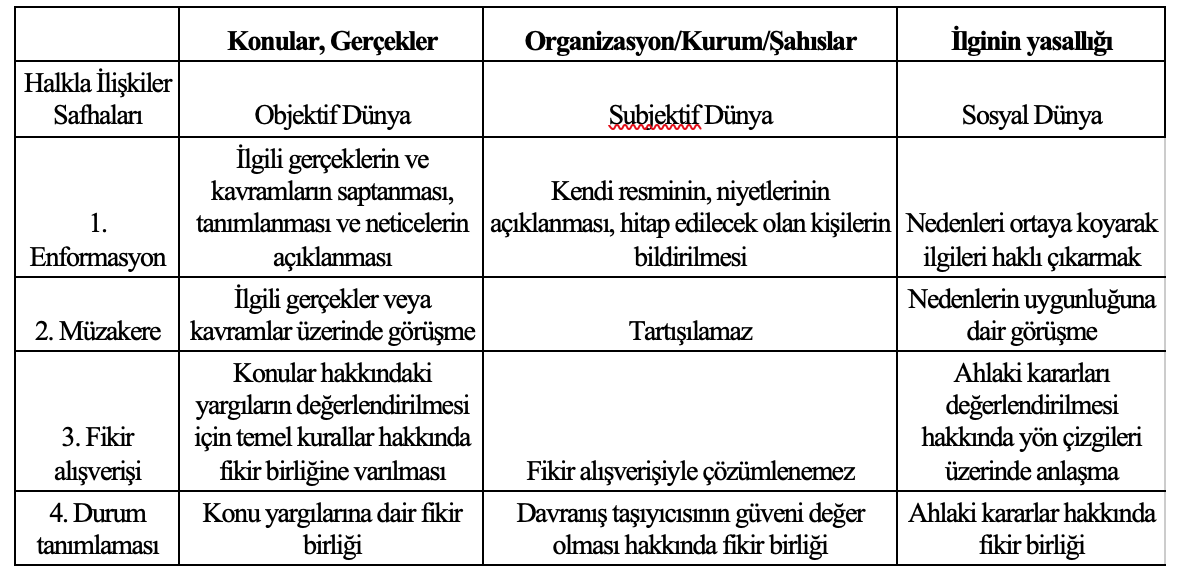
\includegraphics[width=0.95\linewidth,height=0.95\textheight]{tablolar-sekiller/tablo-1.2} \caption{Kaynak: (Ayla Okay ve Okay, 2002: 95)}\label{fig:unnamed-chunk-1}
\end{figure}

Habermas'ın iletişimsel eyleminin temeli; anlaşılabilirlik, gerçeklik, güvenilirlik ve haklılık/meşruluk kavramlarından oluşmaktadır. Anlaşılabilirlikte, mesajın anlaşılır olması; gerçeklikte mesajların gerçeklere dayanıyor olması ya da öyle kabul edilmesi; güvenilirlikte mesajı taşıyanın dürüst olması; haklılık/meşrulukta ise, mesajların karşılıklı olarak tanınan değerler temelinde kabul edilebilir olması gereklidir (akt. Kuş, 2019; Ralph Tench, 2017). Bu bağlamda, iletişimsel eylem sürecine dâhil olmak isteyen tarafların yukarıdaki dört maddeyi göz önünde bulundurması önemlidir.

\hypertarget{organizasyon-teorisi-yaklaux15fux131mlarux131}{%
\subsection{Organizasyon Teorisi Yaklaşımları}\label{organizasyon-teorisi-yaklaux15fux131mlarux131}}

Grunig ve Hunt'un halkla ilişkiler uygulamalarını dört modelle tanımladığı organizasyon teorisi yaklaşımı, organizasyon ile hedef kitleleri arasındaki iletişimi esas almaktadır. Günümüzde, halkla ilişkiler kâr ve sosyal amaçlı olarak kullanılmaktadır. Çevre ve iklim konuları ile ilgili farkındalığın oluşturulması, toplumsal algının dönüştürülmesi için bu dört modelin ayrı ayrı kullanılabileceği noktalar bulunmaktadır. Tezin araştırma bölümünde iklim aktörlerinin iletişimlerinde hangi halkla ilişkiler modellerini kullandıkları araştırılmıştır. Hem literatürde hem de araştırma bağlamında, bu dört model önem arz etmektedir.
Grunig ve Hunt (1984) grunig1984managing halkla ilişkiler faaliyetlerini dört farklı model olarak kategorize etmişlerdir:

\begin{enumerate}
\def\labelenumi{\arabic{enumi}.}
\tightlist
\item
  Basın Ajansı Modeli,
\item
  Kamuoyunu Bilgilendirme Modeli,
\item
  Çift Yönlü Asimetrik Model,
\item
  Çift Yönlü Simetrik Modeli.
\end{enumerate}

James Grunig'e göre, 1850'lerden itibaren halkla ilişkiler uygulamaları dört ayrı model altında incelenebilir. Grunig; 1850-1900 yılları arası uygulamaları ``basın ajansı ve tanıtım'' modeli olarak isimlendirirken 1900'den 1920'ye kadar yılları arasındaki halkla ilişkiler faaliyetlerini ``kamuyu bilgilendirme'' başlığı altında irdelemiş, 1920'lerden itibaren halkla ilişkiler uygulamalarını ``iki yönlü asimetrik model'', 1960'ların sonu ve 1970'lerden sonraki uygulamalarını ``iki yönlü simetrik model'' olarak ele almıştır (s. 95). \citep{peltekoglu2016halkla}

\textbf{Tablo 1.3:} Grunig ve Hunt'a Göre Halkla İlişkiler Davranışının Dört Modeli.

\begin{figure}
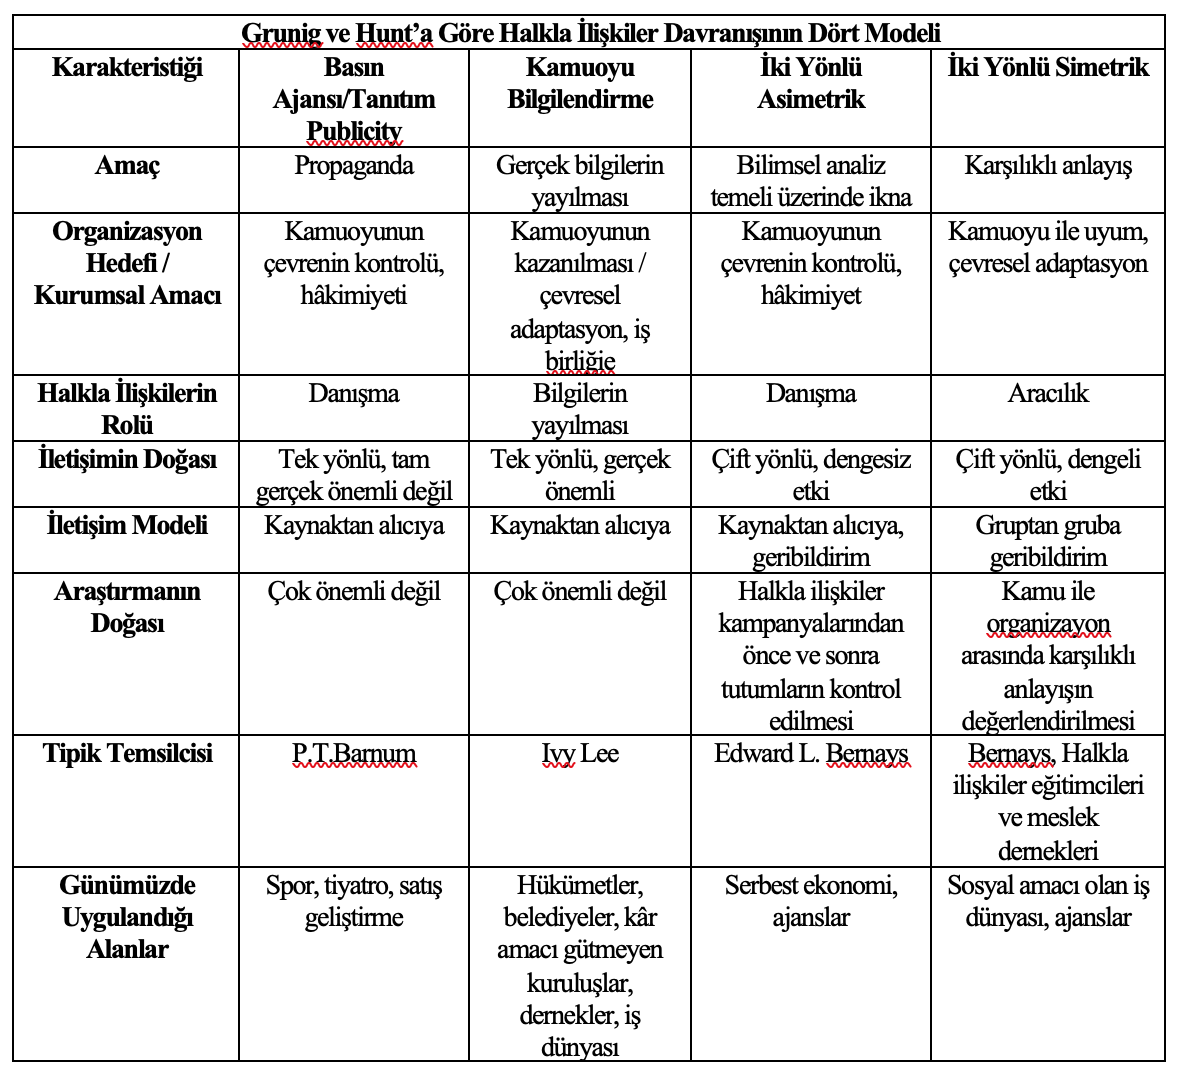
\includegraphics[width=0.95\linewidth,height=0.95\textheight]{tablolar-sekiller/tablo-1.3} \caption{Kaynak: (Mavimbela ve diğerleri, 2018: 42)}\label{fig:unnamed-chunk-2}
\end{figure}

Bu dört model, bir kuruluş ile paydaşları arasında oluşabilecek farklı iletişim biçimlerini tanımlamaktadır. Daha spesifik olarak bu dört model iletişim faaliyetleri bakımından iki şekilde farklılık göstermektedir: birincisi, iletişimcinin niyetine göre, yani kişileri ikna etmek, etkilemek veya kişilerle kurum arasında ortak bir anlayış yaratmak için yapılmaktadır. İkincisi; iletişimin yönüne göre yani, tek yönlü, iki yönlü asimetrik veya iki yönlü simetrik olup olmamasına göre yapılan faaliyetlerdir. Sosyal medya, genellikle paylaşılan anlayış yaratabilen iki yönlü simetrik iletişim ile ilişkilendirildiğinden modeller, halkla ilişkiler uygulayıcılarına sosyal medyayı kendi iletişim karışımlarına nasıl dâhil edebilecekleri konusunda faydalı bilgiler sağlamaktadır (s. 40). \citep{mavimbela2018perceived}

Modellerden ilki olan basın ajansı/tanıtım modeli; halkla ilişkileri bir mesajlaşma, tanıtım, bilgilendirme ve medya-ilişkileri işlevi olarak görmektedir. Bu yaklaşımı kullanarak, halkla ilişkiler uygulayıcıları, paydaşların davranışlarını etkilemek için ikna ve manipülasyon yöntemlerini kullanabilirler (Mavimbela ve diğerleri, 2018: 40). Uygulayıcılar genellikle eksik, çarpık veya yarı doğru bilgilerle ilgili kuruluşun inancını yayarlar (s. 21). \citep{grunig1984managing} Basın ajansı modelinin bahsedilen kötü yönleri dışında, bu model ikna düzeyi yüksek propaganda teknikleri ile bazı kitleleri; hızlı bir şekilde çevre ve iklim konularında farkındalık yaratıp onlarda duyarlılık oluşturması mümkündür.

Grunig ve Hunt'un halkla ilişkiler modellerinden ikincisi, kamuoyunu bilgilendirme modelidir. Bu modelde, bilgiyi ve tutumları değiştirme amacı olmaksızın izleyicilere dağıtılır. Halkla ilişkiler uygulayıcısı burada bir gazeteci gibi hareket etmektedir (s. 21-22). \citep{grunig1984managing} Model; halkla ilişkiler uygulayıcılarının sosyal medyayı, geleneksel medyayı, haber bültenlerini ve yayınları kullandıkları gibi ilk olarak bir bilgi dökümü olarak kullandığını belirtmektedir. Teori; ayrıca, web sitelerinin bilgiyi yaymak, yayınlarını ve haber bültenlerini yayımlamak için kullanıldığını öne sürer. Facebook ve YouTube gibi sosyal medya uygulamaları, kamuoyu bilgilendirme modeline uygundur (Mavimbela ve diğerleri, 2018). {[}mavimbela2018perceived{]}

İki yönlü asimetrik halkla ilişkiler, uygulayıcıların amaçları için en iyi bilimsel ikna yöntemi olarak tanımlanmıştır. Ancak, daha çok basın temsilcisi/yayıncısının işlevine benzer bir işleve sahiptir. Toplumu, kuruluşun bakış açısını kabul etmeye ve kuruluşları desteklemeyi amaçlayan hedef grupları davranışlarını oluşturmak için tutum ve davranışlarla ilgili sosyal bilim teorisi ve araştırmaları kullanılır. Basın temsilcisinin/yayıncısının ikna etme girişimleri ise, bilimsel olmaktan çok daha sezgiseldir (s. 22). \citep{grunig1984managing}

Son olarak, iki yönlü simetrik modelde uygulayıcılar, kuruluşlar ve onların kamuları arasında arabulucu olarak hizmet etmektedir. Bu hedefler, kuruluşlar ve halkları arasında karşılıklı anlayışı sağlamaktadır. Bu uygulayıcılar da sosyal bilim teorilerini ve yöntemlerini kullanabilirler; ancak halkla ilişkilerin planlanması ve değerlendirilmesi için genellikle ikna teorilerinden ziyade iletişim teorilerini kullanırlar (s. 22). \citep{grunig1984managing}

Çalışmanın ileri bölümlerinde, çevre ve iklim iletişiminde kamuoyunda bir tutum ve davranış değişikliği oluşturmak için farklı iletişim yaklaşımları ele alınacaktır. Bu bölümde anlatılan halkla ilişkiler modelleri, ileri bölümlerde anlatılacak iletişim yaklaşımlarıyla birlikte yorumlanması ve oluşturulmak istenen davranış ve tutum değişiminin istenilen biçimde sağlanması açısından önem arz etmektedir.
Hem simetrik modelle bağlantısı hem de araştırmanın bulguları diyalojik iletişim yaklaşımı bağlamında ele alınacağından dolayı bir sonraki başlıkta diyalojik iletişim olgusu anlatılacaktır.

\hypertarget{diyalojik-iletiux15fim-olgusu-ve-halkla-iliux15fkiler}{%
\section{Diyalojik İletişim Olgusu ve Halkla İlişkiler}\label{diyalojik-iletiux15fim-olgusu-ve-halkla-iliux15fkiler}}

Diyalojik iletişim olgusu, halkla ilişkilerin simetrik modeli ile ilişkilendirilmektedir. Diyalojik halkla ilişkiler kavramı, Kent ve Taylor'un `Building Dialogic Relationship Through the The Wold Wide Web' çalışmasıyla literatüre girmiştir. İki yönlü halkla ilişkiler modelini uygulayan kurum / kuruluşlar; problemleri sonuçlandırmak, karşılıklı anlayışı geliştirmek ve hedef gruplarıyla bağ kurmak için diyalog kurmaktadırlar. Sosyal medyanın yorumlanması ve değerlendirilmesi bakımından diyalojik iletişim önemli bir kuramsal çerçeve sunmaktadır (s. 34). \citep{gunay2018sosyal} Diyalojik iletişim ve sosyal ağlardaki iletişim üzerinden birçok araştırma yapılmaktadır. Bunlardan bazıları literatür ve araştırma bağlamında ele alınmaktadır.

Halkla ilişkiler çalışmaları, genellikle Grunig ve Hunt'un dört halka ilişkiler modelleri olan basın ajansı, kamuyu bilgilendirme, iki yönlü asimetrik ve iki yönlü simetrik iletişim modellerini ele almaktadır. Uygulayıcılar tarafından bu dört modelden en çok kullanılması istenen iki yönlü simetrik modeldir. Kent ve Taylor, iki yönlü simetrik iletişim ve diyalojik iletişim arasındaki bağlantıyı süreç ve ürün ilişkisi olarak görmektedir. İki yönlü simetrik iletişimin teorik zorunluluğu, bir organizasyonun ve hedef gruplarının etkileşimli olarak iletişim kurabileceği bir prosedür sağladığını ifade etmektedir. İki yönlü halkla ilişkiler için yapılandırılmış sistemler, süreçler ve kurallar oluşturulmalıdır. Diyalojik iletişimde ise bir ilişkinin varlığı karşılıklı ilişkisel bir etkileşime atıfta bulunur. Diyaloğun bir süreçten başka bir ürün olduğu kabul edilir (s. 323). \citep{kent1998building}

Teknolojinin kendisi ilişkileri tek başına oluşturamaz, organizasyon ve kamu arasındaki ilişkide nasıl kullanıldığı önemlidir. Facebook, Twitter, Instagram gibi uygulamalar bir işi gerçekleştirme yeteneğine sahiptirler. Paydaşlarla sağlam, uzun süreli ilişkiler kurma deneyimli halkla ilişkiler uygulayıcılarına bağlıdır. Bu araçlar yalnızca diyalojik iletişim fırsatının var olduğu alanlar yaratır. Diyalojik iletişim açısından doğru araçların kullanılması halkla ilişkiler uygulayıcısının sorumluluğundadır (s. 341). \citep{rybalko2010dialogic}

Kent ve Taylor, organizasyonların hedef gruplarıyla web üzerinde diyalojik iletişim kurmaları için bir çerçeve sunmaktadır. Bu iletişimi sağlamak için de beş unsur belirlemişlerdir: Diyalojik döngü, bilginin kullanışlılığı, web için yeniden ziyaretçi sağlama, web ara yüzünün kullanıcı dostu olması ve ziyaretçilerin elde tutulması. \citep{kent1998building}

\textbf{Diyalojik Döngü:} Organizasyonlar ile hedef grupları arasındaki iletişimi geliştirme adına bir dizi fırsatlar sunmaktadır. Bu döngü, hedef grupların organizasyonları sorgulamasına imkân verir ve aynı zamanda kurumlara da hedef gruplardan gelebilecek sorunların, endişelerin, problemlerin yanıtlanması gibi fırsatlar sunmaktadır.

\textbf{Bilginin Kullanışlılığı:} Organizasyonların web sitelerinin hedef gruplarına yönelik önemli bilgiler sağlamak üzere özel bilgilere yer vermesi anlamına gelir. Bir web sayfası, halkla ilişkiler aracı olarak; sadece organize bilgiler dışında, tüm hedef gruplarına açık bir şekilde onların olumlu bir tutum oluşturması gerektiği vurgulanır. Bilginin kamuya açık hale getirilmesi, hedef gruplarıyla iletişimin geliştirilmesinin ilk adımı olarak görülür. Kişiler arası iletişimde olduğu gibi bireylerin birbirleri hakkında bilgi edinmesi, o ilişkiyi geliştirebiliyorsa bu durum kurum ve hedef grupları için de geçerlidir. Sağlıklı gerçek bir ilişki kurulacaksa hedef gruplarının problemleri ve endişeleri kurumlar tarafından dikkate alınıp değerlendirilmelidir. Bilgi açık hale getirilirken hedef gruplarının problemleri ve endişeleri karşısında, onlarla tartışmaya girmeden iletişim kurulması ve paydaş olarak diyaloğa girilmesi önerilir.

\textbf{Yeniden Ziyaretçi Sağlama:} Web sayfalarının güncel bilgiler, değişen konular, özel forumlar, yeni yorumlar, çevrimiçi soru-cevap gibi özellikler içermesi, kullanıcıların tekrar ziyaret etmelerine yöneliktir. Bilginin güncellenmesi ve ilgi çekici içeriklerin yer alması, halkla ilişkilerin tek yönlülüğünü temsil eder. Bu tür içerikler, halkla ilişkiler uygulayıcılarının bir stratejisi olsa da diyalojik stratejiler daha çok tercih edilmelidir. Sık sorulan sorular, bilgi sağlayıcı linkler ve indirilebilir bilgi dokümanları, tekrar ziyareti sağlayan özellikler olarak belirtilir (s. 329). \citep{kent1998building}

\textbf{Arayüzün Kullanıcı Dostu Olması:} Dördüncü unsur olarak web sitelerinin kullanıcı dostu olması, kolay bir kullanılabilirliğe sahip olması gerektiğidir. Siteye bilgi almak için gelen ya da internette gezinirken siteye uğrayan kişiler için sitenin kolay kullanılabilir ve anlaşılabilir olması, sitede ziyaretçilerin uzun dakikalar kalmasını sağlar. Web sitesinden zengin ve eşsiz içerikler yer almalıdır (s. 329). \citep{kent1998building} Ziyaretçilerin sitede uzun kalma süreleri ve ilgili web sitesinin diğer sayfaları üzerinde gezinmeleri, arama motorları için sitenin ilgili konuda bir ağırlığının olduğunu gösterir. Bu nedenle, web sitesi arama sonuçlarında daha fazla görünür hale gelecektir. Bu ilke, Twitter'in standart bir ara yüze sahip olması nedeniyle değerlendirilmeye alınmamıştır.

\textbf{Ziyaretçilerin Elde Tutulması:} Bu beşinci unsur, web sitesine gelen kullanıcıların yanlış yönlendirilmemesini kapsar. Web tasarımcılarının, ziyaretçileri yanlış yönlendiren linkler noktasında dikkatli olmaları gerektiği vurgulanır. Web sitesinde çok fazla reklam ve sponsorlu bağlantıların yer alması, ziyaretçilerin siteden hızlı bir şekilde ayrılmalarına neden olur. Diyalojik iletişim için kurum sitelerinin ziyaretçilerle reklam ve pazarlama amaçları yerine, karşılıklı etkileşim alabilecekleri iletişim faaliyetlerine yönelmeleri tavsiye edilir (s. 330). \citep{kent1998building} Clickbait ve pop-up benzeri uygulamalardan kaçınılması gerektiği vurgulanır.

Kent ve Taylor'un diyalojik iletişim için ortaya koymuş olduğu beş unsur, web sitelerinin teknik ve yapısal unsurlarını ortaya koymaktadır. Kurumlar, diyalojik iletişim kurmak için web sitelerinde bu unsurlara dikkat etmelidir. Sosyal medya üzerindeki halkla ilişkiler uygulamalarında da diyalojik iletişim kullanılır. Reklam ve pazarlamaya yönelik tek yönlü iletişim faaliyetlerinin dışında, sosyal medya sayesinde organizasyonlar ve hedef gruplar arasında karşılıklı bir diyalog ve etkileşim ortamı oluşmuştur. Web sitelerinin kolay kullanılabilirliği, mobil uyumluluğu, hızlı çalışması, blog ve sosyal ağ uygulamalarında vakit geçirilebilecek içeriklerin üretilmesi gibi unsurlar bu süreçleri kapsamaktadır. Kullanıcı dostu içerikler paylaşılırken sonrasında ziyaretçilerle iletişimin devam etmesi için soru, görüş ve yorumlar gibi karşı taraftan gelebilecek geri dönüşlere de açık olunması; diyalog oluşması ve halkla ilişkiler faaliyetleri açısından da önem arz etmektedir.
Son zamanlarda Twitter gibi sosyal ağ uygulamalarında diyalojik iletişim üzerine araştırmalar yapılmıştır. Örneğin, \citet{thelen2021dialogic} 112 PR ajansının Twitter paylaşımlarını diyalojik iletişim bağlamında tartışmıştır. \citet{wang2020dialogic} ise, diyalojik iletişim fenomeni içinde hem kâr amacı taşıyan hem de kâr amacı taşımayan kuruluşlardan gelen tweetleri karşılaştırmıştır. Ayrıca, diyalojik iletişim unsurlarının kullanımı ve kullanım boyutları araştırılmıştır. Her iki makale de araştırma tasarımında kullanılmıştır. Başka bir araştırmada da Fortune 500 şirketlerinin Twitter profillerinin içerik analizi de yapılmıştır. \citep{rybalko2010dialogic}

Halkla ilişkiler; imaj, algılar, mesajlaşma, itibar, markalar, bütünleşmiş pazarlama iletişimi, yatırım getirisi (ROI), stratejik iletişim, kurumsal sosyal sorumluluk projeleri gibi kavramlara odaklanmaktadır. Halkla ilişkiler uygulayıcıları, yeni dijital medyayı, düşünme biçimlerini değiştiren ve halkla ilişkiler uygulamalarını şekillendiren devrimci bir güç olarak görmektedir (s. 1). \citep{grunig2009paradigms} Bu noktada, organizasyonlar da halkla ilişkiler uygulamalarını, pazarlama faaliyetlerini ve diğer iletişimlerini sosyal ağlar üzerinden sağlamaktadır. Bu bağlamda, Twitter önemli bir sosyal ağ uygulaması olarak karşımıza çıkmaktadır.

Halkla ilişkiler uygulayıcıları, ilk olarak çevrimiçi medyayı, geleneksel medyayı kullandıkları şekilde, bir bilgi dökümü olarak kullanmışlardır. Web siteleri; bilgiyi yaymak, yayınları ve haber bültenlerini yayımlamak için kullanılmıştır. Çalışan intranetleri, büyük ölçüde çevrimiçi haber bültenleri olmuştur. E-postalar ise, büyük ölçüde promosyon mesajlarını iletmek için kullanılmıştır. Sosyal medya da viral pazarlama gibi tekniklerle pazarlama mesajlarını yaymak için kullanılmaktadır (s. 7). \citep{grunig2009paradigms}

Dijital medyanın; halkla ilişkilerin stratejik yönetim paradigması için mükemmel bir şekilde uygun olan diyalojik, etkileşimli, ilişkisel ve küresel özellikleri bulunmaktadır (s. 6). \citep{grunig2009paradigms} Twitter gibi mecralar hem organizasyonlar hem de hedef grupları arasında Grunig'in gösterdiği bu özellikleri taşımaktadır. Sosyal ağlar üzerindeki hareketlilik, veri miktarı, farklı veri yapıları, teknolojinin dinamik gelişimi araştırmacılar için muazzam bir çalışma alanı sunmaktadır.

Phillips'in LeverWealth blogunda dijital araçların; basın ajansı/tanıtım, bilgilendirme, iki yönlü asimetrik ve iki yönlü simetrik dört halkla ilişkiler modeline nasıl uyduklarını göstermek için bir model oluşturdu. \citep{phillipsleverwealth} Phillips'e göre, sosyal medya; halkla ilişkiler faaliyetlerine uygun diyalojik, etkileşimli ve ilişkisel özelliklere sahiptir. Bu yaklaşımın halkla ilişkiler uygulayıcılarını; geleneksel tek yönlü iletişim, mesaj odaklı ve asimetrik iletişimden vazgeçmeye zorlaması beklenebilir (s. 40). \citep{mavimbela2018perceived}

Sosyal medya, insanların içerik, fikir, deneyim ve görüşlerini paylaşmasına imkân sağlayan önemli özelliklere sahiptir. Diğer katılımcılar, geri bildirim ve paylaşım yaparak katılımcıların içeriğe katkı sunabilmesi etkileşimli iki yönlü iletişimi kolaylaştırmaktadır. İki yönlü iletişim platformları, halkla ilişkiler uygulayıcılarının paydaşlarıyla etkileşim kurmalarına ve çevrimiçi paydaşlara ulaşabilecek etkili kampanyalar tasarlamalarına olanak tanımaktadır (s. 39-40). \citep{mavimbela2018perceived} İki yönlü asimetrik model uygulayıcıları, hedef gruplarını organizasyonun istediği gibi davranmaya ikna etme ve manipülasyon için kullanır. Bu modelde örgütsel iletişimin amacı, daha çok kuruluşun kendi mesajını daha ikna edici hale getirmektir. Phillips'e göre kuruluşlar, çoğunlukla paydaşların algılarını, tutumlarını veya davranışlarını değiştirmek için asimetrik iki yönlü iletişim modelini kullanır (s. 40-41). \citep{mavimbela2018perceived}

Dijital medya; küresel, stratejik, iki yönlü, etkileşimli, simetrik/diyalojik ve sosyal olarak sorumlu hale getirme gibi potansiyellere sahiptir. Halkla ilişkilerin dijital medyayı tam olarak kullanabilmesi için uygulayıcılar ve akademisyenler; halkla ilişkileri sembolik, yorumlayıcı bir paradigma yerine, davranışsal, stratejik bir yönetim paradigması olarak yeniden kurumsallaştırmalıdır (s. 1). \citep{grunig2009paradigms} Grunig'e göre organizasyonlar; kendi hedef kitlesi olmayan gruplarla sosyal ağlar üzerinde iletişim kurabilir ve onlarla etkileşim kursa dahi bu durum organizasyonların hedef kitlesi olmayan gruplarla ilişki geliştirmesini gerektirmediğini belirtmektedir. Organizasyonların herkesle iletişim kuracak ne zamanları ne de kaynakları olduğunu ifade etmektedir. Her ne kadar organizasyonlar, hedef kitlesi içerisinde yer almayan kişilerle iletişim kursa da halkla ilişkilerin organizasyonun mevcut hedef kitle ilişkileriyle ilgili olduğunu vurgulamaktadır (s. 6). \citep{grunig2009paradigms} Her ne kadar bu durum çok genel bir ifade olsa da özellikle iklim, çevre ve savaş gibi tüm dünyayı etkileyecek konularda devletler, bağımsız kuruluşlar ve sivil toplum kuruluşları; her bir toplumu ve bireyi dikkate almak durumunda kalabilirler. Özellikle uluslararası sivil toplum kuruluşları, faaliyetlerini herkese ulaştırma noktasında iletişimlerini gerçekleştirirler.

\textbf{Şekil 1.3:} Phillips'in Dijital İletişim Araçları Modeli.

\begin{figure}
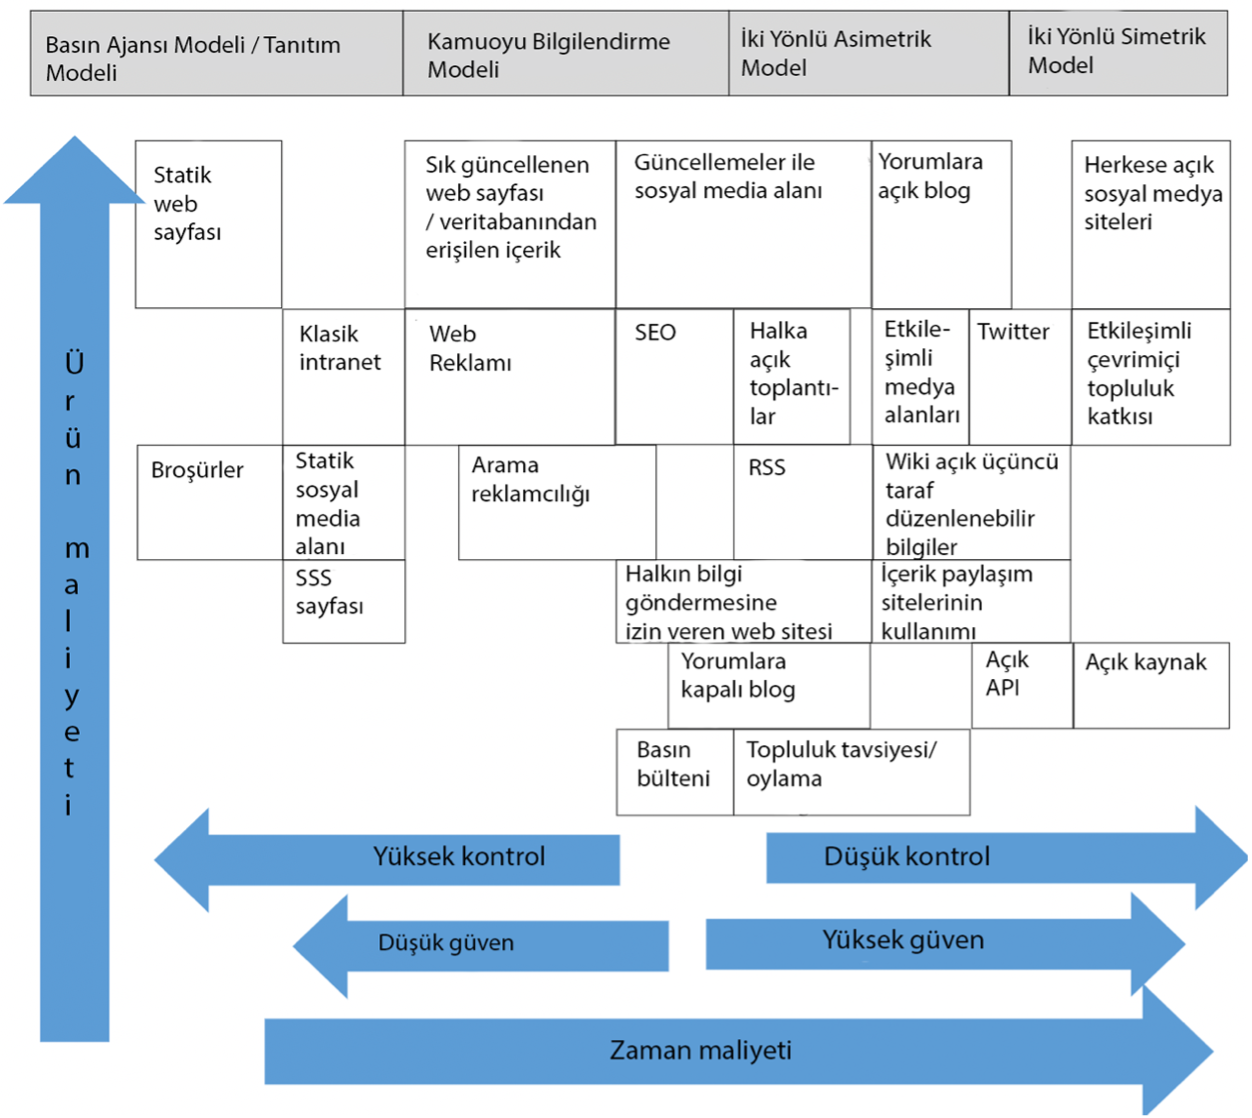
\includegraphics[width=0.95\linewidth,height=0.95\textheight]{tablolar-sekiller/sekil-1} \caption{Kaynak: (Mavimbela ve diğerleri, 2018: 42)}\label{fig:unnamed-chunk-3}
\end{figure}

Kaynak: (Mavimbela ve diğerleri, 2018: 42)

Yukarıda (Şekil 1.3), Phillips'in dijital iletişim araçlarının Grunig ve Hunt'un dört modeline göre uyarlanması gösterilmektedir. Modelde dört değişken bulunmaktadır. İlk değişken zaman maliyetidir. Şekilde 1.3'te, halkla ilişkiler faaliyetlerinin sol üst tarafta basın ajansı ve kamuoyu bilgilendirme modelleri, sağ üst tarafta ise asimetrik ve simetrik modeller görünmektedir. Sağ taraftaki asimetrik ve simetrik modellerin daha çok zaman maliyeti olması beklenmektedir. Buradan sosyal medyayı, PR faaliyetleri için kullanmak isteyenlerin daha çok zaman harcaması ve bunun yönetilmesi gerektiği ifade edilebilir. Öte yandan, dış paydaşlar açısından sosyal medya iletişiminin anlık doğası, bir fayda olarak görülebilir.

İkinci değişken kontrol düzeyidir. Şekil 1.3'ün sağ tarafındaki halkla ilişkiler faaliyetlerinin (sağ tarafta yer alan asimetrik ve simetrik modellerin) iletişim içeriği ve işlemleri üzerine sol tarafta yer alan faaliyetlere göre (basın ajansı veya kamuoyu bilgilendirme modeli) daha az kontrole sahip olma beklenmektedir. Bundan dolayı, sosyal medyayı halkla ilişkiler faaliyetlerine dâhil eden uygulayıcılar için bir zorluk ve kontrol eksikliği yaratabilir. Bu, bireysel çalışanların kötüye kullanması gibi başka sorunlara yol açabilir. Bu durumun karşılığında dış paydaşlar için iletişimin getirdiği şeffaflık kurumsal itibar için bir fayda sağlayabilir.

Modelde gösterilen üçüncü değişken güven düzeyidir. Şekil 1.3'e göre, sağ tarafta temsil edilen halkla ilişkiler faaliyetlerinin (iki yönlü simetrik model), sol taraftakilerden (basın ajansı veya kamuoyu bilgilendirme) daha fazla güven sağlaması beklenmektedir. Örnek olarak; sosyal medya aracılığıyla paydaşlara kurumsal bilgiler sağlanması bir mahremiyet kaybı getirebilirken halkla ilişkiler uygulayıcılarının kuruluşun imajına zarar verebilecek yanlış bilgiler vermelerinin de güven kaybına sebep olabileceği de ifade edilmektedir. Bu kurumların yönetmesi gereken bir zorluktur. Ancak, dış paydaşların bakış açısından; iki yönlü simetrik modelde faydalı ve dürüst iletişim, paydaş ilişkilerini oluşturmak ve yönetmek, kurumsal imajı geliştirmek gibi faydalar sağlayabilir.

Dördüncü değişken üretim maliyetidir (sol tarafta). Şekil 1.3'te yer alan iletişim araçlarından bazıları, özellikle iki yönlü iletişim sağlayanlar, maliyetlidir. Bu nedenle, yüksek maliyet, kurumlar açısından bir zorluk olarak görülebilir. Bununla birlikte, bu araçların kullanımı, faydalı sonuçlar ortaya çıkarırsa, sosyal araçların kullanılmasının uygun maliyetli görülmesi de mümkündür.

Çalışmanın dördüncü bölümünde, Phillips'in ``Dijital İletişim Araçları Modeli'' çerçevesinde Twitter verileri değerlendirilmiştir. Twitter'da kurumların mesajları, bu modelin belirtilen değişkenleriyle ele alınarak dört-model bağlamında bir yaklaşım geliştirilmeye çalışılmıştır.

\hypertarget{halkla-iliux15fkiler-ve-dijital-medya}{%
\section{Halkla İlişkiler ve Dijital Medya}\label{halkla-iliux15fkiler-ve-dijital-medya}}

Sosyal medya, halkla ilişkiler alanı için önemli etkilere sahiptir. Araştırmacılar, kuruluşların sosyal medya kullanımıyla elde edebilecekleri birçok faydayı tespit etmişlerdir. Dijital medyanın yaygın kullanımı, halkla ilişkiler (PR) uygulayıcılarının bilgiyi paylaşma ve iletme şeklini değiştirmede önemli bir rol oynamaktadır \citep{komodromos2014study} ve onlara kendi kitleleriyle iki yönlü iletişim kurma fırsatı vermektedir (Saxton ve Waters, 2014). \citep{saxton2014stakeholders}

Diyaloğa girmek, halkla ilişkiler uygulamaları yapmak ve onları sürdürmek için etkili bir strateji olarak kabul edildiğinden (Bruning, Dials ve Shirka, 2008) \citep{bruning2008using}, internetin diyalojik iletişimi geliştirme potansiyelinin organizasyon-halk ilişkilerini olumlu yönde nasıl etkileyebileceğini araştıran birkaç çalışma bulunmaktadır. \citep{kelleher2009conversational, kent1998building} Sonuç olarak hem akademisyenler hem de halkla ilişkiler uygulayıcıları, hedef kitleleriyle iletişim kurmak ve etkileşime geçmek için en iyi yolları aramaktadırlar (Sundstrom ve Levenshus, 2017; Thelen ve diğerleri, 2021). \citep{sundstrom2017art}

\citet{rybalko2010dialogic} 'in yapmış oldukları araştırmaya göre, kuruluşların mevcut diyalojik iletişim stratejilerini tam olarak kullanmadıklarını tespit etmişlerdir. \citep{burnap2015} Dijital medya, halkla ilişkiler uygulayıcılarına hem platform olarak hem de yeni teknolojik araçlarla birçok alan açmıştır. Bu platformların ve araçların kullanımı için uygulayıcıların bu konularda kendilerini eğitmesi de gerekmektedir. Teknolojik gelişmeler, halkla ilişkiler faaliyetlerini de yeni boyutlara taşımaktadır.

Sosyal medya uygulamalarının yönetimi, halkla ilişkiler uygulayıcıları için önemli ve zaman alıcı bir işlev haline gelmiştir. Bu nedenle, sosyal medya uzmanı olarak ayrı bir iş dalı ortaya çıkmıştır. \citet{wright2017tracking} tarafından yürütülen bir uygulayıcı anketi, halkla ilişkiler uzmanlarının \%64'ünün çalışma zamanlarının \%11 ile \%50'sini bloglar ve diğer sosyal medya ile herhangi bir yerde geçirdiğini ortaya çıkarmıştır. Avrupalı uygulayıcılarla yapılan bir araştırma, sosyal medyayı \%55'inin günlük olarak ve \%27,2'sinin haftada birkaç kez işte kullandığını buldu. \citep{moreno2015does} İletişim uzmanları, kuruluşların sosyal medya araçlarını, ilişki kurma \citep{cho2014} ve pazarlama iletişimi \citep{estanyol2012marketing} dâhil olmak üzere çok sayıda nedenle kullandığını bulmuşlardır. Dijital medyanın gelişmesiyle birlikte, iş dünyası ve hedef grupları arasında yeni davranışlar ortaya çıkmıştır. Sosyal medya paydaşların kuruluşlarla bağlantı kurma şeklini ve profesyonel iletişimcilerin kendi ürün ve iletişim biçimlerini, onların paydaşlarla arasında fikirler üretme şeklini de değiştirmektedir. \citep{thelen2021dialogic, young2013thought}

\hypertarget{sosyal-medya-etkileux15fimi}{%
\section{Sosyal Medya Etkileşimi}\label{sosyal-medya-etkileux15fimi}}

Sosyal medya katılımı ve kanaat önderliği; ilişkilerin kurulmasına, geliştirilmesine ve kuruluşların kamularıyla olan güvenini ve itibarını artırmaya yardımcı olabilir. İklim aktörleri bağlamında, iklim kriziyle ilgili halkla ilişkiler uygulamalarının sosyal medyada etkin bir şekilde nasıl yürütüleceğinin bilinmesi büyük önem taşımaktadır.

Teknolojik ilerlemelerin bir sonucu olarak, bilim insanları ve uygulayıcılar, kuruluşların sosyal ağlar gibi etkili platformlar aracılığıyla hedef gruplarla nasıl daha etkili bir şekilde iletişim kurabileceklerini anlamaya çalışmaktadırlar. Son yıllarda, halkla ilişkiler uzmanları internetin halkla ilişkiler uygulaması üzerindeki rolünü ve etkisini araştırmaktadırlar. Twitter gibi sosyal medya platformları, tüketicilere kuruluşlarla etkileşimlerinde bir ses ve artan güç sunmaktadır.

Organizasyonlar ve hedef grupları arasındaki etkileşim, sosyal medyada önemli bir bileşendir. \citep{rybalko2010dialogic} Fikirler ve karşılıklı çıkar konuları üzerine anlamlı konuşmaların paylaşılması, stratejik katılım için zemin hazırlayacaktır. Düşünce liderliği; yenilik, bilgi ve farklı fikirlere dayanır \citep{mccrimmon2005thought} ve önemli paydaşları sosyal medyaya dâhil etmek için etkili bir araç olarak kullanılabilir. Sosyal medya aracılığıyla düşünce liderliğini gerçekleştirmeyi hedefleyen kuruluşlar, hangi fikirlerin önemli olduğunu tespit etmeli ve bu fikirleri stratejik olarak önemli kitlelere nasıl ileteceklerini bulmalıdır (Heath ve diğerleri, 2013; Teece, 2007).

Katılım kavramı, halkla ilişkilerde diyalog tartışmasının merkezinde yer almaktadır. Organizasyonların, etik olmak için hedef gruplarıyla diyalog kurulması gerektiği ifade edilmektedir. Bağlılık kavramı, yakınlık ilkesinin bir özelliği olarak ortaya çıkmaktadır. \citep{kent2002toward} Diyalojik yakınlık, ``kamuların kendilerini etkileyen konularda danışılması ve halklar için bu, onların taleplerini örgütlere ifade etmeye istekli ve yetenekli oldukları anlamına gelir''. Katılım, etkileşimde bulunanların karşılaşmalara tüm benliklerini vermeye istekli olduklarının kabulüdür. Katılım; erişilebilirliği, hazır bulunmayı ve etkileşime girme isteğini barındırmaktadır. \citep{taylor2014dialogic}

Tüm kuruluşlar; izleyicilerin ihtiyaç ve beklentilerini karşılayan içerik geliştirme, bunlardan yararlanma ve dağıtma potansiyeline sahiptir. Etkili bir şekilde yapılırsa bu tür bir iletişim, katılımı teşvik edebilir ve ilişkisel sonuçları iyileştirebilir. \citep{mersey2010engagement} Organizasyonlar, içeriği etkin bir şekilde yaymak ve hedef kitleleriyle etkileşim kurmak için çevrimiçi medya kanallarına uyum sağlamalıdır.

Sosyal medya katılımıyla ilgili yapılan çalışmalara örnek olarak, Facebook gönderilerinde CEO'ların hedef gruplarının katılımı araştırılmıştır. İçerik analizi yöntemiyle, diyalojik iletişimin sosyal boyutunu da dâhil ederek, onun kavramsal çerçevesi genişletilmiştir. Araştırma sonucunda, CEO'ların diyalojik iletişim ilkelerini kullanmalarına rağmen, yine de tek yönlü iletişim stratejilerinin daha yaygın olduğu tespit edilmiştir. \citep{men2018social} Diğer bir araştırmada da Twitter içerikleri, diyalojik iletişim bağlamında değerlendirilip Twitter kullanıcılarının içeriklerle beğeni ve retweet kapsamında ne ölçüde etkileşime girdiği araştırılmıştır. \citep{wang2020dialogic}

Hedef gruplarının ilgisini çekecek bilgiler sağlanması, gerekli görülen durumlarda iki yönlü bir iletişim kurulması ve organizasyonların sosyal bir varlık olarak etkili ve uyumlu iletişim stratejileri oluşturması, kullanıcıların beğeni, yorum ve paylaşım yapmalarını etkili bir şekilde teşvik edecektir.

You can label chapter and section titles using \texttt{\{\#label\}} after them, e.g., we can reference Chapter \ref{intro}. If you do not manually label them, there will be automatic labels anyway, e.g., Chapter \ref{methods}.

Figures and tables with captions will be placed in \texttt{figure} and \texttt{table} environments, respectively.

\begin{Shaded}
\begin{Highlighting}[]
\FunctionTok{par}\NormalTok{(}\AttributeTok{mar =} \FunctionTok{c}\NormalTok{(}\DecValTok{4}\NormalTok{, }\DecValTok{4}\NormalTok{, .}\DecValTok{1}\NormalTok{, .}\DecValTok{1}\NormalTok{))}
\FunctionTok{plot}\NormalTok{(pressure, }\AttributeTok{type =} \StringTok{\textquotesingle{}b\textquotesingle{}}\NormalTok{, }\AttributeTok{pch =} \DecValTok{19}\NormalTok{)}
\end{Highlighting}
\end{Shaded}

\begin{figure}

{\centering 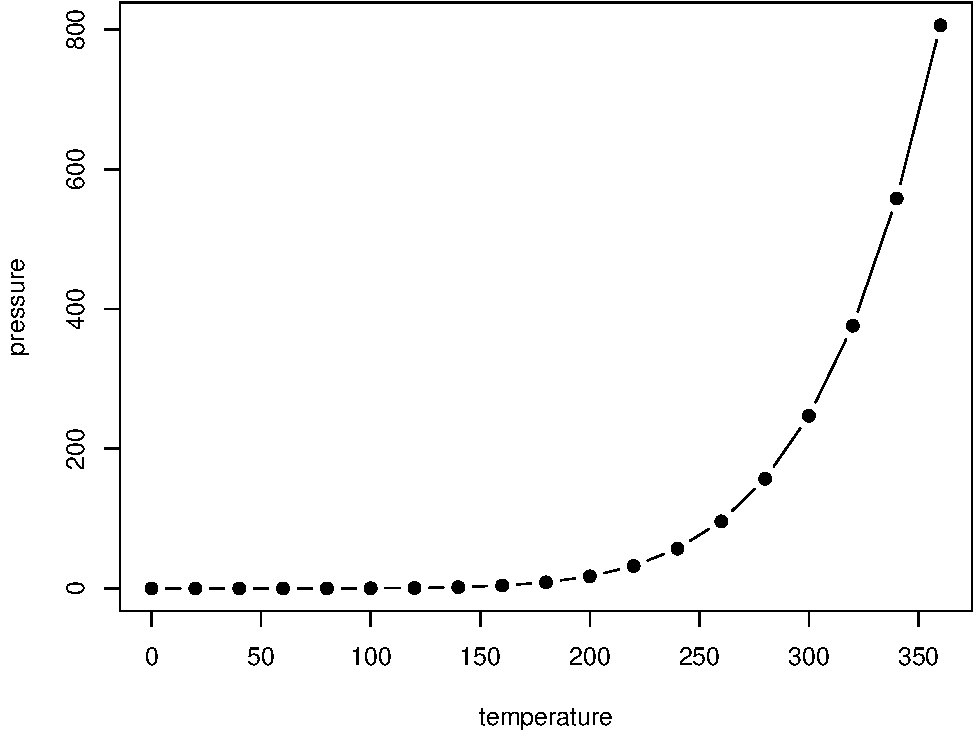
\includegraphics[width=0.8\linewidth]{01-BOLUM_files/figure-latex/nice-fig-1} 

}

\caption{Here is a nice figure!}\label{fig:nice-fig}
\end{figure}

Reference a figure by its code chunk label with the \texttt{fig:} prefix, e.g., see Figure \ref{fig:nice-fig}. Similarly, you can reference tables generated from \texttt{knitr::kable()}, e.g., see Table \ref{tab:nice-tab}.

\begin{Shaded}
\begin{Highlighting}[]
\NormalTok{knitr}\SpecialCharTok{::}\FunctionTok{kable}\NormalTok{(}
  \FunctionTok{head}\NormalTok{(iris, }\DecValTok{20}\NormalTok{), }\AttributeTok{caption =} \StringTok{\textquotesingle{}Here is a nice table!\textquotesingle{}}\NormalTok{,}
  \AttributeTok{booktabs =} \ConstantTok{TRUE}
\NormalTok{)}
\end{Highlighting}
\end{Shaded}

\begin{table}

\caption{\label{tab:nice-tab}Here is a nice table!}
\centering
\begin{tabular}[t]{rrrrl}
\toprule
Sepal.Length & Sepal.Width & Petal.Length & Petal.Width & Species\\
\midrule
5.1 & 3.5 & 1.4 & 0.2 & setosa\\
4.9 & 3.0 & 1.4 & 0.2 & setosa\\
4.7 & 3.2 & 1.3 & 0.2 & setosa\\
4.6 & 3.1 & 1.5 & 0.2 & setosa\\
5.0 & 3.6 & 1.4 & 0.2 & setosa\\
\addlinespace
5.4 & 3.9 & 1.7 & 0.4 & setosa\\
4.6 & 3.4 & 1.4 & 0.3 & setosa\\
5.0 & 3.4 & 1.5 & 0.2 & setosa\\
4.4 & 2.9 & 1.4 & 0.2 & setosa\\
4.9 & 3.1 & 1.5 & 0.1 & setosa\\
\addlinespace
5.4 & 3.7 & 1.5 & 0.2 & setosa\\
4.8 & 3.4 & 1.6 & 0.2 & setosa\\
4.8 & 3.0 & 1.4 & 0.1 & setosa\\
4.3 & 3.0 & 1.1 & 0.1 & setosa\\
5.8 & 4.0 & 1.2 & 0.2 & setosa\\
\addlinespace
5.7 & 4.4 & 1.5 & 0.4 & setosa\\
5.4 & 3.9 & 1.3 & 0.4 & setosa\\
5.1 & 3.5 & 1.4 & 0.3 & setosa\\
5.7 & 3.8 & 1.7 & 0.3 & setosa\\
5.1 & 3.8 & 1.5 & 0.3 & setosa\\
\bottomrule
\end{tabular}
\end{table}

You can write citations, too. For example, we are using the \textbf{bookdown} package \citep{R-bookdown} in this sample book, which was built on top of R Markdown and \textbf{knitr} \citep{xie2015}.

\hypertarget{iklim-deux11fiux15fikliux11fi-uxfczerine-kuramsal-bir-uxe7eruxe7eve}{%
\chapter{İKLİM DEĞİŞİKLİĞİ ÜZERİNE KURAMSAL BİR ÇERÇEVE}\label{iklim-deux11fiux15fikliux11fi-uxfczerine-kuramsal-bir-uxe7eruxe7eve}}

Çalışmanın ikinci bölümü, iklim değişikliği üzerine kavramsal bir çerçeve çizmeyi amaçlamaktadır. Bu bağlamda iklim değişikliği, iklim krizi ve küresel ısınma gibi kavramlar tanımlanmış ve aralarındaki nüanslar ele alınmıştır. İklim krizinin etkileri ve sonuçları tartışılmış, ayrıca iklim değişikliğine yönelik alınabilecek önlemler hakkında bilgi verilmiştir. Çevre ve iklim iletişimi bağlamında halkla ilişkiler uygulamalarını yorumlayabilmek için bu başlıklar önem arz etmektedir.

\hypertarget{iklim-deux11fiux15fikliux11fi-iklim-krizi-kuxfcresel-isux131nma-kavramlarux131-uxfczerine}{%
\section{İklim Değişikliği, İklim Krizi, Küresel Isınma Kavramları Üzerine}\label{iklim-deux11fiux15fikliux11fi-iklim-krizi-kuxfcresel-isux131nma-kavramlarux131-uxfczerine}}

İklim konusu çok kapsamlı bir konu olduğundan zaman içerisinde iklim değişikliği, küresel ısınma, iklim krizi gibi farklı tanımlamalarla ele alınmaktadır. İklim değişikliği günümüzde acil önlem alınması gereken bir problem olduğu için daha çok iklim krizi olarak karşımıza çıkmaktadır.

\hypertarget{iklim-deux11fiux15fikliux11fi}{%
\subsection{İklim Değişikliği}\label{iklim-deux11fiux15fikliux11fi}}

İklim değişikliği, sıcaklıklarda ve hava düzenlerinde uzun vadeli değişimleri ifade etmektedir. Bunlar, güneş döngüsünde meydana gelen değişiklikler gibi doğal olabilir, ancak 1800'lerden yana insan faaliyetleri; özellikle kömür, petrol ve gaz gibi fosil yakıtların yakılması iklim değişikliğinin ana nedeni olmuştur (United Nations). İklim, yer kürenin herhangi bir yerinde uzun yıllar boyunca yaşanan ya da gözlenen tüm hava koşullarının ortalama durumu olarak tanımlanmaktadır (s. 13). \citep{basucurehberi2008} Oxford Sözlüğü'nde, iklim değişikliği, sıcaklık, rüzgâr düzenleri ve yağıştaki değişiklikler de dâhil olmak üzere dünyanın hava koşullarındaki değişimler olarak tanımlanır. \citep{oxfordlearnersdict_climatechange} Özellikle, karbondioksit gibi gazların artması nedeniyle dünya atmosferinin sıcaklığındaki artış da bu kapsamda değerlendirilmektedir. Hükümetler arası İklim Değişikliği Paneli'ne (IPPC) göre; iklim değişikliği kavramı, iklim sisteminin sıcaklık ve yağış gibi temel özelliklerinde uzun bir zaman aralığında istatistiksel ölçümlerle tespit edilen doğal ve insan etkili değişimler olarak tanımlanmaktadır. \citep{dogan2011kuresel} Yine IPCC'nin başka bir tanımına göre; iklim değişikliği herhangi bir doğal değişiklik ya da insan faaliyetlerinin bir sonucu olarak ortaya çıkan değişiklik olarak açıklamaktadır (s. 515). \citep{pielke2004what} İklim değişikliği, araçsal ve temel bir araştırma biçimi olarak araştırmacılara disiplinler arası çalışma olanağı sunmaktadır (s. 3). \citep{serrao2018science} İklim değişikliği, sadece bilimsel bir problem değil, aynı zamanda sosyal bir problemdir ve bu nedenle toplumsal hareketlerin çözümüne ihtiyaç duymaktadır (s. 30). \citep{hansen2016communicating}

\hypertarget{kuxfcresel-isux131nma}{%
\subsection{Küresel Isınma}\label{kuxfcresel-isux131nma}}

İklim değişikliği ve küresel ısınma üzerine sosyal bilim literatürü, son yıllarda hızla büyümüştür ve artık tek bir çalışmada anlamlı bir incelemeye izin vermeyecek kadar genişlemiş ve çeşitliliği artmıştır (s. 197). \citep{mcadam2017social} Her ne kadar iklim değişikliği literatürü çok geniş de olsa bu bölümde iletişim çalışmalarını ilgilendiren iklim kavramları tanımlanmış; etkileri, sonuçları ve alınması gereken tedbirler açıklanmaya çalışılmıştır.

Önceki çalışmalar; küresel ısınma ve iklim değişikliği terimlerinin farklı siyasi çağrışımlara sahip olduğunu göstermektedir. Örneğin, partizan web siteleri üzerine yapılan bir araştırma, küresel ısınma kavramının daha politize olarak kullanıldığını, iklim değişikliğinin ise daha tarafsız bir kavram olarak kullanıldığını ortaya çıkarmıştır (s. 13). \citep{jang2015polarized} Shi ve arkadaşları, 2009-2018 yılları arasında atılan \#climatechange (iklim değişikliği) ve \#globalwarming (küresel ısınma) kavramlarının toplum tarafından nasıl algılandığını araştırmışlardır. İklim değişikliği ve küresel ısınma arasındaki fark ince gibi görünse de iki söylem arasında farklılıklar bulunmaktadır. Yapılan çalışmada, ``küresel ısınma'' Jang ve arkadaşlarının (2015) yapmış olduğu çalışmayı destekler nitelikte daha politize olduğu ve daha çok genel fenomenlere, özellikle sıcaklıkla ilgili anormalliklere odaklanırken iklim değişikliğinin ise daha bilimsel bir bakış açısına sahip olduğu ortaya çıkmıştır. Aşağıdaki Şekil 2.1'e bakıldığında kamusal söylemlerde ``iklim değişikliği'' kavramının ``küresel ısınma'' kavramına göre daha baskın olduğu görülmektedir. İnsanların bu kavramları ilişkilendirme biçimlerinde hala dikkate değer bir tutarsızlık olduğu sonucu ortaya çıkmıştır (s. 16). \citep{shi2020climatechange}

\textbf{Şekil 2.1:} İklim Değişikliği ve Küresel Isınma Tweet Karşılaştırması.

\begin{figure}
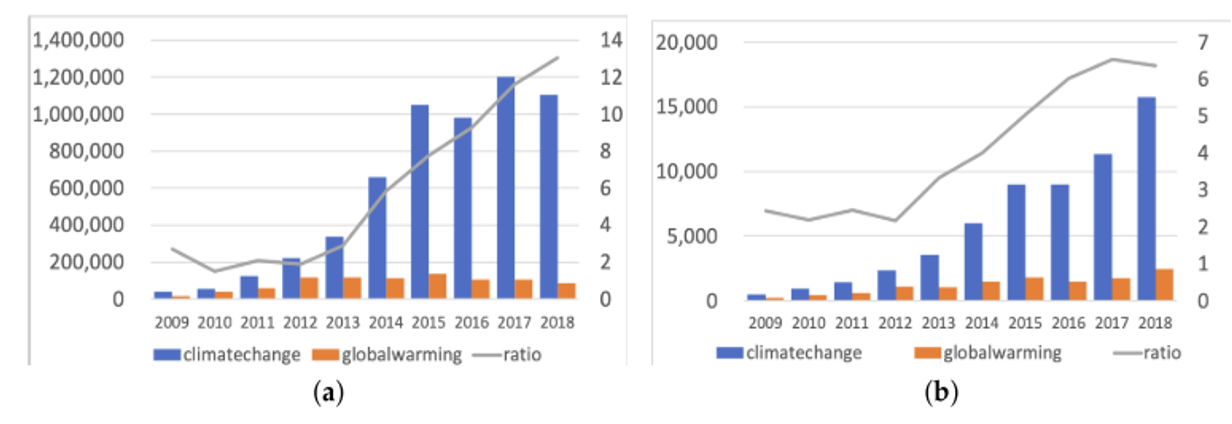
\includegraphics[width=0.95\linewidth,height=0.95\textheight]{tablolar-sekiller/seki-2-1} \caption{Kaynak: (Mavimbela ve diğerleri, 2018: 42)}\label{fig:unnamed-chunk-1}
\end{figure}

\begin{enumerate}
\def\labelenumi{(\alph{enumi})}
\tightlist
\item
  2009 ve 2018 yılları arasındaki \#climatechange (iklim değişikliği) ya da \#globalwarming (küresel ısınma) içeren tweetlerin sayısı (b) ``climate change'' ya da ``global warming'' içeren hastaglerin sayısı.
  Kaynak: (Shi vd., 2020: 16) \citep{shi2020climatechange}
\end{enumerate}

\hypertarget{iklim-krizi}{%
\subsection{İklim Krizi}\label{iklim-krizi}}

Günümüzde iklim değişikliği kavramı, bir iklim acil durumu haline gelmiştir. Dünya iklimi üzerindeki insan etkisinin uzun tarihi, küresel ve ulusal siyasi başarısızlıklar nedeniyle eyleme geçmekte yavaş kalınması, 2015 Paris Anlaşması'nın ardından iklim değişikliğinin hızı ve kapsamıyla 1,5°C'nin altında tutma ihtiyacının fark edilmesi, çok daha acil ulusal ve uluslararası politik eylemlerde bulunulmasını gerektirmektedir (s. 1). \citep{harvey2016climate}

Kriz kelimesi, klasik Yunan tıbbından gelmektedir. Krizi, hastalık metaforu üzerinden tanımlamak mümkündür: Bağışıklık sistemi hastalığı bastırdı ve hasta iyileşti ya da hastalık bağışıklık sistemini bastırarak hasta öldü. Kriz, işlerin aynı kalmayacağını ve değişimin olması gerektiğini vurgulamaktadır. Şu an insanlık da bu acil durum içerisindedir. Acil bir şekilde hastalığı tedavi etmeye yönelik eyleme geçilmesi gerekmektedir. Kriz anında ne olacağından çok ne yapılması gerektiğinin farkında olmak çok önemlidir. İklim krizini önlemek veya iyileştirmek için bu durumun farkına varılması ve acil eylem planlarının hayata geçirilmesi gerekmektedir (s. 3). \citep{byrne2021} Oxford Sözlüğü ise iklim krizi kavramını; iklim değişikliğini azaltmak veya durdurmak, çevreye ciddi ve kalıcı zararı önlemek için acil eylemin gerekli olduğu bir durum olarak tanımlamaktadır. \citep{oxfordlearnersdict_climatecrisis}

İklim krizi, insani gelişme ve çevre üzerinde derin etkileri olan dünya çapında bir olgudur. Bu etkiler; yükselen deniz seviyesi, artan sel, tuzlu su girişi, kuraklık, aşırı hava koşulları, özellikle gelişmekte olan ülkelerde artan sağlık acil durumları, mahsul tahribatı, hızla artan gıda fiyatları ve 2 milyar insanı etkileyeceği tahmin edilen şiddetli su kıtlığı ile kesin olarak ortaya konmaktadır. 2050 yılına kadar 2 milyar insanı etkileyeceği öngörülmektedir (s. 1). \citep{pink2018climate} Çalışma boyunca yapılan literatür bağlamında da iklim değişikliğinin daha çok fen bilimleri çalışmalarında kullanıldığını, iklim krizinin ise daha çok sosyal bilimler kapsamında kullanıldığını ifade etmek mümkündür.

\hypertarget{kuxfcresel-iklim-deux11fiux15fikliux11fi-problemine-yuxf6nelik-uxe7uxf6zuxfcm-arayux131ux15flarux131}{%
\section{Küresel İklim Değişikliği Problemine Yönelik Çözüm Arayışları}\label{kuxfcresel-iklim-deux11fiux15fikliux11fi-problemine-yuxf6nelik-uxe7uxf6zuxfcm-arayux131ux15flarux131}}

Günümüze kadar olan süreçte iklim kriziyle ilgili olarak birçok konferans düzenlenmiştir. Bu konferanslarda çözüm arayışına yönelik birtakım girişimler yapılmaya çalışılmıştır. Sera gazı salınımların azaltılması, üretim ve tüketim faaliyetlerinin yeniden düzenlenmesi, sürdürülebilirlik, biyolojik çeşitliliğin korunması gibi birçok konuda kararlar alınması iklim ve çevrenin korunması açısından çok önemlidir. İklimi iyileştirmek ve etik boyutta düzenlemeler yapılması için; bundan sonraki süreçte hayvancılık adı altında yapılan ticaretin sonlandırılması, et tüketimi kültürü, eşitsizlik üzerine kapsamlı çalışmaların yapılması da muhtemel görünmektedir.\\
İklim değişikliği krizine karşı tedbirlerin alınmasına yönelik uluslararası bilimsel ve teknik bilgilenme, örgütlenme, yasal bir çerçevede bir takım hazırlık ve yaptırımların olduğu hükümetler arası müzakereler ve anlaşmalar yapılmıştır. İklimin değişme olasılığını, ilk olarak 1896 yılında Nobel ödülü alan İsveçli S. Arrhenius ortaya atmıştır. Atmosferde artan CO2 birikiminin yol açacağı olumsuz sonuçlar konusunda, ilk uluslararası adım 1979 yılında düzenlenen Birinci Dünya İklim Konferansı'nda atılmıştır. Konunun önemi tüm dünya ülkelerine duyurulmuştur. Bu konferans sonrasında, 1985 ve 1987 yıllarında Avusturya'da Villach Konferansı, 1988'de ise Toronto'da iklim değişikliği üzerine siyasal faaliyetler geliştirilmesi için toplantılar gerçekleştirilmiştir. 1985 yılında yapılan Villach toplantısı, ``Karbondioksit ve Öteki Sera Gazlarının İklim Değişimleri Üzerindeki Rolünü ve Etkilerini Değerlendirme Uluslararası Konferansı'' başlığı altında yapılmıştır. 1988 yılında yapılan Değişen Atmosfer Toronto Konferansı'nda, küresel ölçekte CO2 gaz salımlarının 2005 yılına kadar \%20 düşürülmesi ve bunun protokollerle geliştirilmesine yönelik bir sözleşme hazırlanması amaçlanmıştır. \citep{turkes2001kuresel} 1992 yılında Nobel ödüllü birçok bilim insanının da yer aldığı 1.575 bilim insanı tarafından imzalanan Union of Concerned Scientist birliğinin mektubu, ``Dünya bilim insanlarından insanlığa uyarı'' başlığını taşıyordu. Bu mektubun 25. yıl dönümünde, 184 ülkeden 15.364 bilim insanı tarafından aynı başlıkla başka bir mektup daha imzalanarak ikinci bir uyarı bildirimi yayımlanmıştır (s. 13).\citep{harvey2016climate}

Türkeş ve arkadaşları; iklim değişikliğiyle ilgili yapılan uluslararası konferansları ``bilimsel ve teknik bilgilenme ve yasal bir çerçeve için hazırlık'', ``eylem stratejileri'', ``yasal yükümlülük hedefleri'', ``yasal yükümlülükleri yürütme etkinlikleri'' olarak dönemsel gelişmelere göre sınıflandırmışlardır.

\textbf{Şekil 2.2:} İklim Değişikliği Konulu Uluslararası Görüşmeler Sürecindeki Önemli Dönüm Noktaları ve Gelişmeler.

\begin{figure}
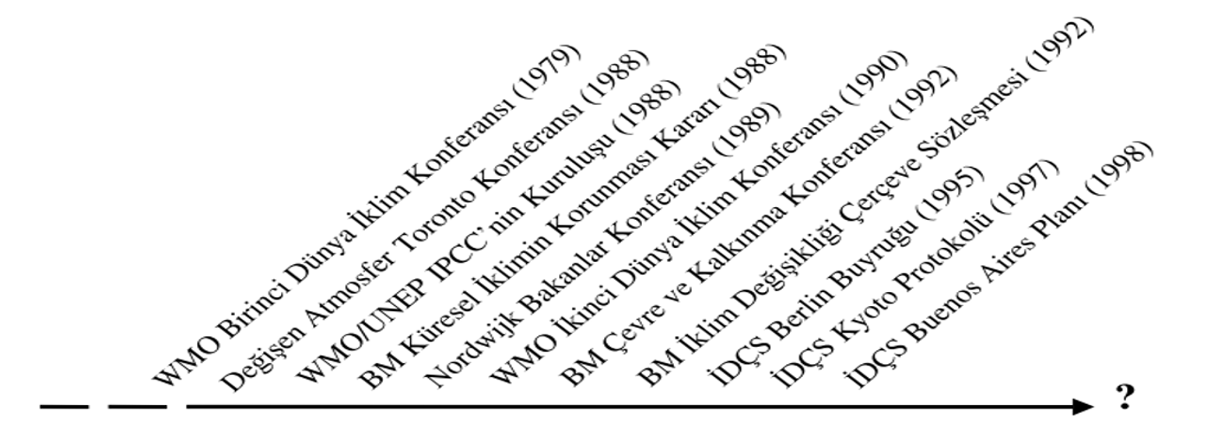
\includegraphics[width=0.95\linewidth,height=0.95\textheight]{tablolar-sekiller/sekil-2-2} \caption{Kaynak: (Mavimbela ve diğerleri, 2018: 42)}\label{fig:unnamed-chunk-2}
\end{figure}

Kaynak: (Türkeş, Sümer ve Çetiner, 2000)

Aşağıda (Tablo 2.1) 1979-2010 yılları arasında iklim kriziyle mücadele etmek için yapılan anlaşmalar derlenmiştir (Çetintaş ve Türköz, 2017). Bunlara, ek olarak 2010 sonrasında yapılan anlaşmalar da eklenmiştir.

\textbf{Tablo 2.1:} Uluslararası İklim Değişikliği Müzakerelerinin Süreci.

\begin{figure}
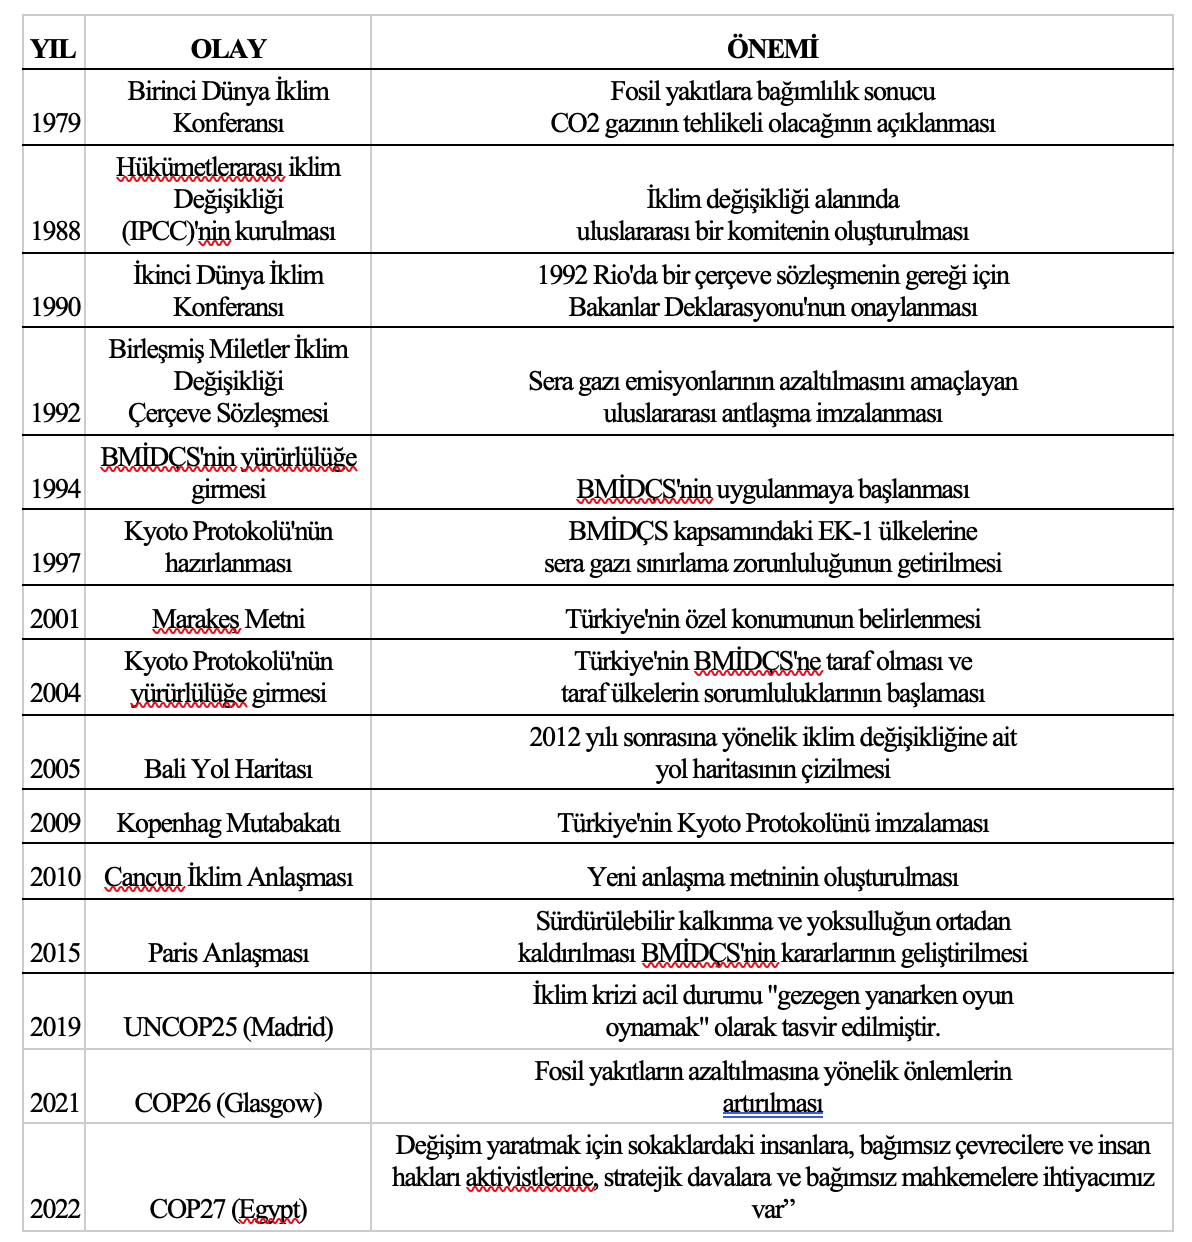
\includegraphics[width=0.95\linewidth,height=0.95\textheight]{tablolar-sekiller/tablo-2-1} \caption{Kaynak: (Mavimbela ve diğerleri, 2018: 42)}\label{fig:unnamed-chunk-3}
\end{figure}

YIL OLAY ÖNEMİ
1979 Birinci Dünya İklim Konferansı Fosil yakıtlara bağımlılık sonucu
CO2 gazının tehlikeli olacağının açıklanması
1988 Hükümetlerarası iklim Değişikliği
(IPCC)'nin kurulması İklim değişikliği alanında
uluslararası bir komitenin oluşturulması
1990 İkinci Dünya İklim Konferansı 1992 Rio'da bir çerçeve sözleşmenin gereği için
Bakanlar Deklarasyonu'nun onaylanması
1992 Birleşmiş Miletler İklim Değişikliği
Çerçeve Sözleşmesi Sera gazı emisyonlarının azaltılmasını amaçlayan
uluslararası antlaşma imzalanması
1994 BMİDÇS'nin yürürlülüğe girmesi BMİDÇS'nin uygulanmaya başlanması
1997 Kyoto Protokolü'nün hazırlanması BMİDÇS kapsamındaki EK-1 ülkelerine
sera gazı sınırlama zorunluluğunun getirilmesi
2001 Marakeş Metni Türkiye'nin özel konumunun belirlenmesi
2004 Kyoto Protokolü'nün yürürlülüğe girmesi Türkiye'nin BMİDÇS'ne taraf olması ve
taraf ülkelerin sorumluluklarının başlaması
2005 Bali Yol Haritası 2012 yılı sonrasına yönelik iklim değişikliğine ait
yol haritasının çizilmesi
2009 Kopenhag Mutabakatı Türkiye'nin Kyoto Protokolünü imzalaması
2010 Cancun İklim Anlaşması Yeni anlaşma metninin oluşturulması
2015 Paris Anlaşması Sürdürülebilir kalkınma ve yoksulluğun ortadan
kaldırılması BMİDÇS'nin kararlarının geliştirilmesi
2019 UNCOP25 (Madrid) İklim krizi acil durumu ``gezegen yanarken oyun
oynamak'' olarak tasvir edilmiştir.
2021 COP26 (Glasgow) Fosil yakıtların azaltılmasına yönelik önlemlerin
artırılması
2022 COP27 (Egypt) Değişim yaratmak için sokaklardaki insanlara, bağımsız çevrecilere ve insan hakları aktivistlerine, stratejik davalara ve bağımsız mahkemelere ihtiyacımız var''

\textbf{Kaynak:} (Çetintaş ve Türköz, 2017; ``United Nations Climate Change Conference,Wikipedia'', 2022.)

Kyoto Protokolü, karbon dioksit ve sera etkisine neden olan diğer 5 gazın salınımını azaltmayı yasal yükümlülüklere bağlamış; 1997 yılında Japonya'nın Kyoto şehrinde imzalanmış ve 2005 Şubat'ında yürürlüğe girmiştir. Türkiye ise bu protokole 2009 yılında katılmıştır. Türkiye Dışişleri Bakanlığı sayfasındaki verilere göre Kyoto Protokolünde 191 ülke ve AB yer almaktadır (Kyoto Protokolü). \citep{kyoto2019kyoto}

Özet olarak; Birinci Dünya İklim Değişikliği Konferansı, Cenevre'de 1979 yılında toplanmıştı. Uluslararası İklim Değişikliği Paneli, 1988'de kurulmuştu. Kyoto Protokolü (1997), iklim değişikliğinin azaltılmasına ilişkin ilk uluslararası anlaşmadır. Bugüne kadarki en kapsamlı anlaşma, 2015 yılında Paris'te COP21'de imzalanmıştır. İklim krizinin anlaşılmasına yönelik olarak birçok IPCC raporu yayımlanmaktadır. Yıllar boyunca bu uygulamalar kapsamında kendini gösteren iklim krizi acil eyleme dönüşmüştür. BM'nin bünyesinde gerçekleştirilen ardışık bir uluslararası konferanstan yapıcı bir sonuç çıkmamasına rağmen doğa bilimcileri kendi ilan ettikleri iklim acil durumunu, ahlaki yükümlülük ve insanlığa gerekli katkı olarak tanımlamaktadır. Eğer sistem bu şekilde ilerler ve gerekli önlemler alınmazsa dünyanın kesinlikle yaşanılmaz bir hale geleceği vurgulanmaktadır (s. 14).\citep{harvey2016climate}

İklim acil durumu, apolitik, ekonomik, toplumsal ve kültürel açılardan da bir acil durumdur. 2019 yılında Madrid'de düzenlenen UNCOP25 konferansı, bu acil durumu ``gezegen yanarken oyun oynamak'' olarak tasvir etmiştir. Amazon ormanlarının büyük arazilerinin siyasi lisansla yakılmasından sonra, Avustralya'da eşi görülmemiş büyüklükte orman yangınları çıkmıştır (Harvey, 2016, UNCOP25: 16). \citep{harvey2016climate} Son yıllarda, ülkemizde de iklim krizi kaynaklı birçok orman yangını görülmektedir. 15 Aralık 2018 tarihinde, Polonya'nın Katowice kasabasında 200 ülkenin diplomatları, sera gazı emisyonlarını azaltmak için Birleşmiş Milletler İklim Değişikliği Çerçeve Sözleşmesi kapsamında hazırlanan Paris Anlaşması'nı desteklemek ve uygulamak için bir araya geldi. Bu anlaşmanın amacı, ülkelerin belirli standartlar ölçüsünde gaz emisyonlarını izlemesini ve iklim politikalarını uygulamasını sağlamaktır. İklim krizi tek başına ulusal hükümetler tarafından çözülemeyecek kadar karmaşık bir sorundur. Bireylerden iş dünyasına kadar her kişi ve kuruma büyük sorumluluklar düşmektedir. \citep{dhanda2019climate} 2021 yılında Ege, Akdeniz, Batı Karadeniz, Güneydoğu Anadolu bölgelerinde çok büyük boyutlu orman yangıları görülmüştür. 59 ilde 299 orman yangını yaşanmıştır. Yüzbinlerce hektar orman ve yerleşim yeri küle dönmüş ve yüzbinlerce hayvan can vermiştir (Vikipedi, 2021). Gerekli önlemlerin alınmaması bu yangınların haftalarca sürmesine neden olmuştur.

İklim değişikliği çalışmalarından ortaya çıkan endişeler şu şekildedir (s. 3-4): \citep{pink2018climate}

\textbf{Tehlike:} Can kaybı, yaralanma veya diğer sağlık etkilerinin yanı sıra mülk, altyapı, geçim kaynakları, hizmet sunumunda hasar ve kayıplara neden olabilecek doğal veya insan kaynaklı fiziksel olaylar. Ekosistemler ve çevresel kaynakların zarar görmesi.

\textbf{Maruz kalma:} Olumsuz etkilenebilecek yer ve ortamlarda insanların, geçim kaynaklarının, türlerin veya ekosistemlerin, çevresel işlevlerin, hizmetlerin ve kaynakların, altyapının veya ekonomik, sosyal veya kültürel varlığının tehlikeye maruz kalması.

\textbf{Hasar görülebilirlik -- kırılganlık:} Olumsuz etkilenme eğilimi ve yakınlığı ifade etmektedir. Güvenlik açığına, zarara duyarlılık ya da yatkınlık gibi durumlarla başa çıkma ve uyum sağlama kapasitesinin olmaması gibi çeşitli kavramları ve unsurları kapsar.

\textbf{Etkiler:} Doğal ve beşerî sistemler üzerindeki etkiler tanımlanmaktadır. İklim değişikliğinin sel, kuraklık ve deniz seviyesinin yükselmesi dâhil olmak üzere jeofizik sistemler üzerindeki etkileri, fiziksel etkiler olarak adlandırılan etkilerin bir alt kümesini ifade eder.

\textbf{Risk:} Değerlerin çeşitliliğini kabul ederek değerli bir şeyin tehlikede olduğu ve sonucun belirsiz olduğu durumlarda sonuçların potansiyelini tasvir eder. Genellikle risk, tehlikeli olayların veya eğilimlerin meydana gelme olasılığıyla bu olayların veya eğilimlerin meydana gelmesi durumunda olası etkilerle çarpımı olarak temsil edilir.

\textbf{Adaptasyon:} Gerçek veya beklenen iklime ve onun etkilerine uyum sürecine uyumu tanımlar. İnsan sistemlerinde uyum, zararı azaltmayı, önlemeyi veya fırsatlardan yararlanmayı amaçlar.

\textbf{Dayanıklılık:} Sosyal, ekonomik ve çevresel sistemlerin tehlikeli bir olay, eğilim veya rahatsızlıkla başa çıkmayı ifade etmektedir. Bu sistemlerin temel işlevlerini, kimliklerini ve yapılarını sürdürecek şekilde yanıt verme veya yeniden düzenleme, aynı zamanda uyum, öğrenme ve dönüşüm kapasitelerini tanımlar.

\hypertarget{iklim-deux11fiux15fikliux11finin-etkileri-ve-sonuuxe7larux131}{%
\section{İklim Değişikliğinin Etkileri ve Sonuçları}\label{iklim-deux11fiux15fikliux11finin-etkileri-ve-sonuuxe7larux131}}

İklim değişikliğinin etkileri ve sonuçları çok katmanlı bir yapıdan oluşmaktadır. Sıcaklıkların artması, doğal afetler, buzulların erimesi, mercan resifleri ve okyanusların tuzluluğunun artması, hava kirliliği, su kirliliği, yaşam süresinin uzaması, ilaçlama, biyolojik çeşitlilik bu katmanlardan bazılarını oluşturmaktadır. İklim değişikliğinin etki ve sonuçlarını daha iyi anlayabilmek adına bu başlıklara kısa bir şekilde değinmek önem arz etmektedir.

\hypertarget{sux131caklux131klarux131n-artmasux131-sux131cak-hava-dalgalarux131}{%
\subsection{Sıcaklıkların Artması -- Sıcak Hava Dalgaları}\label{sux131caklux131klarux131n-artmasux131-sux131cak-hava-dalgalarux131}}

İklim krizinin ülkeleri yalnızca ısınma yoluyla değil, aynı zamanda aşırı sıcak hava dalgalarının daha sık görülmesi yoluyla da etkilemesi muhtemeldir. Miller ve arkadaşlarının yapmış olduğu çalışma bulgularına göre; bu yüzyılın sonuna doğru sadece ortalama sıcaklık değerlerine odaklanılarak tarımdaki iklim hasarlarının tahmin edilenden 5-10 kat daha büyük olabileceğini göstermektedir. Sıcak hava dalgalarının tarım sektöründe kişi başına düşen ekonomik çıktıyı azalttığı, uzun süreli şiddetli sıcak hava dalgalarının tarım dışı çıktıları da etkilediği tespit edilmiştir. \citep{miller2021heat}

Isı dalgaları sıcaklığın normalden daha sıcak olması değil, sıcaklığın birkaç gün devam etmesi, geceleri sıcaklığın neredeyse hiç düşmemesi, ısı yüksekliğinin insanlar için dayanılmaza yakın bir hal alması gibi durumları tarif etmektedir. Isı dalgaları bilim insanlarının iklim değişikliği ve küresel ısınma hakkında endişelenmeye başlamasından bu yana aniden ortaya çıkmamıştır. İlk belgelenmiş vaka, 1858 tarihinde Londra'nın üzerine çöken aşırı sıcaklık gösterilmektedir. Thames Nehri, iki milyondan fazla insanın atıklarını denize taşıyan bir lağım görevi görmekteydi. Gel-gitlerden dolayı atıkların çoğu geri gelmekteydi. Koku yaz sıcağında dayanılmaz boyutlara gelmişti. İçme suyu, şehir dışındaki yeraltı su kaynaklarından geldiğinden ve aynı zamanda insan atıkları tarafından kirlendiği için kolera da sürekli bir tehdit haline gelmişti (s. 2). \citep{bush2020}

\hypertarget{doux11fal-afetler}{%
\subsection{Doğal Afetler}\label{doux11fal-afetler}}

1996'dan 2015'e kadar olan süreçte, Belçika'nın Brüksel kentindeki Louvain Katolik Üniversitesi'ne bağlı Afetlerin Epidemiyolojisi Araştırma Merkezi (CRED) tarafından sağlanan veri tabanına göre, 7000'den fazla afet görülmüştür. Depremler, tsunamiler ve volkanik patlamalar gibi jeofizik afetlerin sıklığı hemen hemen aynı kalırken, sel, fırtına, sıcak hava dalgaları gibi iklim ve hava koşullarıyla ilgili olaylarda sürekli bir artış olduğu gözlemlenmiştir (s. 6). \citep{bush2020}

\textbf{Şekil 2.3:} Afet Türü Başına Ölüm Sayısı.

\begin{figure}
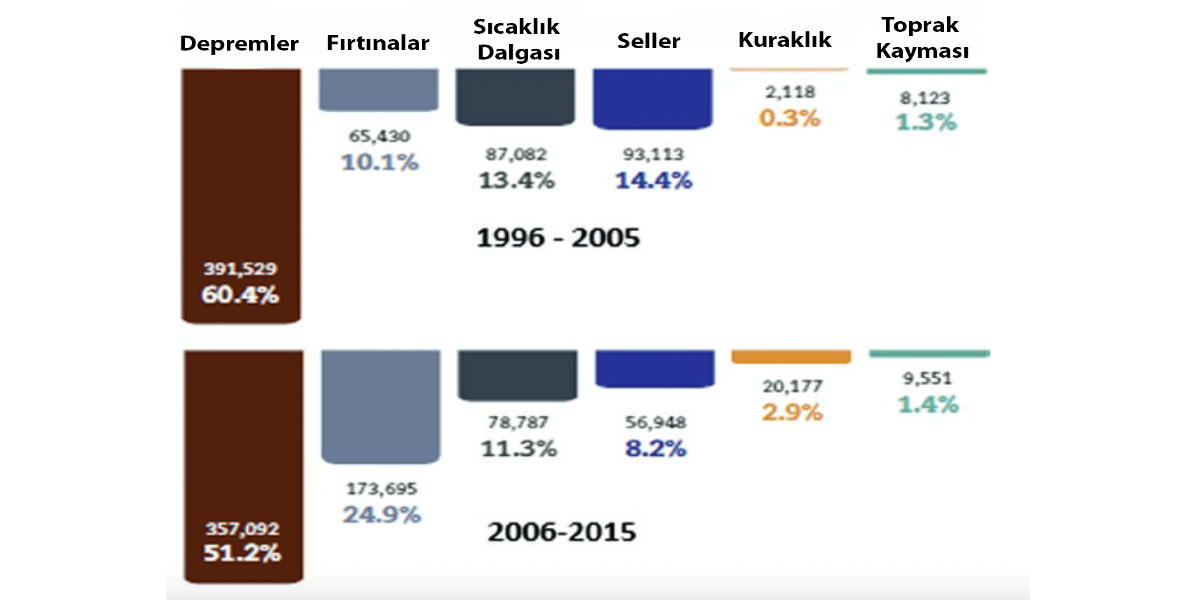
\includegraphics[width=0.95\linewidth,height=0.95\textheight]{tablolar-sekiller/sekil-2-3} \caption{Kaynak: (“Poverty & Death: Disaster and Mortality 1996-2015 World | ReliefWeb”)}\label{fig:unnamed-chunk-4}
\end{figure}

\hypertarget{buzullarux131n-erimesi}{%
\subsection{Buzulların Erimesi}\label{buzullarux131n-erimesi}}

Bush kitabında, buzulların erimesini deniz buzu, buzullar, deniz örtüsü, donmuş toprak olarak dört katmanda açıklamaktadır. Cryosphere olarak adlandırılan deniz buzu, buzullar, deniz örtüsü ve donmuş zemini içermektedir. Bu soğuk oluşumlar çok yüksek derecede donmuş su tutmaktadır. Bu buzulların erimesi, küresel deniz seviyesinin yükselmesi anlamına gelmektedir. Bu da birçok felaketi beraberinde getirecektir. \citep{bush2020}

\hypertarget{deniz-buzu}{%
\subsubsection{Deniz Buzu}\label{deniz-buzu}}

Deniz buzu, okyanus yüzeyinde yüzen donmuş deniz suyudur. Gezegenin her iki ucunda milyonlarca kilometrekarelik bir alanı kaplayan deniz buzu, donar ve ardından kutup mevsimleriyle birlikte erimektedir. İnsan faaliyetlerinin ve ekosistem habitatlarının mevsimsel ritimlerinin koreografisini oluşturur. Kuzey kutbunda, bazı deniz buzu yıldan yıla varlığını sürdürürken, güney okyanusu / Antarktika'da deniz buzu daha mevsimseldir. Bazı zamanlar tamamen erimekte ve her yıl yeniden oluşmaktadır. Bu her iki kutup bölgesindeki kara ve deniz memelilerinin yaşam alanları için hayati önem taşımaktadır (s. 16). \citep{bush2020}

\hypertarget{buzullar}{%
\subsubsection{Buzullar}\label{buzullar}}

1960'ların başından beri, yaklaşık 40 buzul için sürekli kütle dengesi kayıtları tutulmaktadır. Bu veriler, dünyanın çoğu bölgesinde buzulların boyutlarının küçüldüğünü göstermektedir. 1961'den 2005'e kadar birçok küçük buzulun kalınlığı yaklaşık 12 metre veya 9000 kilometreküp suya eşdeğer azalmıştır (SOTC).
Dünya Buzulu İzleme Servisi'nden (WGMS) gözlemsel veri setleri üzerinde yapılan bir araştırmada ``21. yüzyılın başlarındaki kütle kaybı oranlarının küresel ölçekte, en azından gözlemlenen zaman periyodu ve muhtemelen aynı zamanda kayıtlı tarih için emsali olmadığı'' sonucuna varmıştır (s. 18). \citep{bush2020}

\hypertarget{buz-uxf6rtuxfcsuxfc}{%
\subsubsection{Buz Örtüsü}\label{buz-uxf6rtuxfcsuxfc}}

Buz alanı 50.000 km2'den fazla ise, buz tabakası olarak tanımlanmaktadır. Son buzul çağlarında, kuzey yarımkürenin çoğunu buz tabakaları kaplamış olsa da gezegende şu anda sadece iki büyük buz tabakası bulunmaktadır: Bu buz tabakalarının biri Grönland'da, diğeri Antarktika'dadır. Grönland buz tabakası, tabakaların ikisinden daha küçük olanıdır: yaklaşık 1,7 milyon km2'yi kaplar. Buna karşın, Antarktika buz tabakasının alanı çok daha büyüktür ve yaklaşık 14 milyon km2'dir. Bu, kıta ABD'sinin alanının bir buçuk katından fazladır (s. 19-20). \citep{bush2020}

\hypertarget{donmuux15f-toprak-permafrost}{%
\subsubsection{Donmuş Toprak-Permafrost}\label{donmuux15f-toprak-permafrost}}

Permafrost ya da kalıcı olarak donmuş zemin, en az iki yıl boyunca 0 °C'de kalan toprak, tortu veya kayalardan oluşmaktadır. Adına rağmen, permafrost, kalıcılığından çok istikrarsızlığıyla karakterize edilir. `Aktif katman kalınlığı' veya ALT olarak adlandırılan katman, mevsimsel döngü boyunca eriyen ve donan katmandır ve daha sıcak koşullarda daha da büyümektedir. Permafrost, son 2-3 yılda ısınmıştır ve kuzey kutbu boyunca ısınmaya devam etmektedir. Kuzey yarımkürenin kara yüzeyinin yaklaşık \%55'i, mevsimsel olarak donmuş topraklarla kaplıdır; bu, yüksek enlemlerde ve yüksek rakımlarda birkaç ay donmuş halde kalabilmektedir (s. 22). \citep{bush2020}

Büyük miktarlarda organik karbon, kutup bölgelerindeki donmuş topraklarda (permafrost) depolanır. Isınan iklim organik karbonun mikrobiyal parçalanmasına ve sera gazlarının karbondioksit ve metan salınımını hızlandıran çevresel değişikliklere neden olabilmektedir. Bu geri bildirim, iklim değişikliğini hızlandırabilir. Ancak bu bölgelerden kaynaklanan sera gazı emisyonunun büyüklüğü, zamanlaması ve bunların iklim değişikliği üzerindeki etkisi belirsizliğini korumaktadır. \citep{schuur2015climate}

\hypertarget{mercan-resifleri-ve-okyanuslar}{%
\subsection{Mercan Resifleri ve Okyanuslar}\label{mercan-resifleri-ve-okyanuslar}}

Mercan resifleri, dünyanın herhangi bir yerinde var olan en üretken ve biyolojik olarak en zengin ekosistemlerden biridir. Balıklar, süngerler, kestaneler, kabuklular ve yumuşakçalar dâhil olmak üzere bilinen tüm deniz türlerinin kabaca dörtte biri için temel yaşam alanıdır. Ayrıca, dünya çapında kıyı topluluklarında yaşayan birkaç yüz milyon insan için temel ekosistem hizmetleri sağlamaktadır. Gelişmekte olan ülkelerdeki birçok kıyı topluluğunun geçimi, mercan resifleri arasında toplanıp gelişen balıklara bağlıdır. Bu geçim kaynakları, artık dünya resiflerinin kötüleşen durumu tarafından tehdit edilmektedir. 2011'de, Dünya Kaynakları Enstitüsü, dünya mercan resiflerinin durumunu ve bunlara yönelik tehditleri araştıran 2005'te yürüttüğü çalışmalarını yeniden gözden geçirdi. Enstitünün temel bulguları aşağıda sıralanmıştır (s. 22-23). \citep{bush2020}

• Dünya resiflerinin \%60'ından fazlası, aşırı avlanma ve yıkıcı balıkçılık faaliyetleri, kıyı gelişimi, su havzası kaynaklı kirlilik veya deniz kaynaklı kirlilik ve hasar gibi bir veya daha fazla yerel kaynaktan dolaylı ve doğrudan tehdit altındadır.

• Mercan resifleri üzerindeki yerel baskılar arasında aşırı avlanma, yıkıcı balık avları, dünya resiflerinin \%55'inden fazlasını etkileyen en yaygın acil tehdittir. Kıyı gelişimi ve havza kaynaklı kirlilik, her biri resiflerin yaklaşık \%25'ini tehdit etmektedir. Deniz kaynaklı kirlilik ve gemilerden kaynaklanan hasar, yaygındır ve resiflerin yaklaşık \%10'unu tehdit etmektedir.

• Dünyadaki mercan resiflerinin yaklaşık \%75'i, yerel tehditler termal stres ile birleştiğinde tehdit altında olarak derecelendirilir. Bu, artan okyanus sıcaklıklarının son zamanlardaki etkilerini yansıtır, aynı zamanda mercanların kitlesel mercan ağartmasına bağlı olarak yaygın şekilde zayıflaması ve ölümüyle bağlantılıdır.

Hoegh-Guldberg ve arkadaşlarının mercan resifleriyle ilişkili balıkçılık, turizm, kıyı koruma ve insanlar için giderek daha ciddi sonuçları öngören mercan resifleri için gelecek senaryoların değerlendirdikleri çalışmada, atmosferdeki karbondioksit konsantrasyonunun milyonda 500 parçayı aşması ve küresel sıcaklıkların 2050 ile 2100 arasında en az 2°C artmasının beklendiğini belirtmişlerdir Bu değerler mevcut deniz organizmalarının çoğunun evrimleştiği dönemin, en azından son 420.000 yılın değerlerini önemli ölçüde aşmaktadır. 21. yüzyılda beklenen koşullar altında, küresel ısınma ve okyanus asitlenmesi, mercanların resif sistemlerinde giderek daha nadir hale gelmesiyle birlikte, karbonat birikimini tehlikeye atmaktadır. Sonuç, daha az çeşitli resif toplulukları ve bakımı yapılamayan karbonat resif yapıları olacaktır. İklim değişikliği aynı zamanda, azalan su kalitesinden ve önemli türlerin aşırı kullanımından kaynaklanan yerel stresleri şiddetlendirerek resifleri giderek işlevsel çöküşün devrilme noktasına doğru itmektedir. Mercanların baskın olduğu ekosistemlerin kaybından kaçınılması için ölçeklendirilmiş yönetim müdahalesi ve küresel emisyonlar üzerinde kararlı eylemler gerekmektedir. \citep{hoegh2007coral}

\hypertarget{asitleux15fme}{%
\subsection{Asitleşme}\label{asitleux15fme}}

Okyanus suyunun kimyası, birçok deniz kabuklu türü üzerinde ölümcül etkisi olabilecek şekillerde değişmektedir. Okyanus asitlenmesi, deniz suyunda çeşitli kimyasal değişikliklere neden olmaktadır. Atmosferdeki karbondioksit, suda çözünerek karbonik asit oluşturmaktadır. Son 150 yılda okyanus yüzey suları, atmosferden büyük miktarlarda CO2 emdiği için \%30 daha asidik hale geldi. Endüstri öncesi dönemden bu yana okyanuslar, atmosfere salınan CO2'nin çoğunu absorbe etmiştir, halen devam etmekte olan bir absorpsiyona sahiptir (s. 25). \citep{bush2020}

\hypertarget{oksijensizleux15ftirme}{%
\subsection{Oksijensizleştirme}\label{oksijensizleux15ftirme}}

Oksijen, mikroplardan balinalara kadar okyanustaki neredeyse tüm yaşam için gereklidir. Ancak son birkaç yılda okyanus ısınmasıyla bağlantılı iklim kaynaklı oksijen kaybının (deoksijenasyon) dünyanın tüm bölgelerinde giderek daha belirgin hale gelmiştir. Çözünmüş oksijen seviyelerinin neredeyse sıfıra düşmesiyle (hipoksi) deniz türleri hayatta kalamamaktadır. Etkilenen bölgeye ``ölü bölge'' denmektedir. Küresel okyanus oksijensizleşmesi, artan okyanus sıcaklıklarının doğrudan bir etkisidir. Okyanusların ısınması, oksijenin çözünürlüğünü azaltmaktadır (daha sıcak su daha az oksijen tutmaktadır). Okyanuslardaki oksijenin yükselmesi ve dolaşımı yoluyla, fiziksel karışım değişmektedir. Ayrıca, daha sıcak sular deniz canlılarının metabolizmasını artırarak, oksijen ihtiyaçlarını da artırmaktadır (s. 26). \citep{bush2020}

\hypertarget{plastik-kirliliux11fi}{%
\subsection{Plastik Kirliliği}\label{plastik-kirliliux11fi}}

6 milyardan fazla insan tarafından tüketilen plastik atık miktarı yılda yaklaşık 300 milyon tonu bulmaktadır. Bu plastiğin çoğu dönüştürülebilseydi, çevresel etki belki de yönetilebilir olabilirdi. Bu plastik atıklar hem deniz türleri hem de deniz kuşları üzerinde giderek daha fazla ölümcül bir hale gelmektedir (s. 27). \citep{bush2020}

\hypertarget{hava-kirliliux11fi}{%
\subsection{Hava Kirliliği}\label{hava-kirliliux11fi}}

Kirlilik, bugün dünyadaki hastalıkların ve erken ölümlerin en büyük çevresel nedenidir. Kirliliğin neden olduğu hastalıklar, 2015 yılında tahmini 9 milyon erken ölümden sorumludur. Dünya çapındaki tüm ölümlerin \%16'sı; AIDS, tüberküloz ve sıtmadan üç kat daha fazla ölüm ve tüm savaşlardan diğer şiddet biçimlerinden 15 kat daha fazladır. En ciddi şekilde etkilenen ülkelerde; hava kirliliğinin sebep olduğu ölümler, tüm ölüm oranlarının dörtte birinden fazladır (s. 1). \citep{landrigan2018lancet}

Kirlilik; şu anda milyonlarca insanın sağlığını tehlikeye atan, dünyanın ekosistemlerini bozan, ulusların ekonomik güvenliğini baltalayan ve hastalıklardan, sakatlıklardan ve erken ölümden sorumlu olan önemli bir küresel sorundur. Daha önce tanınandan çok daha geniş bir hastalık yelpazesi ile ilişkilidir. Hava kirliliği, astım, kanser, nöro gelişimsel bozukluklar ve çocuklarda doğum kusurları dâhil birçok bulaşıcı olmayan hastalığın önemli bir etkeni olduğu anlaşılmaktadır. Yetişkinlerde ise, kalp hastalığı, felç, kronik obstrüktif akciğer rahatsızlığı ve kanser gibi hastalıklara neden olmaktadır (akt. Bush: 32; Landrigan ve diğerleri, 2018). \citep[akt][]{bush2020, landrigan2018lancet}

\begin{enumerate}
\def\labelenumi{\arabic{enumi})}
\tightlist
\item
  Dış Hava Kirliliği
  İklimdeki son değişiklikler, özellikle sıcaklık artışları, dünyanın birçok yerinde çeşitli fiziksel ve biyolojik sistemleri hâlihazırda etkilediğini göstermektedir. Alerjen kalıpları da iklim değişikliğine bağlı olarak değişmektedir. Hava kirliliği, özellikle belirli hava koşullarının varlığında polen tanelerinin alerjenik potansiyelini değiştirebilir. Geçen yüzyılda; ekonomik ve endüstriyel büyümeye bağlı olarak hava kirliliğindeki büyük artış, çok sayıda Avrupa ve Kuzey Amerika ülkelerinde birinci dereceden çevre sorunlarına yol açtı. Hava kirliliği, şu anda dünyanın diğer bölgelerinde de ortaya çıkan bir sorundur. \citep{damato2014climate}
\end{enumerate}

Dünya Sağlık Örgütü, 2016 yılında, dış hava kirliliğiyle ilgili kapsamlı bir çalışma yayımlamıştır. Yaklaşık 3.000 şehir ve kasabada, 540.000 kişiden veri toplanmıştır. Hava kalitesinin bir göstergesi olarak, partikül seviyeleri incelenmiştir. Partikül maddeler, erken ölümle sonuçlanabilecek çok çeşitli tıbbi durumlardan sorumlu olan zararlı bir kirleticidir (s. 32-33). \citep{bush2020}

\begin{enumerate}
\def\labelenumi{\arabic{enumi})}
\setcounter{enumi}{1}
\tightlist
\item
  Evsel Hava Kirliliği
  Hava kirliliği ve bununla bağlantılı sağlık etkileri, küresel bir endişe kaynağıdır. Evsel hava kirliliği, iklim değişikliği ve temiz pişirme yakıtlarına erişim konularındaki mevcut politikalar hem dış mekân hem de ev içi hava kirliliğinin etkili bir şekilde nasıl azaltabileceğini ve insan sağlığını nasıl iyileştirebileceğini ele almaktadır. \citep{rao2013better}
\end{enumerate}

Katı ev yakıtlarının kullanımından kaynaklanan hava kirliliği, artık gelişmekte olan ülkelerde de önemli bir sağlık riski olarak kabul edilmektedir. Buna göre, kalkınma düşüncesinde ve yatırımda, yalnızca hanelerde tüketilen yakıt kullanımının verimliliğini artırmaya odaklanan çabalardan çevre ve insan sağlığını önceleyerek hava kirliliğine maruz kalmayı azaltmaya odaklanan çabalara doğru bir miktar kayma olmuştur. Ancak ne yazık ki bu tam olarak, iklim gündeminin uluslararası sürdürülebilir kalkınma konusundaki söylem ve eylemlerinin çoğuna hâkim hale gelmesiyle gerçekleşebilmektedir. Bu nedenle, merkezi olarak büyük sağlık etkisine odaklanan yaklaşımları optimize etmek yerine, hane halkı enerji gündemi de sürdürülebilirlik tanımının dayattığı kısıtlamalar tarafından engellenmiştir. \citep{goldemberg2018household}

\begin{enumerate}
\def\labelenumi{\arabic{enumi})}
\setcounter{enumi}{2}
\tightlist
\item
  Hava Kirliliği ve Çocuk
  Hava kirliliği, her yıl beş yaşın altındaki yaklaşık 650.000 çocuğu öldüren hastalık ve enfeksiyonlarla doğrudan bağlantılıdır. Her yıl yaklaşık bir milyon çocuk zatürreden ölmektedir ve bu ölümlere sebep olan bu hastalığın yarısından fazlasına doğrudan hava kirliliği sebep olmaktadır. Buna göre hava kirliliği; zatürre, bronşit ve astım gibi solunum yolu rahatsızlıkları ile güçlü bir şekilde ilişkilidir. Ülkelerin sanayileşmesi ve kentleşmesi arttıkça enerji kullanımı da artmaktadır. Bu enerji kullanımı kömür ve karbon yakıtlarından oluşuyorsa hava kirliliği önemli ölçüde kötüleşmektedir. Çocuklar, özellikle hava kaynaklı kirleticilere karşı hassastır. Solunum yollarının iç kısmındaki hücre tabakası çocuklarda daha geçirgendir ve çocukların solunum yolları yetişkinlere göre daha küçüktür. Enfeksiyonların tıkanıklığa neden olma olasılığı daha yüksektir. Çocuklar ayrıca yetişkinlere kıyasla vücut ağırlığının birimi başına daha fazla hava soluyarak iki kat daha hızlı nefes alırlar. Hava kirliliği yüksek bir ortamda yaşayan çocukların akciğer kapasitesi, pasif olarak sigara dumanına maruz kalan çocuklarda olduğu gibi \%20 oranında azalabilir (s. 37-38). \citep{bush2020}
\end{enumerate}

\hypertarget{su-kirliliux11fi}{%
\subsection{Su Kirliliği}\label{su-kirliliux11fi}}

Su kaynakları, sadece insanlar için değil özünde tüm ekosistemler için hayati öneme sahiptir. İçme suyunun kirlenmesi insan sağlığını riske atmaktadır. Su; aynı zamanda tarım, imalat, enerji üretimi ve diğer çeşitli kullanımlar için de gereklidir. İklim değişikliği su mevcudiyetini azaltırken artan sıcaklıklar ve buharlaşma sonucu artan su talebine neden olabilir. Öte yandan, iklim değişikliğinin bir sonucu olarak ortaya çıkan aşırı olaylar, yüzey akışını ve taşkınları artırarak su kalitesini de bozabilir. Bu nedenle değişen iklim ve onun olası etkileri, su kaynakları üzerinde daha fazla baskı oluşturmaktadır. Suda azot ve fosfor gibi yüksek konsantrasyonlarda besin bulunduğunda meydana gelen su ötrofikasyonudur. Besinler; tarım, atık su, yağmur suyu ve fosil yakıt yanması gibi farklı kaynaklardan gelir. Alg patlamaları, oksijensizleşme ve su toksisitesi gibi birçok soruna neden olabilir; sonuçta normal ekosistem işleyişini bozabilir. \citep{nazari2018climate}

Dünyadaki nehir ve göllerdeki kirlilik seviyesi önemli ölçüde değişmektedir. Gelişmiş ülkelerin çoğunda suyun kalitesi, önemli ölçüde iyileşirken BM Çevre Programı'nın (UNEP) 2016 raporuna göre; Latin Amerika, Afrika ve Asya'daki nehirlerin çoğunda 1990'lardan bu yana su kirliliği kötüleşmiştir. \citep{unep2016snapshot}

\hypertarget{yaux15fam-suxfcresinin-artmasux131}{%
\subsection{Yaşam Süresinin Artması}\label{yaux15fam-suxfcresinin-artmasux131}}

Dünyanın çevre ve iklim açısından yaşadığı sağlık sorunlarının yanı sıra, Antroposen Çağında baskın türlerin sağlığına hızlı bir şekilde bakılması gerektiği belirtilmektedir. İnsanlar daha mı uzun yaşıyordu? İyi sağlıkları var mıydı? Peki ya çocuklar? Küresel olarak 2000 ile 2015 yılları arasında yaşam süresi beklentisinde genel olarak 5,9 yıllık küresel bir artış olmuştur. Ölüme neden olan belirtilerle ilgili yapılan çalışmalar bu önemli kazanımlara katkıda bulunmuştur. Dünya genelinde özellikle düşük ve orta gelirli ülkelerde, Birlemiş Milletler kuruluşlarıyla büyük sivil toplum kuruluşları tarafından yapılan çalışmalar neticesinde yaşam süreleri uzamıştır (s. 40-41). \citep{bush2020}

\hypertarget{ilauxe7lama}{%
\subsection{İlaçlama}\label{ilauxe7lama}}

İlaçlama; insanlar tarafından ürün verimliliği, böcek vektörünün artırılması, hastalıkların kontrol altında tutulması için kullanılan biyolojik kirleticilerdir. Pestisitlerin aşırı kullanımı, insanlar da dâhil olmak üzere organizmalar için ciddi yaşamsal tehlikelere neden olmaktadır. Aynı zamanda bu aşırı kullanım, biyolojik çeşitliliğin yok olmasına sebep olabilir. Birçok kuş, böcek, suda yaşayan organizmalar ve hayvanlar bu tehlikenin altındadır. \citep{dubey2021climate}

2017'deki bir BM raporu, gıda üzerine yapmış olduğu çalışmada pestisit kullanımını ele almıştır. Rapor, pestisitlerin, yılda yaklaşık 200.000 akut zehirlenme ölümünün sorumlusu olduğunu ve bu vakaların \%99'unun gelişmekte olan ülkelerde meydana geldiğini ortaya koymaktadır. Bazı ülkelerde, pestisit zehirlenmelerinin bulaşıcı hastalıklardan kaynaklanan ölümlerin sayısını aştığı belirtilmiştir (s. 42-43). \citep{bush2020}

\hypertarget{biyouxe7eux15fitlilik}{%
\subsection{Biyoçeşitlilik}\label{biyouxe7eux15fitlilik}}

İklim değişikliği; biyolojik çeşitlilik, ekosistemler için yaygın ve büyüyen küresel bir tehdittir. Bu değişiklik; bireysel türleri, ekosistemlerin yapısını ve işlevini, doğal sistemlerin topluma sağladığı mal ve hizmetleri değiştiren diğer organizmalarla ve habitatlarıyla etkileşim biçimlerini etkilemektedir. Ekolojik tepkilerin yönünü ve büyüklüğünü anlamak, insan topluluklarının bu değişiklikleri daha iyi tahmin etmelerine ve gerektiğinde buna uyum sağlamalarına yardımcı olmaktadır. \citep{weiskopf2020climate}

Bu gezegeni çok farklı canlılarla paylaşıyoruz. İnsanoğlu; çoğunlukla diğer canlıların yaşam alanlarını yok ederek, sularını kirleterek, endüstriyel atıklarla böcek ilaçları ve toksik kimyasallarla onları zehirleyerek ve dahası onları genellikle yok olma noktasına kadar avlayarak, öldürerek ve bunlara benzer birçok kötü eylemlerde bulunarak biyolojik çeşitliliğe zarar vermiştir. Bu durum devam etmektedir: Fillerin dişleri ve gergedanların boynuzları için öldürülmesi (s 43), \citep{bush2020} başka canlılar üzerinden ticari faaliyetlerine devam eden hayvancılık sektörü uygulamaları da bu zararlara verilebilecek örneklerdendir.

2016 yılında yayınlanan bir raporda; primatlar, toynaklılar, yarasalar, keseliler, kemirgenler ve etoburlar dâhil olmak üzere 300'den fazla memeli türünün avlanma tehdidi altında olduğu tespit edilmiştir. Bu hayvanları avlamanın birincil nedeni, insanların tüketmesi için et elde etmektir. Aynı zamanda hayvanlar geleneksel tıp için deney aracı olarak kullanılmakta ve evcil hayvan ticareti içinde süs amaçlı kullanılan birer meta olarak görülmektedir. Küresel biyoçeşitliliğe yönelik tehditler, yalnızca değişen iklimden kaynaklanmamaktadır: Aslında çok daha yeni bir fenomen olan iklim değişikliği, en azından şu an için birçok türü yok olmaya iten diğer baskılardan daha az şiddetlidir. Bu tehditler şunları içerir (s. 43-44): \citep{bush2020}

\begin{enumerate}
\def\labelenumi{\arabic{enumi})}
\item
  Habitat kaybı ve bozulması:
  Sürdürülebilir olmayan tarım, ağaç kesimi, yol yapımları, konutsal ve ticari gelişmeler, enerji üretimi ve madenciliğin neden olduğu tahribatlar; ani ve zararlı bir biçimde doğal habitatın parçalanması, bozulması ve tahrip edilmesi (balıklar için su yolları dâhil) etkisine sahiptir. Asya'daki palmiye yağı tarlaları ve Güney Amerika'daki sığır eti üretimi için ormanların temizlenmesi, bu bölgelerdeki biyolojik çeşitlilik üzerinde büyük bir etkiye sahip olmaya devam etmektedir.
\item
  Aşırı sömürü: Sürdürülemez avcılık, balıkçılık, kaçak avlanma ve hasat, türleri geri dönüşü olmayan noktaya getirebilir. Dolaylı aşırı kullanım, hedef dışı türlerin kasıtsız olarak öldürülmesiyle meydana gelmektedir (örneğin, hedef dışı avlanma gibi).
\item
  Kirlilik: Ağırlıklı olarak deniz ortamında bir tehdit oluşturur. Petrol sızıntıları, tarımsal atıklar ve okyanuslardaki büyük miktarlardaki plastik çöpler balıklar ve deniz memelileri üzerinde zararlı ve çoğu zaman ölümcül etkilere sahiptir. Pestisitler, arılar gibi temel tozlayıcı türler üzerinde ciddi bir etkiye sahiptir.
\item
  İstilacı türler ve hastalıklar: İstilacı türler, yiyecek ve habitat için rekabet ederler. Hem yerli türleri avlayabilir hem de daha önce çevrede olmayan ve yerli popülasyonları yok eden hastalıkları getirebilirler.
\end{enumerate}

Ancak iklim değişikliği, yukarıda açıklanan risklere hâlihazırda maruz kalmış çok sayıda tür için ortaya çıkan ve potansiyel tehdit olan varoluşsal bir tehlikedir. Artan sıcaklıklar; birçok türün menzillerini değiştirip iklimin daha uygun olduğu bölgelere taşınmasına neden olacaktır. Örneğin, kelebekler birçok ülkede kutuplara doğru hareket ediyor gibi görünüyor. Ancak birçok tür için bu tür bir adaptasyon mümkün olmayacaktır. Örneğin, Kuzey Kutbu'ndaki kutup ayısı gibi kutup bölgelerinde yaşayan türlerin gidecek başka yerleri yoktur. Bu ikonik tür için gelecek çok kasvetli görünmektedir. Deniz seviyesindeki değişiklikler, alçak adalarda yaşayan veya alçak rakımlı kıyı bölgelerinde yaşayan türler için açık bir tehdit oluşturur. Sadece insan kaynaklı iklim değişikliğinin neden olduğu bir yok oluşun ilk örneği olarak; Büyük Bariyer Resifi'nin doğusundaki Torres Boğazı'ndaki küçük bir adada yaşayan Bramble Cay Melomys adlı küçük bir kemirgen, 2016 yılında adadan kayboldu. Melomys zaten son derece savunmasızdı: Avustralya memelileri arasında en izole ve kısıtlı menzile sahipti (s. 44). \citep{bush2020}

İklim değişikliğinin biyolojik çeşitlilik üzerindeki etkisini tahmin etmek için birkaç model geliştirilmiştir. Bu modellerden elde edilen sonuçlar, iklim değişikliğinin biyoçeşitlilik için bazı endişe verici sonuçlarını ortaya koymaktadır. Örneğin, gelecek yüzyılda birçok bitki ve hayvanın neslinin tükeneceğini, tropik yağmur ormanlarının büyük ölçekli olarak zarar göreceğini ön görmektedir (Willis ve Bhagwat, 2009). \citep{willis2009biodiversity}

Paleontologlar; kitlesel yok oluşları, nispeten kısa bir jeolojik zaman diliminde türlerin çoğunluğunun kaybıyla karakterize edilen olaylar olarak tanımlamaktadır. Son 4-500 milyon yılda, beş kez kitlesel yok oluşlar meydana geldi. Biyoçeşitliliğin sürekli kaybı, türlerin popülasyonlarının azalması ve şu anda yirmi birinci yüzyılda devam etmekte olan türlerin fiili yok oluşlarının sayısı altıncı yok oluş olarak adlandırılmıştır. Geçmişte; yok oluşlar uzun jeolojik zaman dilimlerinde, genellikle milyonlarca yıl boyunca gerçekleşti. İçinde bulunduğumuz çağla ilgili şaşırtıcı olan şey, devam eden kademeli yok oluş sürecinin son derece kısa bir zaman diliminde gerçekleşiyor olmasıdır. Homo sapiens dışında, daha önce hiçbir tek tür gezegen üzerinde bu kadar yıkıcı bir etkiye sahip olmamıştı. Daha önceki yok oluşların tümü, gezegenin değişen ikliminden kaynaklandı. Aradaki fark, değişikliklerin o sırada mevcut olan türlerin üzerinde hiçbir kontrolü olmayan olaylardan kaynaklanmış olmasıdır. Büyük bir meteordan gelen büyük bir darbe, dinozorların saltanatını sona erdirdi. Gezegenin doğal uzun vadeli iklim değişkenliği, çok az hayvan ve bitkinin hayatta kalabileceği kadar şiddetli buzul çağları üretti (s. 45). \citep{bush2020}

\hypertarget{iklim-yuxf6netimini-amaca-uygun-hale-getirecek-uxf6nlemler}{%
\section{İklim Yönetimini Amaca Uygun Hale Getirecek Önlemler}\label{iklim-yuxf6netimini-amaca-uygun-hale-getirecek-uxf6nlemler}}

Demokratik yönetişimin iklim değişikliğinin acil sorununa dikkat çekmesini sağlamanın farklı yolları bulunmaktadır. Ponthieu; gençlik hareketleri, sivil toplum kuruluşları, çevre bilimcileri ve ekonomistlerin iklim değişikliğiyle ilgili söylemleri ve talepleri doğrultusunda 10 maddelik bir iklim acil planı hazırlamıştır. Bu başlığın temel çatısı, Ponthieu'nun ``The Climate Crisis, Democracy and Governance Transition in Ten Steps: Action Points for Goverments'' kitabından alınmıştır.

\hypertarget{iklim-krizi-uxfczerine-kararlar}{%
\subsection{İklim krizi üzerine kararlar}\label{iklim-krizi-uxfczerine-kararlar}}

Avrupa Birliği; Sürdürülebilir Kalkınma Stratejisi'nde, çevre ve iklim değişikliği konuları, tüm devlet ve sektör politikalarının bütünleştirilmesine dikkat çekmektedir (Türkeş ve Kılıç, 2004). Hükümetler; bilgilerini, hakemli ve tarafsız bilimsel yayınlardan almalıdırlar. BM sponsorluğundaki IPCC, sağlam bir şekilde yerleşmiş bir ciddiyet ve bağımsızlık itibarı geliştirmiştir. Hükümetler, kanıta dayalı stratejik planlarını en son IPCC raporlarına dayanarak geliştirmelidir (s. 62). \citep{ponthieu2019climate}

Tüm siyasi yapıların iklim sorunlarını hafifletme ve uyum konularında özel eğitim alma yükümlülüğü, dünyadaki tüm kurumsal düzeylerde de üstlenilmelidir. Hükümetlerin ayrıca başka bir büyük zorluğa da çözüm sunması gerekmektedir. Toplumun büyük bir çoğunluğunun aynı iklim yanlısı yönde hareket etmesini sağlamanın yollarını bulmalıdır. Şirketlerin, bölgesel ve yerel yönetimlerin, çeşitli organizasyonların, finansal yatırımcıların ve genel kamuoyunun aynı yönde hareket etmeleri iklim sorunlarını hafifletmekte etkili olacaktır (s. 64). \citep{ponthieu2019climate} İklim politikaları kapsamında, iklim değişikliğine neden olan sera gazı emisyonlarının azaltılması için gerekli finansal araçların ve teknolojilerin geliştirilmesi gerekmektedir. İklim politikalarına etkide bulunmaya çalışan, bu amaçla resmi ya da gayrı resmi bir girişimde bulunan birey ve grupların tamamı politika aktörü olarak tanımlanabilir (s. 6). \citep{sahin2014turkiye}

Buna ek olarak, hükümetler sokaktan ve sosyal medyadan gelen talepleri hem dinleme hem de tahmin etme kapasitelerini geliştirmelidir (s. 62). \citep{ponthieu2019climate} Çalışmada, bunun için sosyal medya üzerindeki çevre ve iklim sorunlarını kamuoyunun nasıl algıladığına yönelik bir araştırma da yer almaktadır. Araştırmada, iklim aktörlerinin paylaşımlarına takipçileriyle nasıl etkileşime girdiği de araştırılmıştır.

Dünyada ve çevremizde; sanatçılar, takipçilerine çevre ve iklim konularına daha çok dikkat çekmek için farklı girişimlerde bulunmaktadırlar. Fransız sanatçılardan oluşan bir grup, hayranlarının iklim dostu uygulamaları benimsemeleri için The Freaks kolektifini yarattılar. Dünyanın en büyük pop gruplarından biri olan Coldplay; Aralık 2019'da çevreye ve iklime zarar vermemek için konserlerini durdurma kararı aldı (s. 68). \citep{ponthieu2019climate} Bu, sanatçıların hayranları ve tüm eğlence sektörü üzerindeki etkisinin olumlu bir örneğidir. Ülkemizde de ``Doğa İçin Çal'' serileri de yine sanatçıların hayranlarında çevre ve iklim konularında farkındalık oluşturma, onları eğitme noktasında güçlü mesajlar üretebilecek faaliyetlerdendir.

\hypertarget{iklimin-korunmasux131nux131-toplumun-mutabakatlux131-bir-eylemine-duxf6nuxfcux15ftuxfcrmek}{%
\subsection{İklimin Korunmasını Toplumun Mutabakatlı Bir Eylemine Dönüştürmek}\label{iklimin-korunmasux131nux131-toplumun-mutabakatlux131-bir-eylemine-duxf6nuxfcux15ftuxfcrmek}}

Hükümetler için Eylem Noktaları: İklim değişikliği sorunları üzerine düşünürken sistematik olarak azınlık hareketlerini çoğunluğa ve sonrasında sosyal ve ekonomik tutumlara ve eylemlere dönüştürülmesi gerektiğidir. Bu yeni anlatı da en büyük engel olarak umutsuzlukla savaşmak gerektiği vurgulanmaktadır. Bireylerde, iklim değişikliği konusunda çok az şey yapılabilir düşüncesi yer alabilmektedir. Ayrıca, alınacak önlemlerden genelde tüketme ve seyahat etme gibi temel hak ve özgürlüklerin azaltılması anlaşılmaktadır. Tüm toplumun olumlu bir iklim eylem planı içerisinde hareket etmesi, iklim açısından olumlu gelişmeler olarak görülebilir. İklim eylemine olumlu bir imaj kazandırma ve yayma görevinin hükümetlerin birincil sorumluluğu olduğu vurgulanmaktadır. İklim eylemini teşvik etmek için olumlu bir sonuç doğuracak gerçekçi hedeflerden oluşan bir anlatının çerçevelenmesi gerektiği vurgulanmaktadır (s. 66).\citep{ponthieu2019climate} Çalışmada, devlet ya da hükümet kanadında bu anlatıların oluşturulmasından sorumlu olan bakanlıklar ele alınmıştır. Daha iyi çevre ve iklim anlatılarının oluşturulması için bakanlıkların anlatıları, içerik analizi ve istatistiksel yöntemler kullanılarak irdelenmiştir.

Bilim, iklim değişikliği politikasının geliştirilmesinde kilit bir rol oynamaktadır. İklim krizine yönelik eylemlerin gerçekleştirilmesi yavaş olmasına rağmen bu kriz, dünya çapında birçok ülkede uluslararası ve yerel politika gündeminde sıkı bir şekilde yer almaktadır. İklim bilimciler, bu konunun politika gündemlerine alınmasına yardımcı olmaktadır. Çevre ve iklim bilimi çalışmalarının kirliliği azaltma ve uyum konusundaki politika eylemlerinin temelini oluşturması beklenmektedir. Bilimi sadece politikacılar kullanmamaktadır. Aynı zamanda kampanya yapanlar, endüstri ve sivil toplum iklim politikasını etkilemek için bilimi kullanmaktadırlar (s. 13). \citep{morgan2018science}

Sosyal medya; bu anlatıların yayılması için iklim aktörlerine, aktivistlere, bilim insanlarına ve akademisyenlere geniş olanaklar sağlar. İnternet fenomenleri de çevre ve iklim anlatılarına dâhil edilerek çok büyük kitlelere iklim mesajlarını iletebilir ve kişilerin çevre ve iklim için olumlu davranmaları için ilham verebilir.

\hypertarget{sivil-toplum-ve-vatandaux15flarla-ortaklux131k}{%
\subsection{Sivil Toplum ve Vatandaşlarla Ortaklık}\label{sivil-toplum-ve-vatandaux15flarla-ortaklux131k}}

STK'lar, faaliyetlerinde politika yapıcılarla danışma grupları olarak ortaklık kurarak, medya ve diğer kuruluşlar aracılığıyla kamuoyunu bilinçlendirerek, çevreyi koruyan programları hayata geçirerek kuruluşları ve toplumu duyarlı hale getirirler. STK'lar, çevre ve iklim politikaları için baskı uygulayabilir. Bu politikaların zaman içerisinde gerçekleşmesini, yasalaşmasını sağlama gücüne sahiptirler (s. 11). \citep{sisaye2021influence}

STK'lar, toplumsal katılımı sağlayarak demokratik bir toplum oluşturulmasına önemli katkılarda bulunur. Toplumu eğiten, bilinçlendiren, yönlendiren, onların taleplerini ilgili makamlara iletebilen organizasyonlar olarak STK'lar demokrasinin vazgeçilmez unsurlarıdır. Toplumun kendisi doğrudan STK'lara dâhil olabildiğinden kendi problemlerini, eksiklerini, ihtiyaçlarını hızlı ve iyi bir şekilde ifade edebilmekte ve çözüm yolları bulabilmektedir (s. 858). \citep{karatas2014toplumda}

STK'ların politikalar geliştirme ve uygulama görevine atfen, iklim değişikliği eylemi için toplumdaki tüm güçler harekete geçmelidir: bireyler, kamu yetkilileri, büyük ve küçük şirketler, çiftlikler, yerel topluluklar, sivil toplum kuruluşları ve dini kuruluşlar, hepsinin ortak bir amacı paylaşması gerekmektedir (s. 69). \citep{ponthieu2019climate} İklim krizinin çözümü için farklı sektörlerden tüm kurum ve kuruluşların, çözüme yönelik amacı içselleştirmesi ve gerekli sorumlulukları alması gerekmektedir.

\hypertarget{uzun-vadeli-bir-vizyonu-uygulamak-iuxe7in-kapasite-geliux15ftirme}{%
\subsection{Uzun Vadeli Bir Vizyonu Uygulamak İçin Kapasite Geliştirme}\label{uzun-vadeli-bir-vizyonu-uygulamak-iuxe7in-kapasite-geliux15ftirme}}

Sıcaklık hedefine ulaşmak ve küresel sera gazı emisyonlarını sıfıra indirmeye yönelik tüm aktörlerin içinde yer aldığı uzun vadeli bir eylem planı gerekmektedir. UNFCCC'nin kurulmasıyla birlikte, dünyanın dört bir yanındaki devletler iklim değişikliğini azaltmaya yönelik uzun vadeli hedefler belirlediler. Yapılan uluslararası çevre ve iklim anlaşmalarında, hedeflere ulaşabilmek için siyasi döngüleri aşan ve belirli çıkarların ötesine geçen bir vizyonla uzun vadeli bir stratejinin oluşturulması gerektiği vurgulanmaktadır (s. 75-76). \citep{ponthieu2019climate}

Avrupa Birliği'nin kendi yönetmeliğinde, iklim değişikliğine ilişkin aldığı eylem planlarında da sera gazı salınımlarının azaltılması için uzun vadeli eylem planları oluşturulmaktadır. Örnekler arasında, CO2 salınımlarının ticaretine ilişkin bir planın oluşturulması, enerji sektörüyle ilgili devlet yardımlarının bir envanter ve gözden geçirme çalışmasının yapılması, yenilenebilir enerji kaynaklarının desteklenmesi, binaların ısıtılması ve soğutulmasında enerji tasarruflarının arttırılması, sanayi sektörüyle enerji verimliliği ve belli salınımları azaltma üzerine çevre anlaşmaları, havacılıktan kaynaklanan sera gazı salınımlarını azaltmaya yönelik tedbirlerin alınması ve araştırma ve teknolojik geliştirme işbirliğinin yapılması gibi Avrupa Birliği'nin uzun bir yol haritası bulunmaktadır (s. 6-7). \citep{turkes2004avrupa}

\hypertarget{uzun-vadeli-vizyonu-desteklemek-iuxe7in-entegre-ve-buxfctuxfcnsel-yaklaux15fux131mlar}{%
\subsection{Uzun Vadeli Vizyonu Desteklemek İçin Entegre ve Bütünsel Yaklaşımlar}\label{uzun-vadeli-vizyonu-desteklemek-iuxe7in-entegre-ve-buxfctuxfcnsel-yaklaux15fux131mlar}}

İklim değişikliğiyle mücadele, sosyal ve ekonomik fırsatları yeniden dengeleyerek ve eşitsizliği azaltarak yürütülebilir. Liberal demokrasilerin karşılaştığı zorluklar sayısızdır ve iç içe geçmiştir. Bu zorluklar arasında, halk sağlığı krizlerinin riskleri, artan eşitsizlikler, ekonomik bozulma, biyolojik çeşitliliğin kaybı, doğal kaynakların kıtlığı, siber suçluluk ve iklim krizi gibi birçok sorun yer almaktadır. Genel bir stratejinin parçası olarak, çevresel, sosyal, ekonomik sorunları sinerjik önlemlerle belirleme ve önceliklendirme için sistematik ve bütünsel bir yaklaşıma ihtiyaç vardır. İç içe geçen zorluklar nedeniyle, hükümetlerin politika tutarsızlıkları ortaya çıkabilmektedir. Bunun kanıtı olarak, iklim krizi konusunda en ciddi çalışmaları yapan ülkelerin dahi ölçüsüz tüketiciliği, ulusal endüstriyel kirleticilikleri ya da eşit olmayan ekonomik liberalizmi desteklemeye devam etmesidir. Gerçekten, ekonomik, sosyal ve çevresel politikalar arasında gerçek bir eşitlik gereklidir. Bunların hiçbiri devletler tarafından tasavvur bile edilmemektedir (s. 78). \citep{ponthieu2019climate} Pollin ise, sıfır emisyonlu küresel ekonomi oluşturmak için bütünleşik bir çerçevede sanayi ve mali politikaların birlikte ele alınması gerektiğini vurgulamaktadır. Önerilen sanayi politikaları, mevcut temiz enerji teknolojilerine uyumlu olarak teknolojik yenilikleri teşvik etmelidir. Bunları yaparken, her bir ülkenin politikası içerisinde o ülkenin kendi özgül koşuluna uygun halde uygulanmasını önermektedir (s. 126). \citep{chomsky2020}

İklim değişikliği eylemlerinin tüm sektörel etkileri göz önünde bulundurularak ve politika kombinasyonları gözden geçirilerek, yeni yolların denenmesi gerekmektedir. Devletler, mevcut sanayi stratejisi, ticaret politikası, rekabet politikası, yenilikçilik politikası, işgücü politikası ve mali düzenlemesi içinde yer alan iklim politikalarına uygun bir geçiş için engelleri belirlemeli ve bu konuda reformlar yapmalıdır. Tüm politika alanları, iklim değişikliği politikalarına uygun bir ekonomi hedefine ulaşmak için uyumlu hale getirilmelidir. İnsanların refahı üzerindeki olumsuz etkilerden kaçınırken, ekonomik, sosyal ve çevresel hedefler dengeli bir şekilde ele alınmalıdır. İklim değişikliğine uygun politika değişiklikleri yapılırken, bu geçişin birçok çıkarı etkileyeceği ortadadır. En yoksullara ve politika değişikliğine en fazla maruz kalanlara kalkınma fırsatları veya en azından finansal tazminat sunulmalıdır. Geçişin birçok çıkar grubunu etkileyeceği düşünüldüğünde, hükümetlerin, belirli politikaları yan etkilerini göz önünde bulunduran, bütünleşik ve kapsayıcı politika yaklaşımlarını en optimize bir şekilde ele alması gerekmektedir (s. 79).\citep{ponthieu2019climate}

Ülkeler arasındaki ve kendi içlerindeki eşitsizlik, iklim değişikliğinin itici gücü olmuştur ve bu eşitsizlik sürekli büyümektedir. Örneğin, İngiliz sanayi devrimi, bu devrimi gerçekleştiren ülkelerle dünyanın geri kalanı arasında büyük bir servet farklılığına yol açtı. Bu da sera gazı emisyonlarını hızlandırdı. Son iki yüzyıl ve daha fazla süredir, ekonomik ilerleme, iklim değişikliğini hem besleme hem de hızlandırma yeteneği ile tanımlanmaktadır (s. 159). \citep{harvey2016climate} Bu nedenle, sürdürülebilir bir dünya için iklim yanlısı toplumlar inşa edilmelidir. Bu vizyon, sektör politikalarından çok daha önemli olmalıdır ve geniş iş birlikleriyle desteklenmeli, ülkeler arasındaki gelişmişlik düzeyinin el alt seviyeye çekilmesi gerekmektedir.

\hypertarget{iux15f-duxfcnyasux131nux131-harekete-geuxe7irme}{%
\subsection{İş Dünyasını Harekete Geçirme}\label{iux15f-duxfcnyasux131nux131-harekete-geuxe7irme}}

Hükümetler, entegre, bütünleşik yaklaşımların tek destekleyicisi olamazlar. İdeal, uyumlu bir toplumda, kamu, özel tüm kuruluşların planları ve stratejik yaklaşımları, karbondan arındırılmış bir toplum vizyonuyla uyumlu hale getirmek zorundadırlar. Tüm kuruluşlar ve bireyler, toplumsal sorumluluğun savunucuları olarak görülmeli ve ortak iyiliği önemsemek zorundadırlar. Kamuoyu, özel sektörü iklim değişikliğinin ana suçlularından biri olarak görme eğilimindedir, ancak özel sektörün iklim ayak izini azaltmak için sürdürdüğü çabaları ve yıllarca süren karbonsuzlaştırma sürecinde oynayabileceği önemli rol de dikkate alınmalıdır. İmalat ve enerji üretim sektörlerinin tarihsel sorumluluğu tartışılmaz olsa da hem özel sektörün yaptığı çalışmalar hem de daha geniş bir perspektifte oynayabileceği rol daha dengeli bir vizyonla değerlendirilmelidir (Ponthieu, 2020: 82).

İklim değişikliğinin insan kaynaklı nedenlerine dikkat çeken kanıtlarının ışığında, iş dünyası, gezegenin daha fazla gündeme getirilmesi için baskı altına girmiştir. Kurumsal sosyal sorumluluğun yükselişi, bu taleplere bir yanıt olarak görülebilir (Jaworska, 2018: 195). Paris Anlaşması'nın yerine getirilmesi, şirketler tarafından ek düzenlenmiş ve gönüllü emisyon azaltımlarını gerektirmektedir. Özel sektörün daha fazla katkısını teşvik etmek için özellikle döngüsel ekonomi ve paylaşım ekonomisi gibi yeni, sürdürülebilir ekonomik modellere geçilmesi sağlanmalıdır. İklim dostu teknoloji ve çalışma ortamlarının oluşturulması teşvik edilmelidir. Mevzuatlar, şirketlerin kendi iç stratejilerini ``Kurumsal Sosyal Sorumluluk'', ``Sorumlu İş Davranışı'', ``Çevresel, Sosyal ve Yönetişim'' ilkeleriyle uyumlu hale getirmeye yönelik yapısal çabalarını yoğunlaştırmaya yardımcı olmalıdır (s. 83). \citep{ponthieu2019climate} Kurumsal sosyal sorumluluk üzerine yapılan bir çalışma, kuruluşların bulunduğu bölgelerde yaşayanların iklim krizi algısına duyarlı olduğu yerlerde, kurumsal sosyal sorumluluk faaliyetlerine daha fazla önem verdiklerini ve bu iki değişken arasında pozitif bir korelasyon olduğunu ortaya koymuştur. \citep{huang2022climate}

\hypertarget{iklim-politikasux131na-geuxe7iux15fin-finansmanux131}{%
\subsection{İklim Politikasına Geçişin Finansmanı}\label{iklim-politikasux131na-geuxe7iux15fin-finansmanux131}}

Hükümetlerin, savaş ya da mali kriz dönemlerinde görülenden daha büyük ölçekte finansmanı seferber etmeleri gerekmektedir. İklim açısından, 30 yıl içerisinde nötr bir ekonomiye ulaşmak; enerji sistemlerimizi, ulaşım altyapılarımızı ve üretim süreçlerimizi yenilemek için büyük yarımların yapılması anlamına gelmektedir. Bu yatırımın önemli bir kısmı, daha yüksek verimlilik, daha düşük işletme maliyetleri ve kârlı özel yatırım için daha büyük fırsatlar anlamına geleceği inşaat sektörünü hedeflemek durumundadır. Hem iklim değişikliğinin azaltılması hem de iklim değişikliğinden kaynaklanan risklerin azaltılması için uzun vadeli, düşük maliyetli finansmana ihtiyaç duyulmaktadır. Avrupa devletlerinin dahi bu alanda sicili pek iyi değildir. Gelecek nesillerin, bu kaynakların, önceki hataları düzeltmek için gerekli olacak paranın ödenmesinden sorumlu olacağı gerçeğinden kaçınılamaz. Ancak bu, nesiller arası adalet gibi çok önemli bir konuyu gündeme getirmektedir. Birçok zengin ülkede 65 yaş üstü kişilerin serveti genç nesillere göre daha yüksek bir oranda artmaktadır. Buna rağmen, kısmen yaşlı insanlar daha sık oy kullanma eğiliminde olduklarından, mevzuat yapılırken nesiller arası eşitlik nadiren dikkate alınmaktadır. Günümüz politikacıları, hem gelecekteki iklim değişikliğini azaltmak için mevcut bütçelerin makul bir kısmını harcamak hem de sorundan büyük ölçüde asıl sorumlu olanların maliyetin orantılı bir kısmını ödemesini sağlamak için gerekli siyasi iradeden yoksundurlar (s. 90). \citep{ponthieu2019climate} Avrupa'nın iklim bankası olan Avrupa Yarım Bankası'nın bu zorluğun üstesinden gelmede öncü rolü üstleneceği düşünülmektedir.

Gelişmiş ülkelerin, yerkürenin geri kalanındaki insanlara tarihsel bir yükümlülüğü olduğu vurgulanmaktadır. ABD, Kanada, Japonya, Avustralya ve AB ülkeleri çevresel bir felaket ortaya çıkarmışlardır. Bu felakette herkesin eşit derecede payı bulunmamaktadır. Çünkü 1988'den bu yana, küresel karbon emisyonunun yüzde 71'ini 100 fosil yakıt şirketi gerçekleştirdi ve tarihsel emisyonların yüzde 52'sinden bu şirketlerin sorumlu olduğu belirtilmektedir (s. 13). \citep{empson2020iklimi} Bu tarihsel perspektiften günümüze gelindiğinde, tüm ülkelerdeki ve bölgelerdeki yüksek gelirli insanlar, günümüzde diğer herkesten çok daha fazla karbon ayak izlerine sahiptir. Oxfam araştırmasında, küresel nüfusun en zengin yüzde 10'luk dilimi içinde yer alan birinin ortalama karbon izi, en yoksul yüzde 10'luk dilim içinde yer alan birinin karbon ayak izinden altmış kat daha fazladır (s. 138). \citep{chomsky2020} Bu nedenle iklim finansmanından bu şirketler ve varlıklı kişiler büyük oranda sorumludur.
Avrupa Birliği; sürdürülebilir büyümenin finansmanına ilişkin eylem planının bir parçası olarak kurumsal yatırımcıların çevresel, sosyal ve yönetişim risk süreçlerine nasıl entegre ettiğine dair bir mevzuat belirlemiştir. Sürdürülebilir kalkınma hedefini benimseyen şirketlere finansman sağlamakta ve yeşil ekonomiyi teşvik etmektedir. Büyük yatırım fonları ve bankalar yavaş yavaş fosil yakıtlara yatırım yapmamakta ve uzun vadeli sürdürülebilirliğe yatırım yapmaktadır (Ponthieu, 2020: 92). Yeni merkezi olmayan çok merkezli yapılar, iklim finansmanının iklim değişikliği yönetişimini doğrudan uygulayan devlet içi ve devlet dışı aktörlere daha etkili bir şekilde ulaşmasını sağlamaktadır. İklim finansmanının piyasaya dayalı karma finans biçimlerine genişletilmesi ve borç temelli finansman, gücü piyasa aktörlerine kaydıran neoliberal bir mantığı ifade etmektedir. Bunun da iklim finansmanının etkinliğini bozacağı ileri sürülmektedir. \citep{bracking2021climate}

\hypertarget{yerel-duxfczeyde-etkin-davranmak}{%
\subsection{Yerel Düzeyde Etkin Davranmak}\label{yerel-duxfczeyde-etkin-davranmak}}

İklim krizi, tüm ülkeleri etkileyen küresel bir tehlikedir. Bu nedenle, uluslararası siyasi süreç UNFCCC'nin COP zirveleri aracılığıyla yavaş ve kademeli olarak ilerlemektedir. Uyumlu, entegre önlemlerin geliştirilmesi, küresel iklim eyleminin genel verimliliğini artırmada yetersiz kalabilmektedir. Ayrıca, uluslararası toplumun iş birliğine dayalı girişimler yürütme kabiliyetini korumak için uluslararası toplumun barışı ve çok taraflılığı teşvik etme ve ticari anlaşmazlıkları en aza indirme çabaları vurgulanmalıdır. Bununla birlikte, iklim eylemlerini yerel düzeyde operasyonel hale getirmek için eşit derecede bir gerekçe bulunmaktadır (Ponthieu, 2020: 94). İnsanların temel gereksinimlerinin karşılanması için dayanıklı ürünlerin tüketimi ve yerel üretim teşvik edilmeli, yerel olarak üretilebilen ürünlerin nakliyesinden kaçınılmalıdır (s. 64). \citep{eden2015iklim}

Paris Anlaşması, hükümet iklim eylemini devlet dışı ve yerel idari eylemlerle, yani işletmeler, sivil toplum kuruluşları, topluluklar, şehirler ve bölgeler tarafından tamamlamanın gerekli olduğunu düşünmektedir. Ulusal iklim planlarının bölgesel ve şehir seviyelerinde olması gerekmektedir. Yerel iklim hedefleriyle çeşitlendirilmiş koruma planları, söz konusu bölgenin belirli varlıkları ve zayıflıkları temelinde geliştirilmelidir. Yerel topluluklar tarafından yüksek düzeyde katılım ve sahiplenmenin olduğu yerlerde, iklim krizi politika önlemleri daha fazla kabul görmektedir. Tersine, politikalar dışarıdan dayatıldığında, yerel sorunları tasarlamada eksik kalabilmekte ve harici aktörler tarafından sahiplenildiği durumlarda yerel direnç seviyeleri önemli bir sorun haline gelebilmektedir. Bu gibi durumlarda, kültürel hassasiyetler önerilen politikaların kendi yerel ortamlarında kabul edilmelerini önemli ölçüde koşullandırmaktadır (s. 95- 96). \citep{ponthieu2019climate}

İklim uyum politikaları, yerel yönetimler tarafından BM süreci kapsamında, yerel güçlü yönler ve eksiklikler temelinde yapılandırılan bir dizi bölgesel süreçle tamamlanmalıdır. Sadece yerel değil, tüm yönetim düzeylerinin taban düzeyinde iklim uyum stratejilerinin geliştirilmesini teşvik etme sorumluluğu bulunmaktadır. Bu yerel planlar, vatandaşlar, sivil toplum ve özel şirketlerin katkılarıyla uzun vadeli ve entegre bir vizyon sunmalı ve ulusal planlarla aynı standartları karşılamalıdır. AB'de, ulusal ve yerel planlar Belediye Başkanları Sözleşmesi kapsamında, tüm yönetişim düzeylerinin aynı yöne çekilmesi ve yapılan eylemlerin birbirini desteklemesi için uyumlu hale getirilmesine yönelik uygulamalar yapılmaktadır (s. 96). \citep{ponthieu2019climate}

\hypertarget{ekonomik-politikalarda-reformun-uxf6nuxfcnuxfc-auxe7mak}{%
\subsection{Ekonomik Politikalarda Reformun Önünü Açmak}\label{ekonomik-politikalarda-reformun-uxf6nuxfcnuxfc-auxe7mak}}

Ülkelerin en üst politika hedefleri olan günümüz ekonomik büyüme modeli artık yetersiz kalmaktadır. Bu model, geçmişte gelişmiş ülkelerdeki insanlara büyük faydalar sağlamıştır. Gelir ve servet eşitsizliklerindeki artış, sürdürülemez borç seviyeleri, finansal ve ekonomik istikrarsızlık, sosyal güvenlik ağı gibi sorunlara yol açmaktadır. Başta sosyal ve çevresel nitelikte olmak üzere çok sayıda zorlukla karşı karşıya kalan GSYH'ye dayalı baskın ekonomik model, ihtiyaç duyulduğunda kendini uyarlama ve pratik çözümler getirme kapasitesini kaybetmiştir.

GSYH'ye dayalı günümüzün baskın ekonomik modeline bir alternatif bulmak, uluslararası toplum tarafından sorulacak diğer bir büyük soru olmalıdır. Pek çok yeşil aktivist, çevre hareketinin güvenilir olması için anti-kapitalist olması gerektiğini belirtmektedir. Bu aktivistlere göre, gerekli dönüşümün boyutu, kapitalizm çerçevesinde dayanan politikaların rafa kaldırılmasını gerektirecek kadar büyüktür. Son yüzyılda tekrarlanan 1976'daki Seveso, 1984'teki Bhopal, 1989'daki Exxon Valdez petrol sızıntısı, 2011'deki Fukushima v.b. felaketler, kapitalizmin çevre sorununu dikkate alma konusundaki temel yetersizliğini göstermiştir. Diğer taraftan, merkezi olarak planlanmış ekonomilerin benzer başarısızlıklarına bir örnek de Çernobil felaketidir (s. 99). \citep{ponthieu2019climate} Eden de kitabında, dünyanın ve kaynaklarının küreselleşmiş modern toplumun tüketim ve üretim ihtiyaçlarını kaldıramayacağını, ikim krizinin sistemsel bir kriz olduğunu belirtmektedir (s. 68). \citep{eden2015iklim}

Kapitalizm için tek değer metaların değişim değeridir; tek ahlak, piyasanın ahlakıdır. Bu sistem, bir salgın hastalık ortaya çıktığında, ilaç ve sağlık hizmetleri sektörleri için yepyeni bir pazar görür; bir petrol sızıntısı ortaya çıktığında hem petrol tesisinin tamirini hem de bu kirliliğin temizlenmesinde yeni yatırım imkânları görür. İklim krizine sistem için çözümler üretenler, karbon ticareti vb. kavramlar üzerinden kapitalizm görebileceği bir düzleme taşımayı önerdikleri ifade edilmektedir (s. 50-51). \citep{eden2015iklim}

Bireyler günümüzün ana ekonomik modelinin verimsizliği ve zayıflıkları konusunda giderek daha fazla bilgilenmektedir. Farkındalıklar hızla gelişmektedir. Ekonomik modellerde derinlemesine bir reform için giderek artan yüksek sesle yapılan bir çağrı bulunmaktadır. Sivil baskı, yeni bir ekonomik model talebini iklim politikalarını karşılamanın temel önlemlerinden biri haline getirmelidir. Bununla birlikte, günümüz sisteminin işlevsizliği konusunda göreceli bir fikir birliği bulunmasına rağmen, problemin çözümüne ilişkin neredeyse hiçbir fikir birliği bulunmamaktadır (s. 99).\citep{ponthieu2019climate} Bu fikir birliği eksikliğinin nedenlerinden bir tanesi, ``küçük'' kavramının farklı şekilde anlaşılmasıdır. Küçülme kavramı daha erken kökenlere sahip olmasına rağmen, 1972'de Roma Kulübü'nün ``Büyümenin Sınırları'' adlı raporunun yayımlanmasıyla kamusal alana girmiştir. 92 Meadow Raporu başlı başına bir küçülme raporu değildir; daha ziyade, sıfır büyümeyi önermektedir. Aşırı tüketimi ve zararlı uzun vadeli çevresel ve sosyal etkilerini önlemek için üretimin ve tüketimin küçültülmesiyle ilişkilendirilmiştir. Daha az üretmek ve tüketmek, tamamen çevresel bir bakış açısıyla haklı gösterilebilir olmasına rağmen, fabrikaların kapanmasına, işsizliğin yayılmasına, kamusal para açıklarına, sosyal yardımların keskin bir şekilde azalmasına neden olabilir. Covid krizi, sürekli büyüyen GSYH üzerine kurulu bir ekonomik sistemin savunmasızlığını çarpıcı bir şekilde ortaya çıkarmıştır. Covid krizinin potansiyel bir olumlu sonucu, alternatif ekonomik modellerin daha fazla araştırılmasını teşvik etmesi olabilir, bunlar küçülme çeşitlerini de içerir (s. 99-100). \citep{ponthieu2019climate} Biyoçeşitlilik ve doğaya nakdi değer biçme gayreti, karar alıcılara, iş dünyasına çevreci mesajları iletmenin bir aracı olarak kullanıldı. Doğanın finansallaştırılma argümanı, doğa korumanın eş zamanlı olarak bankacılığa ve finansal kavramlara uyarlanmasını sağladı. Bu kavramlardan bir tanesi de ``doğal sermaye'' (NC: Natural Capital) kavramıdır (s. 80). \citep{empson2020iklimi}

\hypertarget{suxfcrduxfcruxfclebilir-tuxfcketimi-yaygux131n-ve-popuxfcler-hale-getirmek}{%
\subsection{Sürdürülebilir Tüketimi Yaygın ve Popüler Hale Getirmek}\label{suxfcrduxfcruxfclebilir-tuxfcketimi-yaygux131n-ve-popuxfcler-hale-getirmek}}

Sürdürülebilir tüketim, makroekonomi reformuna benzer şekilde, sürdürülebilir tüketimi teşvik etmek için hükümetlerden özel destek ve uygulama gerektiren, karmaşık ve politik duyarlılık temeline dayalı bir politika olabilir. Her ikisinin de iklim yönetimiyle entegrasyona ihtiyacı vardır. Avrupa toplumları, çevresel ve sosyal açıdan bilinçli hale gelmektedir. Bu büyüyen azınlık, kendi değerlerini ve yaşam tarzlarını daha iyi yansıtan yeni tüketim yollarını deneyimlemektedir. Teknoloji ve teknik standartlar, pazarın işleyişini büyük ölçüde etkilemektedir. İnsanların ve kuruluşların tüketimi, iki faktör tarafından oluşturulan piyasaya bağlıdır: tüketici davranışlarındaki eğilimler ve çeşitli politika alanlarındaki düzenleyiciler. Temelde, kentsel ve halen azınlıkta olan sürdürülebilir tüketim hareketini sağlamak için hükümetlerin, özel sektörün ve sivil toplum kuruluşlarının bu ürünleri ve hizmetleri geliştirmek için katılımları gereklidir. Sürdürülebilir olmayan tüketim, büyük ölçüde, piyasa ve tedarik zinciri boyunca, çevre ve çalışma koşulları üzerinde yıkıcı etkileri olan maliyetleri aşağı çekme eğiliminden kaynaklanmaktadır. Örneğin, gıda, geçim maliyetinden çok daha az kazanan çiftçiler tarafından üretilmekte ve sadece bir meta olarak görülmektedir; sanki gıdanın kültürel ve toplumsal değeri yokmuş gibi. Bu zararlı eğilimden uzaklaşmak için ekonomik modellerimizde ciddi bir değişiklik gerekmektedir. Üreticiler, perakendeciler, distribütörler, sürdürülebilir tüketim sorumluluğundan muaf gibi gösterilerek sadece bu sorumluluğu tüketicilere yüklemek doğru değildir. Özellikle büyük perakendecilerin, satın alımı artıran ancak genel olarak sürdürülebilirliğe zarar veren, düşük ücret, aşırı üretim, daha düşük çevresel standart unsurlar bulunmaktadır (s. 106). \citep{ponthieu2019climate}

Yeşil bir ekonomi modeli inşa etmek, enerji verimliliği standartlarını önemli ölçüde artırmayı ve aynı zamanda yenilenebilir enerji tedarikini genişletmeye yönelik yeni yatırımları gerektirir. Bunun için de finansman gerekmektedir. Yeşil bir ekonomi inşa etme üzerinden ne kadar iş fırsatları yaratılacağı ve buna bağlı olarak fosil yakıta dayalı iş kollarının daralması ve sonlandırılması sonucunda ne kadar iş kaybı yaşanacağı gibi sorular bulunmaktadır (s. 141). \citep{chomsky2020}

Avrupa Birliği sürdürülebilir üretimi ve tüketimi teşvik etmek için ortaya koyduğu mevzuatların en eksiksizlerinden biri olsa da iklim dostu olmayan ürün ve hizmetlerin tüketimi konusunda önünde bir görev daha bulunmaktadır. Herkesin sürdürülebilirlik bilincine sahip olması yanıltıcı olacaktır. Bu nedenle, aşırı tüketimi azaltmak için karar vericilerin cezalandırıcı önlemler alması gerektiği anlaşılmalıdır. Kısıtlayıcı sınırlar konulmalı ve kararlı bir şekilde uygulanmalıdır. Sürdürülebilir teşviklerle tüketimin önüne geçilmeye çalışılmalıdır (s. 106-107). \citep{ponthieu2019climate}

Uluslararası iş birlikleri ve iklim değişikliğine yapılan kaynakların BM tarafından desteklenen ve yatırım yapılan doğa bilimlerine kıyasla, sosyal bilimlerdeki gelişmeler nispeten yetersiz ve eksik kaynaklara sahip olmuştur. İklim acil durumunun siyasi karakteri göz önüne alındığında, çoğu zaman, çatışan toplumsal çıkarlar arasında, küresel koordinasyonun sağlanamaması, bu açık zorluğun üstesinden gelmek için büyük bir engeldir (s. 16).\citep{harvey2016climate} Sürdürülebilir tüketimi yaygın hale getirmek için sosyal bilimler alanına daha çok kaynak ayrılmalıdır. Çevre ve iklime yönelik, insan doğasına uygun bir şekilde bütünleşmiş araştırmaların yapılabilmesi için üniversitelerin bu konuya öncelik vermesi, disiplinler arası çalışmaların yürütülmesi ve uluslararası iş birlikleri yapılarak bilgi ve teknoloji paylaşımının, rekabetçi bakış açısından ziyade yardımlaşma, birlikte hareket etme kültürlerinin oluşturulması gerekmektedir.

\hypertarget{iklim-krizi-ve-eux15fitsizlik}{%
\section{İklim Krizi ve Eşitsizlik}\label{iklim-krizi-ve-eux15fitsizlik}}

\begin{enumerate}
\def\labelenumi{\arabic{enumi}.}
\setcounter{enumi}{20}
\tightlist
\item
  yüzyılda, eşitsizlik sorunu evrensel boyutta önemli bir sosyal ve politik sorundur. Kişi başına gayri safi milli geliri \$12.615'ten fazla olanlar dünya nüfusunun \%16'sını, \$4.086 ile \$12.615 arasında olan üst-orta gelirli ülkeler ise dünya nüfusunun \%35'ini oluşturmaktadır. Yüksek gelirli ülkeler, küresel karbondioksit emisyonlarının \%38'ini, orta-üst gelirli ülkeler küresel karbondioksit emisyonlarının \%48'ini üretmektedir. Düşük-orta gelirli ve düşük gelirli ülkelerde yaşayanlar dünya nüfusunun \%49'unu oluşturmakta ve küresel karbondioksidin sadece \%14'ünden sorumludurlar (Byrne, 2021: 1). İklim değişikliğinin bedelini kim ödüyor ve iklim krizi yoğunlaştıkça bu bedeli gittikçe artan bir biçimde kim ödeyecek? Massachusetts Üniversitesi'nden Jim Boyce (s. 7) \citep{boyce2019economics} bu soru üzerine araştırmasında şöyle demektedir:
\end{enumerate}

``Zengin ülkeler yoksul ülkelerden daha fazla fosil yakıt yakarak daha fazla karbon dioksit emisyonu yaratıyorlar. Ayrıca, daha fazla ürün ve hizmet tüketmeleri nedeniyle daha zengin insanlar fosil yakıt ekonomisinden daha fazla fayda sağlıyorlar. Ancak, küresel ısınmanın en büyük bedelini yoksul ülkeler ve yoksul insanlar ödüyor. Onların klimalara, deniz duvarlarına ve diğer uyarlanma yöntemlerine yatırım yapmaları daha az mümkün. Sınıra daha yakın yaşıyorlar\ldots{} ve iklim modellerine göre küresel ısınmanın en sert darbesini alacak olan bölgeler (Sahra-altı Afrika'nın kuraklığa yatkın bölgeleri ve tayfun karşısında savunmasız Güven ve Güney Doğu Asya dahi olmak üzere) dünyanın en yoksul insanlarının bir kısmının yaşadıkları bölgelerdir.''

Tüketim, karbondioksit (CO2) salınımını tetikleyen iklim değişikliğinin ana etmenlerinden biridir. Kişisel tüketimden daha çok, çelik, çimento, kimyasallar, enerji üretimi, malların taşınması ve tarım gibi üretim süreçlerinde çok fazla CO2 ortaya çıkmaktadır. Tüm bu süreçler sonunda da bu mallar tüketiciler tarafından tüketilir. Yüksek gelirli ülkeler karbondioksit salınımının \%46'sından, yüksek orta gelirli ülkeler ise \%41'inden sorumludur. Eşitsizlik ve iklim krizi arasında doğal bir bağlantı vardır. İklim kriziyle ilgili bu eşitsizlik problemlerinin çözülmesi adına ülkeler arası yönetişimin geliştirilmesine yönelik politikalar geliştirilmelidir. Bunu yapmak kolay olmayacaktır. Çünkü hem ekonomik anlamda büyümeyi, yaşam standardını yükselmeyi hedefleyen hem de göreceli olarak eşitsizliği azaltmak için temel alınan mevcut ekonomik model iklim kriziyle yüzleşmekle bağdaşmamaktadır (s. 2). \citep{byrne2021}
Ülkeler arasındaki ve kendi içlerindeki eşitsizliklerin sürekli büyüyor olması iklim değişikliğinin itici gücü olmuştur. Bu durum artan bir şekilde devam etmektedir. İngiliz sanayi devrimi, bu ilerlemeyi gerçekleştiren ülkelerle dünyanın geri kalanı arasında büyük bir servet farklılığına yol açmıştır. Bu durum sera gazı emisyonlarının hızlanmasına da yol açtı. Son iki yüzyıl ve daha fazla süre, ekonomik ilerleme, iklim değişikliğini hem besleme hem de hızlandırma yeteneğiyle tanımlanmıştır. Ayrıca, endüstriyel kapitalizmin ortaya çıkışı, ülkeler içinde yeni tür servet eşitsizlikleriyle sonuçlanmıştır. Anonim şirketlerin ve hisse senedi piyasalarının yükselişi, üst düzey piyasa tüccarları, bankacılar, yöneticiler veya orta sınıf profesyoneller ile vasıflı, vasıfsız ve güvencesiz çalışanlar arasındaki ücret eşitsizliğiyle birlikte, benzeri görülmemiş ve kalıcı sosyal eşitsizliklerle sonuçlandı. Dünya çapında birçok toplumda eşitsizlikler, Birinci Dünya Savaşı'ndan hemen önceki dönemle karşılaştırıldığında bile, modern dünyada tüm zamanların en yüksek seviyesindedir (s. 159). \citep{harvey2016climate}

Bazı çalışmalar zenginlerin tüketim alışkanlıkları üzerinde odaklanmaktadır. Mal ve hizmetlerin gelir ve fiyat hiyerarşisiyle bağlantılı olarak, zenginlik ve tüketim eşitsizliğini birbirine bağlamaktadır. Harvey kitabında, çok önemli bir konu olan fakat çoğu zaman göz ardı edilen ulusal servet eşitsizliklerine de dikkat çekmektedir. Ulusal servet eşitsizliklerinin iklim değişikliğine eşit olmayan katkılarla nasıl bağlantılı olduğunu incelemiştir. Ülkelerin politik ekonomileriyle ilgili olarak, ister kendi ulusal topraklarında, isterse fetih veya ticaret yoluyla elde edilmiş olsun, çeşitli kaynak ortamlarıyla konumlandırılmıştır. Bu boyut, kaynak ortamları bakımından farklı toplumlar arasındaki eşitsizliklerle ilgilidir. Bu kaynaklar; fosil enerji, mineraller, güneş, yağmur ve verimli toprakların varlığı veya yokluğuyla ilgilidir. Bu çevresel kaynak eşitsizlikleri, ulusal ekonomik büyümenin farklı yörüngeleriyle ve dolayısıyla iklim değişikliğine neden olan farklı alanlarla yakından ilişkili olduğu vurgulanmaktadır (s. 160-161). \citep{harvey2016climate} Ekolojik felaket, ayrıcalıklı yaşam tarzının aşırı tüketimiyle ayrılmaz bir şekilde ilişkilidir. En varlıklı ülkeler, tarihsel sera gazı emisyonlarından çoğunlukla sorumludur ve kişi başına düşen emisyonları genellikle en yüksektir (s. 8). \citep{ripple2019world}

2019'da dünya bilim adamlarının iklim acil durumuyla ilgili ikinci uyarısında, dünyanın en çok sera üreten uluslarının bir tablosunu çıkarılmıştır. Doğa bilimcilerinin bakış açısıyla, en çok CO2 eşdeğeri üreten ve en az üreten ilk 26 ülke sıralanmıştır. Listenin başında Çin, ardından Amerika Birleşik Devletleri, Avrupa Birliği (bir bütün olarak ele alındığında), Hindistan, Rusya ve Japonya gelmektedir. Avustralya en büyük emisyon salan ülke olarak 15. sırada ve Singapur 21. sırada yer almaktadır. Çin, Amerika Birleşik Devletleri'nin neredeyse iki katı ve Avrupa Birliği'nin tamamından 2,7 kat daha fazla CO2 üretmektedir. Verileri bu şekilde sunmak, gezegen iklim acil durumu açısından Çin'in en büyük sorun olduğu ve etki açısından da bakıldığında durumun açıkça böyle olduğu belirtilmektedir. \citep{ripple2019world}

``Sociogenesis'' (Sosyogenez) kavramı, Karl Polany tarafından ekonomik sosyoloji yaklaşımından ortaya atılmıştır. Bu kavram, piyasaların düzensiz egemenliğinin devam etmesine izin verilirse, çevrenin sürdürülebilirliğini ve insan sağlığını tehdit edeceğini savunur. Piyasa mantığı, insanları ve doğal kaynakları metalara indirgeyerek, sadece piyasa karlılığının hüküm sürdüğü, toprağı ve doğayı yok edecek, emeğin çocukluktan başlayarak ölüme kadar sınırsız sömürüsüne yol açabilecek bir yapıda olmuştur. Polany'nin doğaya bakışı, doğanın insanlara sağladığı faydaların insan yapımı olmadığı halde, bunları satılık metalara indirgemenin kendi kendine zarar verebileceği yönündedir. \citep{harvey2016climate}

Polanyi, sonraki çalışmalarında, ekonominin toplumdaki değişen yerini tarihsel ve antropolojik açıdan karşılaştırmalı olarak ele almıştır. Toplumun ve yönetim biçiminin ekonomiye egemen olduğu yapıyı, ekonomilerin topluma ve yönetim biçimine egemen olduğu günümüz piyasa toplumlarıyla karşılaştırmıştır. İnsan ilişkilerinin kazançlar ve kayıplar arasında piyasa düşüncesine indirgediği günümüz dünyası hakkında, sosyal ve ekonomik hayatın bu yönde olmak zorunda olmadığını savunmaktaydı. Sosyogenez fikri, bu radikal düşünceyi bir adım daha ileri götürerek, toplumların ve ekonomilerin farklı doğal kaynak ortamlarında farklı şekillerde kurulduğunu savunmaktadır. Şekil 2.4'ten Şekil 2.5'e geçiş üzerinde tasvir etmiştir. Sosyogenez kavramı, bu radikal fikri büyük bir adım daha ileri götürür. Toplumların ve onların ekonomilerinin farklı doğal kaynak ortamlarında farklı şekillerde kurulduğunu savunuyor. Polanyi, ekonominin toplum içinde sosyal normlar ve ahlakla ilgili olarak yer değiştirdiğini, daha yakın zamanlarda genellikle yasalarla resmileştiğini, farklı dini kültürler ve farklı siyasi sistemlerden etkilendiğini ve bunları şekillendirdiğini savundu. Ekonominin toplumdaki değişen yerine ilişkin bu vizyon, toplumların etkileşimde bulunduğu ve geliştiği çevresel kaynakların (güneş, su, kömür, toprak, iklim) çeşitli mekansal bağlamlarına eleştirel bir şekilde yerleştirir. Toplumların iklim değişikliğini nasıl ürettiğini anlamak için değişimi bu perspektifte yapmamız gerekmektedir (s. 20). \citep{harvey2016climate}

\textbf{Şekil 2.4:} Polanyi: Ekonomiler Farklı Toplumlarda Nasıl Farklı Kurulmaktadır?

\begin{figure}
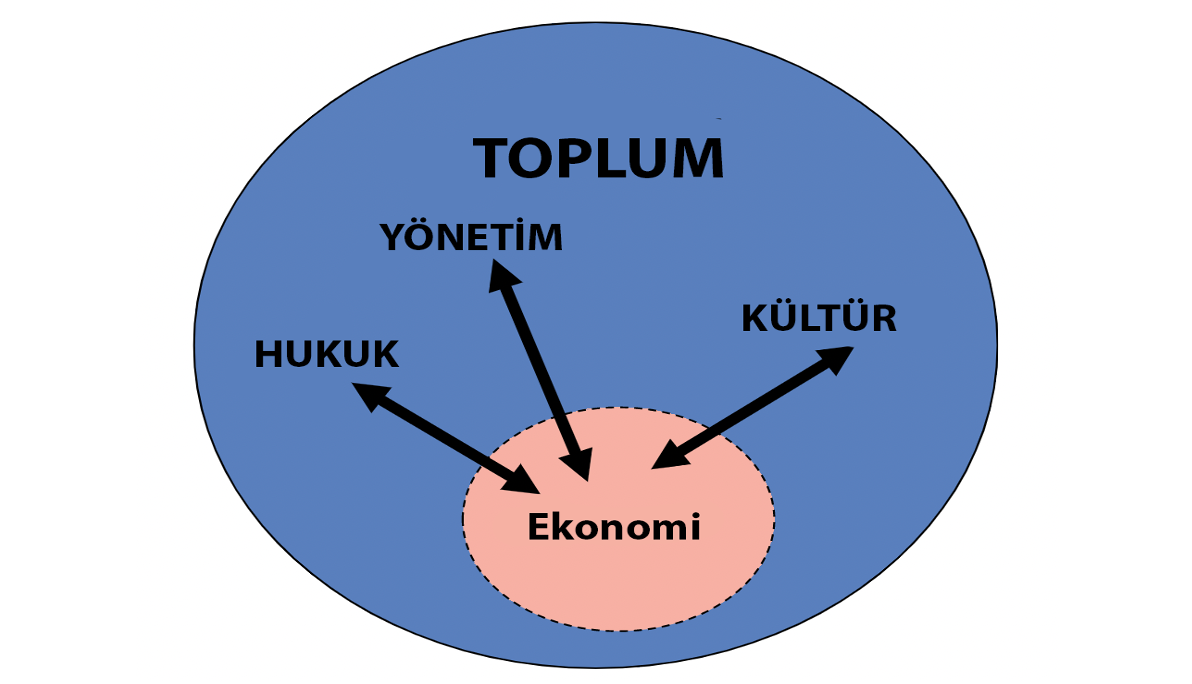
\includegraphics[width=0.95\linewidth,height=0.95\textheight]{tablolar-sekiller/sekil-2-4} \caption{Kaynak: (Harvey, 2016:21)}\label{fig:unnamed-chunk-5}
\end{figure}

Kaynak: (Harvey, 2016:21)

\textbf{Şekil 2.5:} Toplumlar (Ekonomiler) Farklı Kaynak Ortamlarında Nasıl Farklı Yapılandırılmıştır?

\begin{figure}
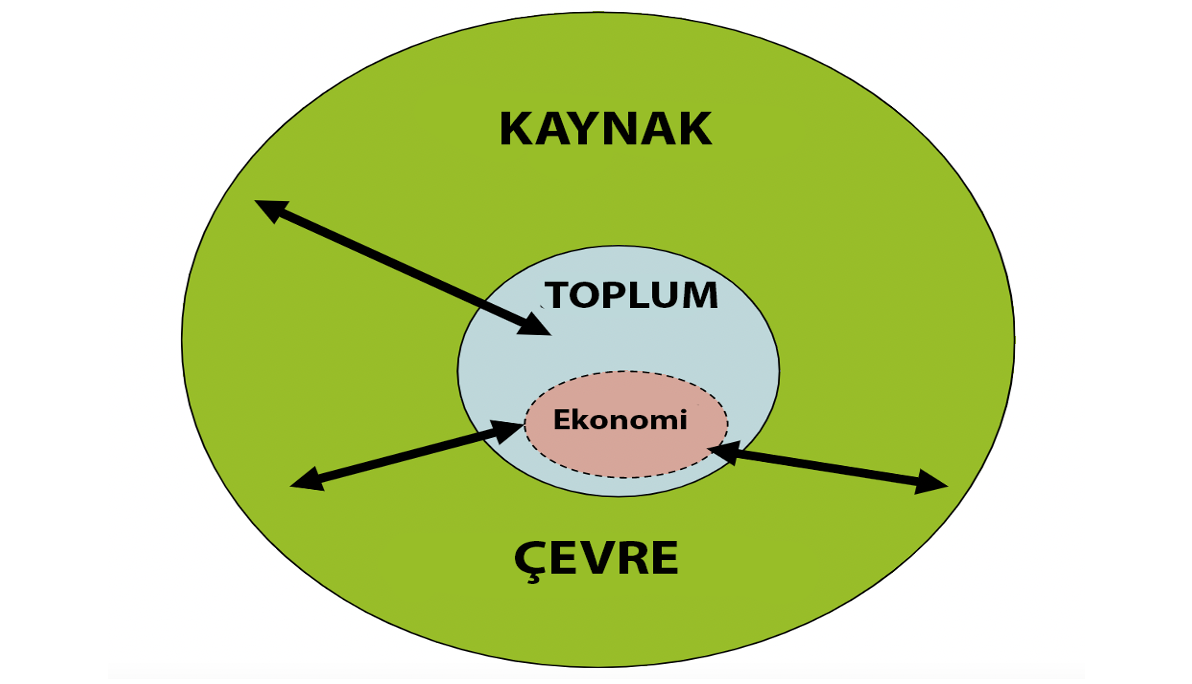
\includegraphics[width=0.95\linewidth,height=0.95\textheight]{tablolar-sekiller/sekil-2-5} \caption{Kaynak: (Harvey, 2016:21)}\label{fig:unnamed-chunk-6}
\end{figure}

Kaynak: (Harvey, 2016:21)

Dolayısıyla, sosyogenez bir perspektiften, servet (kişi başına gayri safi yurtiçi hasıla açısından) ve iklim değişikliği üretimi (yılda kişi başına düşen CO2 emisyonu) arasındaki ilişkidir. İkisi arasında doğrudan bir ilişki vardır, bir ulusun kişi başına ortalama serveti ne kadar yüksekse kişi başına düşen sera gazı emisyonu o kadar büyük olmaktadır. Ripple ve arkadaşları (2019) ülkeleri atmosfer üzerindeki ulusal toplam sera gazı GHG etkisinden ziyade üretimi açısından yeniden sıralamaktadır. Yoğun bir şekilde kentleşmiş ve enerji ithalatına bağımlı Singapur hariç, ABD masanın başındadır ve Çin on ikinci sıraya düşmektedir. Bir ABD vatandaşının ortalama servet üretimi, bir Çin vatandaşının ortalama servet üretiminden altı kat daha fazladır ve ortalama bir vatandaş, bir Çin vatandaşından iki buçuk kat daha fazla CO2 eşdeğeri üretmektedir. Hindistan örneği daha da çarpıcıdır. Ortalama bir ABD vatandaşı, ortalama bir Hintliden 30 kat daha fazla servet ve dokuz kat daha fazla CO2 üretmektedir. Aşağıda daha ayrıntılı olarak incelenecek olan Avrupa Birliği, Amerika Birleşik Devletleri vatandaşı başına servetin yarısından biraz fazlasına ve kişi başına düşen CO2'nin yarısından daha azına sahiptir (Harvey, 2016: 163). Eden, iklim krizini, birçok meselede olduğu gibi bunu da bir adalet sorunu olarak görür. Siyasal elitlerin, zenginlerin dünyada birçok meseleden muaf olduğu gibi bu krizden de muaf olduklarını ifade etmektedir (s. 31). \citep{eden2015iklim}

Hem kişi başına zenginlik hem de kişi başına düşen CO2 grafiğinin aşağı doğru eğrisine bakıldığında birkaç ani düşüş görülmektedir. Bunlar, politik ekonomilerin yukarıda bahsedilen kaynak ortamları ana fikrini desteklemektedir: Bu ani işaretler, zenginliği önemli ölçüde petrol veya kömürden (Birleşik Arap Emirlikleri, Suudi Arabistan, Kazakistan, İran) elde edilen ülkeleri temsil etmektedir. Brezilya örneğindeki düşüş, elektrifikasyon veya ulaşım için enerjisinin çok azını fosil yakıtlardan almaktadır. Suudi Arabistan, Brezilya'dan üç kat daha fazla kişi başına CO2 üretmektedir. Kömür kaynaklarıyla Avustralya da yüksek düzeyde CO2 ortaya çıkarmaktadır (s. 163). \citep{harvey2016climate}

\textbf{Şekil 2.6:} Ulusal Zenginlik ve İklim Değişikliği.

\begin{figure}
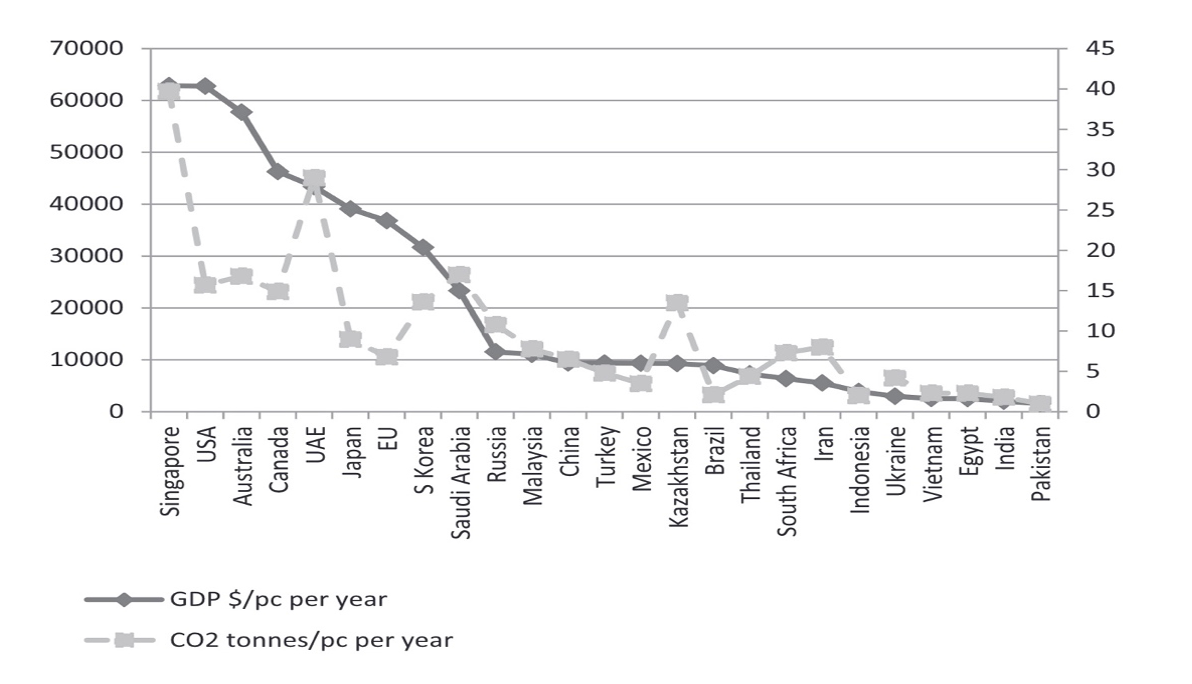
\includegraphics[width=0.95\linewidth,height=0.95\textheight]{tablolar-sekiller/sekil-2-6} \caption{Kaynak: (Harvey, 2016: 162) Kişi başına düşen GSYİH'ye göre sıralanan ilk 25 ülke, en yüksekten (solda) en düşüğe (sağda) yıllık olarak}\label{fig:unnamed-chunk-7}
\end{figure}

Kaynak: (Harvey, 2016: 162) Kişi başına düşen GSYİH'ye göre sıralanan ilk 25 ülke, en yüksekten (solda) en düşüğe (sağda) yıllık olarak

\citet{eden2015iklim}'e göre; iklim siyasetinin ön plana çıkmamasının nedeni, toplumsal konjonktürden kaynaklı stratejik bir tercih olabilir. Türkiye gibi politik gündemin çok hızlı değiştiği ülkelerde iklim siyasetinin yer bulamayışının sebeplerinden bir tanesidir (Eden, 2015: 33).

Chomsky'nin belirttiği gibi, iklim kriziyle ilgili yapmamız gereken yeni görevler bulunmaktadır ve bunun acil bir durum çağrısı olduğu kabul edilmelidir. Tarih, korkunç savaşlar, tarifsiz işkenceler, katliamlar ve akla gelebilecek her türlü temel hak ihlali kayıtları bakımından oldukça zengindir. Örgütlü insan yaşamının ortadan kalkma tehdidi tümüyle yenidir. Bunun üstesinden tüm dünyanın ortak çabalarıyla gelinebilir. Sorumluluk kapasiteyle doğru orantılıdır. Temel ahlaki ilkeler, dünyamız için korkunç bir gelecek yaratırken, kendilerini zenginleştiren ve yüzyıllardır krizler yaratanlara özel bir yükümlülük getirmektedir (s. 20). \citep{chomsky2020} Avusturyalı iklim bilimci Andrew Glikson'a göre; dünya ordularına senede yaklaşık 1,8 trilyon dolar harcanmaya devam ediliyor ve bu kaynak, dünyadaki yaşamın korunmasına yönlendirilmelidir (s. 24-25). \citep{chomsky2020}

\hypertarget{iklim-deux11fiux15fikliux11fi-iletiux15fimi-ve-aktuxf6rleri}{%
\chapter{İKLİM DEĞİŞİKLİĞİ İLETİŞİMİ ve AKTÖRLERİ}\label{iklim-deux11fiux15fikliux11fi-iletiux15fimi-ve-aktuxf6rleri}}

İnsan topluluğu, hayatta kalmak için doğaya bağlıdır. Son derece gelişmiş ve uzmanlaşmış insan toplumumuz içinde yaptığımız her şey, yaşayan ve sağlıklı bir gezegende sağlanan hizmetlere bağlıdır. Dünya, insanlığın sahip olduğu tek gezegen ve evdir. Biyosferin işlevleri insanlığı ayakta tutmaktadır. Doğal sistemler, bize temiz hava, temiz su, barınak, zevk, güzellik ve insanlığı aşan işlere olan inancımızı vermektedir. Dünyadaki en önemli tesis olarak kurulan ekonomimiz de doğanın ekonomisine bağlıdır. Özet olarak, doğa yaşar ve çalışırsa, biz de yaşayabilir ve çalışabiliriz. Gezegenimizin bizlere vermiş olduğu açık mesajlar bulunmaktadır. Bu mesajları anlamaya çalışmak, bilimin çalışmasını kavramsallaştırmanın bir yoludur. Bilim insanları ve tüm çevresel iletişimciler için bu mesajlar çok önemli bir bilgi kaynağıdır. Çevresel iletişimcilerin, bilim insanları ve teknik olmayan, daha geniş kitleler arasındaki ara konumu çok önem arz etmektedir. Çevresel iletişimciler, dünyamızın onlar aracılığıyla ne söyleyeceğini anlamak ve bunu aktarmak için kendi algısal becerilerini geliştirmeleri gerekmektedir (s. 4). \citep{jurin2010environmental}

Dünyanın dört bir yanından araştırmacılar, iklim değişikliğini daha iyi anlamak için çalışırken başka bir akademisyen kadrosu da iklim değişikliğinin en iyi nasıl anlatılabileceği ve iletilebileceği üzerine çalışmaktadır. İletişim araştırmacıları olarak, bu iletişim faaliyetlerinin gerçekleştirilmesi için yeni bir paradigmanın düzenlenmesi gerekmektedir (s. 31). \citep{hansen2016communicating} Bilim, ikna edici iletişimciler olarak yeterli olmayabilir. Toplumlarda, bilim insanlarına olan güven yüksek olsa da iklim değişikliğiyle ilgili somut gerçeklerin yeterli olmadığı gibi bu da yeterli olmayabilir. Bilim insanlarının seslerinin, iklim konusunda açıkça duyurulması gerekmektedir (s. 37). \citep{hansen2016communicating} İklim krizini topluma anlatmak için iklim aktörlerinin faaliyetlerine ihtiyaç vardır. Bölümün ilerleyen kısmında bu aktörlere değinilecektir. Bu uygulamaların gerçekleşmesi için çevre iletişimi ve iklim değişikliği iletişimi kavramları önem arz etmektedir. Çevre iletişimi ve iklim değişikliği iletişimi, birbirinden bağımsız kavramlar olmadığı için çalışma içerisinde, her iki kavram da değerlendirilmiştir. Literatürde, iklim değişikliği iletişimi, çevre iletişimi içerisinde de değerlendirilmektedir.

\hypertarget{uxe7evre-iletiux15fimi}{%
\section{Çevre İletişimi}\label{uxe7evre-iletiux15fimi}}

Çevre iletişimi tüm iletişim uygulamalarını kapsayan çevresel konu ve problemler hakkındaki sosyal tartışmaların kesişme noktası olarak tanımlanmaktadır. Çevre iletişimi, kişiler arası iletişimden, sanat topluluklarından sivil toplum gibi katılımcı gruplara kadar olası tüm etkileşimleri içermektedir. Alexander Flor iletişim yaklaşımlarını; prensiplerinin, stratejilerinin ve tekniklerinin çevre yönetimi ve korunması üzerine yapılan çalışmalar olarak tanımlamıştır (s. 4). \citep{flor2004environmental}

Çevre bilimi disiplinler arasıdır. Flor; kimyagerlerin, biyologların, jeologların ve mühendislerin daha sonradan çevre bilimine dâhil olduklarını, bunların çevre bilimci olarak eğitilmediğini ve daha sonradan çevre bilimine eklendiğini belirtmektedir. Çevre biliminin disiplinler ötesi olduğunu ve bu konuda büyüyen bir alan olduğunu vurgulamaktadır. Çevre biliminin, her zamankinden daha fazla eleştirel olarak, sosyal analiz ve sosyal eylem gerektirdiğini vurgulamaktadır. Sonuç olarak, çevre uzmanlık saflarının giderek arttığını ifade etmektedir. Bu meslek grupları; kimyagerler, biyologlar, jeologlar, mühendisler, antropologlar, sosyologlar, ekonomistler, avukatlar, siyaset bilimciler ve iletişim bilimciler gibi çalışma alanlarını kapsayan şekilde genişlemektedir. \citep{flor2004environmental} Bu araştırmada, iklim değişikliği iletişimi kapsamında, iklim aktörlerinin daha iyi bir iletişim stratejisi kurmalarına yönelik önerilerde bulunulmaktadır. İklim krizine dikkat çekmeyi ve iklim aktörlerinin iletişim faaliyetlerinin halkla ilişkiler kapsamında bir analizini ortaya koymayı amaçlamaktadır. Yapılan araştırma sonucunda çıkan sonuçlar yukarıda bahsedilen meslek alanlarına da uygulanabilir şekilde geniş bir perspektif sunmaktadır.

Coğrafi sınırları aşan, insanlar ile doğa arasındaki simbiyotik ilişkileri keşfeden sürdürülebilirlik, çevresel yönetişimde katılımcı karar verme ve iş birliği gibi bu tür katılımcı yaklaşımlar, kamu bilincini, bilinçli kişisel seçimleri, çevrenin korunmasını ve kurumsal sektör tarafından çevresel faaliyetlerin iyileştirilmesine katkıda bulunmaktadır (s. 7). \citep{fyfe2010advanced}

Çevrecilik, çevresel iletişimle başlamıştır. Bir biyolog olan Rachel Carson, 1962 yılında daktilosundan çıkan Silent Spring kitabının yayınlanmasıyla çevresel iletişimin ilk örneklerinden biri olarak gösterilmektedir (s. 3). \citep{flor2005environmental} İnsanlar birbirleriyle ve doğayla etkileşime girdiğinden beri çevresel iletişim var olmuştur. Ancak, uygulayıcılar ve akademisyenler tarafından geniş bir mutabakatla uygulanan bir adlandırma olarak ``çevresel iletişim'' 1969 yılına dayanan çok daha kısa bir tarihe sahiptir. Journal of Environmental Education, 40 yıl önce yayımlandığında, çevre eğitimi ve iletişimi aynı görülmekteydi. \citet{schoenfeld1969whats} derginin ilk sayısında yer alan ``What's New about Environmental Education?'' adlı makalede çevre eğitimini; çevre sorunları hakkında bilgi sahibi, bu sorunların çözümünde yer alacak bir vatandaş yetiştirmeyi amaçlayan iletişim olarak tanımlamıştır. Sonraki yıllarda da bu sorunları çözme ve farkındalık oluşturma motivasyonlarını oluşturmaya yönelik çalışmalarda çevre eğitimi ya da iletişimi olarak adlandırılmıştır (s. 5). \citep{jurin2010environmental}

Çevre iletişiminin periyodik geçmişi açıklandığında, 1960'ların sonlarında ortaya çıkan gençlik hareketleri sosyo-politik statükoya karşı başlatılmış protestolardır. Bu protestolar, savaş karşıtı mesajlarla birlikte, çevre kirliliğine karşı taleplerle ve endüstrilerin faaliyet gösterdiği ulusal alanlarda ve çevre yönetiminde iyileştirmelere yol açmıştır. Çevresel süreli yayınların ilk dalgası olan 1969'daki 31 yayın, 1974 yılına gelindiğinde 209'a yükselmiştir (s. 12). \citep{jurin2010environmental}

Yıldönümleri, kitle hareketleri için motive edici olabilmektedir. Dünya Günü'nün 20. yıl dönümü, Amerika Birleşik Devletleri'nde çevreciliğin tekrar canlanmasını sağlamıştır. 1992'deki Rio Zirvesi'nde, insan nüfusu ve sosyal adalet konuları ön plana çıktı ve bu nedenle çevresel bozulmalar, bu bozulmaların semptomlarına, nedenlerine ve çözümlerine odaklandı. Çevre yayınları 1980'lerde bir plato grafiği göstermektedir. Zirvenin etkisiyle, 1993 yılında çevre yayınları sayısı ilk kez 500'ün üzerine çıkmıştır. Çevre iletişimi 2002 yılında üçüncü dalgasını yaşamıştır. Bu dalgada, çevresel yayın sayısı artmış ve her zamankinden daha fazla yayında çevresel içerik yer almaya başlamıştır. Çevre indeksi veri tabanında, 1187 süreli yayın kataloglanmıştır (s. 13). \citep{jurin2010environmental}

Cox ve Pezzullo, çevre iletişimini informal ve formal olarak iki şekilde tanımlamaktadır: \citep{cox2018}

\textbf{İnformal:} Çevre iletişimi, su kirliliği, boz ayı habitatı gibi çevresel konular hakkında konuşma ve bilgi aktarımı olarak tanımlanır. Bu iletişim, çevre hakkında nasıl iletişim kurduğumuzu ve bu iletişimin hem çevre üzerindeki etkilerini hem de kendi algılarımız üzerindeki etkilerini kapsar, böylece doğal dünya ile ilişkilerimizi de içine alır.

\textbf{Formal:} Çevre iletişimi hem çevreyi hem de doğal dünyayla olan ilişkilerimizi anlamamızı hem pratik hem de kurucu araç olarak kullanılmasıdır. Çevre sorunlarını ifade ederken ve toplumun farkındalığını müzakere ederken kullandığımız sembolik bir araçtır. Pragmatik kısım; eğitme, uyarma, ikna etme ve çevre sorunlarını çözme alanlarını kapsamaktadır. Kurucu kısım ise; dil ve diğer sembiyotik eylem biçimlerini temsil eden daha ince bir düzeydir. Anlayış ve algısal olarak doğa ve çevre sorunlarının temsillerini inşa etmemizi ya da oluşturmamızı temsil etmektedir.
Corbet, ``Communicating Nature: How We Create and An Environmental Messages'' adlı kitabında genişletilmiş bir kapsamda aşağıdaki maddeler bağlamında çevre iletişimini tanımlanmaktadır (s.8). \citep{corbett2006} Çevre iletişimi; değerler, kelimeler, eylemler ve günlük uygulamalarla ifade edilmektedir.

• Bireysel olarak yorumlanır ve müzakere edilir.
• Tarihsel ve kültürel olarak kök salmıştır.
• İdeolojik olarak türetilir ve yönlendirilir.
• Çevresel iletişim, çevreye araçsal değer atfeden ve onun insanlara hizmet etmek için var olduğuna inanan baskın bir sosyal paradigmanın içine yerleştirilmiştir.
• Karmaşık bir şekilde popüler kültüre, özellikle reklam ve eğlenceye bağlıdır.
• Medya tarafından genel olarak statükoyu destekleyecek şekilde çerçevelenir ve raporlanır.
• Hükümet ve iş dünyası gibi sosyal kurumlar tarafından yönlendirilir ve etkilenir.

Çevre iletişimi, gezegenin bozulmasına yönelik insanları ikna etmenin yollarını aramakla görevli bir kriz disiplinidir. İnsanların hem doğal biyolojik sistemlerin hem de insan topluluklarının refahıyla ilgili çevresel sinyallere uygun şekilde yanıt verme yeteneğini geliştirmek olarak alanın amacı tanımlanmaktadır. Şu an dünya bir krizin içerisindedir. Krizi iyi yönetmek adına çözüme odaklı bir yol haritasıyla halkla ilişkiler uygulayıcıları iletişim planlarını oluşturmalıdırlar. Burada kurumsal sosyal sorumluluk bağlamında şirketlerin yaptığı iletişim faaliyetlerinden sivil toplum kuruluşlarının yaptığı tüm iletişim faaliyetleri için geçerlidir. Bu krizin çok boyutlu ve karmaşık yapısı gereği her bir aktöre önemli sorumluluklar düşmektedir.

\hypertarget{uxe7evre-iletiux15fimi-modelleri}{%
\section{Çevre İletişimi Modelleri}\label{uxe7evre-iletiux15fimi-modelleri}}

Jurin ve arkadaşları, çevre iletişimi için iki model önermektedir. Bunlardan ilki 1973 Witt'in modelinden genişletilmiş ve uyarlanmış olan ``Çevresel İletişim Bilgi Modeli'', ikincisi ise, Foulger'in modelinden uyarlanan ``İletişim Sürecinin Ekolojik Modelidir'' (s. 15). \citep{jurin2010environmental}

\hypertarget{uxe7evresel-iletiux15fim-bilgi-modeli}{%
\subsection{Çevresel İletişim Bilgi Modeli}\label{uxe7evresel-iletiux15fim-bilgi-modeli}}

Bu model, farklı aktörlerden gelen çok sayıda çapraz bilgi akışının yanı sıra, onaylanmış mesaj türlerinin daha geniş bir kitleye nasıl yerleştirildiğini göstermeye yardımcı olmaktadır. Oklar, hattın ağırlığına uyan olağan akış gücü ile ana bilgi akışlarını temsil etmektedir. Model, çevreyi mesajın aktığı ortam olarak göstermektedir. Bu model içerisinde yer alan kurum ve kuruluşlar, ileri de anlatacağımız iklim aktörlerini de temsil etmektedir.

\textbf{Şekil 3.1:} Çevresel İletişim Bilgi Modeli.

\begin{figure}
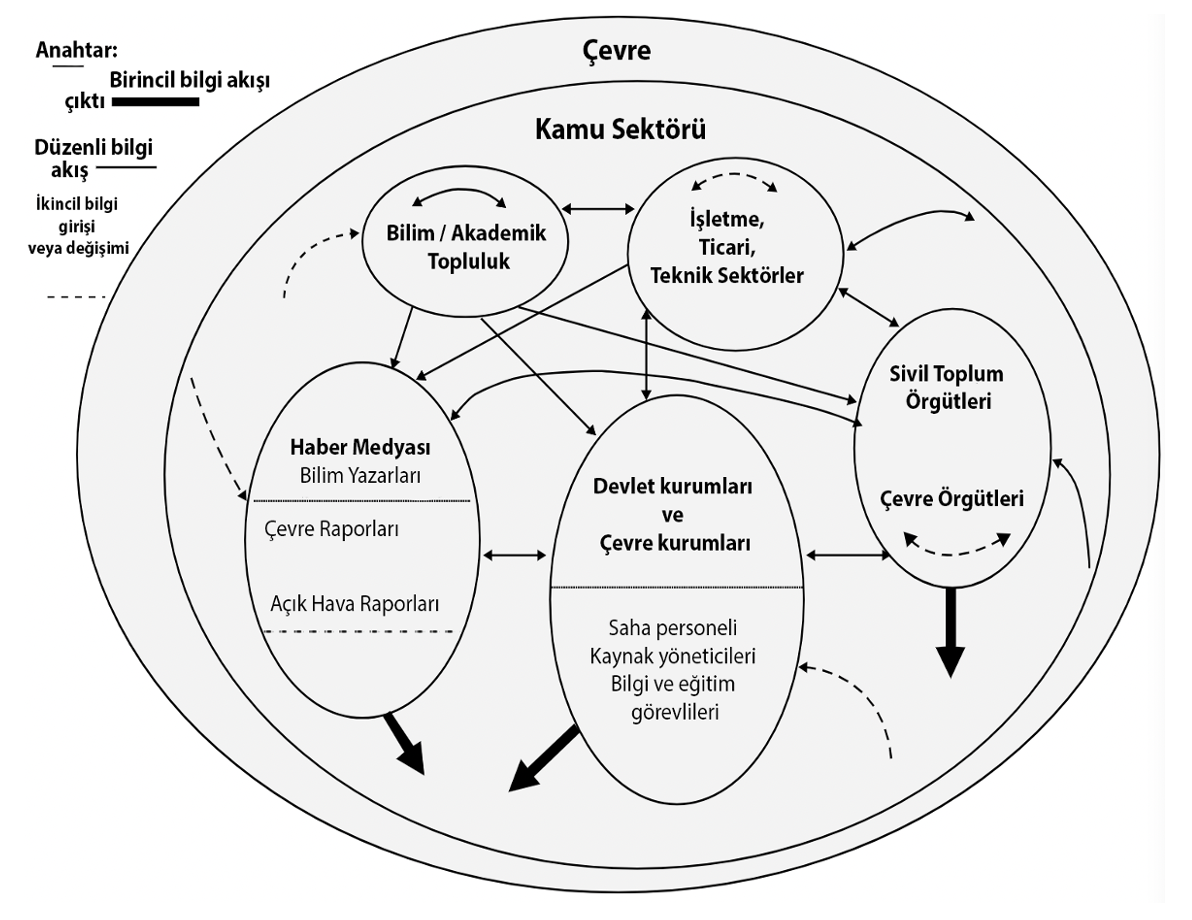
\includegraphics[width=0.95\linewidth,height=0.95\textheight]{tablolar-sekiller/sekil-3-1} \caption{Kaynak: (Harvey, 2016:21)}\label{fig:unnamed-chunk-1}
\end{figure}

``Çevresel İletişim Bilgi Modeli'' internetin ortaya çıkmasından çok önce tasarlanmıştır. İnsan grupları, tekil ortamımızda halen mesajların kaynağı ve alıcısı konumundadırlar. İnternet, mesajların hacmini ve hızını önemli ölçüde arttırmış olabilir ancak bu, daha büyük, hızlı ve geniş bilgi hattı, insanların mesaj oluşturmasına ve tüketmesine ihtiyaç duymaktadır (Jurin ve diğerleri, 2010: 16).

Bu model de gerekçeleri bilimsel bilgilere dayandığı için akademik topluluklar en güvenilir kaynak olarak görülme eğilimindedir. Ancak bu dergilerin okuyucuları genelde akademik çevreler olduğu için bilgiler sınırlı sayıda kişiye ulaşmaktadır. İşletmeler ise, iletişimlerini pazarlama ve reklam aracılığıyla gerçekleştirmektedir. Bu mesajların çoğu ürün ve hizmetlerini satmak için yapılır. Yasal yükümlülüklerini yerine getirmek için devlet kurumlarıyla da iletişim kurarlar. Haber medyası, birincil önceliği güncel olayların raporlanması ve analizidir. Hedef kitlesi kamu kitlesidir. Devlet kurumları; hükümetler ve özel kuruluşlar arasında kanunları, kuralları ve düzenlemeleri aracılığıyla yaptırım ve uyum eylemlerini gerçekleştirirler. Kamu sektörü, aynı zamanda, kitle iletişim araçları ve ayrıca hükümet park birimleri ve kamu arazileri aracılığıyla, sosyal yardım ve eğitim çabalarının birincil hedef kitlesidir. Kamu sektörü; ajansları ve yetkilileri ilgili konularda uyararak daha küçük bir geri bildirim rolüne sahiptir. Sivil Toplum Kuruluşları (STK); çevresel bilgileri kullanarak kendilerine ait ikna edici bir iletişim ağını sürdürürler. Birincil izleyiciler, üye iletişimleri, kitle iletişim araçları ve hükümet temsilcileri üzerindeki baskı yoluyla kamu sektörüdür. İkincil izleyiciler, kurumsal çıkarları söz konusu olduğunda finansman ve politika değişikliği desteği sağlayabilecek iş sektörü ortakları olacaktır. Bu iletişimsel ilişkiler, STK iş sektörünün iş yapış davranışını değiştirmeye çalıştığında gerginlikler ortaya çıkabilmektedir (s. 17-18). \citep{jurin2010environmental}

\hypertarget{iletiux15fim-suxfcrecinin-ekolojik-modeli}{%
\subsection{İletişim Sürecinin Ekolojik Modeli}\label{iletiux15fim-suxfcrecinin-ekolojik-modeli}}

Foulger'a göre, iletişim; mesaj oluşturucuları, mesajı alanları ve mesajın kendisini içermektedir. Mesajları zihinler arasında taşımak için dil ve medya gerekmektedir. Mesaj oluşturucular ve alıcılar arasındaki ilişkiler anlamların şekillendiğinden, değiş tokuş edildiğinden ve bunlara tepki verildiğinden dinamik, döngüsel ve çok yönlüdür. Mesajların oluşturulması ve tüketilmesi, bireyler içerisinde genellikle aynı anda gerçekleşmektedir (s. 18). \citep{jurin2010environmental}

\textbf{Şekil 3.2:} İletişim Sürecinin Ekolojik Modeli.

\begin{figure}
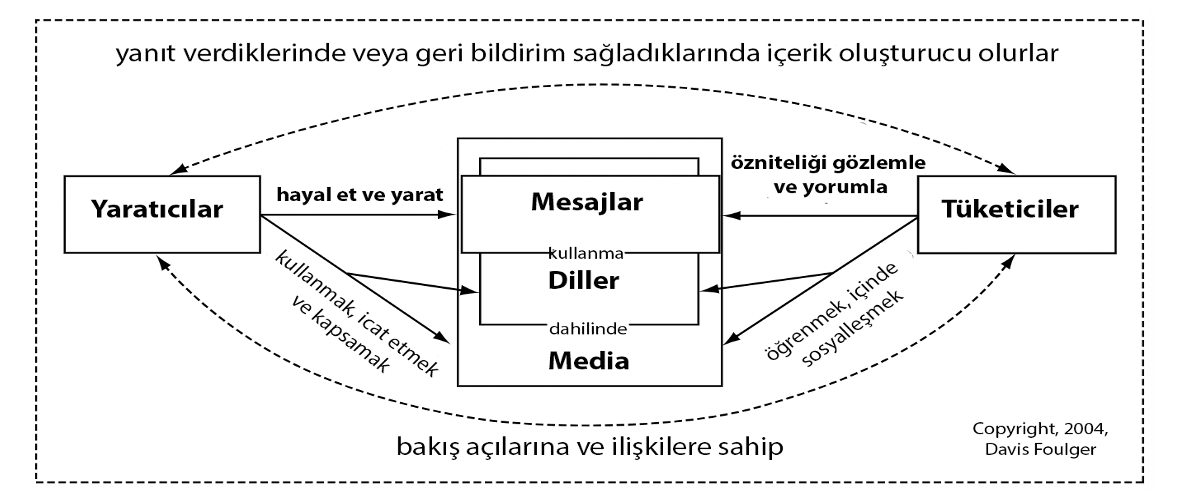
\includegraphics[width=0.95\linewidth,height=0.95\textheight]{tablolar-sekiller/sekil-3-2} \caption{Kaynak: (Mavimbela ve diğerleri, 2018: 42)}\label{fig:unnamed-chunk-2}
\end{figure}

Anlam, kişinin zihninde başlar. Bu eylem, dil ve aracı kullanana kadar soyuttur. Mesaj oluşturucu olarak kişi, somutlaştırılmış fikirlere sahiptir. Foulger, dillerin ve medyanın zaman içerisinde geliştiğini ve dolayısıyla iletişimin yaratılmasının bir parçası olduğunu belirtmektedir. Dil ve medyayı kullanmak beceri gerektirmektedir. İnsanların mesaj oluşturabilmeleri ve yorumlamaları için dil ve medya öğrenmeleri gerekmektedir (s. 19). \citep{jurin2010environmental}

``Çevre İletişim Bilgi Modeli'' gruplar arası iletişimle ilgilenirken ``İletişim Sürecinin Ekolojik Modeli'' ise kişiler arası iletişime odaklanmaktadır. İlk model, büyük olayları anlamak için daha uygundur; ikinci model ise daha mikro iletişime indirgeyerek bireysel seviyede ele almaktadır. Tarihsel olarak, bu süreç iletişimi kitle iletişimi ve kişiler arası iletişim olarak ele alınmıştır. Ancak iletişim çevrimiçi hale geldikçe bu ayrım ve kavramlar bulanıklaşmıştır. Bununla birlikte, tüm iletişimi yaşadığımız yerden kaynaklanan insani bir süreç olarak tanımlanmaktadır. İletişimin yeri çevremizdir (s. 19). {[}@\citep{jurin2010environmental}{]} Bu açıklama, araştırmanın genel yapısı içerisinde, ``Çevre İletişim Bilgi Modeli'' daha uygun bir model olduğu yorumlanabilir. Ancak, iklim aktörlerinin her birinin iletişim uygulamaları incelendiğinde tek tek değerlendirildiğinde ``İletişim Sürecinin Ekolojik Modeli''nin durumu daha iyi anlatabileceği düşünülmektedir.

Çevre iletişimi 1980'lerden bu yana profesyonel bir alan olarak sürekli gelişmektedir. İletişim, medya, gazetecilik ve enformasyon gibi disiplinlerle sürekli çalışma alanı genişlemektedir. Pezzullo (2017) çevre iletişiminin çalışma alanıyla ilgili yedi genel yaklaşım belirlemiştir (s. 36). \citep{cox2018}

\begin{enumerate}
\def\labelenumi{\arabic{enumi}.}
\item
  \textbf{Çevresel kişisel kimlik ve kişiler arası ilişkiler:} Bireylerin kendi kişisel çevresel tutumlarını ve kişilerarası ilişkilerine odaklanan çevresel iletişim araştırmalarını kapsamaktadır. Tüketim alışkanlıkları, yerinde olma duygusu, çevre eğitimi uygulamaları ya da grupların çevresel tutum ve davranışlarını ele almaktadır. Bu yaklaşım söylemlere, insan olmayan diğer canlılarla ilişki kurma yollarına dair değişen bakış açıları gibi kültürler arası farklılıklara ve diyaloglara da odaklanabilir.
\item
  \textbf{Çevresel organizasyonel iletişim çalışmaları:} Belirli kurumların ya da ağların çevresel konuları nasıl tartıştığını ve örgütlendiğini araştırmaktadır. Bu çalışma alanı hem kamuoyunu hem de günlük yaşamlarımızı etkileyen çevresel ve çevre karşıtı söylemlerin hiyerarşik dilini, hikayelerini, ritüellerini, rollerini, kurallarını araştırmaktadır.
\item
  \textbf{Çevre bilimi, teknolojisi ve sağlık iletişimi:} Laboratuvarlarda ve hastane odalarında kişisel teknoloji tercihleri, kişilerarası, çevre politika belirleyicilerinin risk değerlendirmelerine kadar birçok farklı konuyu değerlendirmektedir. Bu çalışmalar kamusal ya da popüler söylemlerden daha çok hasta-doktor ilişkisi, halk sağlığı kampanyaları, bilim insanlarının halkla daha etkili bir biçimde nasıl iletişim kuracağı üzerine odaklanmaktadır.
\item
  \textbf{Çevresel karar alma süreçlerine toplumsal katılım:} Retorik, söylem çalışmaları, örgütsel iletişimden faydalanmaktadır. Demokratik uygulamaları, kamu malları ve müşterekleri üzerine olan tartışmaları ifade etmektedir. Toplumsal katılımın ve STK, dernek gibi paydaşların çevre politikaları ve projeleri üzerindeki kararlarda etkisi olup olmadığını, katkısının ne ölçüde olduğu gibi konuları araştırmaktadır.
\item
  \textbf{Çevresel kitle iletişim çalışmaları:} İklim üzerine çalışan bilim insanlarının daha fazla kişiye ulaşmaları sonucu ortaya çıkmıştır. Daha çok sosyal bilimsel bir bakış açısına dayanan bu yaklaşım, çevresel konuların ana akım haber kapsamına ilişkin söylem analizlerini, medyada çevrenin sosyal inşası ve/veya çerçevelenmesi çalışmalarını, görsel yeşil markaları, yeşil pazarlama ve çevresel medya etkilerini içermektedir.
\item
  \textbf{Yeşil uygulamalı medya ve sanat:} Fotoğraf, video, ses, canlı performans gibi teknoloji tabanlı sanatları kapsamaktadır. Üretmeye odaklanan çevre odaklı çalışan uygulayıcılar ve akademisyenler için geniş çatı bir kavram olarak karşımıza çıkmaktadır. Bu alan çevre gazeteciliği, halkla ilişkiler, yeşil tasarım, çevre mimarisi gibi alanlara da odaklanabilmektedir.
\item
  \textbf{Çevresel retorik ve kültürel çalışmalar:} Kurgu ve kurgusal olmayan arasında köprü kurar. Bireysel ve toplu ifade; sözlü ve sözsüz etkileşimler, yüz yüze veya çevrimiçi iletişim; anlam, önemlilik, etki kaygıları ve daha fazlasını kapsamaktadır. Retorik ve kültürel çalışmalar dil, söylem, görsel metinler, popüler kültür, yer, çevre savunuculuğu kampanyaları, çevre hareketleri, canlı performanslar ve/veya kamusal alandaki tartışmalar gibi bir dizi iletişimsel olgunun analizini içermektedir. Bu tür çalışmalar için bağlam, ses, yaratıcılık ve yargı hakkında düşünmek hayati önem taşımaktadır. Retorik ve kültürel çalışmalar belirli durumlar veya konjonktürler içindeki kurumlar ve iktidar arasındaki ilişkiyi araştırmaktadır. Konular, çevresel adalet hareketinden ırksal adaletsizliklere ve çevresel bozulma arasındaki ilişkiyi ön plana çıkarması da dahil olmak üzere çok çeşitlidir. İnsan ve hayvan ilişkilerinin metalaştırılması ve çevresel belgesel filmlerin veya bilim kurgu filmlerin kültürel önemi gibi farklı konuları işleyebilir.
\end{enumerate}

Çevreyi ilgilendiren uygulamalar noktasında; devletler, yerel yönetimler ve özel sektörün ağırlığı dünyada daha fazla görülmektedir. Bu uygulamalar genelde vatandaşların aleyhine olmaktadır. Çevreyi doğrudan ilgilendiren konularda, vatandaşların talepleri çoğu zaman göz ardı edilmektedir. Vatandaşların ormanların korunması, çevre kirliliği, hayvanların yaşam koşulları gibi konularda söz sahibi olması için sivil toplum kuruluşları, dernekler, vakıflar aracılığıyla seslerini duyurmaları, hak taleplerini iletmeleri daha kolay olmaktadır.

\hypertarget{iklim-deux11fiux15fikliux11fi-iletiux15fimi}{%
\section{İklim Değişikliği İletişimi}\label{iklim-deux11fiux15fikliux11fi-iletiux15fimi}}

İklim değişikliği iletişimi, çeşitli paradigmalardan teoriye uyarlanmıştır. Risk iletişimi, kalkınma haberciliği, çevre iletişimi, savunucu gazetecilik ve toplumsal değişim ve gelişim için iletişim gibi yaklaşımlar benimsenir (s. 109). \citep{evans2018communicating}

İklim değişikliğinin ne olduğunun hem uluslar hem de bireyler için ne anlama geldiğinin daha iyi anlaşılmasının gerekli olduğu genel olarak bilinmektedir. Daha iyi iletişim kurmaya yardımcı olabilecek yaklaşımların, süreçlerin, yöntemlerin ve araçların belirlenmesi ihtiyacı vardır. Ayrıca, bu fenomeni ve bunun birçok sonucunu ele almak için ihtiyaç duyulan sektörler arası eylem türünü harekete geçirmek için toplum ve paydaşlar arasında iklim değişikliğiyle ilgili konularda iletişimin nasıl gerçekleşebileceğine dair başarılı örnekler sergilenmesi ihtiyacı vardır.

Kriz anlarıyla ilgili en önemli etmen, en etkili ve kolay çözüm için doğru yerde olmaktır. İklim ve diğer afetler noktasında kırılganlığı en aza indirgemek için topluluk gelişiminin planlanması gerekmektedir. Bunun yapılması için; planlamacılar, iklim değişikliği uzmanları, risk iletişimi profesyonelleri arasında sürekli diyalog gerektiren bir sistemin gerekliliğini ortaya koymaktadır. Tehlikeli kriz anlarında öncesinde, aktörler arasında bilgi alışverişi yapılması kriz yönetiminin ve iletişiminin merkezinde yer almaktadır. \citep{drake2016communicating}

Günümüzde, dünya çapında daha sık ve yoğun doğal afetler üreten aşırı hava koşulları görülmektedir. İletişim; tahmin, hazırlık, azaltma, önleme, iyileştirme, esneklik uygulamaların yapılaması için her kriz ve her noktada önemli bir rol oynamaktadır. Yirmi birinci yüzyıl; dünya ve sosyal bilimcilerinin, bireylerin ve toplulukların doğal afetlerden hızla kurtulma kapasitesini geliştirmelerine yardımcı olmak için birlikte çalışmalarını gerekli kılmaktadır. Dolayısıyla, çok disiplinli bir bakış açısına ihtiyaç duyulmaktadır (s. 2). \citep{drake2016communicating} Kriz yönetimi, krizlerle mücadele etmek ve etkileri en aza indirmeyi amaçlar. Diğer bir tanımla, bir krizin olumsuz sonuçlarını önlemeyi veya azaltmayı böylece organizasyonu, paydaşları, endüstriyi zararlardan korumayı hedefler. Coombs'un kriz iletişimi, önleme, hazırlık, müdahale ve revizyon olmak üzere dört faktörden oluşur (Coombs, 2014: 21). İletişim, kriz yönetiminin sadece bir parçasıdır. Kriz iletişimi, olumsuz olay öncesinde, sırasında ve sonrasında kuruluş ile kamu arasındaki diyaloğu sağlar. Bu noktada, iklim değişikliği nedeniyle ortaya çıkabilecek olaylar karşısında toplumların bilinçlendirilmesi, bu krizi iyi yönetmek için bilgilendirmelerin, gerekli eğitimlerin verilmesi gerekmektedir.

\hypertarget{iklim-deux11fiux15fikliux11fi-ve-medya}{%
\subsection{İklim Değişikliği ve Medya}\label{iklim-deux11fiux15fikliux11fi-ve-medya}}

İklim değişikliği ve medya konusu sürekli genişleyen, çeşitliliği olan bir akademik alandır. Yapılan bir meta-analiz çalışması, iklim değişikliği ve medya konusunun yıllar içerisinde arttığını göstermektedir. Analitik yelpazenin farklı ülkeler arasında, sosyal medya, çevrimiçi medya dahil olmak üzere daha fazla medya türünü ve farklı metodolojik yaklaşımları içerecek şekilde genişlediğini ortaya koymaktadır. \citep{schaefer2014media}

İklim değişikliğinin medyadaki temsilleri hem sıradan vatandaşlar hem de karar vericiler gibi birçok birey için ana bilgi kaynağıdır. Buna göre, son yıllarda çok sayıda çalışma iklim değişikliğinin medyada nasıl tasvir edildiğini analiz etmiştir. Yapılan bir meta-analiz araştırması, bu alanın gelişimini ve özelliklerini özetlemiştir. Bu meta-analiz çalışması 133 ilgili çalışmayı incelemeye ve ne zaman yayınlandıklarını, hangi ülkeleri ve medyayı analiz ettiklerini ve hangi metodolojik yaklaşımları ve araştırma tasarımlarını kullandıklarını ortaya çıkarmıştır. Bu araştırma sonucunda, iklim değişikliğinin medya temsillerine yönelik araştırma yöneliminde net bir büyümenin olduğu gösterilmiştir. Son yıllarda, özellikle 2000'li yılların ortalarından itibaren giderek daha fazla çalışma yayımlanmıştır. Ayrıca, son yıllardaki medyada yer alan haberler, önceki medya portrelerine kıyasla çok daha fazla bilimsel ilgi görmüştür. Bilimsel ilginin bu açık ve her iki boyutta da büyük ölçüde sürekli büyümesi, iklim değişikliğinin dünya çapında aldığı artan medya ilgisini yansıtmaktadır; \citep{schmidt2013media} konunun vatandaşlar ve karar vericiler için önemli bir sorun haline geldiği gerçeğine tekabül etmektedir (Nisbet ve Myers, 2007). \citep{nisbet2007polls}

Haber medyasının üç etkiye dayandığı belirtilmektedir (Hansen ve Depoe, 2020: 170).
• \textbf{Kamuyu bilgilendirme:} Bilimsel konularla ilgili halkı bilgilendirmek onları teşvik etmek.
• \textbf{Gündem belirleme:} Belirli bir konunun önemine ilişkin kamu algısını etkilemek.
• \textbf{Çerçeveleme:} Halkın bu tür meseleleri nasıl algıladığını çerçevelemek.

İklim değişikliğiyle ilgili toplumsal etki ve tepkilerle ilgilenen bilim insanları, iklim konusunun medyada yer alma düzeyleri ve medya metinlerinin içeriği, halkın ne ve nasıl düşündüğünü araştırmışlardır. Kamu bilgilendirme, gündem belirleme ve çerçeveleme her biri iklim değişikliğinin medyada yer almasına ilişkin farklı araştırma kollarını etkilemiştir. İlk dönem çalışmalar haber medyasının halkı bilgilendirme noktasında normatif rolünü yerine getirip getirmediğine odaklanmıştır.
Gündem belirleme aşaması, bilim insanlarının konunun önem derecesini, medyanın konuyu nasıl desteklediğini veya engelleyebildiğini incelemeye odaklanmaktadır. Schäfer ve Schlichting tarafından yapılan bir meta-analiz çalışması, iklim değişikliği konusunun birçok farklı ülkede ve farklı medya türlerinde nasıl temsil edildiğini incelemiştir. \citep{schaefer2014media}

Yer kürenin ısınması konusunda çalışan insanlar iklim kriziyle mücadele ederken, retorik zorluklarla da karşı karşıyadır. Çerçeveleme, iklim değişikliği ve doğal tehlikelerle ilişkili riskler ve krizler hakkında iletişim kurmanın merkezinde yer almaktadır. Sosyal faydayı etkilemeye niyetli bir aktör için çerçevelemenin nasıl çalıştığını anlamak hayati önem taşımaktadır. İklim krizinin kendisi kadar konunun nasıl sunulduğu ve çerçevelendiği de önemlidir (s. 2). \citep{drake2016communicating} Entman çerçevelemeyi şu şekilde açıklamaktadır (Entman, 1993). \citep{entman1993framing}

``Çerçevelemek, algılanan bir gerçekliğin bazı yönlerini seçmek ve belirli bir problem tanımını, nedensel yorumunu, ahlaki değerlendirmesini ve/veya tedavi önerisini teşvik edecek şekilde iletişim metninde onları belirgin kılmaktır.''

Çerçeveleme tarafsız olmadığı için para, güç, iletişim konusunda bilgi ve medyaya erişim dahil olmak üzere en fazla kaynağa sahip aktörler baskın çerçevele oluşturabilir ve sürdürebilir. Çerçeveleme düşüncede gerçekleşmektedir. Tüm metinler, görseller, kelimeler, paragraflar, kültür bu kapsamdadır. Örneğin; adlandırma olarak ``iklim değişikliği'' yerine daha acil eyleme geçilmesini ifade eden ``iklim krizi'' başlığının kullanılması, çerçeveleme durumunun belirli bir şekilde sunulmasını ya da sunulmamasını sağlayabilir. Çerçeveleme bir sorunu ya da problemi kamuoyunun ilgisinden de uzak tutabilir. Bazı halkla ilişkiler uygulayıcıları tarafından bu kriz iletişiminin içerisinde yer almaktadır. Fakat, etik bir halkla ilişkiler perspektifiyle, eleştirel bir mercek ile yaklaşan uygulayıcılar sorumlu ve duyarlı bir şekilde kamu refahını öncelik edinebilirler (s. 2). \citep{drake2016communicating}\\
Chomsky, zengin hayır sahiplerinden oluşan bir grubun, söylemleri değiştiren düşünce kuruluşları ve ülkelerdeki en büyük lobi grupları aracılığıyla gerçek sorunların üstünün örtülebileceği, işçi haklarının altının oyulması, sendikaların yok edilmesi, halka yardım edebilecek hükümet politikaları engellemesi gibi faaliyetlerde bulunabileceğini belirtmektedir (s. 65). \citep{chomsky2020}

\hypertarget{iklim-deux11fiux15fikliux11fi-ve-sosyal-medya}{%
\subsection{İklim Değişikliği ve Sosyal Medya}\label{iklim-deux11fiux15fikliux11fi-ve-sosyal-medya}}

Genel olarak, iklim değişikliğine ilişkin bireysel algılar, insanların iklim değişikliğini nasıl algıladıkları, olası çözümler ve buna karşı kendi tutum ve davranışlarını etkileyen karmaşık sosyal, ahlaki, psikolojik, kurumsal ve kültürel süreçlere dayanmaktadır. \citep{mahl2020bit} Sosyal medya bu algıların oluşması için geniş bir zemin sunmaktadır. İklim hareketine yönelik farklı sosyal ağ mecraları yer almaktadır. Aynı zamanda, sosyal medyanın kolay kullanımı, hızlı erişilebilir olması, ucuz maliyeti gibi özelliklerinden dolayı hem organizasyonlar olarak hem de bireysel olarak iklim iletişimine yönelik uygulamaları yaygın hale getirmektedir.

Son yıllarda, sosyal medya ve iklim değişikliği üzerine yapılan çalışmalarda artma eğilimi bulunmaktadır. Özellikle, Twitter araştırmacılara sadece iklim konusunda değil, birçok farklı alanda ve konuda çalışma imkânı sunmaktadır. İklim değişikliğinin sosyal medyadaki temsillerine ilişkin araştırmalar üç alana odaklanmaktadır. \citep{pearce2019social} 1) Kamular; iklim değişikliğiyle ilgili durumlarda en etkin hesapların analizi. 2) Temalar; söylemler, hashtagler ve etiketlenmeler (mentions) 3) Profesyonel iletişim; aktivizm ve kampanya analizlerini kapsamaktadır (s. 171). \citep{hansen2020ireland}

İkinci bölümde küresel ısınma başlığında değinilen, Shi ve arkadaşlarının yapmış olduğu iklim değişikliği ve küresel ısınma kavramlarını antropolojik olarak nasıl değiştiğinin araştırıldığı, \citep{shi2020climatechange} iklim aktivisti Greta Thunberg'in Instagram paylaşımlarının nasıl iletildiği \citep{molder2021framing} bazı yapılmış iklim sosyal medya araştırmalarıdır. Sosyal ağlar, araştırmacılar için geniş bir çalışma alanı sunmaktadır. Bundan dolayı, iklim krizi ve çevre konularında daha fazla çalışma yapılmasını beklemek mümkündür.

İklim değişikliği sosyal medya uygulamalarına yönelik araştırmalar nispeten araştırmacılar için yeni bir alandır ve birçok boşluk hali hazırda devam etmektedir. Özellikle, sosyal medya platformlarında iklim değişikliği ile ilgili görsel iletişim bağlamı yeterince araştırılmamaktadır (s. 172). \citep{hansen2020ireland} Görsel iletişim araştırmaları için görüntü işleme teknolojileri birçok kapıyı aralamaktadır. Bu teknolojilerle görselleri ilgili araştırma soruları baz alınarak, sınıflandırmalar ve tahminler yapılabilir.

İklim değişikliği; kolektif, politik ve geniş kapsamlı bir sorun olduğundan, yurttaş katılımı çok önemlidir. Katılım, insanların kişisel, bilişsel, duygusal ve davranışsal olarak bağlantı kurmasını gerektirmektedir. Konuyu bilmeleri yeterli değil, aynı zamanda ilgilenmeleri, motive olmaları ve harekete geçebilmeleri de gerekmektedir (s. 446). \citep{lorenzoni2007barriers} Değerleri ve kimlik duygusu, daha sonra eylemlerine yansır. Örneğin; ``ben iklim değişikliği hakkında bir şeyler yapan türden bir insanım'' duygusu verilmelidir. Böyle bir algı ve bağlılığın oluşması bireyci bir yaklaşımla toplumda oluşması olası görünmüyor. İnsanların temel bir arzu olarak ait olma ve sosyal olarak başkalarına bağlı olduklarını bilme ihtiyacı vardır. İnsanların, gerekli değişimi kendi başlarına yapmaları yerine, çözüm üzerinde birlikte çalışmak için seferber edilmeleri gerekmektedir. Bireysel eylemler kendi içlerinde önemsiz ve anlamsız görünebilirken, toplu olarak gerçekleştirildiklerinde somut kamu yararları ve daha geniş bir sosyal etki gösterirler. \citep{hansen2020ireland}

Çoğu gelişmekte olan ülke hem ekonomik ve hem teknolojik kaynaklar nedeniyle, iklim krizinin azaltılmasına yönelik çabalarda yetersiz kalmaktadır. Gelişmekte olan ülkelerin karbondioksit emisyonları, gelişmiş ülkelerle kıyaslandığında düşüktür. Gelişmekte olan ülkelerin tarım, arazi kullanımı, mahsul verimliliği ve su kaynaklarının kullanımı ekonomilerinde önemli bir yere sahiptir. Bu alanlarda bilgilendirme ve eğitim gibi iletişimsel çabalar, muhataplarla doğrudan ilişki kurulabileceğinden dolayı, başarı oranı yüksek olacaktır. Bu konular teorik, soyut konular olmadığından bu konularda iletişim hızlı bir şekilde gerçekleşecektir. Gelişmekte olan ülkelerin uzun vadede alınması gereken önlemleri, insanları tamamen harekete geçiremediği düşünülmektedir. Doğrudan etkiye sahip olabilecek, algılanması ve uygulanması daha kolay olan alanlarda, iletişim faaliyetlerinin sürdürülmesi, insanların harekete geçme motivasyonu açısından beklenen faydaları sağlayabilir (s. 2-3). \citep{leal2019overview}

\hypertarget{iklim-iletiux15fimi-zorluklarux131}{%
\subsection{İklim İletişimi Zorlukları}\label{iklim-iletiux15fimi-zorluklarux131}}

İklim kriziyle ilgili iletişim kurmanın da zorlukları bulunmaktadır. İklim krizinin teorik yönlerine ilişkin bilgilerin yanı sıra, doğru mesajları iletmede iyi bir iletişim stratejisi kullanılması gerekmektedir. Bu sebeple, uygun iletişim araçları ve stratejileri kullanılarak iklim krizi hakkında farklı hedef gruplarıyla iletişim kurarken, zorluklarının önceden farkında olunmalıdır (s. 3). \citep{leal2019overview}

• İklim değişikliği konusu, bilimsel bilgi, veri, modellerle ilgilidir. Gerçeklerin gözlemlenen eğilimlerin iyi bir şekilde anlaşılmasını gerektirir.

• İklim bilimi ve doğa bilimleri alanından bilgiler içerirken, aynı zamanda özellikle ekonomi, politika, etik gibi sosyal bilimlerden gelen bilgileri de kapsar.

• Hem ekonomik büyüme ve gelişim hem de geçim kaynakları üzerinde somut etkileri vardır.

• Etkileri, kentsel ve kırsal bağlamlarda çeşitlidir.

• Sel, erozyon ve aşırı olayların yanı sıra, kentsel ısı adaları, sivrisinek kaynaklı hastalıkların yayılmasıyla da ilişkilidir.

\textbf{Tablo 3.1:} İklim Değişikliğinde Görülen Bazı Zorluklar.

\begin{figure}
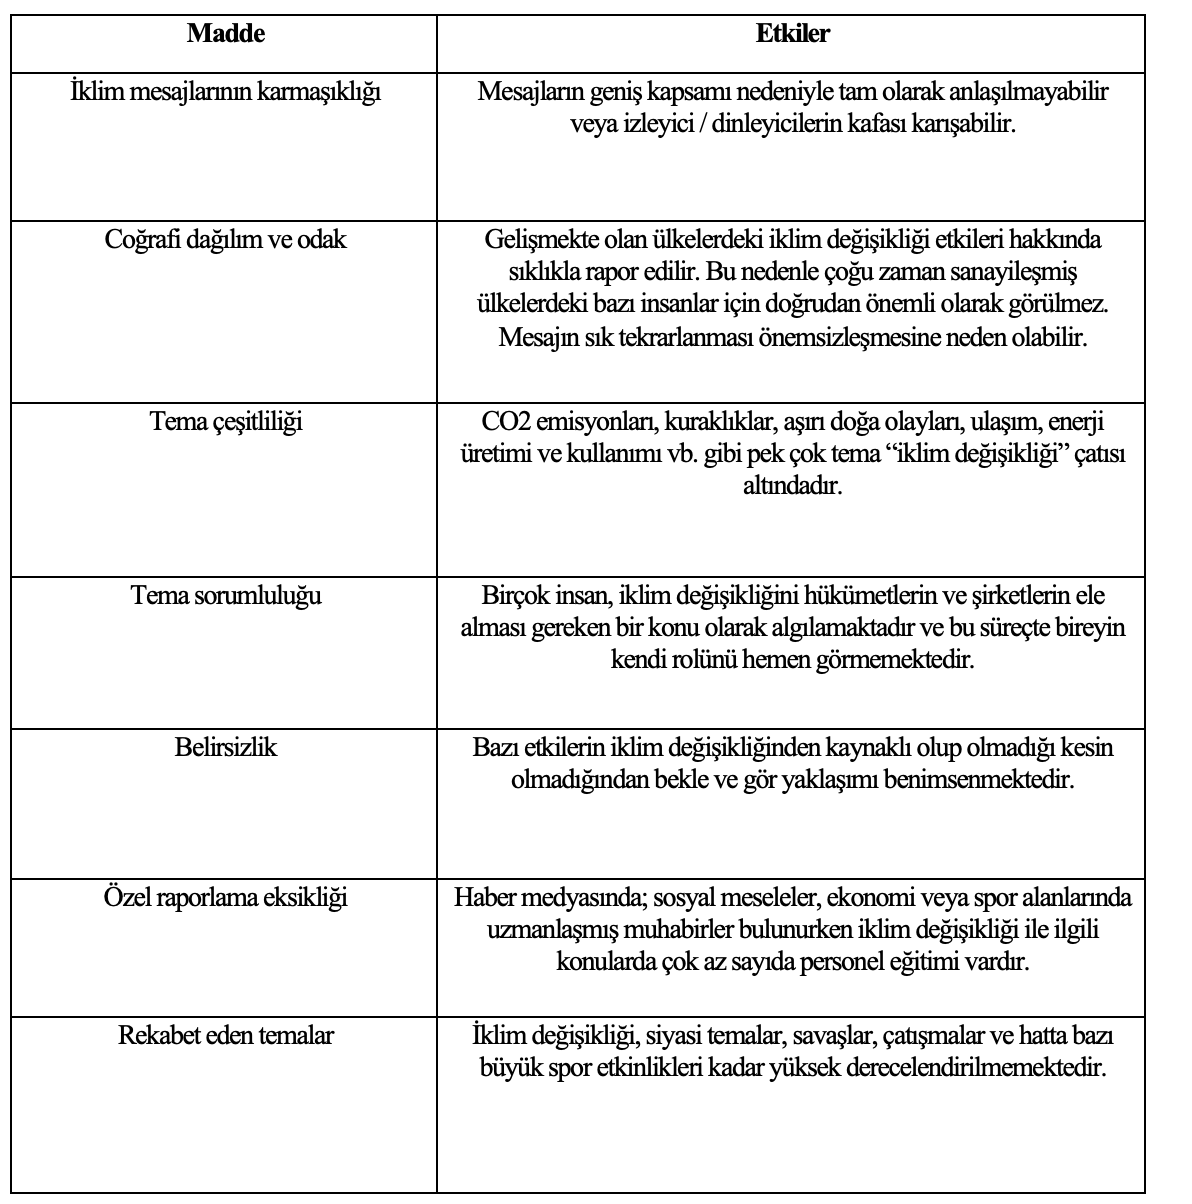
\includegraphics[width=0.95\linewidth,height=0.95\textheight]{tablolar-sekiller/tablo-3-1} \caption{Kaynak: (Mavimbela ve diğerleri, 2018: 42)}\label{fig:unnamed-chunk-3}
\end{figure}

İklim değişikliği, çoğu insanın ilk elden kavrayamadığı ``göze batmayan'' bir konudur (Rogers ve Dearing, 1988). Bu birkaç nedenden kaynaklanmaktadır. Birincisi, iklim değişikliği genellikle büyük zamansal ve mekânsal ölçeklerde tanımlanır; Dünya Meteoroloji Örgütü yalnızca en az 30 yıllık ortalama hava durumu göstergelerine atıfta bulunulduğunda iklimden söz etmeyi önermektedir ve mekânsal olarak iklim çoğunlukla tüm kıtalar, yarım küreler veya tüm dünya için tanımlanır. Çoğu insan için bu tür boyutlar onların yaşam dünyalarının ve biyografik ufuklarının çok ötesindedir. \citep{schaefer2014media}

\hypertarget{iklim-deux11fiux15fikliux11fi-eux11fitimi}{%
\subsection{İklim Değişikliği Eğitimi}\label{iklim-deux11fiux15fikliux11fi-eux11fitimi}}

İklim değişikliği iletişiminin kitleleri eğitmek ve bilgilendirme görevinin yanı sıra; iyi bir iletişim stratejisiyle çok daha fazlası başarılabilir. Filho iyi bir iklim iletişim stratejisinin şu sonuçlara ulaşabilmesini belirtmiştir (s. 4). \citep{leal2019overview}

• İnsanları, iklim krizinin kendi çevreleri için oluşturabileceği riskler hakkında bilgilendirilmelidir. Küresel olan ancak etkileri yerelde de görülen riskleri, daha küresel bir kriz durumunu algılamaktan daha etkili olacaktır.

• Bireylerin kendi ülke politikalarının ve kendi davranışlarının iklim krizini nasıl etkilediği üzerine düşünmesini sağlanmalıdır: Örneğin; su kullanımı, enerji kullanımı, ulaşım gibi günlük yapılan rutinlerin iklim krizinin farkında olarak akıllı ve uygun bir şekilde kullanılmasını teşvik etmek.

Dünya çapında bazı devlet kurumları ve uluslararası kuruluşlar tarafından bugüne kadar gerçekleştirilen iklim çabaları yukarıdaki Tablo 3.1'de özetlenen bir ya da daha fazla faktörü göz ardı ettiğinden mesajların etki derecesi sınırlı kalabilmektedir. Tutum ve davranışlardaki değişikliğin teşvik edilmesi, bir günde veya yalnızca bir faktöre odaklanılarak elde edilemez. İklim kriziyle ilgili konularda halkın / bireylerin tam katılımının sağlanması için; bilgilendirme, eğitim, teşvik etme, izleme bileşenleri dikkate alınmalıdır. İklim iletişim süreçleri genellikle ``bilgilendirme'' ve ``eğitim'' bileşenlerine odaklanırken, ``teşvik etme'' ve ``izleme'' bileşenleri nadiren göz önünde bulundurulmaktadır. İklim iletişim süreçlerinin başarısı için ``izleme'' bileşeninin de eklenmesi önem arz etmektedir (s. 5). \citep{leal2019overview}

Almanya'daki Hamburg Uygulamalı Bilimler Üniversitesi tarafından 2018 yılında kurulan Uluslararası İklim Değişikliği Programı (ICCIP) (Leal Filho, Lackner ve McGhie, 2019: 5-6) iklim değişikliği hakkında bilgi ve iletişimi teşvik etmek için aşağıdaki maddeleri önermektedir.

• İklim değişikliğiyle ilgili çevresel, sosyal, ekonomik ve politik yönleri de dahil olmak üzere kitap, kitap bölümleri, bilimsel dergi makaleleri gibi bilimsel araştırmaların, uzman olmayan bireyler tarafından anlaşılmasına yönelik bir dil kullanılması gerektiği.

• Birleşmiş Milletler kurumları, üniversiteler, bilim kurumları, devlet kurumları, sivil toplum kurumları ve diğer paydaşlarla iş birlikleri gerçekleştirmek. Gelişmiş ve gelişmekte olan ülkeler arasında iklim değişikliği konularında eğitim, iletişim ve bilinçlendirme, farkındalık projeleri yürütmek.

• İklim iletişimiyle ilgili problemler, engeller, zorluklar, fırsatlar ve potansiyelleri tartışmanın yollarını bulmak.

\textbf{Tablo 3.2:} İklim Değişikliği İletişim Girişimleriyle Ulaşılacak Hedef Kitlelerden Bazıları.

\begin{figure}
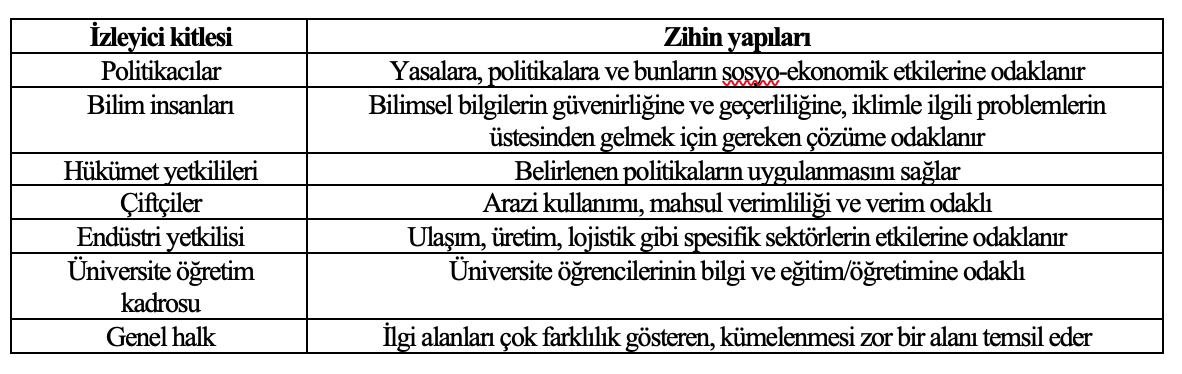
\includegraphics[width=0.95\linewidth,height=0.95\textheight]{tablolar-sekiller/tablo-3-2} \caption{Kaynak: (Mavimbela ve diğerleri, 2018: 42)}\label{fig:unnamed-chunk-4}
\end{figure}

Tablo 3.2, iklim değişikliği kapsamında en önemli hedef gruplarını genel olarak çerçevelemek için hazırlanmıştır. Bu listeye başka gruplarda eklenmesi mümkündür. Bu tablo, hedef gruplarının iklim değişikliğiyle ilgili açılarını betimlemekte; onların potansiyellerinin, eylemlerinin, katılımlarının iyi anlaşılmasına ve kapsamını açıklamaya yardımcı olmaktadır.

Genel halk sınıflandırması, iklim değişikliğine yönelik toplumsal destek oluşturmadaki gri alanı temsil etmektedir. Çünkü her bir bireyin zihinsel çerçeveleri ve kişisel ilgi alanları çok geniştir. Bu belirsiz gruplar için iklim iletişim planı oluşturmak diğer gruplara göre daha zor olacaktır.

İklim değişikliği gerçeği farkından eyleme geçme niyetini ölçen çalışmalarda yapılmıştır. İklim değişikliği literatüründe farkındalığın somut eyleme dönüşmesiyle ilgili yapılan çalışmada Prochaska'nın davranışsal değişim aşaması modeli kullanılmıştır. Araştırma, iklim değişikliğiyle ilgili bilginin iletme ve eyleme geçirmek için duyguların ve biliş mekanizmalarının göz önünde bulundurulması sonucu ortaya çıkmıştır. \citep{trolliet2019awareness} Değişim, birkaç aşamadan oluşan dinamik bir süreçtir. Tutum, davranış ve düşüncelerimizle birlikte davranışlarımızda zaman içerisinde değişmektedir. Prochaska ve Diclemente ``Transtheorical model of change'' adında \citep{prochaska1983stages}, 1) karar öncesi ön düşünme, 2) derin düşünme, 3) hazırlık, 4) eylem, 5) devam ettirme, 6) tekrarlamak ya da son bulma / tamamlama, bu altı basamaktan oluşan modeli geliştirdiler.

\textbf{Tablo 3.3:} İklim İletişiminde Tarihsel Aşamalar ve Bireysel Davranış Değişikliğinde Buna Karşılık Gelen Analoji.

\begin{figure}
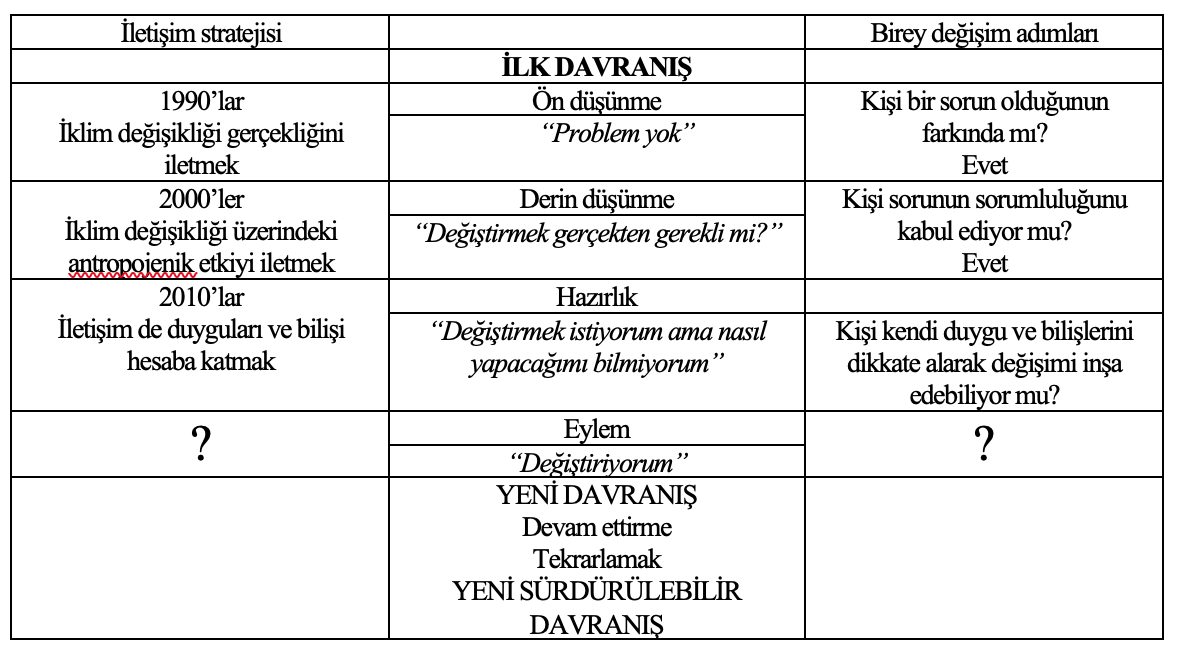
\includegraphics[width=0.95\linewidth,height=0.95\textheight]{tablolar-sekiller/tablo-3-3} \caption{Kaynak: (Mavimbela ve diğerleri, 2018: 42)}\label{fig:unnamed-chunk-5}
\end{figure}

Birinci aşama `ön düşünme' (1) aşamasında genelde insanlar davranışlarını değiştirmeyi düşünmezler ve çoğu zaman davranışlarında herhangi bir sorun olduğunun da farkında olmazlar. İkinci aşamaya geçmek için burada bilgi ve farkındalık yaratmaya ihtiyaç vardır. `Ön düşünme', insanları iklim değişikliğinin gerçek bir fenomen olduğuna inandırma ve onları ikna etme aşamasıdır. Bu aşama 1990'lı yılları kapsamaktadır. Bu iletişim çabasının sembolik başlangıç noktası 1988'de IPCC'nin kurulmasıdır.

Derin düşünme (2) kararsızlık aşaması olarak tanımlanmaktadır. Bireyler sorunun farkındadırlar, değişmeyi düşünürler, fakat sorundan kişisel olarak sorumlu hissetmezler. Son 20 yılda iklim değişikliğiyle ilgili yeni iletişim uygulamaları yapılmıştır. İklim değişikliğiyle ilgili farkındalık oluşturmakla başlandı, sonrasın da iklim değişikliğine antropojenik katkıyı oluşturma ve onu iletmeye geçilmiştir.
Hazırlık aşaması (3), bireyler kararlı bir şekilde değişime karar verdiklerinde bu aşamaya girerler. Gerekli eylem tarzını değiştirmeye ve planlamaya niyetlidirler.

Trolliet ve arkadaşlarının çalışmasında (2019) bu aşamada olduğumuz vurgulanmaktadır.
İklim değişikliğinin odaklanması gereken ana kitlelerden bir tanesi gençlerdir. Çünkü iklim değişikliğinden önceki nesillere göre daha çok etkilenecektir. Almanya ve Avusturya'da 13-16 yaş grubu arasında 760 kişi üzerinde yapılan çalışmada iklim değişikliği farkındalığının çeşitli yönlerinde farklılık gösteren dört farklı genç grubunu belirlenmiştir. Bir grup genç insanın iklim değişikliğiyle ilgili endişe duymadıklarını ve iklim dostu bir şekilde hareket etmeye istekli olmadıklarını ortaya çıkartmıştır. İklim değişikliğiyle ilgilenmeyen gençlerin, iklim değişikliğinin gelecekte olacağına inandıkları, fakat harekete geçmeye istekli olmayan bir grup genç ise iklim değişikliğine yönelik kendi etkilerini sorguladığı gözlemlenmiştir (Alina, Annemarie, Johann, Lars ve Anna, 2019). Diğer bir çalışmada, üniversite öğrencilerinin iklim değişikliği ve çevre sorunları üzerine farkındalıklarının ölçüldüğü çalışmada (n: 471), öğrencilerin çevre sorunlarına yönelik tutumları ile iklim değişikliğine yönelik algıları arasında pozitif yönlü, orta düzeyde anlamlı bir ilişki olduğu ortaya çıkmıştır. Çevre sorunlarına yönelik tutumlarının artmasının iklim değişikliğine yönelik algılarını da arttırdığı belirlenmiştir (s. 667). \citep{sen2018universite} Bir sonraki aşamaya geçmek için insanların sadece bilgi düzeyini değil, aynı zamanda sorunları düşünme ve hissetme biçimlerini de dikkatte alınması gerektiği belirtilmektedir. Trolliet ve arkadaşlarının \citep{trolliet2019awareness} çalışmasında, eyleme geçmenin önündeki bilişsel ve duygusal engelleri dikkate alan bir iletişim stratejisi analizi de önerilmiştir.

Eylem aşamasında (4), insanlar davranışlarında önemli değişiklikler yapmışlardır. Kendini yeniden değerlendirme, kendini özgürleştirme, yardımlaşma ilişkileri gibi değişim süreçleri bu aşamada aktiftir.

Devam ettirme (5) davranış değişiklikleri artık sabittir. İnsanlar geliştikleri ve değişimi mümkün kılmaya devam ettikleri gerçeğinden emindirler.

Sonlandırma / bütünleşme aşaması (6), bu aşamada insanlar tekrarlayabilir ya da başa dönebilir. Tekrarlamak başlangıç noktasına geri dönme anlamına gelmemektedir. Kendi içinde bir öğrenme süreci ve doğrusal olmayan, dinamik değişim süreci içinde bir evrim olabilir (s. 51). \citep{trolliet2019awareness}

Parry ve arkadaşları iklim finansmanı üzerine hazırlamış oldukları çalışmada daha önce yapılan finansal tahminlerdeki belirsizlikleri göstermeye çalışmışlardır. Düşük tahmin nedenleri olarak şunları belirtmektedirler (s. 7). \citep{parry2009assessing}

\begin{enumerate}
\def\labelenumi{\arabic{enumi})}
\item
  Bazı sektörler maliyet değerlendirmesine dahil edilmemişlerdir. Örneğin; ekosistemler, enerji, imalat, perakendecilik, turizm.
\item
  Dahil edilen bu sektörlerden bazıları kısmen kapsanmıştır.
\item
  Adaptasyonun ek maliyetleri bazen düşük varsayılan yatırım seviyelerine karşı `iklim artışları' olarak hesaplanmıştır.
\end{enumerate}

İklim maliyetlerinde hasarların da değerlendirilmesi ve raporlanması gerektiğinin altı çizilmektedir. Çünkü teknik ve ekonomik kısıtlamalar nedeniyle tüm hasarlar önlenemez. Gelişmekte olan ülkelerin ihtiyaç duyduğu mali yardımın iki ve üç katı olduğu, özel sektörler için bunun çok daha fazla olduğu belirtilmektedir. \citep{parry2009assessing} İklim finansmanıyla ilgili literatürde; iklim değişikliği uyumuyla ilgili üç özel konunun ele alınması önerilmektedir. Daha yenilikçi finansal mekanizmaların bulunmasını, özel sektörün iklim uyum sürecine dahil edilmesini ve uyum fonlarının etkin bir şekilde kullanılmasını kapsamaktadır (s. 43). \citep{roy2018evaluating}

\hypertarget{iklim-deux11fiux15fikliux11fi-yuxf6netiux15fimi}{%
\section{İklim Değişikliği Yönetişimi}\label{iklim-deux11fiux15fikliux11fi-yuxf6netiux15fimi}}

İklim kriziyle sorunların ve problemlerin çözülmesi adına; ülkeler hem kendi içlerinde hem de birbirleriyle yönetişim mekanizması geliştirilmesi yönünde politikalar yapmak zorundadır. Yönetim sistemleri iklim krizini ve iklim uyum konularını ele almak için tekrardan yapılandırılmalıdır.

İklim değişikliğini ele almak; özellikle enerji, tarım ve ulaşım gibi kilit sektörlerdeki üretim ve tüketim uygulamaları açısından bugünkü işlerin yapılma şeklini değiştirmek anlamına gelmektedir. İklim değişikliği yönetişimi; hükümetlerin, aktif bir azaltma ve uyum politikası rejiminin uygulanmasından yana istikrarlı toplumsal çoğunlukların sürdürülebilmesi için çıkar algılarında değişiklikler meydana getirmede aktif bir rol üstlenmesini gerektirmektedir. Bu tür bir değişimi gerçekleştirmek için yardımcı olabilecek önlemler şunları içermektedir: değişim için koalisyonlar kurmak, muhalifleri satın almak, yeni ekonomik güç merkezleri oluşturmak, yeni kurumsal aktörler yaratmak, yasal hak ve sorumlulukları ayarlamak, fikirleri ve kabul edilmiş normları ve beklentileri değiştirmek. \citep{meadowcroft2009climate}

İklim finansmanının yönetişimi üzerine kavramsal araştırmaların eleştirel bir incelemesi yapılan bir çalışmada, iklim finansmanı sağlayan kurumsal düzenlemeler ve yönetişimi üzerine yeni merkezi olmayan, çok merkezli yapıların, iklim finansmanının iklim değişikliği yönetimini en doğrudan uygulayan devlet içi ve devlet dışı aktörlere daha etkin bir şekilde ulaşmasını sağladığı ifade edilmiştir. \citep{bracking2021climate}

Mevcut yönetişim mekanizmalarında zorluklara neden olan iklim değişikliği sorunuyla ilgili bazı özellikler şunlardır (s. 4). \citep{meadowcroft2009climate}

\textbf{Toplumsal erişim:} Sera gazları, son iki yüzyılda yükselen yaşam standartlarını sürdüren endüstriyel ve tarımsal faaliyetlerle ilişkilidir. Fosil yakıtlar hala küresel birincil enerjinin büyük bir kısmını sağlamaktadır. Mevcut üretim ve tüketim kalıplarının emisyonları önemli ölçüde azaltacak şekilde dönüştürülmesini ve iklim ısınmasına yönelik gerekli uyarlamaların yapılmasını gerektirmektir. Toplumsal uyumun sağlanması bilinçli bir şekilde yönlendirilmelidir.

\textbf{Bilimsel belirsizlik:} İklim değişikliğini yönlendiren süreçler ve insan toplumları üzerindeki etkileri hakkında artık çok şey anlaşılsa da büyük belirsizlikler halen devam etmektedir. Özellikle iklim sisteminin duyarlılığı (atmosferik sera gazı konsantrasyonlarındaki belirli bir artıştan ne kadar ısınmaya yol açacağı); bölgesel iklim etkileri ve ekosistemler için sonuçları neler olacaktır. Bilgi sürekli artsa da öngörülebilir gelecek için belirsizlikler devam etmektedir.

\textbf{Dağıtım ve eşitlik bağlantıları:} İklim değişikliği farklı grupları farklı şekillerde etkileyecektir. Bu etkilerin bazıları tahmin edilebilirken, diğerleri belirsizliğini korumaktadır. İklim değişikliği; ülkelerin, bölgelerin, endüstrilerin, sosyal tabakaların ve bireylerin maruz kaldığı risk ve fırsat kalıplarını değiştirmektedir. Eşitlik sorunları (yerli ve uluslararası) hükümetler için her zaman başa çıkılması en zor konular arasında olmuştur. Yerleşik kaygılar, bölgesel eşitsizlikler, Kuzey/Güney gerilimleri, yakıt yoksulluğu gibi boyutları bulunmaktadır.
\textbf{Uzun zaman dilimleri:} Fosil yakıtların yanmasından kaynaklanan sera gazı emisyonları, sanayi devriminin başlangıcından itibaren artmaktadır. İklim sistemi on yıllar, yüzyıllar ve binyıllar boyunca gelişmektedir. İklim değişikliğini yönetmek, bu yüzyıl boyunca bir yönetişim sorunudur. Bu tür uzun vadeli meseleler, dört yıllık bir seçim döngüsüne, bakanların ve üst düzey yetkililerin iki veya üç yıllık görev süresine ve günlük siyasetin günübirlik veya haftalık ritimlerine pek uymamaktadır.

\textbf{Küresel etkiler:} İklim değişikliğinin nedenleri ve etkileri uluslararasıdır. Uluslararasındaki ekonomik ve diğer bağlar, kolektif bir tepkiyi gerekli kılmaktadır. Ancak, uluslararası çabaları bu ölçekte koordine etmek büyük bir zorluk oluşturmaktadır.

\textbf{Şekil 3.3:} Yönetişimin Paydaş ve Araçları

\begin{figure}
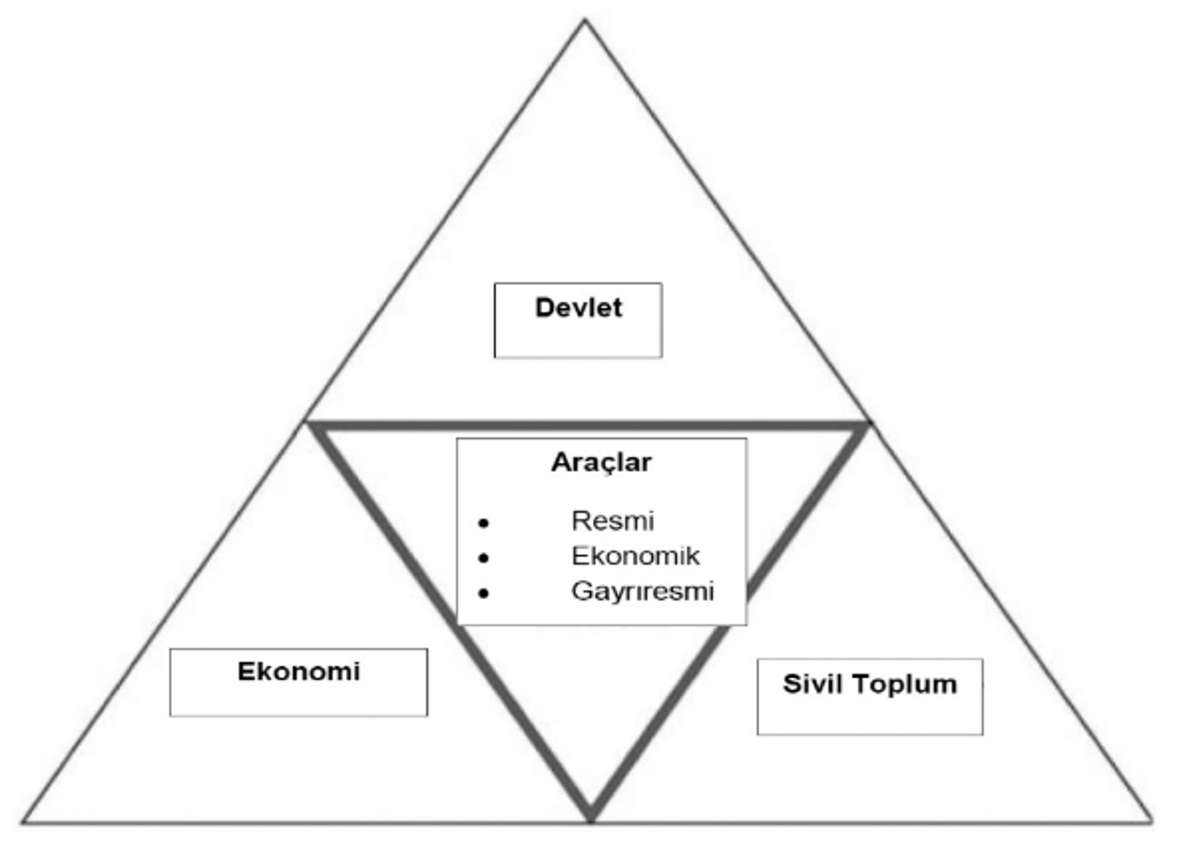
\includegraphics[width=0.95\linewidth,height=0.95\textheight]{tablolar-sekiller/sekil-3-3} \caption{Kaynak: (Mavimbela ve diğerleri, 2018: 42)}\label{fig:unnamed-chunk-6}
\end{figure}

Devlet, yönetişim düzenlemelerinde araçların belirlenmesi, oluşturulması ve uygulanması noktasında tek başına karar alıcı değildir. Sivil toplum örgütleri, özel sektör aktörleri de toplumsal düzenlemelerin kararlarında yer almaktadır. Bu aktörlerin ortak noktası olan araçlar, resmi ya da düzenleyici araçlar (mekân, peyzaj, sektör planlamaları); ekonomik araçlar (vergi ve yardım gibi rekabetçi unsurlar); gayri resmi araçlar (bilgi, katılım, iş birliği gibi araçlar) kapsamaktadır (s. 13-14). \citep{frohlich2013conceptualising}

Literatürde, çevre ve iklim konusunda farklı aktör sınıflandırmaları yer almaktadır. Bu aktörler, bazıları tek bir grupta ele alınmış, bazıları ise daha alt gruplarda ele alınmıştır. ozmen2011cevre ``Çevre İletişimi: Çevre Haberlerinin Yapısal Analizi ve Okuyucu Farkındalığı'' adlı doktora tezinde, çevre iletişimiyle ilgili aktörleri beş ana kategoride sınıflandırmıştır. Bunlar;

1- Medya

2- Vatandaşlar ve Sivil Toplum Kuruluşları (STK)

3- Devlet Kuruluşları

4- İş Dünyası

5- Eğitim Kurumları

\citet{sahin2014turkiye} ise, uluslararası kuruluşları da ayrı bir kategoride değerlendirerek altı ana kategoride iklim aktörlerini ele almıştır. Şahin, Türkiye'deki iklim aktörlerini hükümet ve hükümet dışı olarak iki ana kategoriye ayırmıştır. Devlet ile kamu kurumlarının beraber alınmasının sakıncalarına rağmen, bakanlıklar ve bağlı kuruluşlar, yerel yönetimler ve kanun koyucular (siyaset) kamu kurumları aynı sınıflandırma içerisinde yer almıştır. Ek olarak, kanun ile kurulmuş olan meslek odaları, sanayi ve ticaret odaları, vakıflar kamu kurumları arasına dahil edilmiştir. Hükümet dışı sınıflandırma da ise; sivil toplum kuruluşları (STK), özel sektör, üniversiteler ve medya olarak yer almaktadır. Uluslararası kuruluşlar ise; Birleşmiş Milletler ve diğer uluslararası devletler arası niteliğinden dolayı bu iki grubun arasında yer verilmiştir (s. 64). \citep{sahin2014turkiye}

\textbf{Tablo 3.4:} Aktörlerin Sınıflandırılması.

\begin{figure}
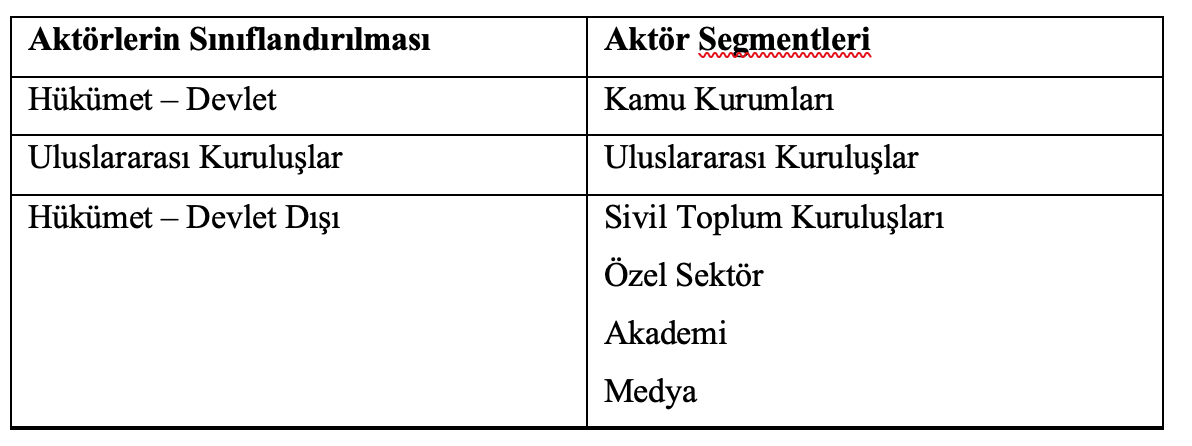
\includegraphics[width=0.95\linewidth,height=0.95\textheight]{tablolar-sekiller/tablo-3-4} \caption{Kaynak: (Mavimbela ve diğerleri, 2018: 42)}\label{fig:unnamed-chunk-7}
\end{figure}

ozer2017iklim, ``İklim Değişikliği Yönetişimindeki Aktörlerin Analizi ve Türkiye'' çalışmasında iklim aktörlerini dört ana sınıfta belirlemiştir. Bunlar; devletler, kentler ve yerel yönetimler, sivil toplum kuruluşları ve bilim insanlarıdır. İklim değişikliğine yönelik temel prensipler Birleşmiş Milletler çatısı altında müzakere edildiğinden dolayı ve bu müzakere de alınan yetki ve sorumlulukların iç politikaya aktarılmasında ana aktör devlet olduğu görülmektedir. İklim değişikliği konusunda imzalanan anlaşmalar her ne kadar uluslararası düzeyde olsa da iklim değişikliğine yönelik yapılacak politika ve eylemler kapsamında her ülkeye ait kamu kurumlarına, akademiye, iş dünyasına ve vatandaşlara büyük ödevler düşmektedir (s. 839). \citep{ozer2017iklim}

\textbf{Şekil 3.4:} İklim Değişikliği Yönetişimi Aktörleri.

\begin{figure}
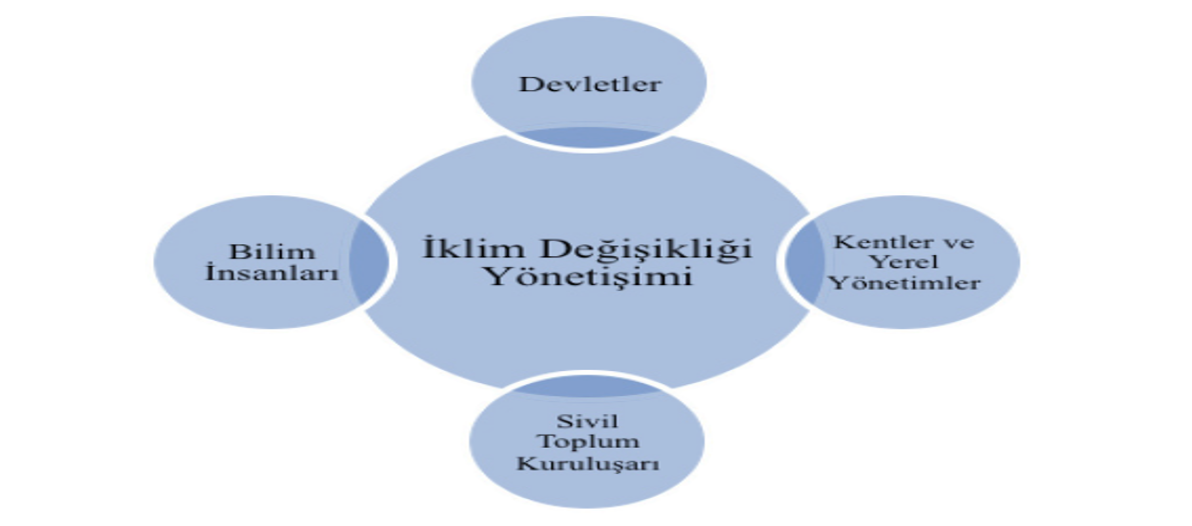
\includegraphics[width=0.95\linewidth,height=0.95\textheight]{tablolar-sekiller/sekil-3-4} \caption{Kaynak: (Mavimbela ve diğerleri, 2018: 42)}\label{fig:unnamed-chunk-8}
\end{figure}

\hypertarget{iklim-aktuxf6rleri}{%
\section{İklim Aktörleri}\label{iklim-aktuxf6rleri}}

İklim krizi global bir sorun olarak tüm dünyayı etkilemektedir. İklim konusu çok aktörlü ve çok düzeylidir. Bu kapsamda, daha önce iklim aktörleri üzerine yapılan çalışmalardan yola çıkarak, iklim aktörleri rol, sorumluluk ve kapasiteleri bakımından ele alınmıştır.

90'lı yıllardan itibaren, dünya ülkeleri, global sorunları çözmek için daha çok görüşmeler yapmıştır. Çevre ve iklim problemleri, küresel nitelikte çözülmesi gereken sorunların başında gelmektedir. Bu nedenle çözümler yine global ölçekte aranmalıdır. Tüm dünya ülkelerini bir araya getiren en önemli çevre konusu, iklim krizidir. Bu kriz, tek bir ülkeyi değil, tüm dünyadaki yaşamı ilgilendiren, sorunun çözülmesine yönelik kalıcı tedbirlerin ve kuralların yer aldığı bir yönetişim modelini zorunlu kılmaktadır. İklim değişikliği yönetişimi, global ölçekte sadece devletlerin değil, devlet dışı tüm aktörlerin de çözümün bir parçası olması talep etmektedir. Bu talep, ulusal düzeyde de devlet dışı aktörlerden aynı şekilde beklenmektedir. Yerel düzeyde iklim değişikliğine yönelik yapılacak çalışmalar için önem arz etmektedir.

İklim değişikliği yönetişim süreçleri, problemlerin çözülmesine yönelik önlemlerin alınmasına yönelik kararlar alınması ve bunların uygulanmasını kapsamaktadır. Bu çok aktörlü ve katmanlı devam eden iklim aktörlerinin rol ve sorumlulukları kadar katılımın sürekliliği de önemlidir. Ancak bu yolla hem küresel hem ulusal düzeyde bir yönetişim modelinin başarısından söz etmek mümkündür. Katılım problemi sahiplenmeyi de beraberinde getirecektir. İklim değişikliği yönetişiminde öne çıkan aktörler; devletler, kentler ve yerel yönetimler, sivil toplum kuruluşları ve bilim insanlarıdır (Özer, 2017). \citep{ozer2017iklim}

İklim aktörleri farklı alanlardan gelmektedir. Bunlar bilimsel, politik, ekonomik, sosyal bilgiye sahip ve iletişim sürecinin oluşması, toplumsal farkındalık, toplumu eğitme ve yönlendirme noktasında medya, kamu kurumları, sivil toplum örgütleri ve iş çevrelerini kapsamaktadır (s. 39). \citep{ozmen2011cevre}

İklim politikaları, iklim krizine neden olan sera gazlarının emisyonlarını azaltmak, bu krize neden olan etmenleri ortadan kaldırmak ve iklim krizi etkilerini en azami şekilde indirgemek için gerekli olan finansmanı ve teknolojiyi geliştirmekle ilgilidir. Fakat bu kriz, tüm üretim ve tüketim biçimleriyle birlikte bu ekonomik sistem içerisinde, başta enerji sektörü olmak üzere ekonomi ve üretim alanında ele alınacak konular iç içe geçmiştir. Bu nedenle enerji, sanayi, tarım, hayvancılık, ormancılık, inşaat gibi sektörlerin bilim, teknoloji ve finans sektörüyle ilgili ortaya konması gereken makroekonomik hedefler ve kararlar iklim kriziyle ilgili alınması gereken aksiyon planlarıyla yakından ilişkilidir. İklim politikalarının ve aktörlerinin bu sınırlar içinde tanımlanması noktasında faydalı olmuştur (s. 64). \citep{sahin2014turkiye}

İklim aktörleri araştırmalarında ufak sınıflandırma farklılıkları gösterse de kapsam olarak benzer oldukları görülmektedir. Bu kapsamda, iklim aktörlerinden medya, sivil toplum kuruluşları, devlet kuruluşları, özel sektör ve eğitim kurumlarına değinilecektir.

\hypertarget{medya}{%
\subsection{Medya}\label{medya}}

Haber medyası, gündem belirleme gücü nedeniyle bilimsel konular, kişiler ve olaylar hakkında önemli bir bilgi kaynağıdır. Medyada yer alan haberler ile halkın tutumları arasındaki ilişki farklılık gösterse de iklim değişikliğinin medyada yer alması konuyla ilgili halkın katılımı tutumunu şekillendirmektedir. \citep{gunay2021media} İklim değişikliği konusuna dikkat çekilmesi açısından geleneksel medya önemini korumaktadır. Çevre ve iklim değişikliğine yönelik farkındalık oluşturulması, kamunun eğitilmesi noktasında, kitle iletişim araçlarının kullanılması, günümüzde de önemini korumaktadır.

Gelişmekte olan ülkelerdeki gazetelerin iklim hareketine yönelik adaptasyonuna veya iklim krizi zararlarının azaltımına yönelik olarak haberlerin çerçevelenip çerçevelemediği araştırılmıştır. Bu kapsamda, Nijerya ve Türkiye gazetelerinin iklim değişikliği haberlerinin karşılaştırılmalı nicel bir analizi gerçekleştirilmiştir. Çalışma sonucunda; iklim eylem çerçevesinde çıkan haberlerin, Nijerya'da adaptasyona yönelik çerçevelerin daha baskın olduğu, Türkiye'de ise adaptasyon ve azaltıma yönelik çıkan haberlerin birbirine yakın olduğu sonucu ortaya çıkmıştır. \citep{gunay2021media}

Türkiye'de iklim konusunda yayın yapan medya kuruluşları Açık Radyo, National Geographic Dergisi, Atlas Dergisi, İz TV ve Yaban TV çevre ve ikim konularında farkındalık yaratmaktadır (s. 39). \citep{ozmen2011cevre} Alternatif medya olarak, iklim aktörleri daha fazla insana ulaşmak, çevre ve iklim konularına dikkat çekmek için Youtube, Instagram, Spotify gibi platformlarda da içerik üretmektedirler. Bunların başında TEMA Vakfı, Yeşil Gazete, National Geographic Türkiye Youtube kanalları yer almaktadır.

Şahin ve Üzelgün'ün Türkiye'de iklim değişikliğinin geleneksel medya gündemine taşınmasına dair gazete yöneticileriyle yapmış oldukları mülakatlar sonucunda, iklim değişikliğini önemli bulmakla birlikte, şartlar nedeniyle yeterince bu konuyu gündeme getirmediğini belirtmişlerdir. Türkiye gündeminin ekonomik ve politik nedenlerle yoğun olması, medya okurlarının ve izleyicilerin dikkatini çekmediği, iklim değişikliğinin gelecekle ilgili soyut bir konu olması, Türkiye'nin aktif iklim politikalarına sahip olmadığından dolayı kamunun ve medyanın iklim haberlerine dair gündem yaratamaması, aşırı hava ve iklim olaylarıyla ilgili haberler yapılırken iklim değişikliğiyle ilgili bağlantıların yeterince yapılmadığı gibi durumların olduğu tespit edilmiştir (s. 14). \citep{sahin2016iklim}

Son dönemde, sıcaklıkların artması, 2021 Türkiye'deki orman yangıları gibi çevre felaketlerinin artması ve insanların bu olguyu tecrübe etmeleri neticesinde hem geleneksel medya hem de alternatif medya da iklim ve çevre konularıyla ilgili içerikler yer almaktadır. Facebook, Twitter ve Instagram gibi sosyal ağlar neticesinde, çevre ve iklim konularında insanlar bir tartışma ortamı oluşturabilmekte ve bunun da çevre ve iklim konularına dair farkındalığı arttırdığı ve eyleme geçilmesi noktasında hem kamulara hem de sadece vatandaşlar noktasında bir baskı unsuru yarattığı ifade edilebilir.

İklim değişikliği iletişimi üzerine literatürde artan bir eğilim, olumlu, ileriye dönük mesajlaşmanın etkili eylemi motive etmenin yolu olduğunu göstermektedir. Bununla birlikte, aşırı hava olaylarıyla ilgili faydalı olmayan anlatıları da güçlendirmeye yönelik olarak duyarlı olduğu belirtilmektedir. Medyada hava olaylarıyla ilgili söylemler olumsuz kalıpları takip etme eğilimindedir. Psikologlar ve sosyal bilimciler tarafından yapılan araştırmalar, olumsuz ifadelerin fazla vurgulanmasının takipçilerde çaresizlik, yararsızlık duygularını veya iklim değişikliğini inkâr etme motivasyonunu artırdığını göstermektedir. Araştırmalar olumsuz sonuçlardan ziyade olumlu olasılıkları vurgulayan mesajların takipçilerin dikkatini çektiğini, kendi davranışlarını değiştirme motivasyonlarını arttırdığını ve iklim değişikliğiyle uyumlu eylemleri desteklediğini vurgulamaktadır. Korkunç bir çevre ya da iklim portresi çizmek yerine gelecek için birlikte inşa edebileceğimiz temiz, daha güçlü bir dünya anlatısı yararlı olacaktır. İklim değişikliği temalarının kişiselleştirilmesi, yerelleştirilmesi gerektiği, bunu yaparken de fedakârlık ve iş birliği gibi temaların işlenmesi gerektiği ifade edilmektedir. Bu noktada hangi hedef kitlelerin hedeflenmesi ve hangi özel mesajların, içeriklerin kullanılması gerektiği konusunda bölgesel, yerel araştırmalar yapılmalıdır. \citep{munger2019avoiding}

İklim değişikliğinin toplumsal önemi, bilim insanları ve halk arasında daha doğrudan bir iletişim ihtiyacını ortaya çıkarmıştır. Hakemli bilimsel makaleler geniş bir kitlenin ilgisini çekmek için pek uygun değildir. Bu da iklim krizinin önemini iletmek için farklı iletişim kanallarını keşfetme ihtiyacını artırmaktadır. Sosyal medya, kitlelerle iletişim kurmak için interaktif bir kaynaktır. Özellikle, bloglar iklim kriziyle ilgili bulguları farklı iletişim seviyelerinde yaymak için kullanışlı bir kaynaktır. Çünkü daha anlaşılır ve bilimsel yayınlara kıyasla daha geniş bir hedef kitleyi hedeflerler. \citep{purath2019blogging}

Antropojenik iklim değişikliğinin etkileri sürekli artarken, kamuoyunun endişesi aynı şekilde artmamaktadır. İklim değişikliği algısı yavaş bir şekilde toplum nezdinde kabul görmektedir. Bu zorluğa rağmen, iklim değişikliğine olan kamu ilgisi ve algısı kritik öneme sahiptir. Bilgilenilmemiş, farkındalığı olmamış bir toplum olmadan, hükümetler, bilim insanları ve kuruluşlar bu krizin etkilerini azaltmakta yetersiz kalacaklardır (s. 130). \citep{purath2019blogging} İklim değişikliğiyle ilgili kamuoyu farkındalığı üzerine 2016 yılında yapılan bir çalışmada Almanlar'ın \%16'sı ve İngilizler'in \%14'ü ikim değişikliğinin insan faaliyetlerinden kaynaklandığına yönelik şüpheci kaldıkları veya iklim değişikliğine inanmadığını belirtmiştir. Açık uçlu bir soruda katılımcıların \%3'ten daha azı her iki ülkede de önümüzdeki 20 yıl içerisinde karşılaşacağı en zorlu problemlerden biri olarak iklim değişikliğini belirtmiştir. \citep{steentjes2017european} Gelişmiş ülkelerde dahi iklim değişikliğinin gelecekteki olası etkilerine yönelik farkındalığın yetersiz olduğu görülmektedir.

\hypertarget{sivil-toplum-kuruluux15flarux131}{%
\subsection{Sivil Toplum Kuruluşları}\label{sivil-toplum-kuruluux15flarux131}}

``Sivil toplum kuruluşları'' (STK) terimi, Birleşmiş Milletler tarafından ikinci dünya savaşı sonrasında kullanılan bir ifadedir. 1945 yılında Birleşmiş Milletler (BM) şartları kabul edildiğinde, sivil toplum kuruluşlarının sorunların çözümünde BM'e danışmanlık yapmaları öngörülmüştür. 1980 yıllarından itibaren, STK terimi BM çerçevesi dışında da kullanılması yaygınlık kazanmıştır. Ulusal ve uluslararası düzeyde faaliyet gösteren her türden toplumsal aktör için kullanılmaya başlanmıştır. Kavram, akademisyenler kadar kendisini aktivist olarak tanımlayanlar tarafından da benimsenmiştir (s. 271-272). \citep{martens2002mission} Bir diğer tanım, STK'ları ``ticari amaçlardan ziyade öncelikle insani veya iş birliğine dayalı amaçlarla karakterize edilen'' özel kuruluşlar olarak tanımlamaktadır (s. 74). \citep{werker2008nongovernmental} STK'lar gelişmekte olan ülke insanlarına yardım etmek, yoksul insanlara sosyal yardım sağlamak, toplumsal kalkınmaya katkıda bulunmak, çevreyi korumak, belirlenen konularda toplumsal bilinci artırmak gibi farklı alanlarda görevler üstlenmektedirler.

Yapılan araştırmalar göstermektedir ki, sivil toplum kuruluşlarına katılım ile demokrasi arasında pozitif yönde korelasyon olduğunu göstermektedir. Yani sivil toplum örgütlerine katılım ne kadar fazlaysa, demokrasinin benzer oranda geliştiği görülmektedir. Sivil toplum kuruluşlarına katılım üzerine yapılan araştırma sonuçlarına göre; Türkiye'de sivil toplum kuruluşlarına üyelik düşük düzeydedir. Yapılan analiz sonucunda Türkiye'de bireylerin sivil toplum kuruluşlarını demokrasinin önemli bir öğesi olarak görmediği, Türkiye'de sivil toplum ve devlet ilişkilerinin olumsuz geçmişinden dolayı bireylerin STK'lar hakkında olumsuz yargılara sahip olduğu ve bundan dolayı üyelikten kaçınmalarına neden olduğu sonucu ortaya çıkmıştır (s. 405). \citep{sahin2019turkiye}

Sivil toplum kuruluşları için iletişim faaliyetleri hayati bir öneme sahiptir. Kamu bilinci, ilgisi ve desteği olmadan bu organizasyonlar var olamazlar (s. 20). \citep{schoenfeld1981environmental} Türkiye'de yerel ve ulusal olarak farklı büyüklükte STK'lar faaliyet göstermektedir. 2021 yılı itibariyle Türkiye'de faaliyet gösteren STK sayısı 122.068'dir. Konumuzla alakalı olarak; ``Çevre Doğal Hayat Hayvanları Koruma Dernekleri'' 2.638, ``Gıda, Tarım ve Hayvancılık'' dernekleri 819, ``İmar, Şehircilik ve Kalkındırma'' dernekleri 1.636'dır.

\textbf{Şekil 3.5:} Derneklerin Faaliyet Alanların Göre Dağılımı

\begin{figure}
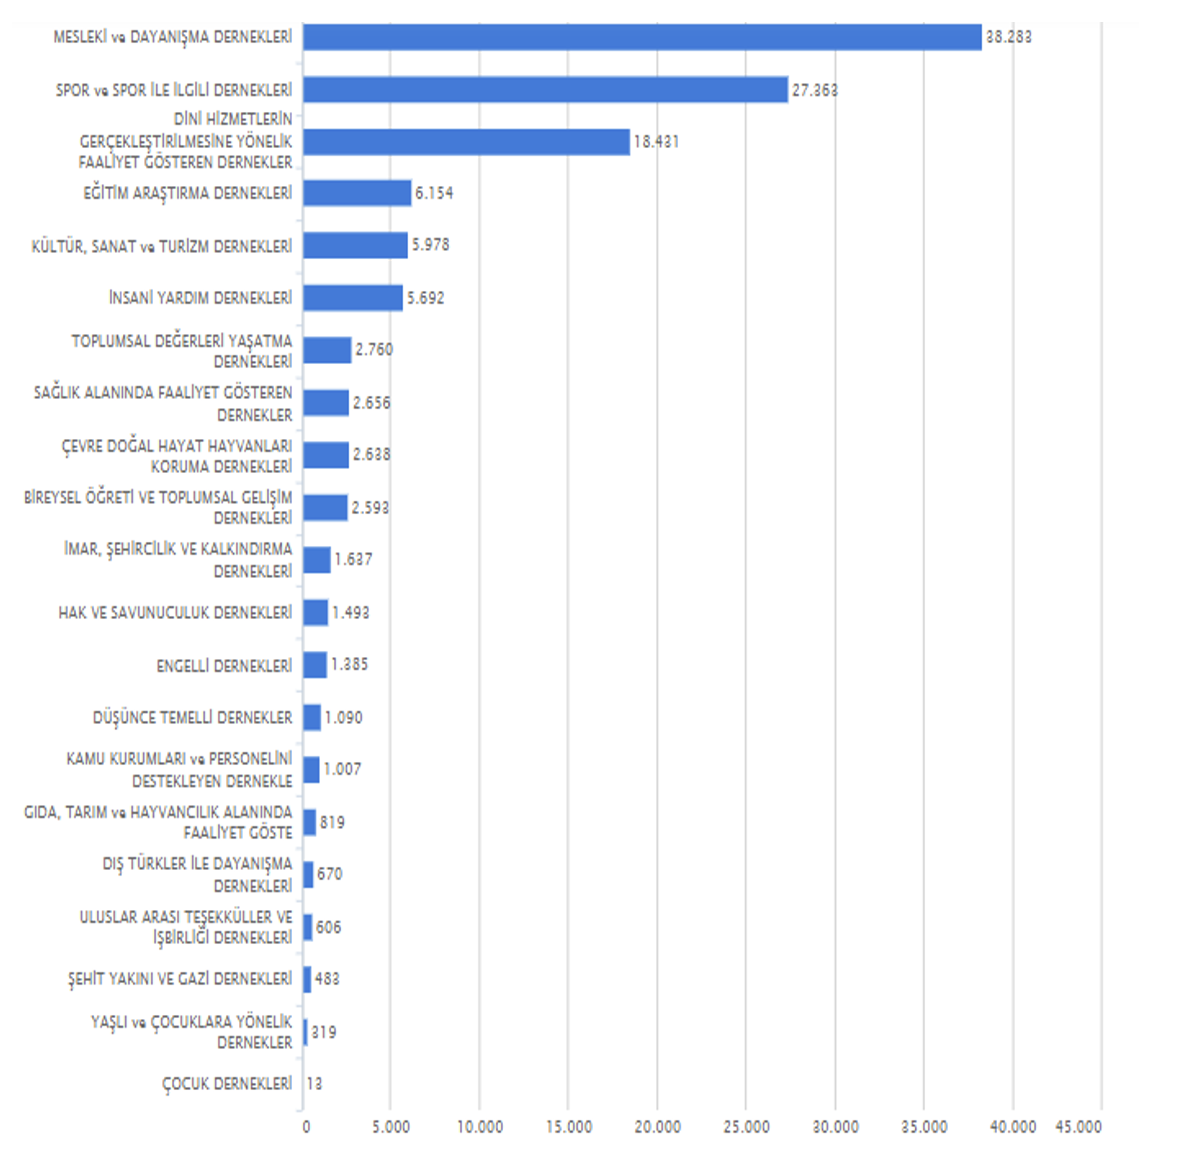
\includegraphics[width=0.95\linewidth,height=0.95\textheight]{tablolar-sekiller/sekil-3-5} \caption{Kaynak: (Mavimbela ve diğerleri, 2018: 42)}\label{fig:unnamed-chunk-9}
\end{figure}

\hypertarget{devlet-kuruluux15flarux131}{%
\subsection{Devlet Kuruluşları}\label{devlet-kuruluux15flarux131}}

İklim krizinin en önemli aktörlerinden biri de devlet kuruluşlarıdır. Bu kapsamda, bakanlıklar ve belediyeler ele alınmaktadır. İklim krizi hakkında farkındalığın artması, toplumsal davranış değişikliklerinin oluşturulması, çevre bilinçlendirilmesi, çevre gündeminin belirlenmesi gibi konularda bazı kamu kurum ve kuruluşlarının yasama, yürütme, denetleme gibi yetkilerinden ve devlet imkanlarından daha kolay yararlanma bakımından diğer aktörlere göre daha etkili olduğu ifade edilebilir.

Türkiye'de çevre konusunda çalışmalar Çevre ve Şehircilik Bakanlığı, Tarım ve Orman Bakanlığı tarafından yürütülmektedir. Çevre ve Şehircilik Bakanlığı bünyesinde; ``Çevre Yönetimi Genel Müdürlüğü'', ``İklim Değişikliği ve Hava Yönetimi Koordinasyon Kurulu'' bulunmaktadır. Tarım ve Orman Bakanlığı bünyesinde ``Su Yönetimi Genel Müdürlüğü'', ``Devlet Su İşleri (DSİ) Genel Müdürlüğü'', ``Meteoroloji Genel Müdürlüğü (MGM)'', ``Orman Genel Müdürlüğü (OGM)'' bulunmaktadır.

\citet{sahin2014turkiye}, iklim aktörleri çalışmasında (2014) Kalkınma Bakanlığı'nı, şimdiki adıyla ``Strateji ve Bütçe Başkanlığı, Dışişleri Bakanlığı, Enerji ve Tabi Kaynaklar Bakanlığı, Ulaştırma ve Altyapı Bakanlığı (Çalışmada geçen eski adı: Ulaştırma, Denizcilik ve Haberleşme Bakanlığı), Sanayi ve Teknoloji Bakanlığı (çalışmada geçen eski adı: Bilim, Sanayi ve Teknoloji Bakanlığı), Avrupa Birliği Bakanlığı, Maliye Bakanlığı, Ticaret Bakanlığı (çalışmada geçen eski adı: Ekonomi Bakanlığı) iklim aktörleri arasında ele almıştır.

Hanelerin, küçük sanayi merkezlerin ve işletmelerin elektrik tüketimleri, aydınlatma, ısıtma-soğutma, atık ve şehir ulaşımı gibi faktörler şehirlerde önemli ölçüde sera gazı emisyonuna neden olmaktadır. İklim krizine yönelik olarak, şehirciliğin kuramsal yapıları bugün tekrar sorgulanmaktadır. Enerji, inşaat, ulaşım, atık olmak üzere şehri oluşturan unsurların yönetimi yeniden iklim krizi kapsamında ele alınmalıdır. Bu doğrultuda, şehirlerin yönetimi ve planlamasından sorumlu yerel yönetimler önem kazanmaktadır (s. 7-8). \citep{talu2019iklim}

Hükümetlerin, iklim değişikliğini azaltma ve ona uyum sağlamadaki rolüne ilişkin çok sayıda çalışma yapılmıştır. Hükümetler, yükümlülük sahipleri olarak ülkelerin çevresel, ekonomik, sosyal ve diğer kırılganlıklarını ele almak için eylemler düzenlemesi beklenmektedir (s. 81). \citep{fe2019philippine}

\hypertarget{uxf6zel-sektuxf6r}{%
\subsection{Özel Sektör}\label{uxf6zel-sektuxf6r}}

Çevreye duyarlılığının toplum nezdinde artmasıyla birlikte, iş dünyası üretim modellemelerinde çevre dostu ürünlere ve hizmetlere yönelmişlerdir. Aynı zamanda, iş dünyasının çevre ve iklim konularında yaptığı çalışmalar nedeniyle toplumun bu konulara yönelik farkındalığı artmaktadır. Özellikle, şirketlerin bu temalarda yaptıkları faaliyetler, yeşil pazarlama, sosyal sorumluluk, halkla ilişkiler gibi uygulamalar içerisinde yer almaktadır.

Özel sektörün iklim krizine ilişkin farkındalığın artması için TÜSİAD ve REC Türkiye tarafından İklim Platformu kurulmuştur. Türkiye'nin düşük karbon emisyon ekonomisine geçmesini ve rekabet gücünü artırmayı hedefleyen İklim Platform'u 2013 yılına kadar çeşitli toplantılar ve uluslararası etkinlikler düzenlenmiştir, ancak bugün etkinliğinin azaldığı görülmektedir (s. 171). \citep{sahin2014turkiye}

TÜSİAD, sürdürülebilir çevre dengesinin farkındalığının oluşmasını sağlayacak bir toplum düzeninin oluşmasına ve gelişmesine katkı sağlamak amacıyla Çevre ve İklim Değişikliği Çalışma Komisyonu oluşturmuştur. Bu komisyonun amacı, çevre ve enerji politikalarının tutarlı olmasından yola çıkarak, iklim kriziyle mücadele, sürdürülebilir finansman, atık yönetimi, enerji ve kaynak yönetimi gibi konularda, kamu kurumları ve sivil toplum kuruluşlarıyla birlikte çalışmalar yürütmektir. TÜSİAD üyesi olan İklim Değişikliği ve Hava Yönetimi Kurulu, çalışmalara destek olmakta, Birleşmiş Milletler İklim Değişikliği Çevre Sözleşmesi Taraflar Konferansında yer almakta ve Türk iş dünyasının iklim değişikliğine yönelik uygulamalarını uluslararası paydaşlarına aktarmaktadır (Çevre ve İklim Değişikliği Çalışma Grubu) TÜSİAD özel sektörün çıkarlarını savunsa da uzun vadede çevre dostu teknolojilerin geliştirilmesiyle yeni iş alanlarını fırsat gören ve uluslararası rekabet koşullarında çevre dostu yaklaşımına uyum sağlamaya çalışan bir iş meslek örgütüdür (s. 175). \citep{sahin2014turkiye} İş Dünyası Sürdürülebilir Kalkınma Derneği, Karbon Yönetimi Şirketleri, Sektör Birlikleri iklim değişikliği kapsamında faaliyetler yürüten diğer iş örgütleridir.

Filipinler'de iklim değişikliğinde özel sektörün rolüne ilişkin yapılan çalışmada, özel sektörün bazı iklim değişikliği çözümlerinin ve girişimlerinin haritasını çıkarmış ve özellikle gıda, insan güvenliği, su yeterliliği, çevresel istikrar, iklim dostu gibi alanlarda iklim değişikliğine uyum ve çözüm arayışları konusunda katılımlarının olduğunu göstermiştir. İklim konusunun sadece kendi işlerini değil, tüm dünyayı etkileyen bir konu olduğunun farkında oldukları sonucu ortaya çıkmıştır. Kurumsal yapıların sosyal sorumluluklarının bir parçası olarak, iklim risklerinin azaltılması noktasında kurumsal çıkarları yumuşatarak daha iyi ve sürdürülebilir bir geleceğin inşası sağlanmalıdır. Daha fazla paydaşın iklim krizinin tehlikelerinin ve risklerinin farkında olan küresel vatandaşlar olarak hareket etmesi gerekliliği vurgulanmaktadır (s. 98). \citep{fe2019philippine} Toplumun her kesiminin bir rolü olması çerçevesinde özel sektörün iklim krizi çalışmalarına uyum çalışmalarının artması gerekliliği bulunmaktadır.

Karadeniz Bölgesi'nde doğal kaynakların ekonomik kalkınma ve sosyal refah için aşırı kullanımı bölge çehresini olumsuz etkilemekte ve gelecek nesilleri tehlikeye atmaktadır. Çalışmada 112 firma ile yüz yüze ve video konferans yoluyla görüşmeler gerçekleştirilmiştir. Görüşülen şirketler lojistik, enerji, imalat ve turizm sektörlerinde faaliyet gösteren kobilerden oluşmaktadır. Genel olarak şirketler, iklim iletişimi sorumluluğunu devletlere bırakarak yukarıdan aşağıya doğru bir yaklaşım beklemektedir. İkinci olarak şirketler iklim değişikliğini azaltmak için ortak bir yaşam ihtiyacını ortaya koymamışlardır. Bunun yerine olası finansal kazançlarla ilgilendiklerini ortaya koymuştur. Bölgede farklı ülkelerin bulunması, kültür ve dil gibi farklılıkların, şirketlerin birbirlerine olan güveni artırmak için bölgesel veya sektörel ağlar yaratılması önerilmektedir. Bu ağlar devletlerin doğrudan etkiye sahip olmadığı kısımlardır. Büyük olan engellerin ise devletlerin iş birliğiyle çözülmesi beklenmektedir. Sadece iklim değişikliği için değil, aynı zamanda çevre ve zihinsel kirlilik içinde ortak bir politika ve uyumlaştırılmış bir mevzuat oluşturulması tavsiye edilmektedir. \citep{ozuyar2019lessons}

\hypertarget{eux11fitim-kurumlarux131}{%
\subsection{Eğitim Kurumları}\label{eux11fitim-kurumlarux131}}

İklim değişikliği ve çevre aktörlerinin bir diğeri de eğitim kurumlarıdır. Hem üniversiteler hem de ilköğretim ve liseler bünyesinde iklim ve çevre konularına dikkat çekmek için dersler, semineler, projeler yürütülmektedir. Çevre duyarlılığı davranışları ve aldıkları çevre eğitiminin yeterliliğiyle ilgili lise düzeyindeki öğrenciler üzerinde yapılan bir çalışmaya göre; öğrencilerin önemli bir kısmı su kirliliği, hava kirliliği, toprak kirliliği ve ekolojik denge konusunda örgün öğretim kurumlarında yeterli derecede eğitim almadığı sonucu ortaya çıkmıştır. Öğrencilerin çevre duyarlılığı orta düzeyde olduğu gözlemlenmiştir. \citep{aydin2011sosyal}

Şahin; ``İklim Politikalarında Aktör Haritası'' çalışmasında, İstanbul Teknik Üniversitesi, Marmara Üniversitesi, Boğaziçi Üniversitesi, İstanbul Üniversitesi kurumlarını akademi kategorisindeki aktörler olarak belirtmektedir. 2021 yılına kadar ULAKBİLİM ulusal veri tabanında iklim değişikliğiyle ilgili yapılan arama da 2332 adet makale olduğu gözlemlenmiştir. 2011--2021 olarak arama yaptığımız da bu makalelerin 2171 tanesinin son 10 yılda yazıldığı görülmektedir. Bu da akademinin iklim değişikliğine yönelik olarak artan eğilimini göstermektedir. ``Küresel ısınma'' kavramı ile yapılan çalışmalar 2021 yılı kapsamında toplam sayısı 1574, bu yayınların 1418 tanesi son 10 yıl içerisinde yazılmıştır. ``İklim Politikaları'' bağlamında yapılan toplam çalışma sayısı 334'tür, son 10 yıl içerisinde yazılan 308 makale bulunmaktadır. ``İklim Krizi'' kavramı üzerine yapılan çalışma sayısı toplam 76, son 10 yılda yazılan makale sayısının 69 olduğu gözlemlenmiştir. Son 10 yıllık periyotta görülmektedir ki akademinin iklim konusuna dair çalışmalarının yapıldığı, ancak ``iklim politikaları'' ve ``iklim krizi'' bağlamında yeterince çalışma yapılmadığı da ifade edilebilir.

Kamu politikaları, belirli amaçları gerçekleştirmek için bireylerin inançlarını, değerlerini, bilgilerini ve davranışlarını değiştirmeye yönelik olarak yürütülen faaliyetlerdir. İklim değişikliği politikalarında da iklim krizine yönelik olarak insanların inançlarının, değerlerinin, bilgilerinin ve davranışlarının değiştirilmesi beklenmektedir (s. 2). \citep{demirci2016islevsel}

\hypertarget{duxf6rduxfcncuxfc-buxf6luxfcm}{%
\chapter{DÖRDÜNCÜ BÖLÜM}\label{duxf6rduxfcncuxfc-buxf6luxfcm}}

HALKLA İLİŞKİLER BAĞLAMINDA İKLİM KRİZİ VE AKTÖRLERİ ÜZERİNE BİR ARAŞTIRMA
Araştırmaya Giriş

Araştırmanın bu bölümünde, iklim aktörlerinin Twitter üzerinde yaptığı paylaşımlar incelenerek daha iyi bir iklim değişikliği iletişimi gerçekleştirilmesi noktasında araştırma problemleri yanıtlanmaya çalışılmıştır. Araştırma soruları, çalışmanın literatüründe değinilen halkla ilişkiler, çevre ve iklim değişikliği iletişimleri literatürü kapsamında ele alınmıştır.

Bu çalışmada birden fazla araştırma yaklaşımı kullanılmıştır. Çalışma kapsamında; içerik analizi (Yıldırım ve Şimşek, 2018: 242) yoluyla veriler tanımlanmış, verilerden farklı değişkenler türetilmiş, veriler belirli kavramlar ve temalar çerçevesinde bir araya getirilmiştir.

Araştırmada hem sivil toplum kuruluşlarının hem de bakanlıkların bir sosyal medya platformu olan Twitter'ı kendi kitleleriyle diyalojik iletişim kurma şekilleri incelenmiştir. Twitter üç nedenden dolayı tercih edilmiştir (Wang \& Yang, 2020: 10). 1) Küresel şirketler tarafından en yaygın kullanılan sosyal medya kanalıdır. 2) Diyalojik iletişim için etiketlenme (mention), hashtag, medya, bağlantılar (links) gibi birçok faydalı özellik sunmaktadır. 3) Hemen hemen tüm kurumların Twitter sayfalarına herhangi bir kullanıcının erişilebilirlik imkânı vardır.

İklim aktörleri üzerine yapılmış önceki çalışmalar analiz edilerek aktörler belirlenmiştir (Özer, 2017; Özmen, 2011; Ü. Şahin, 2014). Bu politikaların yürütülmesinden, izlenmesinden, denetlenmesinden, geliştirilmesinden yükümlü olan bakanlıklar (Yağmurlu, 2019) ile toplumsal çıkarları ve hakları koruma; sosyal, toplumsal, çevresel konularda bireyleri eğitme ve bilinçlendirme misyonu olan sivil toplum kuruluşları bu çalışmanın iki ana aktör araştırma örneklemini oluşturmaktadır.
Çalışmada, kuruluşların Twitter sayfalarındaki diyalojik ilkeleri belirlenmiş ve bu kuruluşlarla halkın katılımı incelenmiş, bu kapsamda 17381 tweetin içerik analizi gerçekleştirilmiştir. Hedef gruplarının; beğeniler, retweetler ve yorumlar açısından Twitter'daki aktörlerle nasıl etkileşime geçtiğine yönelik bir araştırma yapılmıştır. Beş diyalojik ilke arasında yer alan arayüzün kullanıcı dostu olması, Twitter'ın arayüzü standartlaştırıldığı ve profiller arasında sabit kaldığı için analizden çıkarılmıştır (Rybalko ve Seltzer, 2010). İkinci olarak elde edilen veriler, Grunig ve Hunt'un dört halkla ilişkiler modeli çerçevesinde karşılaştırılmıştır. Son olarak, iklim krizi ve çevreyle ilgili dijital ortamda tartışılan konuların ağırlıkları tespit edilmeye çalışılmıştır.

Bu noktadan hareketle, araştırmanın amacı açıklanmış, bu amaç doğrultusunda araştırmanın önemi ifade edilmiştir. Çalışmanın amacı ve önemi kapsamında araştırma soruları tanımlanmış ve detaylandırılmıştır.
Çalışmanın bu bölümünde, araştırmanın sınırlılıkları teknik ve metodolojik olarak açıklanmıştır. Araştırma hem teorik hem de teknik olarak yenilikçi bir yaklaşım da sergilediğinden dolayı tespit edilen sınırlılıklara bu başlık altında değinilmiştir.
Bulgular bölümünde, çalışma içerisinde yer alan üç ayrı araştırmanın bulguları ortaya koyulmuştur. Araştırma sorularına yönelik analiz edilen veriler, istatistiksel yöntemlerle cevaplanmıştır. Bulguların tartışıldığı ve değerlendirildiği bölümde; halkla ilişkiler, çevre ve iklim değişikliği iletişimi alanında, literatürle bağlantılı referans noktalarına göre değerlendirmeler yapılmıştır.

\hypertarget{araux15ftux131rma-amacux131}{%
\section{Araştırma Amacı}\label{araux15ftux131rma-amacux131}}

İklim değişikliği konusu, literatürde de değinildiği gibi 1980'lerden bu yana çevresel söylemler içerisinde yer almaktadır. Günümüzde, dünya ve insanlık için risk oranı en yüksek tehlikelerden biri olarak karşımıza çıkmaktadır. İklim değişikliği iletişimi; iklim krizine yönelik farkındalığı artırdığı, anlayışı ve tutumları sorumluluk bilincine taşıdığı, iklim değişikliğiyle ilgili politikaları ve davranışları krize yönelik çözüm arayışı yönünde etkilediği için çok önemlidir.

Çalışmanın amacı, halkla ilişkileri ve iklim değişikliği iletişimini birlikte ele almaktır. İklim krizi süreç yönetiminin halkla ilişkiler yaklaşımlarından diyalojik iletişim ve dört model bağlamında nasıl ele alındığı ve iklim tartışmalarının hangi temalar arasında kümelendiği incelenecektir. Çalışmanın ana amacı, iklim aktörlerinin halkla ilişkiler yaklaşımları kapsamında, en iyi iletişimi nasıl oluşturmaları gerektiği konusunda bir perspektif sunmaktır.

İklim krizi ve çevre konularındaki tartışmalarda, bu konuların karmaşıklığını araştırmak ve anlamak için yeni yöntemlere ve araçlara ihtiyaç duyulmaktadır. Sosyal ağlar, bu konuların yoğun olarak tartışıldığı bir mecra olduğundan bu araştırmaları yapmak için araştırmacılara olağanüstü imkanlar sunmaktadır. Birinci araştırmada; sivil toplum kuruluşlarının ve bakanlıkların Twitter sayfalarında diyalojik iletişim ilkelerini kullanma biçimleri incelenmiş ve diyalojik iletişimin kullanım kalıpları karşılaştırılmıştır. Ek olarak; diyalojik ilkelerin beğeni, retweet ve yorumlar bağlamında etkileşim değerleri ortaya konmuştur. İkinci araştırmada; iklim aktörlerinin Grunig ve Hunt'un dört halkla ilişkiler modeline göre iletişimlerini konumlandırma biçimleri ortaya çıkartılmıştır. Üçüncü araştırmada; çevreci sivil toplum kuruluşlarının 2020 -- 2021 yıllarındaki paylaşımlarının hangi temaları içerdiği üzerine konu modelleme analizi yapılmıştır.

Bu çalışmada, tüm iklim aktörlerinin listelenmesi amaçlanmamıştır. İklim aktörleri konusunda daha önce yapılmış çalışmalardan (Özer, 2017; Özmen, 2011; Ü. Şahin, 2014) yola çıkarak, aktörler belirlenmiştir. Belirlenen ana aktörlerden örneklemler alınarak araştırma yapılmıştır. Her bir aktörün ayrıntılı ve sistematik olarak incelenmesi başka bir çalışmanın konusu olabilir.

\hypertarget{araux15ftux131rmanux131n-uxf6nemi}{%
\section{Araştırmanın Önemi}\label{araux15ftux131rmanux131n-uxf6nemi}}

İklim krizi küresel bir problem olarak tüm yaşamı etkilemektedir. Sera gazlarının artması ve diğer çevre sorunları tek bir ülkenin sorumluluğunda değildir. İklim değişikliği artık kalıcı sonuçları olan bir durum almıştır. Birleşmiş Milletler'in yaptığı görüşmeler ve diğer yapılan müzakereler sonucunda ülkelerin çıkar çatışmasının bu sorunu daha da karmaşık bir hale getirdiği anlaşılmıştır (Özer, 2017). Tüm bu kriz ortamı tüm insanlığı da dahil ederek acil bir eylem planının yapılmasını zorunlu kılmaktadır. Bu eylem planlarının kamuoyuyla paylaşılması ve onları ikna etmek için iklim aktörlerine büyük görevler düşmektedir.

İklim değişikliği iletişimi üzerine yapılan araştırmalar, iklim değişikliğine ilişkin bireysel algıların halkın, medyanın ve diğer bilgi kaynaklarının konuyu nasıl tasvir etme biçiminden güçlü bir şekilde etkilendiğini göstermektedir. Buna göre, bu bilgi kaynakları iklim değişikliğinin üretiminde, yeniden üretiminde ve anlamının dönüştürülmesinde rol oynayan önemli faktörlerdir (Mahl ve diğerleri, 2020).
Bununla birlikte, iklim değişikliği konusu insanların bir şekilde gündemine gelse dahi genel bir eylem planın olmaması iklim krizine yönelik alınacak önlemler kapsamında yetersiz kalmaktadır. İklim aktörleri, etkili bir iletişim politikasıyla iklim krizine yönelik hem kolektif hem de bireysel olarak kamuoyunun bu konuya entegre olmasına yardımcı olacaktır. Bu doğrultuda, devlet ve diğer kurumlar, kuruluşlar iklim konusunda çalışmalar yürütse de literatürde değinildiği üzere, bu problem tek bir devletin, kurumun ya da kuruluşun baş edebileceği bir sorun değildir. Bunun için küresel, bölgesel, yerel ve bireysel bağlamda bu sorunu çözmeye yönelik algı oluşturulması amacıyla kuvvetli bir iletişim stratejisinin geliştirilmesi zorunluluk arz etmektedir. Tez kapsamında, Türkiye'deki iklim aktörlerinin iletişim süreçlerini nasıl yönettiği tespit edilmiş ve bu konuda yapılabilecekler üzerinde önerilerde bulunulmuştur.

Çalışma, halkla ilişkiler uygulamalarını iklim krizi / değişikliği konusu bağlamında ortak bir potada eritmeyi hedeflemektedir. Bunu gerçekleştirirken, büyük ölçekli sosyal ağ verilerinin analizini merkezine alan bir yaklaşım benimsenmektedir. Bunu yapmak için günümüzün en son teknolojilerinden faydalanılmış, doğal dil işleme (Natural Language Processing), makine öğrenmesi ve kural tabanlı uygulamalardan faydalanılarak araştırmalar gerçekleştirilmiştir. Bu yönüyle çalışma alan için özgün bir nitelik taşımaktadır. Çalışma; özellik çıkartma (feature extraction), veriden değişken üretme, istatiksel yöntemlerle analiz etme, iklim ve çevre konularını halkla ilişkiler perspektifiyle ele alma açısından öncü bir niteliğe sahiptir.

Çevrimiçi odaklı bir halkla ilişkiler araştırma akışı, internetin kuruluşlar ve hedef grupları arasındaki diyalojik iletişimi geliştirme ve dolayısıyla organizasyon -hedef kitle ilişkilerini geliştirme potansiyelini belirlemiş ve araştırmıştır (Kelleher, 2009; Kent ve Taylor, 1998, 2002). Birçok çalışma, çevrimiçi diyalojik (iki yönlü) iletişimin önemini öne sürmüştür; ancak, bu araştırmaların çoğu, çok az araştırma, paydaşlarla nasıl diyalog kurulacağını ele almamıştır. Bu araştırma, halkla ilişkilerin diyalojik teorisinin, stratejik iletişim uygulayıcılarının kuruluşlar ve hedef kitleleri arasındaki çevrimiçi ilişkisel sonuçları iyileştirmelerine de yardımcı olabilecek sonuçlar ortaya çıkarmayı amaçlamaktadır.

Bu çalışma, Python ve R gibi hem veri analiz araçlarının hem büyük veri teknolojilerinin halkla ilişkiler teorilerine uygulanması bakımından örnek teşkil etmektedir. Çalışmada ortaya konan araştırma yaklaşımı sayesinde çok büyük miktardaki veri setleri hızlı ve etkili bir şekilde analiz edilmiştir. İçerik analizi işlemlerinin otomatize bir şekilde uygulanmasıyla araştırmanın sonuç çıktıları kısa sürede elde edilmiştir. Araştırma; kurumların Twitter ortamındaki iletişimlerinde diyalojik iletişimi ve Grunig-Hunt'un dört modelini uygulama biçimlerine yönelik bir veri çıktısı sunmaktadır.

Özet olarak, çalışma; iklim acil eylemi kapsamında kamuoyunu bilgilendirme ve onları ikna etmeye yönelik iletişimler üzerine bir analiz sunmaktadır. Araştırma, kapsamlı bir şekilde halkla ilişkiler ve iklim krizi problemini birlikte ele alan ilk çalışmalardan bir tanesidir. Çalışma bu yönüyle ``İklim Değişikliği İletişimi'' kavramının Türkçe literatürde tanımlanması ve veri teknolojilerinin halkla ilişkiler yaklaşımlarına uyarlanması açısından da önem arz etmektedir.

\hypertarget{araux15ftux131rma-sorularux131}{%
\section{Araştırma Soruları}\label{araux15ftux131rma-sorularux131}}

\textbf{AS1:} İklim aktörleri Twitter sayfalarında diyalojik ilkeleri nasıl kullanmaktadır? \textbf{AS2:} İklim aktörlerinin diyalojik ilkeleri, Twitter'da uygulamaları açısından bir farklılık gösteriyor mu?
\textbf{AS3:} Hedef kitleler beğeniler, retweetler ve yorumlar açısından Twitter'daki aktörlerle nasıl etkileşime girmektedir?
\textbf{AS4:} İklim aktörleri arasında beğeniler, retweetler ve yorumlar açısından kamu katılımında bir fark var mı?
\textbf{AS5:} İklim aktörleri Twitter'ı Grunig ve Hunt'un dört modeline göre nasıl konumlandırmaktadır?
\textbf{AS6:} Çevre ve iklim değişikliği hakkında Türkiye'de Twitter ortamında gerçekleştirilen tartışmalarda sorun olarak görülen konular nelerdir? Bu konuların dağılımları nasıldır?

\hypertarget{araux15ftux131rmanux131n-sux131nux131rlux131lux131klarux131}{%
\section{Araştırmanın Sınırlılıkları}\label{araux15ftux131rmanux131n-sux131nux131rlux131lux131klarux131}}

\begin{verbatim}
Twitter’dan veri çekme işlemi sırasında hem Python programı hem de Twitter API’dan kaynaklı veri kayıpları olabilmektedir.

Bazı iklim aktörlerinin Twitter paylaşımlarında yeterince iklim konusuyla ilgili yeterince veri bulunmamasından bu aktörlerin konuya yeterince önem vermediği sonucu çıkarılmamalıdır.

Çalışmada sadece Türkçe dilinde paylaşılan tweetler baz alınmıştır. Aktörlerin diğer dillerde yapılan paylaşımları göz ardı edilmiştir.

Diyalojik iletişim ve dört model için kullanılan veriler anlamsal olarak incelenmemiştir. İçerikler araçsal olarak ele alınmıştır. Örneğin; fotoğraf içerisinde yer alan görselin anlamı incelenmemiştir.

Kurumların başındaki yetkililer de kurum adına paylaşımlar yapabilmektedir. Örneğin, bir bakanlığın başında bulunan yetkili kendi Twitter hesabından açıklamada bulunabilmektedir. Bu tweetler çalışmada yer almamıştır.

01 Ocak 2020 – 01 Ocak 2022 tarihleri arasında toplam 10 farklı iklim aktöründen veriler toplanmıştır.

Konu modelleme analizinde, doğrudan çevre ve iklim konu modellemesi olduğu için araştırmaya sadece sivil toplum kuruluşları araştırmaya dahil edilmiştir.
\end{verbatim}

\hypertarget{araux15ftux131rma-yuxf6ntemi}{%
\section{Araştırma Yöntemi}\label{araux15ftux131rma-yuxf6ntemi}}

Bu çalışmada birden fazla araştırma yaklaşımı kullanılmıştır. Çalışma kapsamında, içerik analizi (Yıldırım ve Şimşek, 2018: 242) yoluyla veriler tanımlanmış, verilerden farklı değişkenler türetilmiş, veriler belirli kavramlar ve temalar çerçevesinde bir araya getirilmiştir.

Sosyal ağlardan elde edilen veriler yapısı gereği nitel ve nicel özelliklere sahip yöntemsel yaklaşımların kesişim noktasında yer almaktadır. Dijitalde yer alan yapısal ya da yapısal olmayan verilerden özellik çıkartımı yapılmış; bu çıkartımla değerli olabilecek veriler elde edilmiştir. Bu yöntemsel yaklaşım yabancı literatürde ``Computional Social Science - CSS'' olarak adlandırılmaktadır. Bu kavram, Türkçe'ye ``Hesaplamalı Sosyal Bilimler'' olarak çevrilmektedir.

Sosyal bilimlerin bilgisayar bilimi ve mühendislik alanlarıyla entegrasyonu yeni bir çalışma alanı olarak hesaplamalı sosyal bilimleri üretmiştir. Bu alan; insan davranış teorilerini geliştirmek için sosyal medya, idari kayıtlar ve tarihi arşivler gibi yeni dijital veri kaynakları için hesaplama yöntemlerini uygulamaktadır (Edelmann, Wolff, Montagne ve Bail, 2020). Hesaplamalı Sosyal Bilimler (Computational Social Science- CSS), sosyal simülasyon, ağ analizi ve sosyal medya analizi yoluyla sosyal ve davranışsal dinamikleri araştıran bir bilimdir (CSSSA).

Hesaplamalı sosyal bilimler, bireysel aktörlerden en büyük gruplara kadar birçok ölçekteki sosyal evrenin hesaplama aracıyla disiplinler arası araştırması olarak tanımlanabilir. Örneğin, sosyal gruplaşmaların ``birçok ölçeği'', bazen aynı anda olmak üzere çok çeşitli organizasyonel, zamansal ve mekansal boyutları içerir. Ek olarak, hesaplama veya hesaplama yaklaşımları, bilgi çıkarma algoritmalarından bilgisayar simülasyon modellerine kadar çeşitli temel kavram ve teorilerin yanı sıra çok sayıda bilgisayar tabanlı araçlara atıfta bulunur. Hesaplama araçlarının geniş karakteri ve sürekli geliştiği göz önüne alındığında daha pek çoğu icat edilecektir. Hesaplamalı sosyal bilimler tüm sosyal bilim disiplinlerin, uygulamalı bilgisayar bilimlerin ve ilgili disiplinlerin kesiştiği noktada heyecan verici geniş bir bilimsel araştırma alanını içermektedir (Cioffi-Revilla, 2017: 2).

İlk olarak, iklim aktörlerinin diyalojik iletişim ilkelerini nasıl kullandığına yönelik bir araştırma yapılmıştır. İçerik analizi yöntemi kullanılarak, iklim aktörlerinin iletişimlerinde hangi içerikleri ne ölçüde kullandığının frekansları çıkartılmış ve ilgili istatiksel testler yapılmıştır. İkinci olarak; İklim aktörlerinin Grunig ve Hunt'un dört modelini kullanımlarına yönelik yapılan araştırmada da bu frekanslar kullanılmıştır. Daha önce yapılan çalışmalara uygun olarak frekanslar halkla ilişkiler dört modeline uyarlanmıştır. Son olarak; çevre ve iklim değişikliği hakkında Türkiye'de Twitter ortamında gerçekleştirilen tartışmalarda sorun olarak görülen konular neler olduğu araştırılmıştır. Analiz sürecinde RStudio, Python, Google Spreadsheet ve Microsoft Excel programları kullanılmıştır.

\hypertarget{araux15ftux131rma-yaklaux15fux131mux131-hakkux131nda-teorik-perspektif}{%
\subsection{Araştırma Yaklaşımı Hakkında Teorik Perspektif}\label{araux15ftux131rma-yaklaux15fux131mux131-hakkux131nda-teorik-perspektif}}

\hypertarget{veri-madenciliux11fi}{%
\subsubsection{Veri Madenciliği}\label{veri-madenciliux11fi}}

Çalışma kapsamında birincil ve ikincil kaynaklardan yararlanılmıştır. Araştırma sürecinde problemin belirlenmesi, verinin elde edilmesi, veri ön işlemesi, özellik çıkartımı, sonuç çıktılarının test edilmesi süreçlerinden geçilmiştir. Bu aşamalar araştırma kısmında açıklanmıştır.\\
Problemleri çözmek ve verilerden faydalı bilgilerin çıkartılabilmesi için makul derece de iyi tanımlanmış aşamalara sahip bir süreç izlenerek sistematik biçimde ilerlenmelidir. Bu tanımlanmış yapılardan bir tanesi CRISP-DM'dir. Böyle bir süreç ile çalışmak veri analitiği sorunları hakkındaki düşünceleri yapılandırmak için güvenilir bir çerçeve sağlamaktadır (Provost ve Fawcett, 2013: 14).

\textbf{Şekil 4.1:} CRISP Veri Madenciliği Süreci.

\begin{figure}
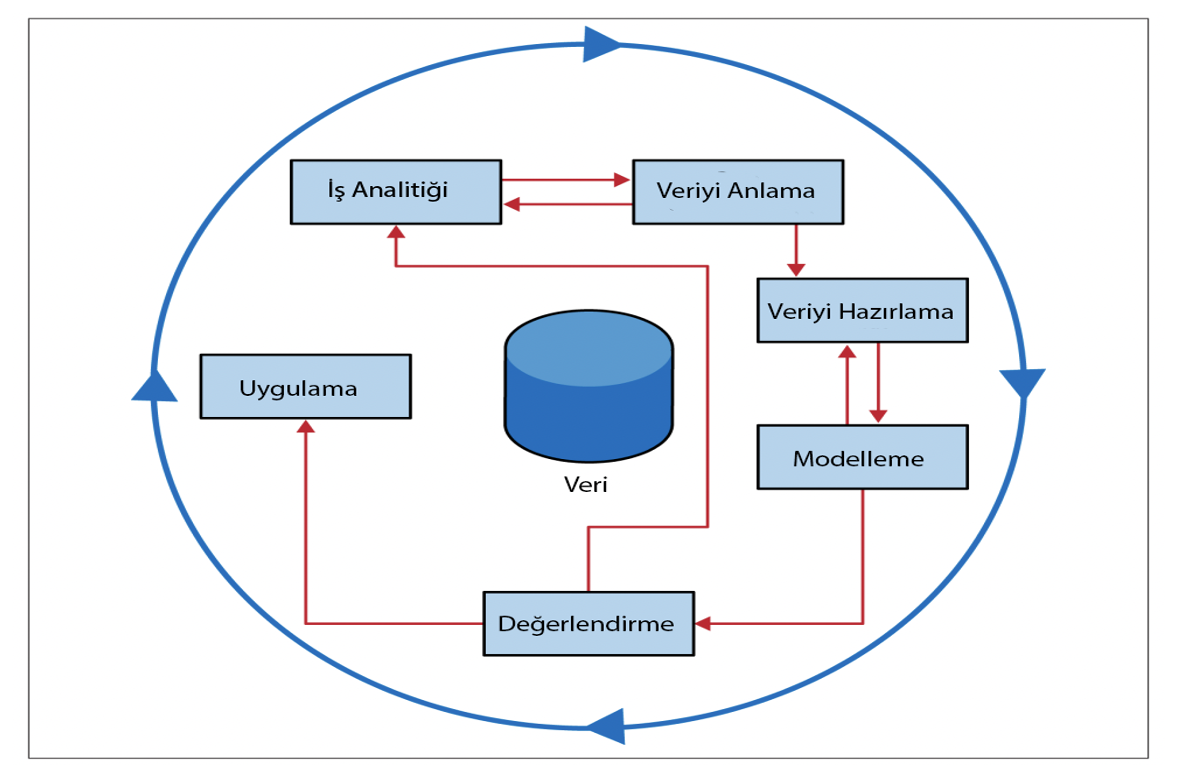
\includegraphics[width=0.95\linewidth,height=0.95\textheight]{tablolar-sekiller/sekil-4-1} \caption{Kaynak: (Mavimbela ve diğerleri, 2018: 42)}\label{fig:unnamed-chunk-1}
\end{figure}

Kaynak: (Provost ve Fawcett, 2013: 27)

Problemi anlama: Problemin tanımlanması, başlangıçta çözülmesi gereken sorunu anlamak için çok önemlidir. Bu açıkça görülebilir, ancak iş projeleri nadiren açık ve net veri madenciliği sorunları olarak ve önceden paketlenmiş olarak gelmektedir.
Veriyi anlama: Amaç, iş problemini çözmekse veriler çözümün oluşturulacağı mevcut ham maddeleri içerir. Verilerin güçlü yanlarını ve sınırlamalarını anlamak önemlidir. Çünkü nadiren problemle tam bir eşleşme nadiren vardır. Geçmiş veriler, genellikle mevcut iş sorunuyla ilgili olmayan amaçlar için veya hiçbir açık amaç olmaksızın toplanır. Bir müşteri veri tabanı, bir işlem veri tabanı ve bir pazarlama yanıtı veri tabanı farklı bilgiler içerir, kesişen farklı popülasyonları kapsayabilir ve değişen derecelerde güvenilirliğe sahip olabilir (Provost ve Fawcett, 2013).

Veriyi hazırlama: Genellikle verilerin manipüle edildiği ve daha iyi sonuçlar veren formlara dönüştürüldüğü veriyi anlamayla beraber veriyi hazırlama aşamasını ifade etmektedir. Örnek olarak; eksik değerleri çıkartmak ya da eksik veriye ortalama değer atmak, verileri farklı veri formatına çevirmek, veride aykırı değerler varsa bunların çıkartılması ya da normalleştirilmesi, ölçeklendirilmesi gibi birçok veri hazırlama tekniği bulunmaktadır.

\textbf{Modelleme:} Modelleme çıktısının bir tür model veya verideki düzenlilikleri yakalayan örüntüsü olarak tanımlanabilir. Tanımlanan problemin hedeflerinin gerçekleştirilmesi ve bundan istenilen sonuçların çıktısının sağlanması için araştırmada doğru algoritmanın kullanılması büyük önem arz etmektedir.
Değerlendirme: Değerlendirme aşamasının amacı, veri madenciliği sonuçlarını titizlikle değerlendirebilmekle beraber araştırmaya, geçerli ve güvenilir biçimde devam edildiğinden emin olmaktır.

Araştırmada yukarıda tanımlanan tüm aşamalar uygulanmıştır. Problemi tanımlama öncesinde, birçok farklı hesaptan (aktörden -- üniversiteler vb.) yarı yapılandırılmış veri setleri sağlanmıştır. Bu veri setleriyle ve araştırmanın amacı doğrultusunda, iklim aktörleri sınırlandırılmıştır. Çalışmanın teorik alt yapısına uygun bir şekilde, verilerden özellik çıkartımı işlemleri yapılmıştır. Örneğin, çalışmanın teorik bağlamında araştırılan diyalojik iletişim için linklerden kendi web sitesi paylaşımı, sosyal medya paylaşımı sınıflandırmaları yapılmıştır. Bu aşamada bazı problemlerle karşılanmıştır. Linklerin birçoğu; Bitly: URL'leri formatında yer almaktaydı. Bunun için ayrı bir algoritma yazılmıştır. Bu algoritma sayesinde, veri seti içerisinde yer alan tüm gözlemlerin linkleri taratılarak gerçek sayfa linklerine ulaşılmıştır.

\hypertarget{uxe7evre-ve-iklim-konu-modellemesi}{%
\subsubsection{Çevre ve İklim Konu Modellemesi}\label{uxe7evre-ve-iklim-konu-modellemesi}}

Otomatik İçerik Analizi (ACA), medya içeriğini otomatik olarak analiz etmek için kullanılan bir teknikler kombinasyonlarını ifade etmektedir. Eylemler ve iletişimler; teknolojik, bilişim sistemlerinin ilerlemesi sonucunda çevrimiçi ortamda daha sıklıkla gerçekleşmektedir, böylece dijital formatta kayıt halinde ve sayıca fazla olduğu göz önüne alınırsa, bu büyük miktardaki veriyi otomatik bir şekilde analiz etmek bir zorunluluk halini almıştır. Hesaplamalı Sosyal Bilimler çerçevesinde yer alan, sözlük ve kelime frekansı tabanlı yöntemlerde; doğal dil işleme, denetimli ve denetimsiz makine öğrenimi dahil olmak üzere bilgisayar bilimi ve hesaplamalı dilbilim gibi disiplinlerin tekniklerinden yararlanılmaktadır (Digicomlab , 2022).

\textbf{Şekil 4.2:} Veri Yöntemleri Olarak Metne Genel Bakış.

\begin{figure}
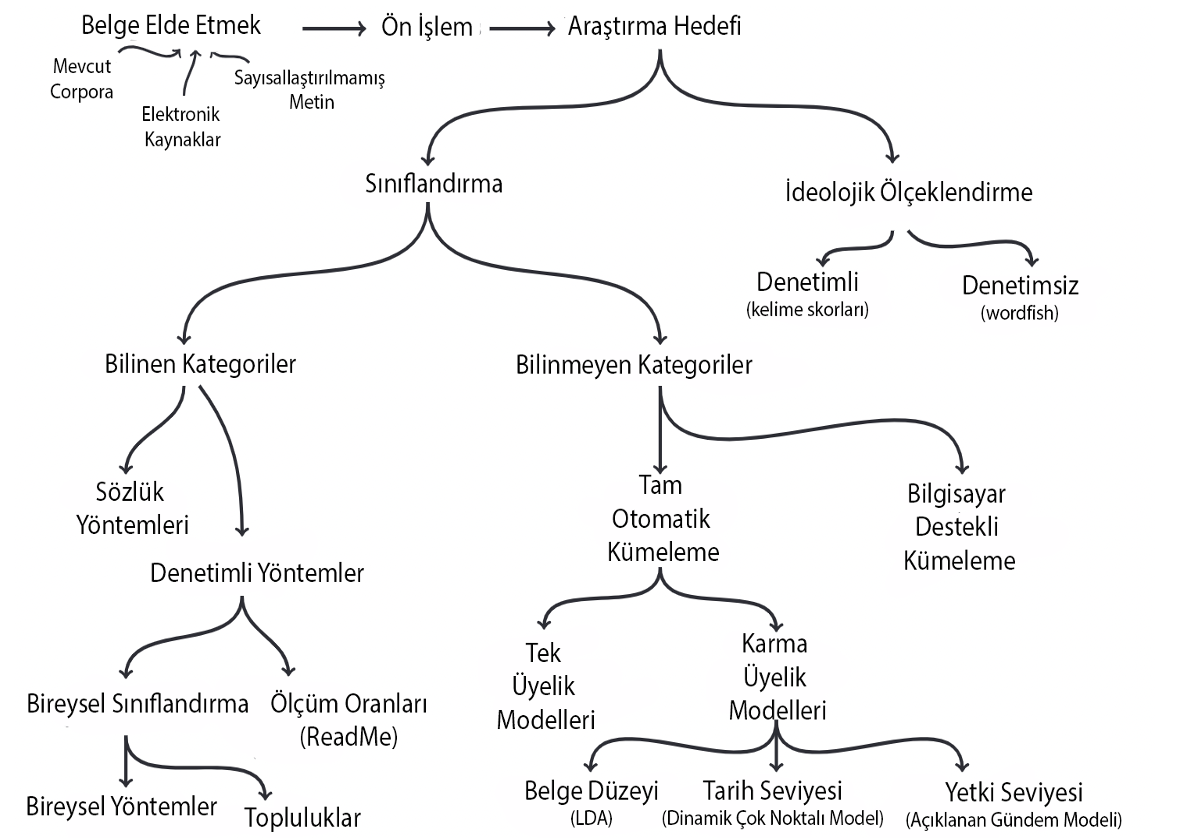
\includegraphics[width=0.95\linewidth,height=0.95\textheight]{tablolar-sekiller/sekil-4-2} \caption{Kaynak: (Grimmer ve Stewart, 2013: 268)}\label{fig:unnamed-chunk-2}
\end{figure}

Kaynak: (Grimmer ve Stewart, 2013: 268)

``Introduction to Machine Learning'' kitabında gözetimli ve gözetimsiz öğrenme aşağıdaki gibi tanımlanmaktır (Alpaydın, 2014).

Gözetimli Öğrenme (Supervised Learning-Classification): Gözetimli öğrenme ya da denetimli öğrenme olarak adlandırılan bu öğrenme yaklaşımında amaç, doğru değerlerin bir süpervizör tarafından sağlanan girdiden çıktıya kadar bir eşleme öğrenmektir.
Gözetimsiz Öğrenme (Unsupervised Learning-Clustering): Gözetimsiz ya da denetimsiz öğrenmede gözetimli öğrenmedeki gibi bir süpervizör bulunmamaktadır. Elimizde sadece girdi verisi bulunur. Amaç girdi düzenliliklerini bulmaktır. Girdi uzayının belirli kalıplarında diğerlerinden daha sık meydana gelen bir yapı bulunmaktadır. Genellikle neyin olup neyin olmadığı görülmek istenir. İstatistikte buna yoğunluk tahmini denir.
Çalışmanın iklim konularını sınıflandırmaya yönelik yapılan makine öğrenmesi araştırmasında bilinmeyen kategoriler için olan tam otomatik kümelemeyi ifade eden denetimsiz öğrenme yöntemi kullanılmıştır. Denetimsiz öğrenmede, küme sayısını ifade eden k (k-means) değeri 20 olarak belirlenmiştir. Veri setindeki içerikler, belirlenen 20 adet kümede gruplanmıştır. Literatür bilgisiyle benzer başlıklar ve iç içe geçen temalar tek başlık altında toplanmıştır. Sonuç olarak, 9 farklı kategori belirlenmiştir.

Metinler denetimsiz öğrenme yöntemi kullanılarak ilk önce 20 kümede sınıflandırılmıştır. Bunun için RStudio programı ve quanteda kütüphanesi (Topic models) kullanılarak LDA konu modellemesi kullanılmıştır. Latent Dirichlet Allocation, doğal dil işlemede (NLP -- Natural Language Processing) kullanılan her bir belgenin bir konu koleksiyonu kabul edilmesi ve belgedeki her kelimenin konulardan birine karşılık gelmesi mantığı ile çalışmaktadır. Bu, belgelerin doğal dilin tipik kullanımını yansıtacak şekilde; ayrı gruplara ayrılmak yerine, içerik açısından birbirleriyle ``örtüşmesine'' olanak tanımaktadır (Silge ve Robinson, 2018). Yapılan denetimsiz öğrenme çıktılarına göre benzer sonuçlar / anlamlar çıkan kümeler birleştirilerek 9 adet sınıfa kadar indirgenmiştir.

LDA yönetimi ile yapılan iklim çalışmalardan bir tanesi de Boussalis ve Goan'nın ``Text-mining the signals of the climate doubt'' araştırmasıdır. Bu araştırmada 1998-2013 yıllarını kapsayan 19 organizasyondan elde edilen 16000 doküman taranmıştır. Araştırmanın sonucuna göre, iklim tartışmaları bu zaman aralığında artış göstermiştir (Boussalis ve Coan, 2016).

İklim iletişimi zorlukları başlığında değinilen mesajların karmaşıklığı, verilerin kümelenmesi sürecinde de ortaya çıkmıştır. Tema çeşitliliğinin fazlalığı ve konuların birbirleriyle iç içe geçmiş olması sınıflandırma sürecinde güçlükler meydana getirmiştir.

\textbf{Tablo 4.1:} Çevre ve İklim Temaları.

\begin{figure}
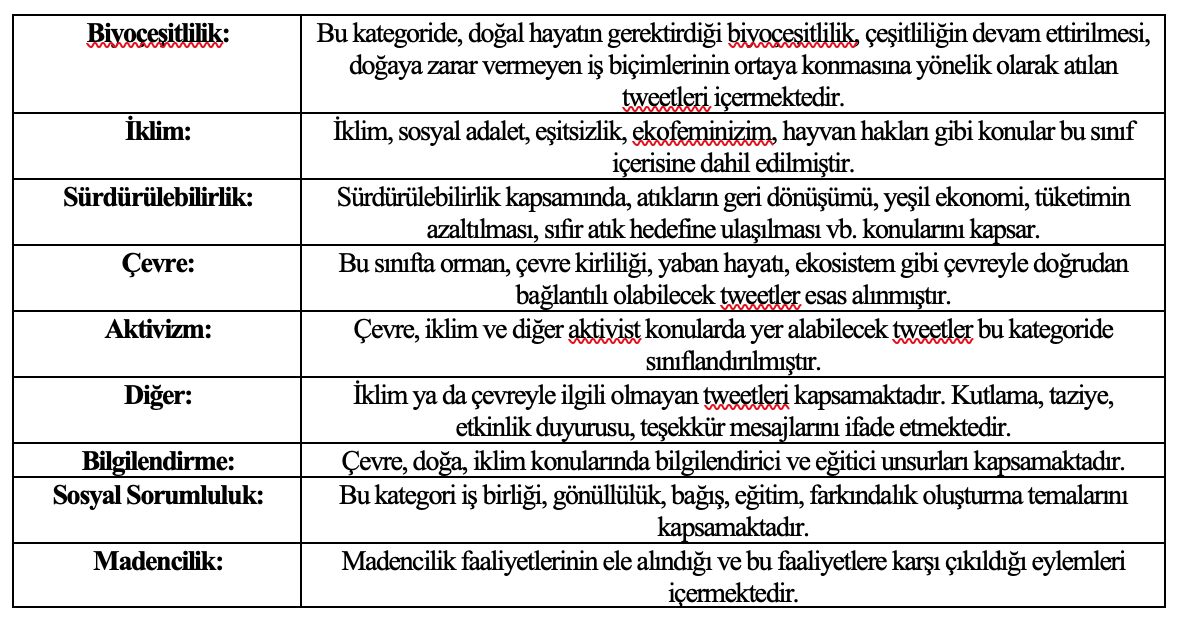
\includegraphics[width=0.95\linewidth,height=0.95\textheight]{tablolar-sekiller/tablo-4-1} \caption{Kaynak: (Mavimbela ve diğerleri, 2018: 42)}\label{fig:unnamed-chunk-3}
\end{figure}

Biyoçeşitlilik: Bu kategoride, doğal hayatın gerektirdiği biyoçeşitlilik, çeşitliliğin devam ettirilmesi, doğaya zarar vermeyen iş biçimlerinin ortaya konmasına yönelik olarak atılan tweetleri içermektedir.

İklim: İklim, sosyal adalet, eşitsizlik, ekofeminizim, hayvan hakları gibi konular bu sınıf içerisine dahil edilmiştir.

Sürdürülebilirlik:
Sürdürülebilirlik kapsamında, atıkların geri dönüşümü, yeşil ekonomi, tüketimin azaltılması, sıfır atık hedefine ulaşılması vb. konularını kapsar.
Çevre: Bu sınıfta orman, çevre kirliliği, yaban hayatı, ekosistem gibi çevreyle doğrudan bağlantılı olabilecek tweetler esas alınmıştır.
Aktivizm: Çevre, iklim ve diğer aktivist konularda yer alabilecek tweetler bu kategoride sınıflandırılmıştır.
Diğer: İklim ya da çevreyle ilgili olmayan tweetleri kapsamaktadır. Kutlama, taziye, etkinlik duyurusu, teşekkür mesajlarını ifade etmektedir.
Bilgilendirme: Çevre, doğa, iklim konularında bilgilendirici ve eğitici unsurları kapsamaktadır.
Sosyal Sorumluluk: Bu kategori iş birliği, gönüllülük, bağış, eğitim, farkındalık oluşturma temalarını kapsamaktadır.
Madencilik: Madencilik faaliyetlerinin ele alındığı ve bu faaliyetlere karşı çıkıldığı eylemleri içermektedir.

\hypertarget{evren-ve-uxf6rneklem}{%
\subsection{Evren ve Örneklem}\label{evren-ve-uxf6rneklem}}

Twitter kuruluşların, hükümetlerin ve siyasi kampanyaların faaliyetlerinde giderek daha önemli bir rol oynamaktadır (Sundstrom ve Levenshus, 2017). Kişiler ve kuruluşlar için Twitter, ulusal ve uluslararası etkinlikler hakkında gerçek zamanlı bilgiler sunmaktadır. Araştırmanın veri kaynağı, sosyal ağ uygulaması Twitter'dan elde edilmiştir.

Twitter üç nedenden dolayı tercih edilmiştir (Wang \& Yang, 2020: 10).
1) Küresel şirketler tarafından en yaygın kullanılan sosyal medya kanalı olması.
2) Diyalojik iletişim için mention, hashtag, media, linkler gibi birçok faydalı özellik sunması.
3) Hemen hemen tüm kurumların Twitter sayfalarına herhangi bir kullanıcı tarafından erişilebilir olmasıdır.

Aktörler, iklim aktörleri konusunda daha önce yapılmış çalışmalardan yola çıkılarak belirlenmiştir (Özer, 2017; Özmen, 2011; Ü. Şahin, 2014). Politikaların yürütülmesi, izlenmesi, denetlenmesi, geliştirilmesi görevleri olan bakanlıklarla (Yağmurlu, 2019); ve toplumsal çıkarları ve hakları koruma, sosyal, toplumsal ve çevresel konularda bireyleri eğitme, bilinçlendirme misyonu olan sivil toplum kuruluşları; araştırma örnekleminin iki ana aktörüdür. Araştırmada, 5 sivil toplum kuruluşu ve 5 bakanlık olmak üzere on farklı aktör yer almaktadır. Araştırma 01.01.2020 ile 01.01.2022 tarihleri arasındaki iki senelik zaman aralığını kapsamaktadır. İklim aktörlerinin bu iki yıllık zaman periyodundaki tüm tweetleri, çalışmanın örneklemini oluşturmaktadır.

\hypertarget{verilerin-toplanmasux131-ve-analizi}{%
\subsection{Verilerin Toplanması ve Analizi}\label{verilerin-toplanmasux131-ve-analizi}}

Verilerin toplanması süreci Python ve Twitter API aracılığıyla gerçekleştirilmiştir. Analizler ve diğer uygulamalar için Python, RStudio, Google Spreadsheet, Excel programları birlikte kullanılmıştır. Tüm aktörler için veri çekme işlemi ayrı ayrı gerçekleşmiştir. Veri çekme işlemi iki senelik zaman aralığını kapsamaktadır. Araştırma kapsamında 01/01/2020 -- 01/01/2022 tarihleri arasındaki ilgili aktörlerin tüm tweetleri toplanmıştır. Toplam gözlem sayısı N = 17381'tir. Araştırma tasarımı oluşturulana kadarki süreçte, çalışılan veri sayısı 110513'tür. Tasarım oluşturma süreçlerinde belediye, iş dünyası, üniversiteler dahil olmak üzere farklı aktörlerden veriler çekilerek onların içerikleri incelenmiştir. İnceleme sonucunda; bakanlıklar ve sivil toplum kuruluşları, karşılaştırma bakımından en uygun iklim aktörleri olarak belirlenmiştir.

n\_stk:9617+ n\_bakanliklar: 7764 = 17381

\textbf{Şekil 4.3:} Sivil Toplum Kuruluşları Tweet Sayısı 2020-2021.

\begin{figure}
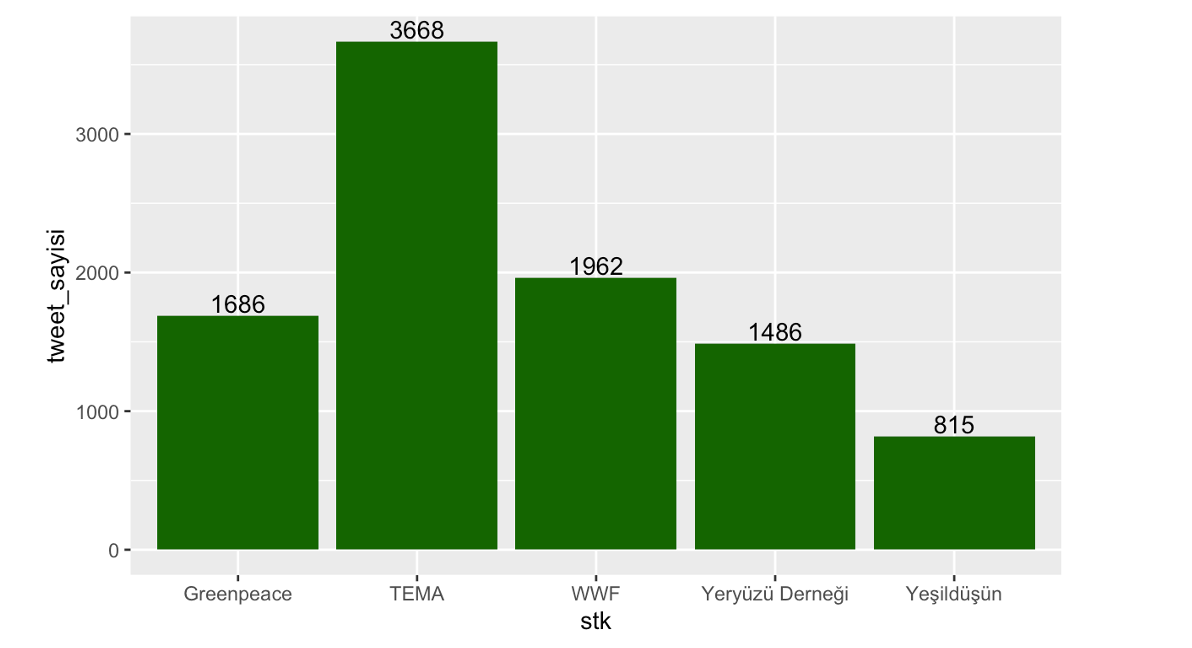
\includegraphics[width=0.95\linewidth,height=0.95\textheight]{tablolar-sekiller/sekil-4-3} \caption{Kaynak: (Mavimbela ve diğerleri, 2018: 42)}\label{fig:unnamed-chunk-4}
\end{figure}

\textbf{Şekil 4.4:} Bakanlıklar Tweet Sayısı 2020-2021.

\begin{figure}
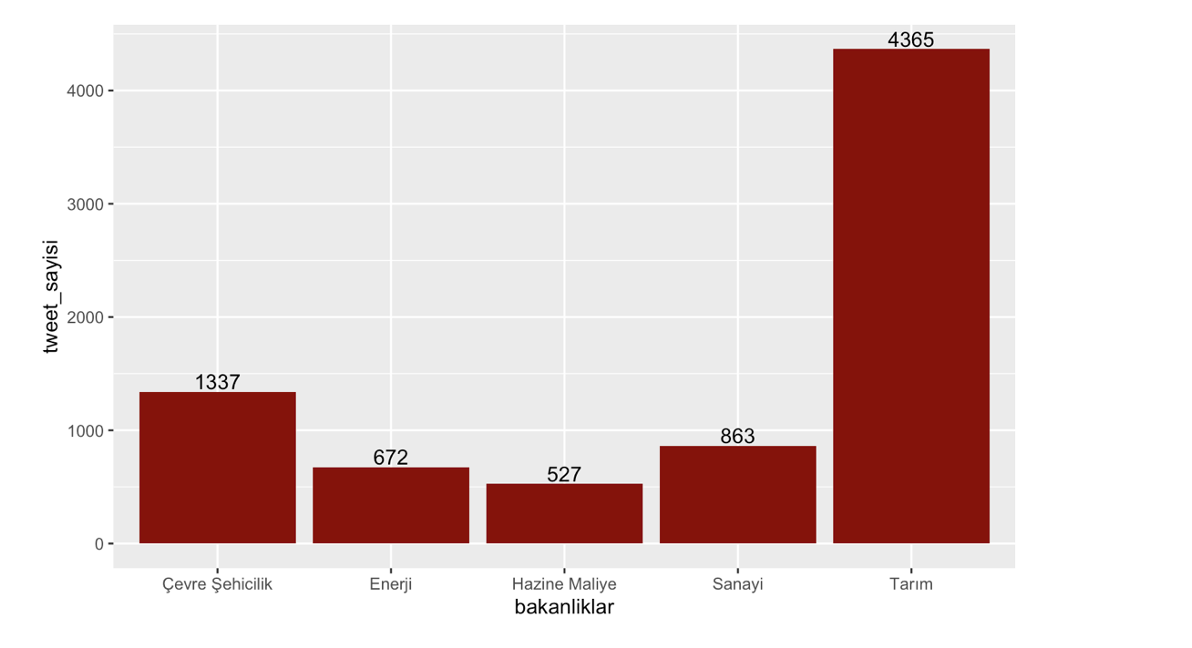
\includegraphics[width=0.95\linewidth,height=0.95\textheight]{tablolar-sekiller/sekil-4-4} \caption{Kaynak: (Mavimbela ve diğerleri, 2018: 42)}\label{fig:unnamed-chunk-5}
\end{figure}

\textbf{Tablo 4.2:} Bakanlıklar ve STK'ların Toplam Tweet Sayısı Betimsel İstatistikleri.

\begin{figure}
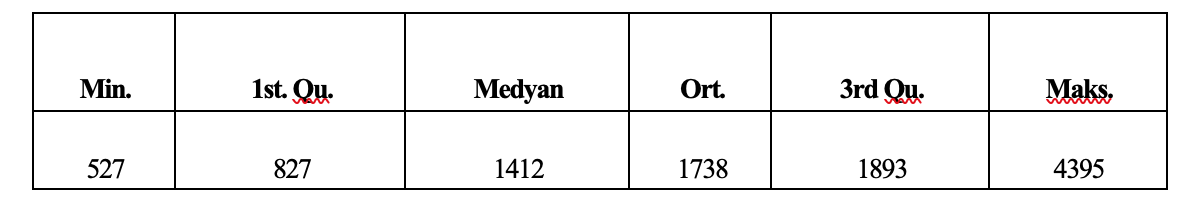
\includegraphics[width=0.95\linewidth,height=0.95\textheight]{tablolar-sekiller/tablo-4-2} \caption{Kaynak: (Mavimbela ve diğerleri, 2018: 42)}\label{fig:unnamed-chunk-6}
\end{figure}

\hypertarget{bulgular}{%
\section{Bulgular}\label{bulgular}}

Bu başlıkta, araştırmanın bulguları yorumlanmakta ve araştırma sorularına cevaplar aranmaktadır. Çalışma kapsamında; (1) diyalojik iletişim, (2) dört-model ve (3) çevre ve iklim konu modellemesi olmak üzere üç farklı araştırmanın bulguları ortaya koyulmaktadır.

\hypertarget{diyalojik-iletiux15fim}{%
\subsection{Diyalojik İletişim}\label{diyalojik-iletiux15fim}}

\textbf{AS1:} İklim aktörleri Twitter sayfalarında diyalojik ilkeleri nasıl kullanmaktadır?
\textbf{AS2:} İklim aktörlerinin diyalojik ilkeleri, Twitter'da uygulamaları açısından bir farklılık gösteriyor mu?

Sivil toplum kuruluşları ve bakanlıklar, 2020-2021 zaman aralığında toplam 17381 tweet atmışlardır. Sivil toplum kuruluşlarının 9617 tweet attığı gözlemlenmiştir. STK'ların tweetlerinin toplam tweetlere oranı \%57,65'tir. Bakanlıklar 7764 tweet atmıştır, bunun toplam tweetlere oranı \%42,35'tir.

İlk araştırma soruları AS1 ve AS2, bakanlıklar ile sivil toplum kuruluşlarının Twitter sayfalarındaki diyalojik ilkeleri uygulama biçimlerinin farklılığına odaklanmaktadır.
Bilginin kullanışlılığı ilkesine göre; kurumlarca en sık kullanılan bilgi paylaşım biçimlerinin fotoğraflar olduğu tespit edilmiştir (\%51,77, n\_fotoğraf = 9492). İkinci sırada ise daha çok metin formatında içerikler (\%33,88, n\_metin = 6212) paylaştıkları gözlemlenmiştir. En az frekansta paylaşım yapılan içerik türünün ise videolar (\%9,15, n\_video = 1677) olduğu saptanmıştır. Ayrıca ki-kare testi STK'lar ve bakanlıkların fotoğraf (p \textless{} .001), metin (p \textless{} .001), video (p \textless{} .001), kullanımları arasında istatistiksel olarak önemli farklılıklar olduğunu göstermektedir. Daha spesifik olarak, aşağıda Tablo 4.3'de gösterildiği gibi, sivil toplum kuruluşları paylaşımlarında; metin (\%41,44, n\_metin = 3985) ve (\%53,99, n\_fotoğraf = 5192) fotoğraf formatlarını içerik olarak bakanlıklara göre daha fazla kullanmışlardır. Video paylaşımlarında ise bakanlıklar (\%15,93, n\_video = 1237) STK'lardan (\%4,58, n\_video = 440) önemli ölçüde daha fazla içerik paylaşmışlardır.

Ziyaretçilerin elde tutulması ilkesi, tüm kuruluşların tweetlerinin \%14,73'ü (n\_kendiwebsitepaylaşımı = 2700) oranında kendi web sayfalarına bağlantılar içermektedir. Ki-kare testi bakanlıkların (\%17,90, n\_kendiwebsitepaylaşımı = 1390), ve STK'ların (\%13,62, n\_kendiwebsitepaylaşımı = 1310), kendi websitesi paylaşımlarında (χ2(1, n\_kendiwebsitepaylaşımı = 2700) = 1009.8, р \textless{} .001) önemli ölçüde farklılaştığını göstermektedir. Sosyal medya paylaşımları ise toplam tweetlerin \%5,05 oluşturmaktadır. Yapılan ki-kare (χ2(1, n\_(sosyal-ağ-paylaşımı) = 926) = 8.5371, р \textgreater{} .001) testi sonucunda bakanlıklar ve STK'ların sosyal medya paylaşımları arasında anlamlı bir farklılık olmadığını görülmektedir.

Yeniden Ziyaretçi Sağlama ilkesi; toplam tweetlerin \%76,80'de (n\_(ek-bilgiler) = 14081) ek bilgilerin alınabileceği web sitelerine bağlantılar yer almaktadır. STK'lar (\%83,48, (n\_(ek-bilgiler)= 8028) önemli ölçüde bakanlıklara (\%77,96 n\_(ek-bilgiler)= 6053) göre daha fazla ek bilgilerin yer aldığı web sitesi bağlantısı paylaşımı yaptığı tespit edilmiştir (χ2(1, n\_(ekbilgi-sayfaları) = 14081) = 2429.7, р \textless{} .001).
Diyalojik döngü ilkesi tüm kuruluşların \%4,07'i kullanıcı tweetlerine cevap vermiştir. Ki-kare testi, STK'lar (\%3,97, n\_cevaplama= 382) bakanlıklara (\%4,69, n\_cevaplama= 364) göre (χ2(1, n\_cevaplama = 746) = 225.25, р \textless{} .001) istatistiksel olarak manidar ölçüde daha fazla kullanıcılara yanıt verdiğini göstermektedir. Kuruluşlar tweetlerin \%16,59'da kullanıcı etiketlemişlerdir. Yapılan ki-kare testinde STK'lar (〖\%13,40,n〗\_etiketleme=1289) ve bakanlıklar (\%22,58, n\_etiketleme = 1753) kullanıcıların etiketlenmesi açısından manidar bir farklılığın olduğu ortaya çıkarmıştır (χ2(1, n\_etiketleme = 3042) = 1727, р \textless{} .001). Bir diğer diyalojik döngü indeksi olan hashtag kullanımında; kuruluşlar tweetlerin \%37,56'da (n\_hashtag=6887) hashtag kullanmıştır. Ki-kare testi neticesinde STK'lar (\%40,66, n\_hashtag = 3910) bakanlıklardan (〖\%38,34,n〗\_hashtag = 2977) önemli ölçüde daha fazla hashtag kullandığı tespit edilmiştir (χ2(1, n\_hashtag = 6887) = 1220.2, р \textless{} .001).

\textbf{Tablo 4.3:} Diyalojik İletişim Prensiplerinin Frekansı.

\begin{figure}
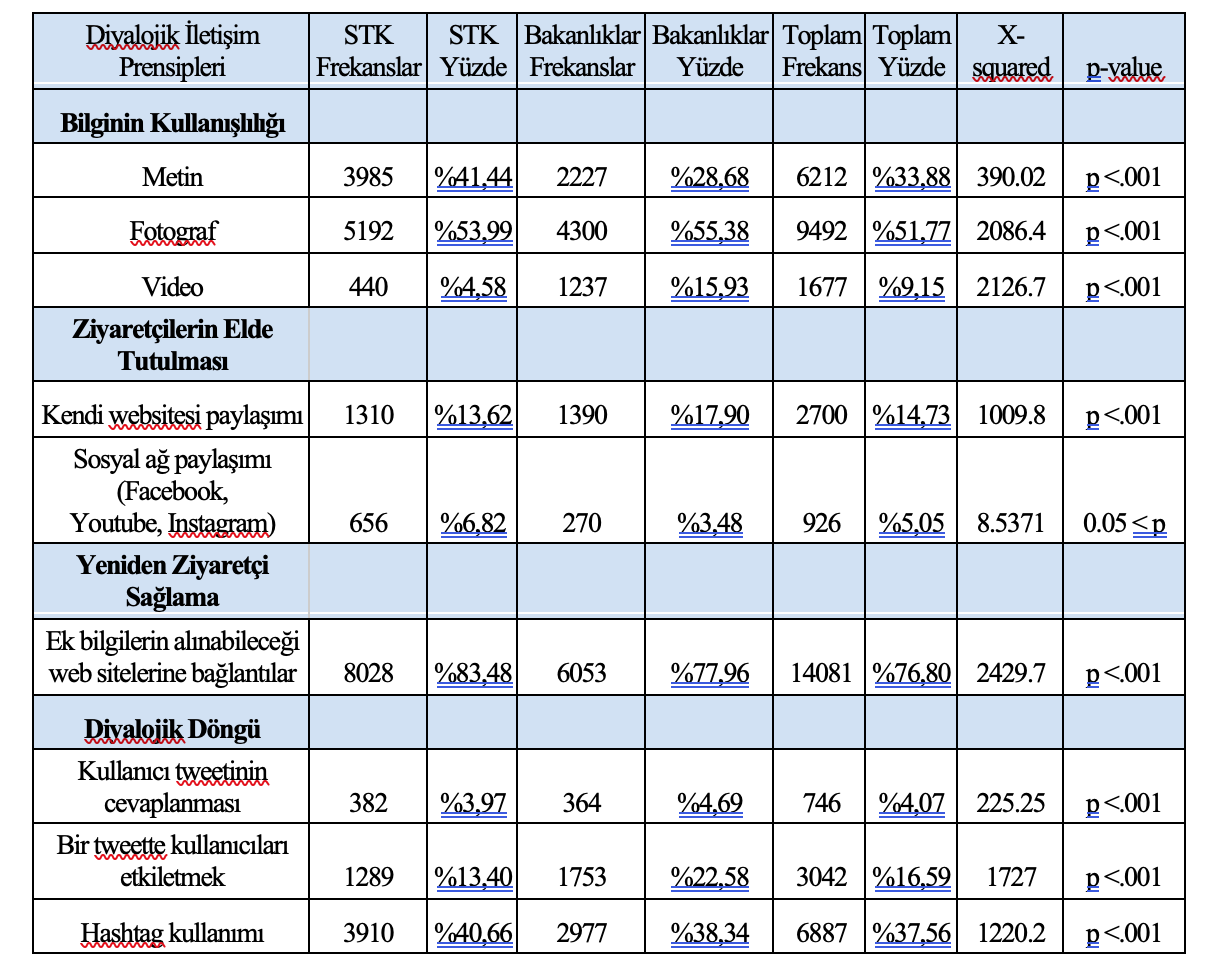
\includegraphics[width=0.95\linewidth,height=0.95\textheight]{tablolar-sekiller/tablo-4-3} \caption{Kaynak: (Mavimbela ve diğerleri, 2018: 42)}\label{fig:unnamed-chunk-7}
\end{figure}

\textbf{AS3:} Hedef kitleler beğeniler, retweetler ve yorumlar açısından Twitter'daki aktörlerle nasıl etkileşime girmektedir?

\textbf{AS4:} İklim aktörleri arasında beğeniler, retweetler ve yorumlar açısından kamu katılımında bir fark var mı?

Araştırmada kitlelerin Twitter'daki kuruluşlarla beğenileri, retweetleri ve yorumlarından yola çıkarak etkileşim kurma biçimleri incelenmiştir. Kuruluşların retweet sayıları: 0 ile 31864 arasında, ortalaması 25 (SD = 509), beğeni sayıları: 0 ile 82816 arasında, ortalaması 281 (SD = 1413), yorum sayıları: 0 ile 8596 arasında, ortalaması 21 (SD = 156) olarak tespit edilmiştir. Yapılan normallik testi; beğeni, retweet ve yorum verilerinin normal bir dağılım izlemediğini göstermektedir. Literatürde normallik testinin yapılabilmesi için örneklem değerinin N \textless{} 5000'den küçük olması gerektiği belirtilmektedir. Büyük veri setlerinde normallik varsayımlarının yapılmasının gereksizliğini vurgulayan görüşler de bulunmaktadır (Cross Validated). Bu sebepten dolayı, veri setinden rastsal olarak 2000 örneklem seçilmiştir. Aykırı değerler çıkartılarak tekrar normallik testleri uygulanmıştır. Yine de veri setinin normal dağılımı sağlamadığı tespit edilmiştir.

\textbf{Tablo 4.4:} Beğeni, Retweet ve Yorum Sayısı Betimsel İstatistikler.

\begin{figure}
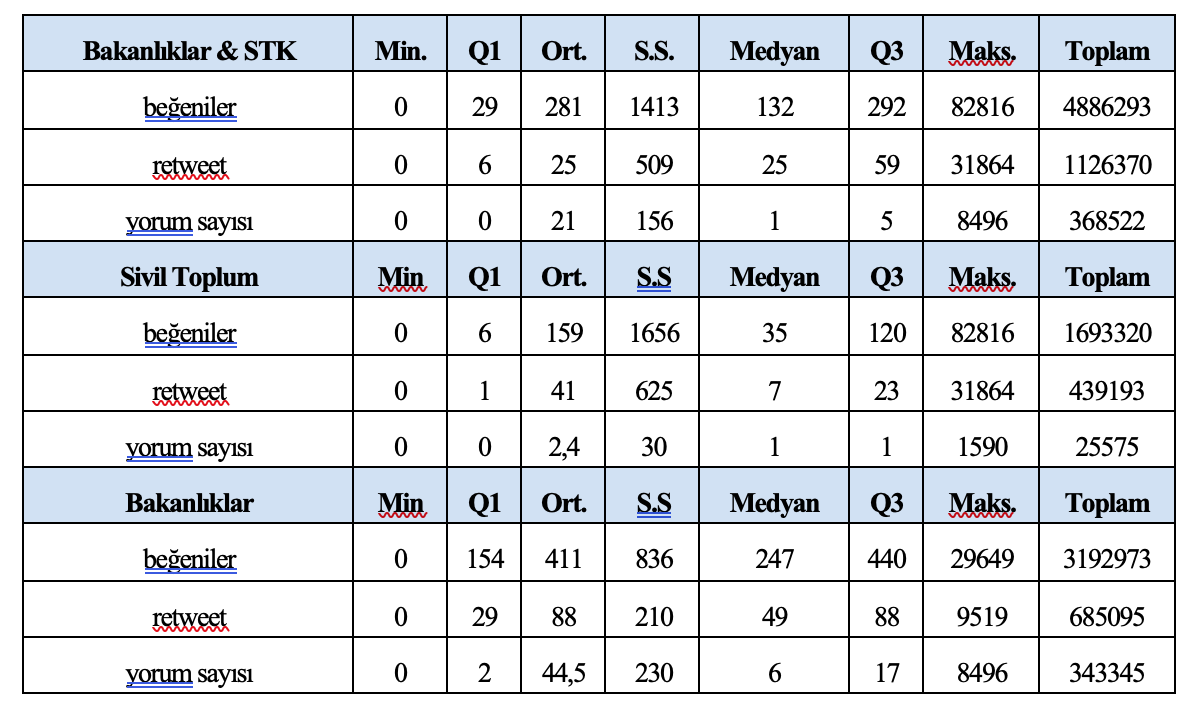
\includegraphics[width=0.95\linewidth,height=0.95\textheight]{tablolar-sekiller/tablo-4-4} \caption{Kaynak: (Mavimbela ve diğerleri, 2018: 42)}\label{fig:unnamed-chunk-8}
\end{figure}

Araştırma; kuruluşların diyalojik iletişiminin halkın katılımı üzerindeki etkisine de odaklandı. Her diyalojik ilke indeksi için beğeni, retweet ve yorum ortalamaları; aşağıda Tablo 4.5'de gösterilmektedir. Yapılan Kruskal Wallis testi sonuçları; metin {[}H(1, 6212)= 3740.7, p\textless.001{]}, fotoğraf {[}H(1, 9492)= 5394.7, p\textless.001{]}, video {[}H(1, 1677)= 625.0, p\textless.001{]}, kurumların kendi web sitesi paylaşımları {[}H(1, 2700)= 1708.9, p\textless.001{]}, sosyal ağ paylaşımları {[}H(1, 926)= 520.3, p\textless.001{]}, ek bilgilerin alınabileceği web sitelerine bağlantıları {[}H(1, 14081)= 7344.5, p\textless.001), kullanıcı tweetlerinin cevaplanması {[}H(1, 746)= 44.9, p\textless.001{]}, bir tweette kullanıcıların etiketlenmesi {[}H(1, 3042)= 1368.0, p\textless.001{]}, hashtag kullanımı {[}H(1, 6887)= 3666.9, p\textless.001{]} ve beğeni sayıları arasında güçlü bir ilişki olduğunu göstermektedir. Retweetler için yapılan Kruskal Wallis testi sonuçları da; metin {[}H(1, 6212)= 3118.8, p\textless.001{]}, fotoğraf {[}H(1, 9492)= 4625.2, p\textless.001{]}, video {[}H(1, 1677)= 413.4, p\textless.001{]}, kurumların kendi web sitesi paylaşımları {[}H(1, 2700)= 1414.5, p\textless.001{]}, sosyal ağ paylaşımları {[}H(1, 926)= 406.2, p\textless.001{]}, ek bilgilerin alınabileceği web sitelerine bağlantıları {[}H(1, 14081)= 6211.1, p\textless.001), kullanıcı tweetlerinin cevaplanması {[}H(1, 746)= 68.8, p\textless.001{]}, bir tweette kullanıcıların etiketlenmesi {[}H(1, 3042)= 1106.6, p\textless.001{]}, hashtag kullanımı {[}H(1, 6887)= 3061.9, p\textless.001{]} ve retweet sayıları arasında güçlü bir ilişki olduğunu göstermektedir. Ek olarak, yorum sayısı ile metin {[}H(1, 6212)= 2599.6, p\textless.001{]}, fotoğraf {[}H(1, 9492)= 4596.0, p\textless.001{]}, video {[}H(1, 1677)= 608.9, p\textless.001{]}, kurumların kendi web sitesi paylaşımları {[}H(1, 2700)= 1559.1, p\textless.001{]}, sosyal ağ paylaşımları {[}H(1, 926)= 491.8, p\textless.001{]}, ek bilgilerin alınabileceği web sitelerine bağlantıları {[}H(1, 14081)= 6178.3, p\textless.001), kullanıcı tweetlerinin cevaplanması {[}H(1, 746)= 69.7, p\textless.001{]}, bir tweette kullanıcıların etiketlenmesi {[}H(1, 3042)= 785.5, p\textless.001{]}, hashtag kullanımı {[}H(1, 6887)= 2192.8, p\textless.001{]} arasında güçlü bir ilişki olduğunu göstermektedir.

\textbf{Tablo 4.5:} Diyalojik İletişim Kullanıcı Etkileşimi Test Sonuçları.

\begin{figure}
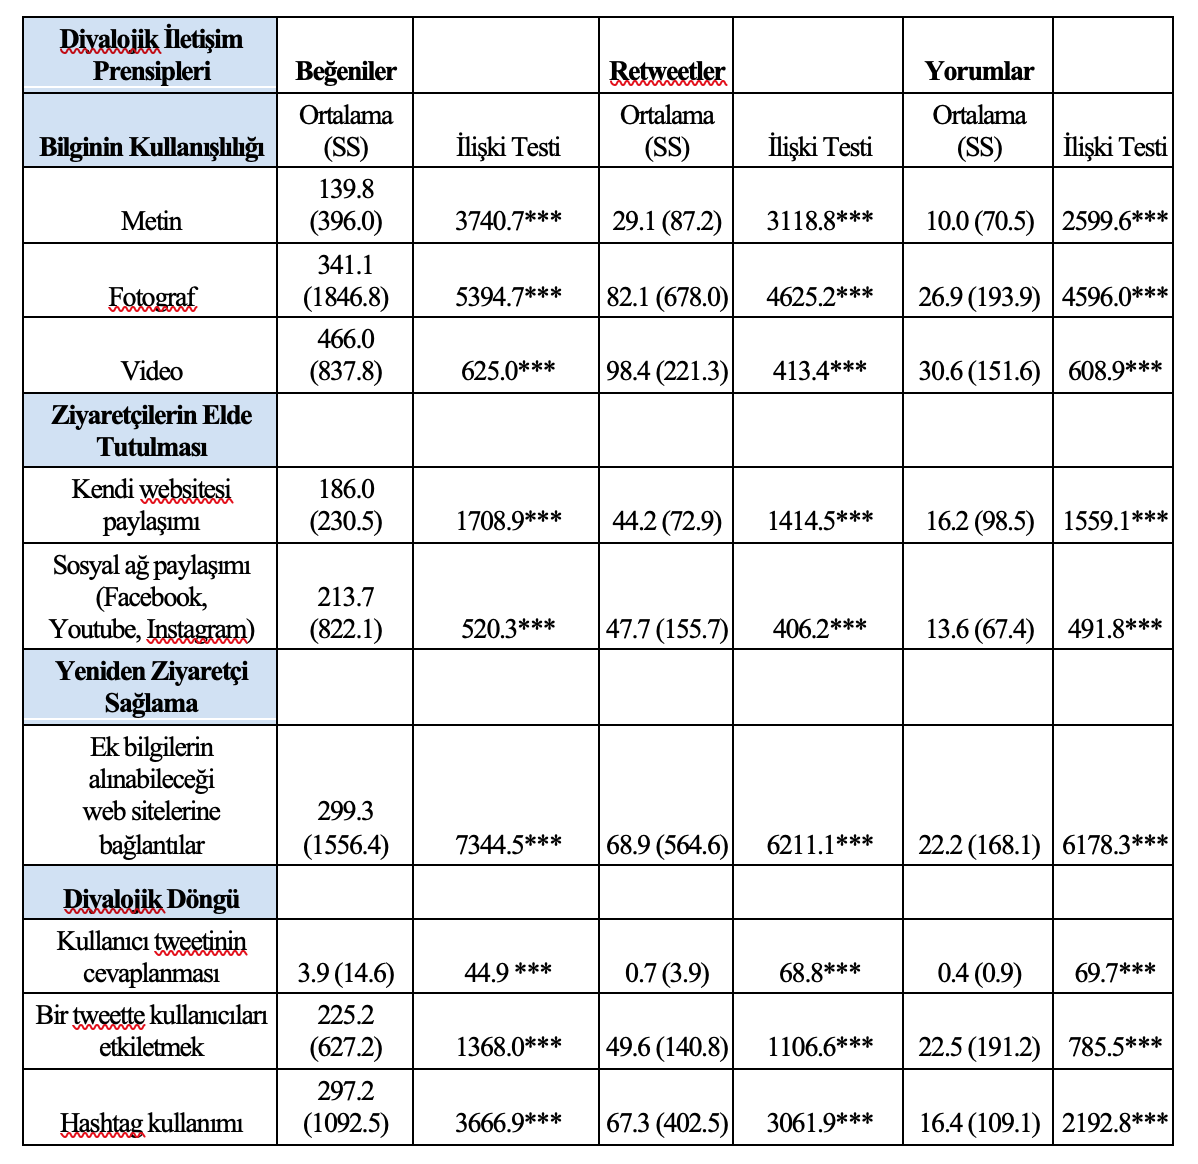
\includegraphics[width=0.95\linewidth,height=0.95\textheight]{tablolar-sekiller/tablo-4-5} \caption{Kaynak: (Mavimbela ve diğerleri, 2018: 42)}\label{fig:unnamed-chunk-9}
\end{figure}

\hypertarget{iklim-aktuxf6rleri-iletiux15fimlerinin-grunig-huntun-duxf6rt-modeli-baux11flamux131nda-deux11ferlendirilmesi}{%
\subsection{İklim Aktörleri İletişimlerinin Grunig -- Hunt'un Dört Modeli Bağlamında Değerlendirilmesi}\label{iklim-aktuxf6rleri-iletiux15fimlerinin-grunig-huntun-duxf6rt-modeli-baux11flamux131nda-deux11ferlendirilmesi}}

\textbf{AS5:} İklim aktörleri Twitter üzerindeki iletişimlerini Grunig ve Hunt'un dört modeline göre nasıl konumlandırmaktadır?

Grunig'in dört model yaklaşımı, temelde modelleri, onların tek yönlü mü yoksa iki yönlü mü, asimetrik mi yoksa simetrik mi olmalarına göre sınıflandırmaktadır. Bu kodlama kategorilerinin çoğu önceki sosyal medya araştırmalarından uyarlanmıştır (Grunig, 2009; Phillips-LeverWealth) ve teorik bağlama uyacak şekilde değiştirilmiştir. İçerik analizi, araçsal olarak değerlendirilmiştir. Araştırma sürecinde elde edilen veriler, Phillips ve Grunig'in tartışmış olduğu sınıflandırma ölçüsünde de değerlendirilmiştir. İçerikler, birden fazla halkla ilişkiler modeline dahil olabildiğinden dolayı aritmetik ortalama ile hesaplama işlemleri yapılmıştır. Phillips'in Dijital İletişim Araçları Modeli, araştırmanın birinci bölümünde anlatılmıştır. Bu kategorilendirme yaklaşımıyla frekanslar elde edilmiştir ve sonrasında ki-kare testi gerçekleştirilmiştir. Aşağıdaki tabloda Grunig'in dört modeli için belirlenen sınıflandırmalar yer almaktadır.

Dijital çağda, trendler hızla değişmektedir. Halkla ilişkiler uygulayıcıları sosyal medyayı bir halkla ilişkiler aracı olarak görmektedir. Halkla ilişkiler stratejik yönetim paradigması içinde yer alan etkileşim, stratejik iletişim, dört model gibi uygulamaların sosyal medyanın kendi özellikleri içerisinde yer alması, onun kullanımını cazip hale getirmektedir (James, E. Grunig, 2009).

\textbf{Tablo 4.6:} Grunig ve Hunt Dört Halkla İlişkiler Modeli.

\begin{figure}
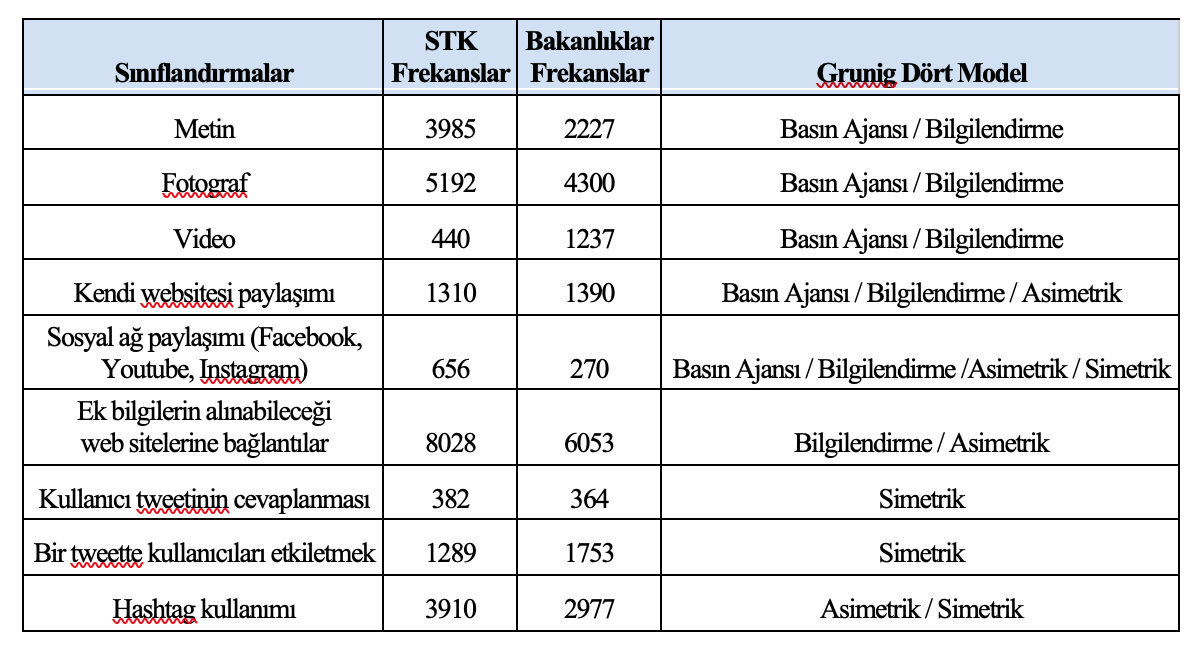
\includegraphics[width=0.95\linewidth,height=0.95\textheight]{tablolar-sekiller/tablo-4-6} \caption{Kaynak: (Mavimbela ve diğerleri, 2018: 42)}\label{fig:unnamed-chunk-10}
\end{figure}

Sivil toplum kuruluşları ve bakanlıkların Twitter kullanımları arasındaki ilişkiyi, Grunig ve Hunt'un dört halkla ilişkiler modeli açısından incelemek için ki-kare testi yapılmıştır (Tablo 4.7). Yapılan ki-kare testi sonucu; χ2(3, n\_(iklim-aktörleri) = 17381) = 70.338, р \textless{} .001 bakanlıklar ve STK'ların Twitter üzerindeki iletişimleri arasında, halkla ilişkiler modelleri açısından istatistiksel olarak anlamlı bir farklılık olduğunu ortaya çıkarmıştır. Her iki iklim aktörü grubunun da bilgilendirme modelini ağırlıklı olarak kullandığı tespit edilmiştir. Sivil toplum kuruluşlarının asimetrik ve simetrik modelleri bakanlıklardan daha fazla kullandığı ortaya çıkmıştır. Her iki aktör grubu için model kullanım sıralaması şu şekildedir.

Kamuoyu Bilgilendirme \textgreater{} Asimetrik \textgreater{} Basın Ajansı \textgreater{} Simetrik

\textbf{Tablo 4.7:} Grunig-Hunt Dört Halkla İlişkiler Modeli Çapraz Tablosu.

\begin{figure}
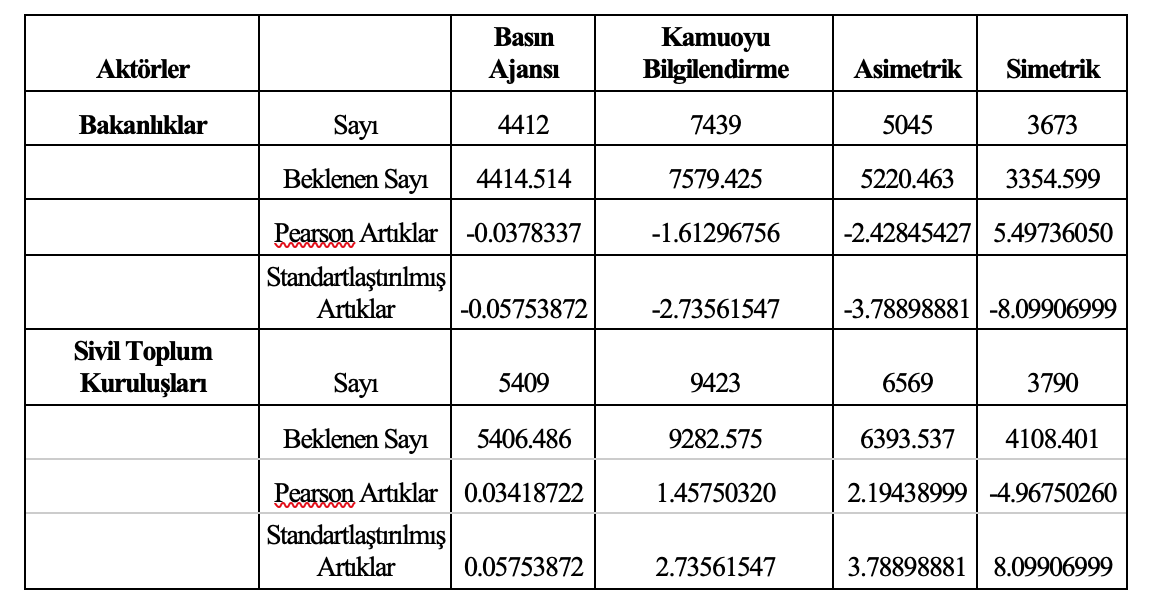
\includegraphics[width=0.95\linewidth,height=0.95\textheight]{tablolar-sekiller/tablo-4-7} \caption{Kaynak: (Mavimbela ve diğerleri, 2018: 42)}\label{fig:unnamed-chunk-11}
\end{figure}

\hypertarget{uxe7evre-ve-iklim-konu-modellemesi-1}{%
\subsection{Çevre ve İklim Konu Modellemesi}\label{uxe7evre-ve-iklim-konu-modellemesi-1}}

\textbf{AS6:} Çevre ve iklim değişikliği hakkında Türkiye'de Twitter ortamında gerçekleştirilen tartışmalarda sorun olarak görülen konular nelerdir? Bu konuların dağılımları nasıldır?

Aşağıdaki tablo 4.8'de, Türkiye'de 2020 -- 2021 yılları arasında, Twitter'da yer alan çevre ve iklim içeriklerinin konusal dağılımı yüzdelik değerler olarak gösterilmiştir. Tweetlerin konu dağılımına bakıldığında, \%19.5 ile biyoçeşitlilik konularının ilk sırada yer aldığı görülmektedir. Sırasıyla, \%13.3 iklim, \%11.7 sürdürülebilirlik, \%10.2 çevre, \%10.1 aktivizm, \%9.8 diğer, \%9.0 bilgilendirme, \%8.4 sosyal sorumluluk, \%8.0 madencilik temalarının tartışıldığı tespit edilmiştir.

\textbf{Tablo 4.8:} Konu Başlıkları ve İlgili Örnek 6 Terim.

\begin{figure}
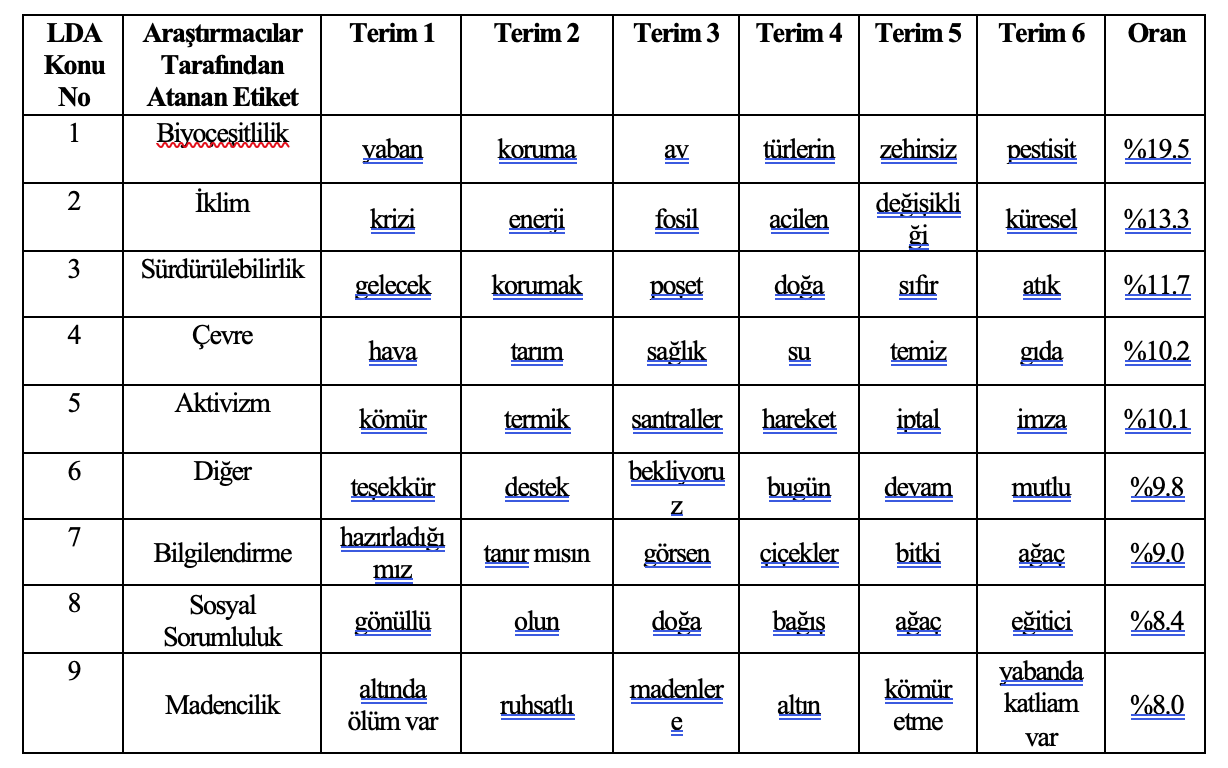
\includegraphics[width=0.95\linewidth,height=0.95\textheight]{tablolar-sekiller/tablo-4-8} \caption{Kaynak: (Mavimbela ve diğerleri, 2018: 42)}\label{fig:unnamed-chunk-12}
\end{figure}

\begin{enumerate}
\def\labelenumi{\arabic{enumi})}
\item
  Biyoçeşitlilik
  Yaşayan doğa anlamına gelen biyolojik çeşitlilik; kara, deniz ve diğer su ekosistemleri ve ekolojik yapılar da dahil olmak üzere tüm canlı organizmalar arasındaki çeşitliliği ifade etmektedir. Ekosistemlerdeki, canlı ve cansız varlıklar arasındaki yere ve zamana göre değişen genler, türler, ekosistemler ve işlevlerin tümünü kapsamaktadır (Atik, Erkoç ve Öztekin, 2010: 4). Bu tema içerisinde yaban yaşamı koruma, avcılığı yasaklanması, zehirsiz bir yaşam alanı oluşturma konuları yer almaktadır. Örnek tweetlerde (Tablo: 4.9); hayvanlar ve bitkilerle alakalı bilgilendirmeler yapılmış, doğal yaşamı koruma ve onu iyileştirme konularına değinilmiş, dünyanın insan dışında diğer türlere de ait olduğu vurgulanmış, insanların ben merkezli etnosentrik bakış açısının değiştirmesi gerektiği uyarıların da bulunulmuştur.
\item
  İklim
  İklim kategorisinde; iklim değişikliği, iklim krizi, küresel ısınma, yeşil enerji, iklim Paris Anlaşması, ikim kriziyle mücadele, adil bir değişim, fosil enerji, ekonomi, sürdürülebilir ekonomi kavramlarının yer aldığı gözlemlenmiştir. Bu terimler; iklim krizi literatürü içerisinde yer alan sorunları tanımlamakta ve iklim krizine yönelik alınacak önlemler (Ponthieu, 2020) arasında da bu terimler ön plana çıkmaktadır. Aynı zamanda; iklim eşitsizliği, enerji biçimlerinin değiştirilmesi -- yeşil enerji, iklim krizinin ekonomik etkileri vb. terimlerin her biri aynı zamanda ayrı bir çalışmanın konusu olabilecek kavramlardır.
\item
  Sürdürülebilirlik
  ``Doğa'', ``gelecek'', ``koruma'', ``sıfır atık'' ve ``poşet'' sözcüklerinin sürdürülebilirlik teması içerisinde olduğu görülmektedir. Sürdürülebilirlik fikri; doğrudan çevre ve iklim sorunlarını hafifletmek veya çözmekle ilgili olduğundan çevre ve iklim temalı birçok kelime içermektedir. Cam, kâğıt ve plastik gibi kaynakların dönüştürülmesinin önemini anlatan içerikler, sürdürülebilirliğe yönelik eylemler, geleceğin yeşil şehirlerinin oluşturulması ve avcılıkla bağlantılı içerikler de örnek tweetlerde yer almaktadır (Tablo: 4.9).
\item
  Çevre
  Bu temada; ``hava kirliliği'', ``tarım'', ``gıda'', ``sağlık'','' sıcak'', ``temiz'', ``harekete geç'' terimleri bulunmaktadır. Örnek tweetlerde (Tablo 4.9), lüzumsuz su kullanımının sonuçlarını; hava kirliliği nedeniyle sağlığı zarar görenler ya da hayatını kaybedenleri; zehirleme yapmanın verimliliği arttırmadığını aksine soluduğumuz havayı, suyu, toprağı, yediğimiz gıdaları zehirlediğini; akarsuların, dağların, toprağın neden önemli olduğunu; yanlış yatırımlarla ve çarpık kentleşmeyle birlikte doğal su kaynaklarının ve doğanın kendisinin zarar gördüğünü anlatan içerikler bulunmaktadır.
\item
  Aktivizm
  Sivil toplum kuruluşlarının yapısı gereği aktivizm temasının ön planda olması beklenen bir durumdur. Bu kategoride ``kömür'', ``termik santraller'', ``imza'', ``harekete geç'', ``iptal'' gibi terimler bulunmaktadır. Aktivizm temalı içeriklerde; genel olarak termik santraller, kömür, altın madenciliği gibi faaliyetlere son verilmesine yönelik imza kampanyaları ve etkinliklerin yapıldığı görülmektedir. İnsanların eylem yapmasını ve kamunun yararına yönelik harekete geçmelerini sağlamayı hedefleyen mesaj içerikleri tespit edilmiştir.
\item
  Diğer
  Diğer temasında genel olarak sivil toplum kuruluşlarının ``teşekkür'', ``tebrik'', ``kutlama'', ``destek'' ve ``baş sağlığı'' gibi mesajlarının yer aldığı gözlemlenmiştir. Örnek tweetlerde (Tablo 4.9), bayram ve özel gün kutlamalarını, programlara ya da katılımcılara teşekkürler mesajlarını, doğadaki canlılar ve kişiler için iyi dilek temennilerini içeren mesajlar yer almaktadır. Bu kategoride doğrudan çevre ve iklim konularına dahil olmayan mesajların kümelendiği görülmektedir.
\item
  Bilgilendirme
  Bu kategoride; genel olarak toplumun bilgilendirilmesine, toplumda farkındalık yaratılmasına yönelik mesajlarının yer aldığı gözlemlenmiştir. STK'ların takipçilerle ve diğer kişilerle etkileşeme geçmek amacıyla genelde soru cümleleriyle onları cevap yazmaya teşvik eden ya da doğrudan bir doğa olayı veya başka canlılar hakkında doğrudan bilgi veren tweetler attıkları görülmüştür. Bilgilendirme tweetlerinde; ``Bilir misin'', ``Görsen tanır mısın'', ``kuş'', ``bitki'', ``çiçek'', ``diğer hayvan ve bitkilerle'' gibi genel olarak doğa ve çevreyi ilgilendiren söz ve söz öbekleri yer almaktadır. Çevre ve iklim konularıyla ilgili bilgilendirme mesajları, halkı eğitme ve kişilerde farkındalık oluşturma amacı gütmektedir.
\item
  Sosyal Sorumluluk
  Bu kategoride daha çok, sivil toplum kuruluşlarının yapmış olduğu farkındalık çalışmaları, bağış kampanyaları, gönüllülük, sosyal sorumluluk projeleri ön plana çıkmaktadır. Bu sınıflandırmada ``gönüllü olmak'', ``bağış yapmak'', ``doğa'', ``ağaç'', ``proje'', ``çocuk'', ``eğitim'' gibi terimler yer almaktadır. Örnek tweetlerde (Tablo 4.9) doğanın korunmasına, sürdürülebilirlik etkinliklerine, proje geliştirmeye, fidan bağışlarına, su ve elektrik kullanımına yönelik eğitici tavsiyeler, sosyal sorumluluk çalışmalarına katılımı arttırmayı hedefleyen mesajlar yer almaktadır.
\item
  Madencilik
  Bu kategoride doğrudan madencilikle ilgili ``maden'', ``ölüm var'', ``kömür etme'', ``altın'', ``yabanda katliam var'' vb. terimler ön plana çıkmaktadır. Madencilik faaliyetlerine yönelik eylemler, raporlar, madencilik sektörünün zararları, madencilik iş sahasında gerçekleşen iş cinayetleri ve güvencesizlik, bu sektörün çevreye ve doğaya bıraktığı tahribat ve zararlarla ilgili içerikler yer almaktadır.
\end{enumerate}

\textbf{Tablo 4.9:} Tema Bazlı Tweet Örnekleri.

\begin{enumerate}
\def\labelenumi{\arabic{enumi})}
\tightlist
\item
  Biyoçeşitlilik\\
\end{enumerate}

\begin{itemize}
\item
  Bugün Dünya Çevre Günü🌍 Bu sene çevre gününün teması: Biyoçeşitlilik Bahçemizdeki böcekten, yol kenarındaki çimene kadar her türlü canlının birbiriyle bağlantısı vardır. Bu çeşitlilik ve bağlantı yaşamın ta kendisidir. \url{https://t.co/bCAOqquAsr}
\item
  Biyolojik çeşitliliğin anahtarı olan ormanları iyileştirmek ve halihazırda devam eden iklim krizinden etkilenen savunmasız topluluklar adına iklim adaleti aramak için dünyanın dört bir yanında çalışmaya devam ediyor. ✊
\item
  Yerkürede sadece biz yaşamıyoruz. Biyolojik ceşitliliği \#yeteryoketme \url{https://t.co/nxVqospYhF}
\end{itemize}

\begin{enumerate}
\def\labelenumi{\arabic{enumi})}
\setcounter{enumi}{1}
\tightlist
\item
  İklim * İklim değişikliği sonucu meydana gelen toprak bozulumunun milyonlarca insanı göç etmeye zorlayacağı öngörülüyor. \#ErozyonlaMücadeleHaftası Toprak hakkında merak ettiğiniz her şey için:
\end{enumerate}

\begin{itemize}
\item
  İklim değişikliği, Türkiye'de kuraklık ve çölleşme riskini her geçen gün daha da artırıyor. Türkiye'de ise ortalama sıcaklık artışı 1,5 dereceyi şimdiden geçti. Azalan yağışlar, artan sıcaklıklar ve aşırı hava olayları ile kentlerimizin direnci düşüyor.
\item
  İklim Krizinin cephe hattında, Hindistan'ın Sundarbans bölgesinde yükselen deniz adaları yutup, toprakları tuzlandırırken insanların yaşamı zorlaşıyor. Alanları daralan kaplanların da saldırıları artıyor. \#iklimkrizi \#yukselendeniz
\end{itemize}

\begin{enumerate}
\def\labelenumi{\arabic{enumi})}
\setcounter{enumi}{2}
\tightlist
\item
  Sürdürülebilirlik * 📌Karton, cam, metal ve plastiğin nasıl geri dönüştüğünü görmek için içeriklerimize göz atabilirsiniz👇 - \citet{tetrapak_tr} \citet{tcmeb} \#sıfıratık \#5D
\end{enumerate}

\begin{itemize}
\item
  ✂️ Sürdürülebilir enerji kaynakları enerjide bağımlılığı nasıl kırıyor? 📣cevap \citet{GEF_Europe} `un yayınladığı, derneğimizin çevirdiği `Yurttaş Enerjisi: Enerji Demokrasisini Gerçekleştirmek' kitabında. link: \url{https://t.co/2dUhY1bR40} \#enerji \#demokrasi \#yeşildüşünce \#gogreen \url{https://t.co/1iMAP9Bq56}
\item
  \#GreenCities, \#sürdürülebilir bir geleceği şekillendirmede çok önemli bir role sahip. Her ne kadar önümüzdeki yıl daha fazla içerikle geri dönecek olsak da Umudun Yeri Şehirler projemizin 2021 yılı faaliyetlerini özetleyerek bu yılı özetleme vakti geldi. \url{https://t.co/x4xryTMCrC} \url{https://t.co/ZTlnWZg3gl}
\end{itemize}

\begin{enumerate}
\def\labelenumi{\arabic{enumi})}
\setcounter{enumi}{3}
\tightlist
\item
  Çevre * Pestisitler iddia edilen verimliliği sağlamadığı gibi havamızı, suyumuzu, toprağımızı, yediğimiz besinleri zehirliyor. Zehirsiz hava, zehirsiz su, zehirsiz toprak, zehirsiz sofralar istiyoruz! Siz de imza verip sesimizi duyurmamıza yardımcı olabilirsiniz!
\end{enumerate}

\begin{itemize}
\item
  Dağlar neden önemli? Bitki örtüsü ve topraklar yağmur suyunu depolar, akarsuları düzenler. Dağlar insanlar için de önemlidir. Tarım, ormancılık hayvancılık, madencilik, turizm gibi ekonomik faaliyete ev sahipliği yaparken toprak kayması, erozyon ve sel gibi felaketleri önler.
\item
  Barajlarımız kuruyor. Yanlış yatırımlar, durdurulmayan kentleşme üstüne temiz su kaynaklarından geçirilmek istenen \#kanalİstanbul Suyu umarsızca üretiminde kullanan işletmeler, Yapılmayan yağmur tarımı \#ArtıkYeter \citet{karagozilker} \citet{temavakfi}
\end{itemize}

\begin{enumerate}
\def\labelenumi{\arabic{enumi})}
\setcounter{enumi}{4}
\tightlist
\item
  Aktivizm * Kirazlı Ruhsatı Durdurulsun! Çanakkale Kirazlı Siyanürlü Altın Madeni Projesi'nin ruhsatı 13 Ekim'de doluyor. Sen de ruhsatın yenilenmesine dur demek için imzala: \#KazDağlarıHepimizin \#KazDaglarınaDokunm
\end{enumerate}

\begin{itemize}
\item
  Çanakkale Yenice Çırpılar'da yapılması planlanan termik santral projesinin davası sürüyor. Santralin olası etkilerinin araştırılması ve raporlanması için yeniden oluşturulan bilirkişi heyeti ile ikinci keşif 19 Ekim Cumartesi günü Yenice'de yapılacak. \#kömüretme \#kazdağıhepimizin
\item
  Toprağımızı, gıdamızı ve geleceğimizi madenciliğe feda etmeyelim. Tarım topraklarını koruyalım. \#gıdanıkoru \#madendeğiltarım \#buyukovadamadenolmaz
\end{itemize}

\begin{enumerate}
\def\labelenumi{\arabic{enumi})}
\setcounter{enumi}{5}
\tightlist
\item
  Diğer * Doğadaki tüm dostlarımızın güvenli ve sevgi dolu bir yaşam alanına sahip olması umudu ile\ldots{} \#4EkimHayvanlarıKorumaGünü
\end{enumerate}

\begin{itemize}
\item
  \begin{itemize}
  \tightlist
  \item
    \citet{mcantonbil} Yine bir gün sabah \citet{acikradyo} da sesini duymak ümidiyle. Yol arkadaşlığın için çok teşekkür ederiz. ❤❤❤
  \end{itemize}
\item
  29 Ekim Cumhuriyet Bayramımız Kutlu Olsun🇹🇷 \#29EkimCumhuriyetBayramı \#MustafaKemalAtatürk
\end{itemize}

\begin{enumerate}
\def\labelenumi{\arabic{enumi})}
\setcounter{enumi}{6}
\tightlist
\item
  Bilgilendirme * Ülkemizdeki ilk bulgularına Oligosen Jeolojik Döneminde (34-23 milyon yıl öncesi) rastlanan kızılçam milyonlarca yıldır ülkemizde doğal olarak bulunmaktadır.
\end{enumerate}

\begin{itemize}
\item
  Bir kızılçam ağacı 20 yaşına kadar atmosferden 80 kg karbondioksit alır, 58 kg oksijen üretir. Ürettiği oksijen 142 kişinin 1 günlük tükettiği oksijen kadardır🌳\#yeşilbilgi
\item
  Bal arıları, kovanın enerji kaynağı gereksinimi için çiçeklerden veya bazı bitkilerin salgılarından nektar ve polen toplarlar. Bir işçi arının günde yaklaşık 10-24 kez nektar seferi yaptığını biliyor musunuz? Arılar hakkında daha fazla bilgi için:
\end{itemize}

\begin{enumerate}
\def\labelenumi{\arabic{enumi})}
\setcounter{enumi}{7}
\tightlist
\item
  Sosyal Sorumluluk * ``Türkiye'nin Bozkır Ekosistemlerinin Korunması ve Sürdürülebilir Yönetimi Projesi'' kapsamında Şanlıurfa'da bir dizi etkinlik gerçekleştirildi🌾 \citet{faoturkiye} \citet{FAO} \citet{theGEF} \#DKM \#natureconservationcentre \#dogakoruma \#conservationinturkey \#conservationturkey \#bozkırkoruma
\end{enumerate}

\begin{itemize}
\item
  Fidan Bağışlarınızla 2020'de 4 Mevsim Rengarenk🌳🐝 🐠🌷🦋 Yeni yılda fidan bağışında bulunun, hayatı renklerine kavuşturun🌈 Fidan bağışı için:
\item
  💧\% 4'e kadar daha az su kullanabilen su tasarruflu duş başlıkları takın. 💧Sızdıran duşları düzeltin. - \#EvdeKal \#suyukoru
\end{itemize}

\begin{enumerate}
\def\labelenumi{\arabic{enumi})}
\setcounter{enumi}{8}
\tightlist
\item
  Madencilik * Tema Vakfı, Kaz Dağları Yöresinde Madencilik adlı bir rapor yayınladı. Resmi verilere dayanan rapora göre, Kaz Dağları Yöresi'nin yüzde 79'u maden ruhsatlı.'' \url{https://t.co/NpfJPqxqSB}
\end{enumerate}

\begin{itemize}
\item
  Kaz Dağları Yöresi'nde Madencilik Raporumuz yayında. Resmi verilere dayanan rapora göre, Kaz Dağları Yöresi'nin \%79'u maden ruhsatlı! Raporun detayları için link: \url{https://t.co/xBUxNrfjRR} \#KazDağlarıRaporu \#KazDağlarıHepimizin \url{https://t.co/6esAoDfrpO}
\item
  Kömür hem madencilik sürecindeki iş cinayetleri ve güvencesizlik açısından hem de enerji üretim sürecinde sebep olduğu hava kirliliği açısından önemli bir problem. Peki gerçekten ekonomik bağımsızlık için kömüre bağımlı olmak zorunda mıyız? \#yeşildüşün \#gogreen \#greenwave
\end{itemize}

Türkiye'de, 2020-2021 yılları içerisindeki çevre ve iklim konularının tematik dağılımı yüzdelik değerler olarak belirtilmiştir. STK'ların konularının dağılımını (Şekil 4.5); sırasıyla \%19.5 ile biyoçeşitlilik, \%13.3 iklim, \%11.7 sürdürülebilirlik, \%10.2 çevre, \%10.1 aktivizm, \%9.8 diğer, \%9 bilgilendirme, \%8.4 sosyal sorumluluk, \%8 madencilik olarak tespit edilmiştir.

\textbf{Şekil 4.5:} 2020-2021 Çevre ve İklim Tweetlerin Tematik Oransal Dağılımı.

\begin{figure}
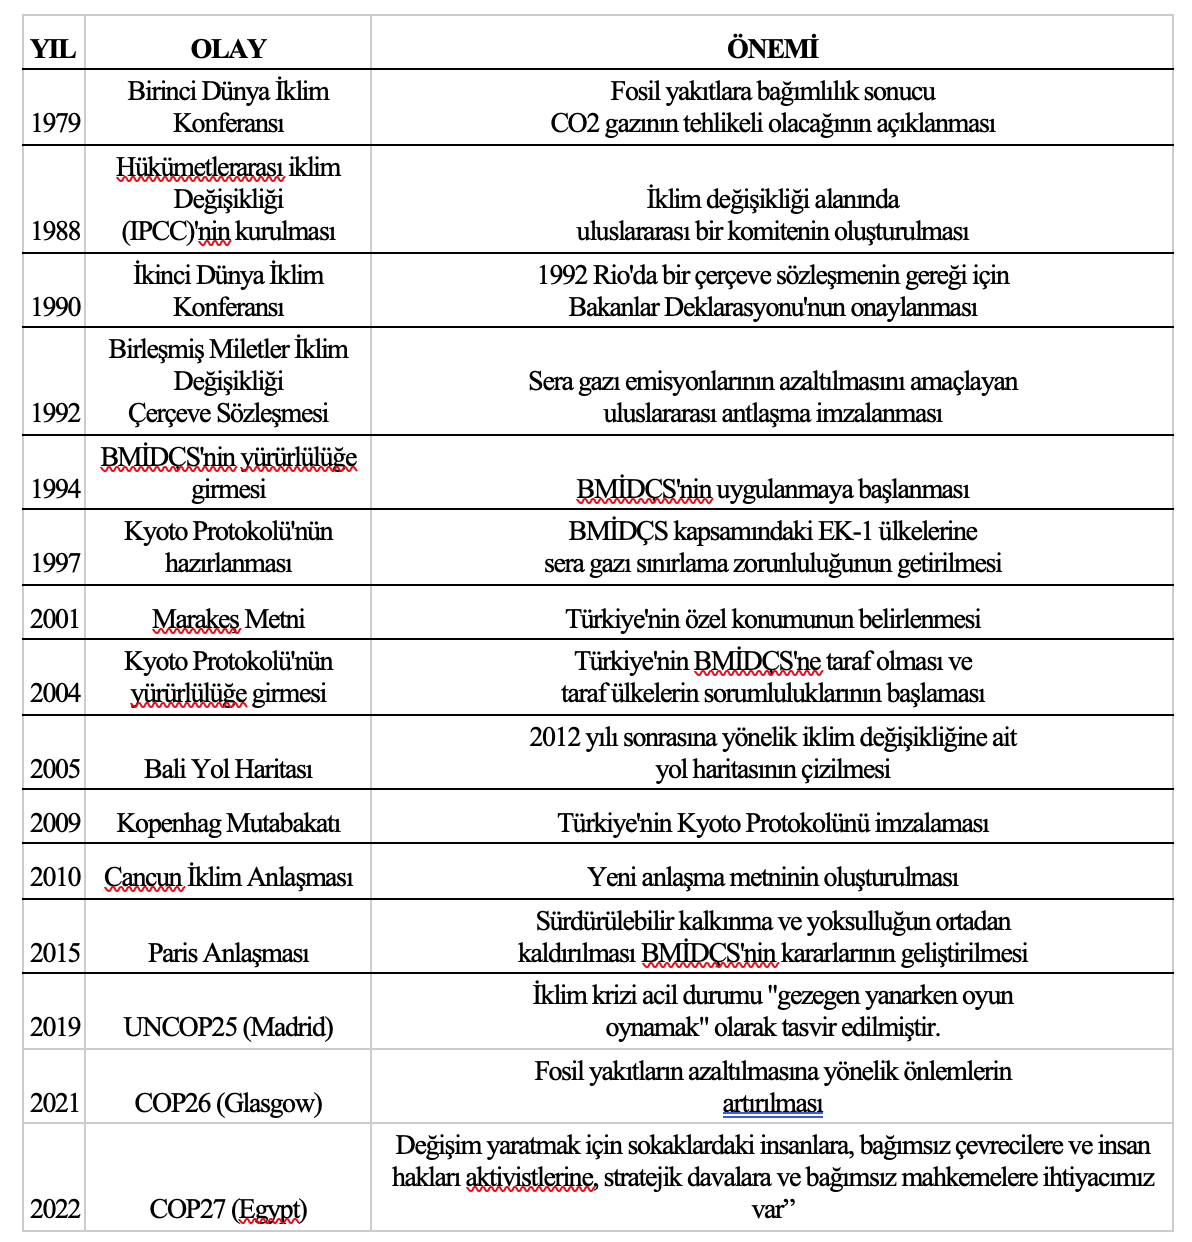
\includegraphics[width=0.95\linewidth,height=0.95\textheight]{tablolar-sekiller/tablo-2-1} \caption{Kaynak: (Mavimbela ve diğerleri, 2018: 42)}\label{fig:unnamed-chunk-13}
\end{figure}

Şekil 4.6 incelendiğinde, öne çıkan ilk üç başlık; 1) biyoçeşitlilik, 2) iklim ve 3) sürdürülebilirliktir. Bu üç konunun kesişimleri bulunmaktadır ve ortak terimlere sahip olduğu gözlemlenmiştir. Bu temalar arasındaki belirgin çizgilerin olmaması mesajların bazı durumlarda üç sınıfa da dahil olabileceğini göstermektedir. Aynı zamanda bu ilk üç temanın; X ve Y eksenlerinin kesişim noktasına yani merkeze yakın olması, sivil toplum kuruluşlarının genel olarak bu üç konu ağırlığında iletişimlerini sürdürdüğü sonucuna varılmaktadır. Çevre (4) ve aktivizm (6) temalarının kesişim noktaları olduğu görülmektedir. Genel olarak, madencilik, ağaç kesimi, HES gibi nedenlerden, çevrenin zarar görmemesi için aktivist faaliyetlerde bulunulduğundan çevre (4) ve aktivizm (6) temalarının birbirleriyle uyumlu olduğu ifade edilebilir. Kutlama, tebrik, teşekkürler gibi mesajların yer aldığı diğer (6) temasının bağımsız bir şekilde konumlandığı gözlemlenmektedir. Benzer şekilde bilgilendirme (7), sürdürülebilirlik (8), madencilik (9) temalarının da bağımsız bir şekilde konumlandığı görülse de bu temaların diğer temalara yakın oldukları da söylenebilir.

\textbf{Şekil 4.6:} Çok Boyutlu Ölçekleme Yoluyla Konular Arası Mesafe Haritası.

\begin{figure}
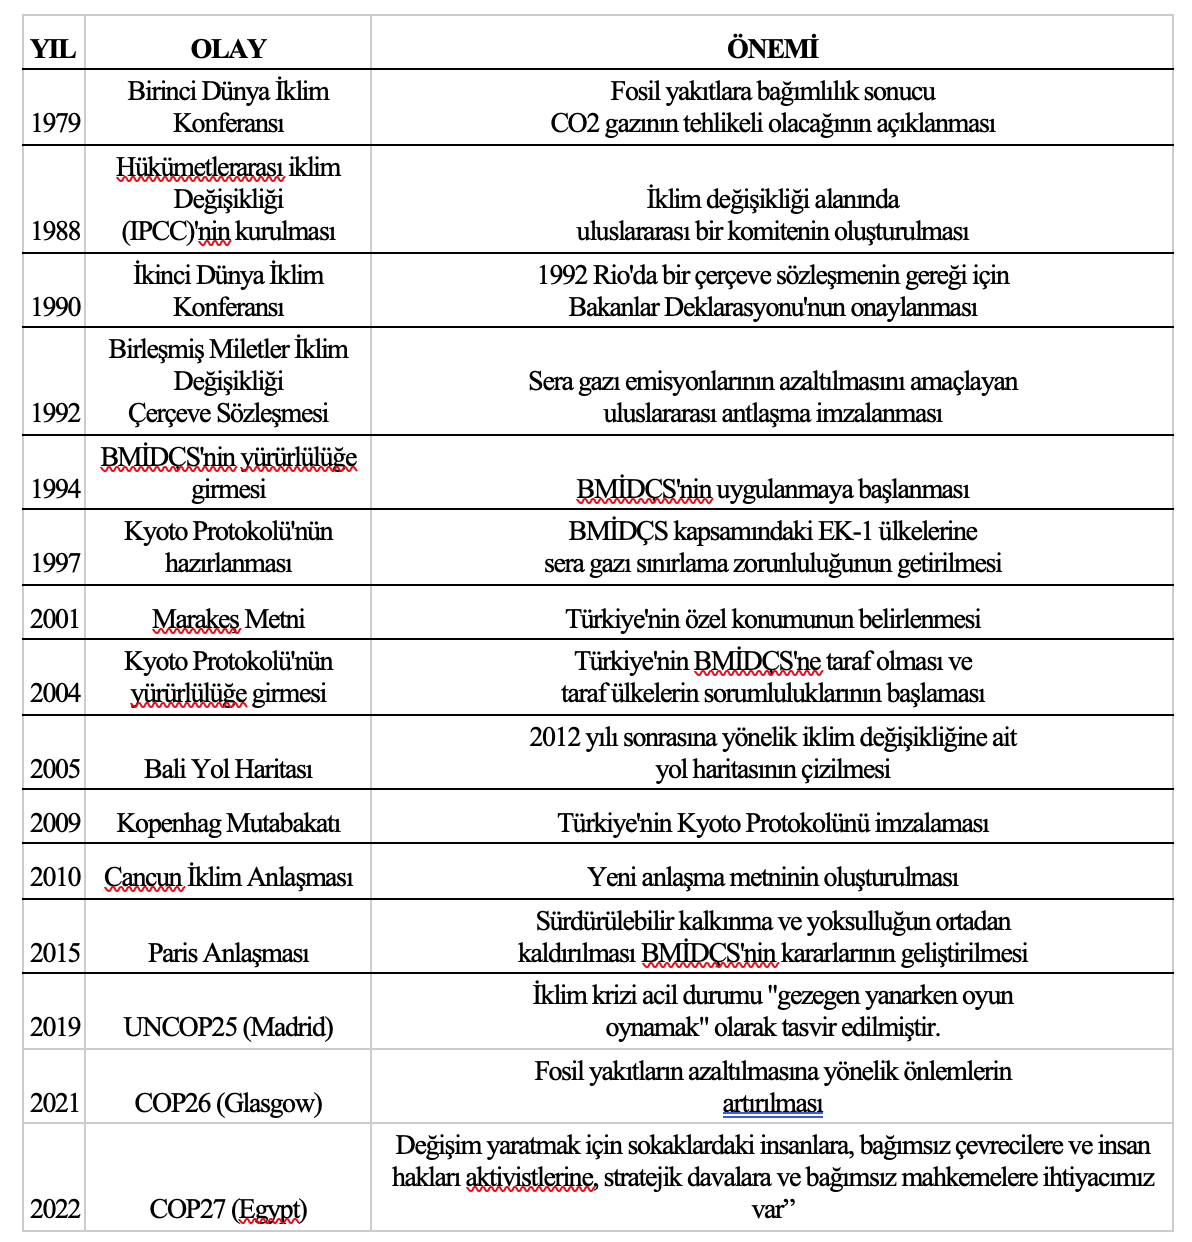
\includegraphics[width=0.95\linewidth,height=0.95\textheight]{tablolar-sekiller/tablo-2-1} \caption{Kaynak: (Mavimbela ve diğerleri, 2018: 42)}\label{fig:unnamed-chunk-14}
\end{figure}

Yukarıdaki çıktılar doğrultusunda; araştırmanın ana teması olan çevre ve iklim konuları, denetimsiz öğrenme yöntemiyle kümelendirilmiştir. Bu doğrultuda, 9 ana tema belirgin olarak öne çıkmaktadır. Tespit edilen bu konular, araştırma kapsamında belirlenen sivil toplum kuruluşlarının 2020-2021 yılları içinde; çevre ve iklim konularında attıkları tweetlerinin konu dağılımını ortaya çıkarmıştır.

\hypertarget{araux15ftux131rma-bulgularux131nux131n-deux11ferlendirilmesi}{%
\section{Araştırma Bulgularının Değerlendirilmesi}\label{araux15ftux131rma-bulgularux131nux131n-deux11ferlendirilmesi}}

Bu başlıkta, araştırma bulguları yorumlanmakta ve araştırma sorularına cevaplar aranmaktadır. Çalışma kapsamında, sivil toplum kuruluşlarının ve bakanlıkların Twitter verileri toplanmış ve incelenmiştir. Bu veriler, literatürde bahsedilen diyalojik iletişim ilkeleri ve dört halkla ilişkiler modelleri bağlamında değerlendirilmiştir. Son olarak; iklim değişikliği iletişimi bağlamında çevre ve iletişim tartışmalarının neler olduğu ortaya koyulmuştur.

Son yıllarda, iklim değişikliği üzerine sosyal medya çalışmaları artmaktadır. Özellikle Twitter, araştırmacılara; iklim değişikliğiyle ilgili etkin hesapların tespiti, temalar, söylemler, hashtagler, aktivizim ve kampanyalar gibi birçok farklı konuda çalışma imkânı sunmaktadır (Hansen ve Depoe, 2020: 171).

Araştırmanın birinci ve ikinci sorularının amacı, iklim aktörlerinin Twitter sayfalarında diyalojik ilkeleri nasıl kullandıklarını anlamak ve bu ilkeleri uygulama yöntemlerinin farklılık gösterip göstermediğini ortaya çıkarmaktır. Bu bağlamda hem sivil toplum kuruluşları hem de bakanlıklar için anahtar diyalojik ilkenin ``yeniden ziyaretçi sağlama'' olduğu tespit edilmiştir. Kuruluşların ziyaretçilerinin tekrar sayfalarına gelmelerini sağlamak için farklı sitelerden bilgi paylaşımlarına önem verdiği görülmüştür. Yeniden ziyaretçi sağlama ilkesinde, STK'ların ``ek bilgi veren sitelere'' daha çok bağlantı verdiği görülmüştür. Bakanlıklar ve STK'ların ziyaretçi geri dönüşümü ilkesi kullanımında istatiksel olarak anlamlı bir farklılık olduğu saptanmıştır.

Yeniden ziyaretçi sağlama ilkesinden sonra, aktörlerin bilginin kullanımlığı ilkesine ağırlık verdiği ortaya çıkmıştır. Bu noktada, ``fotoğraf'' paylaşımlarının ön planda olduğu görülmektedir. Fotoğrafların sosyal medya kullanıcılarının dikkatini etkili bir şekilde çekebilmesinden (Summer Harlow, Salaverría, Kilgo ve García-Perdomo, 2017) ve sosyal medya algoritmalarının görselleri ön plana çıkartma eğiliminde olmasından dolayı (Mathieu ve PavlíCková, 2017), aktörlerin bilginin kullanımlığı ilkesi doğrultusunda ``fotoğrafları'' daha çok tercih ettiği görülmektedir. Sadece ``metin'' kullanımının bilginin kullanımlığı ilkesinde ikincil olarak kullanıldığı; ``video'' kullanımının ise son sırada tercih edildiği gözlemlenmiştir. STK'ların ve bakanlıkların ``metin'', ``fotoğraf'' ve ``video'' kullanımlarında anlamlı bir farklılık bulunmuştur.

Fotoğraf \textgreater{} Metin \textgreater{} Video

Ziyaretçilerin elde tutulması kriterinde ise; STK ve bakanlıkların ``kendi websitesi paylaşımlarında'' anlamlı bir farklılık olduğu ortaya çıkarılmıştır. Bakanlıklar, kendi web sitelerini STK'lara oranla daha çok paylaşmıştır. Facebook, Youtube, Instagram gibi ``sosyal ağ sitelerinin paylaşımında'' ise STK'ların daha çok paylaşım yaptığı ortaya çıkmıştır.

Diyalojik döngü ilkesinde, ``hashtag kullanımı'' ön plana çıkmaktadır. STK'lar ve bakanlıkların ``kullanıcı etiketleme'', ``kullanıcıların cevaplanması'', ``hashtag'' kullanımlarında anlamlı bir farklılık bulunmaktadır. Bakanlıkların ``kullanıcı etiketleme'' kriterini daha çok kullandığı gözlemlenmiştir. ``Kullanıcıların cevaplanması'' ve ``hashtag kullanımı''nın sivil toplum kuruluşları tarafından daha çok tercih edildiği tespit edilmiştir.

STK ve bakanlıkların bu kapsamlı karşılaştırılması sonucunda, diyalojik ilkeleri kullanımlarının farklı olduğunu ortaya çıkmıştır. Daha spesifik olarak, bakanlıklarda için ``video'', ``kendi web sitesi paylaşımı'', ``bir tweette kullanıcı etiketleme'' ilkeleri ön plana çıkarken; STK'ların ``metin'', ``fotoğraf'', ``sosyal ağ paylaşımı'', ``ek bilgilerin alınabileceği web sitelerine bağlantılar'', ``kullanıcı tweetinin cevaplanması'', ``hashtag kullanımı'' diyalojik ilkelerine daha fazla önem verdiği görülmektedir.

Araştırmanın üçüncü ve dördüncü soruları; hedef kitlelerin beğeniler, retweetler ve yorumlar aracılığıyla Twitter'daki aktörlerle nasıl etkileşime geçtiğine; kamu katılımında beğeniler, retweetler ve yorumlar bakımından bir farklılık olup olmadığına cevap aranmaktadır. Beğeniler, retweetler ve yorumlar tweetlerin etkililiğinin önemli göstergeleridir (Wang ve Zhou, 2015). Kuruluşlar için temel diyalojik ilke olarak bilginin kullanımlığının ön plana çıktığı görülmüştür. Bilginin kullanımlığı ilkesi bakımından beğeniler, retweetler ve yorumlardan hareketle ön plana çıkan içerik türünün ``video'' olduğu tespit edilmiştir. ``Videolar''ın diğer içerik türlerine göre daha fazla kullanıcı etkileşimi aldığı ortaya çıkmıştır. Benzer şekilde, ``fotoğraf'' paylaşımlarının ``metin'' mesajlarına göre çok daha fazla etkileşim aldığı tespit edilmiştir. Ziyaretçilerin elde tutulması ilkesinde, kuruluşların ``sosyal ağ paylaşımlarının'', ``kendi web sitesi paylaşımlarına'' göre daha fazla etkileşim aldığı gözlemlenmiştir. Yeniden ziyaretçi sağlama ilkesi içinde yer alan ``ek bilgilerin alınabileceği web sitelerine bağlantıların'' beğeniler, retweetler ve yorumlarla ilişkili olduğu tespit edilmiştir. Diyalojik döngü ilkesi içinde; bir tweette ``kullanıcıları etiketlemek'' ve ``hashtag kullanımı''nın kullanıcı katılımını artırdığı görülmüştür. Bu ilke içinde etkileşimi en çok ``hashtag kullanımı''nın arttırdığı görülmüştür. ``Kullanıcı tweetinin cevaplanması''nın etkileşim değerinin düşük olduğu, gözlemlenmiştir. Bu kuruluşların belirli bir kullanıcıyı hedeflemelerinden dolayı daha az beğeni ve retweet alındığı gözlemlenmiştir. Bu gözlemin, Wang ve Yang'ın (2020) yaptığı çalışmayla uyumlu bir sonuç verdiği ifade edilebilir. Kuruluşlar, Twitter takipçilerinin dikkatini çekmeyi planlıyorsa düzenli olarak tweet yayımlayarak daha fazla beğeni, retweet ve yorum alabilirler. Böylece, kuruluşların sosyal medyadaki diyalojik iletişiminin hedef grupların katılımını artırma (Men ve diğerleri, 2018) ve onlarla ilişkilerini geliştirme potansiyeline sahip olduğu sonucuna varılabilir. Böylelikle bir ilişki geliştirme durumu ortaya çıkabilir.

Grunig'in belirttiği gibi dijital medya halkla ilişkilerin stratejik yönetim paradigması içinde diyalojik, etkileşimli, ilişkisel ve küresel özellikler barındırmaktadır (James, E. Grunig, 2009: 6). Twitter üzerinden yapılan bu araştırmada, kuruluşların ve hedef gruplarının arasındaki iletişimin bu saydığımız özellikleri taşıdığı ifade edilebilir. Kuruluşların kullanıcılarla iletişime geçmek için paylaşımlarda bulunmasının, kullanıcıların da bu içeriklerle etkileşime girmesinin, karşılıklı ilişki geliştirilmesinin ve bu mesajlara dünyanın her yerinden ulaşılabilir olmasının bu açıklamayı doğruladığı ifade edilebilir.
Araştırmanın beşinci sorusunun amacı; iklim aktörlerinin Twitter'ı, Grunig ve Hunt'un dört modeline göre iletişimlerini nasıl konumlandırdıklarını ortaya çıkarmaktır. Yapılan içerik analizi bulguları, Grunig ve Hunt'un dört halkla ilişkiler modeli bağlamında yorumlandı. Bu bağlamda, STK ve bakanlıkların Twitter kullanımları, dört model kapsamında farklılık göstermektedir. Hem STK'ların hem de bakanlıkların ``kamuoyu bilgilendirme'' modeline ağırlık verdiği gözlemlenmiştir. STK'ların ``asimetrik'', ``simetrik'' modelleri ve ``basın ajansı'' modellerini kullanımlarının bakanlıkların kullanımına oranla daha fazla olduğu saptanmıştır.

Anlaşma oryantasyonlu halkla ilişkiler; bir anlaşmazlık, problem veya kriz durumunda organizasyon ve kitle arasında uzlaşı sağlayarak bu sorunları çözmeyi amaçlar. Literatürde değinildiği gibi, iklim problemi de artık bir kriz durumu yaratmaktadır. Çevre ve iklim krizi kendini, dünyanın birçok yerinde, sayısız farklı anlaşmazlıklar, çıkar çatışmaları ile çevre ve iklim aleyhinde ortaya çıkan problemlerolarak hissettirmektedir. Bu nedenle anlaşma oryantasyonlu yaklaşım; çevre ve iklim krizinin halkla ilişkiler yönetimi sürecinde önemli bir rol oynamaktadır.

Türkiye ve Sloven Sağlık Bakanlıklarının karşılaştırmalı Twitter kullanımlarının incelendiği araştırmada, bakanlıkların \%57,5'inin basın ajansı modelini, \%35,7'sinin ise kamuoyunu bilgilendirme modellerini kullandığı tespit edilmiştir. İki ülkenin sağlık bakanlıklarının Twitter hesaplarının genel olarak tek yönlü mesajlar verdiği tespit edilmiştir (Okay, Ašanin Gole ve Okay, 2021). Bakanlıkların `'kamuoyu bilgilendirme'' modelini ağırlıklı olarak kullandığı bulgusu, Okay ve arkadaşlarının yapmış olduğu çalışmada ve bu araştırmada ortak bir sonuç olarak karşımıza çıkmaktadır.

Modellerden ilki olan basın ajansı/tanıtım modeli, halkla ilişkileri; mesajlaşma, tanıtım, bilgilendirme ve medya-ilişkileri işlevi olarak görmektedir. Bu yaklaşımı kullanarak halkla ilişkiler uygulayıcıları paydaşların davranışlarını etkilemek için ikna ve manipülasyon kullanabilirler (Mavimbela ve diğerleri, 2018: 40). Bu modelin kullanımı sonucu uygulayıcılar; genellikle eksik, çarpık veya yarı doğru bilgilerle ilgili kuruluşun yanlış inançlarını yayabilir (James E Grunig ve Hunt, 1984: 21). Basın ajansı modelinin, bahsedilen kötü yönü dışında, ikna düzeyi yüksek propaganda teknikleriyle, eğitim düzeyi düşük kitlelerde hızlı bir şekilde iklim ve çevre konularında duyarlılık oluşturabilmek mümkündür.

Grunig ve arkadaşlarının, (James E Grunig ve Grunig, 2008: 338) etnosentrik bir bakış açısıyla bir kuruluşun halkla ilişkiler stratejilerinin her ülkede aynı şekilde uygulanmasına karşı önerdikleri çok merkezli teori, çevre ve iklim konusunda da dikkate alınmalıdır. Mükemmellik teorisi; etnosentrik halkla ilişkiler ile çok merkezli teori arasında bir yerde konumlandırılmaktadır. Tüm dünyayı ilgilendiren küresel kararlarda, problemlerin çözümüne yönelik aynı kararlar dünyanın her yerinde aynı şekilde uygulanmalı, kültürel ve diğer bağlamsal koşullar göz önünde bulundurularak her ülkede ya da bölgede farklı iletişim uygulamaları göz önünde bulundurulmalıdır. Örnek olarak, WWF ve Greenpeace gibi uluslararası sivil toplum kuruluşlarının bu yaklaşımları göz önünde bulundurması yararlı olacaktır.

Mükemmellik yaklaşımı; halkla ilişkilere, kitlesel problemlerin çözümünde teorik bir yol gösterici olmakla beraber, kurumların çözüm süreçlerini hedef kitlelerle ortak anlayış içinde sürdürmelerini ve karşılıklı bilgi akışını sağlıklı yönetmelerini sağlamaktadır. Mükemmellik teorisi, her ne kadar kurumsal düzeyde ele alınmış olsa da çevre ve iklim problemlerinin ele alınmasında, hedef gruplarının bu problemlerin çözümüne dahil edilmesinde iletişim çalışmaları için yol göstericidir. İklim krizi yalnızca devletlerin, kurumların çözebileceği bir problem olmadığından toplumun da çözüm sürecine dahil edilmesi gerekmektedir. Bu noktada, literatürde değinilen iklim hedef grupları göz önünde bulundurularak bu grupların bilinçlendirilmesi, çözümün bir öznesi oldukları hissettirilmesi ve onlarla bu yollarla iletişim kurulması önemlidir.

Araştırmanın altıncı sorusunun amacı; çevre ve iklim değişikliği hakkında Türkiye'de Twitter ortamında gerçekleşen tartışmalarda sorun olarak görülen konuların neler olduğunu ve dağılımını ortaya çıkarmaktır. Yapılan konu modellemesi sonucunda, STK'ların paylaşımlarının 9 ana başlıkta kümelendiği gözlemlenmiştir. Biyoçeşitlilik, iklim ve sürdürülebilirlik temalarının diğer temalara göre merkeze daha yakın ağırlıkta olduğu tespit edilmiştir. Literatürde yer aldığı gibi STK'ların iklim krizinin ve bileşenlerinin ana konular olarak yer aldığı ortaya çıkmıştır. Literatürde değinilen iklim krizinin zorlukları (Leal Filho ve diğerleri, 2019) mesajların geniş kapsamı ve tema çeşitliliği bu analizde de görülmektedir. Birbirleriyle doğrudan ilişkili birçok tema bulunmaktadır. Sürdürülebilirlik; çevre ve iklim temalarıyla doğrudan bağlantılıdır. Aynı zamanda, madencilik faaliyetleri hem çevreye ve iklime hem de biyolojik çeşitliliğe büyük zararlar vermektedir. Bu temalar birbirinden bağımsız düşünülemez. Hedef gruplarının karmaşıklığı, ilgi odaklarının farklılığı ve iklim iletişiminde bulunan zorluklar, iklim krizine konsolide bir toplumsal destek sağlamayı zorlaştırmaktadır. Her hedef grubunun zihinsel çerçeveleri ve odak noktaları çok geniştir. Bu sebeple, iklim mesajlarının kapsamlarının ve temalarının belirlenmesi ile raporlanması sürecinde her bir hedef kitlenin zihin çerçevelerinin ve odak noktalarının dikkate alınması, başarılı bir iletişimin gerçekleştirilmesini mümkün kılacaktır. Bulgular, STK'ların çevre ve iklim konularında toplumu eğitmeye, toplumda farkındalık oluşturmaya ve diğer unsurlar üzerinde bir baskı unsuru olmaya yönelik aktivist hareketleri destekledikleri ifade edilebilir.

Filho'nun belirttiği gibi (Leal Filho, 2019: 4), iklim değişikliği iletişimi, toplumu eğitmekle ve bilgilendirmekle mükelleftir; bunu yapmak için insanların iklim krizi sonucunda kendi çevresinin hangi riskler altında olduğunu, küresel ölçekteki sorunun yereldeki etkilerini; su, enerji kullanımı, ulaşım gibi günlük rutinlerin etkili ve uygun bir şekilde kullanımını doğru ve eksiksiz öğrenebilmeleri için iyi bir iletişim stratejisi gerekmektedir. Ek olarak; iklim değişikliği bir yönetişim sorunudur ve uzun vadeli bir planlama gerektirmektedir. Dört yıllık bir seçim döngüsüne veya bakanların, üst düzey yetkililerin iki ya da üç yıllık görev sürelerine göre şekillenemez. Günlük siyasetin ritmine pek uymamaktadır.

Konu modelleme çıktılarının; çevre iletişiminin çalışma alanındaki temalarla da uyum içinde olduğu gözlemlenmektedir (Cox ve Pezzullo, 2018: 36). Kişilerin çevresel tutumlarını, tüketim alışkanlıklarını, eğitim uygulamalarını kapsayan Çevresel Kişisel Kimlik ve Kişiler Arası İlişkiler (1) alanıyla, çalışmanın kendisinin, belirli kurumların ya da ağların çevresel konuları nasıl tartıştığını ve örgütlendiğini araştıran Çevresel Organizasyonel İletişim Çalışmaları (2) alanı içinde yer aldığı ifade edilebilir. STK'ların söylemleri içerisinde, onların var olma nedenlerinden biri olan Çevresel Karar Alma Süreçlerine Toplumsal Katılımı (4) sağlama çabasında olduğu görülmektedir. Son olarak, bu araştırmanın sözlü-sözsüz etkileşimleri araştıran Çevresel Retorik ve Kültürel Çalışmalar (7) alanlarını kapsadığını da ifade etmek mümkündür.

Üçüncü bölümde değinilen ``Çevre İletişim Bilgi Modeli'' ve ``İletişim Sürecinin Ekolojik Modeli'' iletişim modelleri bağlamında daha genel kapsamda kullanılmasından dolayı, geniş kapsamlı çevre ve iklim konularında Çevre İletişim Bilgi Modeli'nin; İletişim Sürecinin Ekolojik Modeli'nin ise daha yerel konumlarda kullanılması daha uygun olacaktır (Jurin ve diğerleri, 2010: 19). İklim aktörlerinin mesajlarını oluştururken bu modelleri göz önünde bulundurmaları daha etkili bir iletişim kurmalarını sağlayabilir.

İletişim çalışmalarında ve sosyal bilimlerin diğer alanlarında, yeni dijital veri kaynaklarına dayalı araştırmaları sürdüren çeşitli disiplinler arasında diyaloga ihtiyaç duyulmaktadır (Schroeder ve Schroeder, 2016). Bu araştırmada gözlemler, veri bilimi içerisinde yer alan yöntem ve teknikler, iletişim bilimlerinin bir alanı olan halkla ilişkiler teorileri kapsamında değerlendirilip yorumlanmıştır.
LDA konu modellemesi, büyük metin verilerinde bir içgörü elde etmemizi sağlamaktadır. Bu yaklaşımın veri odaklı ve hesaplamalı doğası onu iletişim çalışmaları için önemli kılmaktadır. Çünkü, büyük miktardaki metin verilerinin tematik yapısının hızlı ve verimli bir şekilde ortaya çıkmasını sağlamaktadır. Tümevarımsal bir yaklaşımı, nicel ölçümlerle birleştirerek onu keşfedici ve tanımlayıcı analizler için uygun hale getirmektedir (Maier vd., 2018: 93). Uluslararası iletişim literatüründe, konu modellemeyle ilgili örnekler bulunmaktadır (Chae \& Park, 2018; Maier vd., 2018; Xie vd., 2022). Türkçe literatürde LDA ve benzeri yaklaşımların mühendislik, davranış bilimleri vb. alanlarında çalışıldığı gözlemlenmiştir (Ekinci \& Omurca, 2017; Onan vd., 2020; Sobaci vd., 2022). Sosyal medyadaki veri akışı, farklı türdeki veri yapıları ve dijital teknolojilerin dinamik gelişimi, araştırmacılar için geniş olanaklar sağlamaktadır. Yurt dışı üniversitelerde dijital methodlarla ilgili alanlarda çalışma grupları yer almaktadır
.\\
İklim değişikliği ile ilgili eylemlerin, tüm sektörel etkileri ve politika bileşimleri incelenmeli ve yeni çözüm yolları araştırılmalıdır. Mevcut sanayi stratejisi, ticaret politikası, rekabet politikası, yenilik politikası, işgücü politikası ve mali düzenleme ve diğer politikalar içinde iklim politikalarının uygulanmasının önünde yer alabilecek engeller incelenmeli ve gerekli değişiklikler yapılmalıdır. İklim değişikliği politikalarına uyumlu bir ekonomiye ulaşmak için tüm politika alanları koordine edilmelidir (Ponthieu, 2020: 79). İklimi iyileştirmek için etik boyutta, bundan sonraki süreçte hayvancılık adı altında yapılan ticaretin sonlandırılması, et tüketimi kültürü ve eşitsizlik üzerine kapsamlı çalışmaların yapılacak olması muhtemel görünmektedir. Sürdürülebilir bir dünya için iklimi önemseyen toplumlar inşa edilmelidir. Bu vizyon sektörel politikalardan çok daha fazla önemsenmelidir. Uzun vadeli vizyon geniş iş birlikleriyle desteklenmesini, ülkeler arasındaki gelişmişlik düzeyinin en alt seviyeye çekilmesini gerektirmektedir. Özel sektör katılımını daha fazla çekmek için döngüsel ekonomi ve paylaşım ekonomisi başta olmak üzere yeni sürdürülebilir ekonomik modellere geçiş yapılmalıdır. Ayrıca, çevre dostu teknolojilerin ve çalışma ortamlarının geliştirilmesini teşvik etmek önemlidir.\\
Huang ve Lin'in (Huang ve Lin, 2022) kurumsal sosyal sorumluluk üzerine yaptığı çalışma; iklim krizi algısının yüksek olduğu bölgelerde organizasyonların kurumsal sosyal sorumluluk uygulamalarına daha fazla önem vermesi için toplumun iklim aktörleri tarafından daha fazla bilgilendirilmesi, eğitilmesi ve onların da bu iklim eyleminin bir parçası olduğunu hissettirmek adına aktif katılıma yönelik iletişim stratejileri geliştirmenin önemini göstermektedir.

Ponthieu (Ponthieu, 2020: 95- 96) iklim krizi politikalarına yüksek düzey katılımın olması ve bu politikaların tutum haline gelmesi için kültürel hassasiyetler göz ardı edilmeden iklim politikalarının yerel ortamlara bütünleşmiş bir şekilde yürütülmesinin önemini vurgulamaktadır.

Günümüzde, temel ekonomik sistemin verimsizliği ve zayıflıklarıyla her geçen gün daha fazla yüzleşmekteyiz. Ekonomik modellerde derinlemesine bir reformun gerekliliğiyle karşı karşıyayız. Bu bağlamda, sivil toplum kuruluşları bu ekonomik modelin değişmesi gerektiğine dair temel bir baskı unsuru oluşturmaktadır. Günümüz ekonomik sisteminin işlevsizliği hakkında fikir birliği bulunmasına rağmen problemin çözülmesine yönelik bir çalışma bulunmamaktadır.

Daha önce yapılan çalışmalar göstermektedir ki, çevre ve iklim; ilk bakışta dikkat çekmeyen, kavranması ve anlaşması zor bir konudur (Mahl ve diğerleri, 2020). Üçüncü bölümde değinilen iklim değişikliği iletişimi zorlukları ve hedef grupları göz önünde bulundurularak yapılacak iletişim çalışmaları konunun özümsenmesine yardımcı olacaktır.

Bireysel yaşam tarzı düzenlemeleri; iklim değişikliğine tam bir çözüm olmasa da; bireysel davranışları, tutumları ve düşünceleri değiştirmeye odaklanan iletişim stratejilerinin kamuoyu oluşturması, ilgili aktörlerin eylemlerine baskı unsuru olması, onları denetlemesi, iklim ve çevre konularına yönelik duyarlılığın daha geniş bir sosyal alana yayılması gibi birçok faydası olacaktır (Hansen et al., 2016: 31).

\hypertarget{sonuuxe7-ve-tartiux15fma}{%
\chapter*{SONUÇ VE TARTIŞMA}\label{sonuuxe7-ve-tartiux15fma}}
\addcontentsline{toc}{chapter}{SONUÇ VE TARTIŞMA}

Dijital medya; halkla ilişkilerin stratejik yönetim paradigması için mükemmel bir şekilde uygun olan diyalojik, etkileşimli, ilişkisel ve küresel özellikleri içermektedir (James, E. Grunig, 2009: 6). Twitter gibi mecralar hem organizasyonlar hem de hedef grupları arasında Grunig'in gösterdiği bu özellikleri taşımaktadır. Sosyal ağlar üzerindeki hareketlilik, veri miktarı, farklı veri yapıları ve teknolojinin dinamik gelişimi araştırmacılar için muazzam bir çalışma alanı sunmaktadır.

Halkla ilişkiler; imaj, algılar, mesajlaşma, itibar, markalar, entegre pazarlama iletişimi, yatırım getirisi (ROI), stratejik iletişim, kurumsal sosyal sorumluluk projeleri gibi kavramlara odaklanmaktadır. Halkla ilişkiler uygulayıcıları, yeni dijital medyayı; düşünme biçimlerini değiştiren ve halkla ilişkiler uygulamalarını şekillendiren devrimci bir güç olarak görmektedir (s. 1). \citep{grunig2009paradigms} Organizasyonlar; halkla ilişkiler uygulamalarını, pazarlama faaliyetlerini ve diğer iletişimlerini sosyal ağlar üzerinden sağlamaktadır. Bu nedenle, sosyal ağ uygulamalarından Twitter, halkla ilişkiler çalışmaları için verimli bir kullanım alanı olarak karşımıza çıkmaktadır.

Sosyal medya kuruluşların hedef kitleleriyle ilişkiler kurmaları için bir platform sağlamaktadır. Araştırma kapsamında, sivil toplum kuruluşlarının ve bakanlıkların Twitter sayfalarında; diyalojik ilkeleri kullanma biçimleri incelenmiş ve kullanım kalıplarını karşılaştırılmıştır. Bu araştırma, kuruluşların diyalojik iletişimini ve hedef kitlelerinin katılımını birleştirmeye yönelik öncü çalışmalardan biridir. Aynı zamanda, elde edilen veriler; Grunig-Hunt'un dört halkla ilişkiler modeli bağlamında yorumlanmıştır. Son olarak, çevreci sivil toplum kuruluşlarının 2020 -- 2021 yılları arasındaki paylaşımlarının içerdiği temalar, LDA konu modelleme analiziyle ortaya koyulmuştur.

Twitter üç nedenden dolayı tercih edilmiştir: 1) Küresel şirketler tarafından en yaygın kullanılan sosyal medya kanalı olması. 2) Diyalojik iletişim için mention, hashtag, media, linkler gibi birçok faydalı özellik sunması. 3) Hemen hemen tüm kurumların Twitter sayfalarına herhangi bir kullanıcı tarafından erişilebilir olmasıdır.
Son dönemlerde diyalojik iletişim üzerinde yapılan çalışmaların, Twitter gibi sosyal ağ uygulamaları üzerinde yapıldığı görülmektedir. Thelen ve arkadaşları;112 halkla ilişkiler ajansının Twitter paylaşımlarını, diyalojik iletişim bağlamında ele almışlardır. \citep{thelen2021dialogic} Bir diğer araştırma ise hem kar amaçlayan hem de kar amacı olmayan kuruluşların tweetlerini, diyalojik iletişim olgusu çerçevesinde karşılaştırmıştır (Wang ve Yang, 2020). İklim aktörlerinin diyalojik unsurları ne ölçüde kullandığı araştırılmıştır. Araştırma tasarımı oluşturulurken bu iki makaleden de faydalanılmıştır. Diğer bir araştırmada ise Fortune 500 şirketlerinin Twitter profillerinin içerik analizi yapılmıştır. \citep{rybalko2010dialogic}

\citet{kent1998building} çalışmalarında, organizasyonların ve hedef gruplarıyla web üzerinden diyalojik iletişim kurmaları için bir çerçeve sunmaktadır. Diyalojik iletişim olgusu, halkla ilişkilerin simetrik modeli ile ilişkilendirilmektedir. İki yönlü halkla ilişkiler modelini uygulayan organizasyonlar; problemleri sonuçlandırmak, karşılıklı anlayışı geliştirmek ve hedef gruplarıyla bağ oluşturabilmek için diyalog kurmaktadırlar. Sosyal medyanın yorumlanması ve değerlendirilmesi bakımından diyalojik iletişim önemli bir kuramsal çerçeve sunmaktadır.

\citet{kent1998building}'un diyalojik iletişim için ortaya koyduğu beş unsur, web sitelerinin teknik ve yapısal unsurlarını ortaya koymaktadır. Kurumların, diyalojik iletişim kurmak için web sitelerinde bu unsurlara dikkat etmeleri önem arz etmektedir. Sosyal medya üzerindeki halkla ilişkiler uygulamalarında da diyalojik iletişim kullanılmaktadır. Reklam ve pazarlamaya yönelik tek yönlü iletişim faaliyetleri dışında, sosyal medya sayesinde organizasyonlar ve hedef grupları arasında karşılıklı bir diyalog ve etkileşim ortamı oluşmuştur. Literatürde değinilen süreçler, web sitelerinin kolay kullanılabilirliği, mobil uyumlu olması, hızlı çalışması, blog, sosyal ağ uygulamalarında vakit geçirilmesini sağlayabilecek içeriklerin üretilmesi gibi unsurları kapsamaktadır. Kullanıcı dostu içerikler paylaşılırken ziyaretçilerle iletişimin devam etmesi için soru, görüş ve yorumlar gibi karşı taraftan gelebilecek geri dönüşlere de açık olunması ve kullanıcıyla diyalog oluşması ve halkla ilişkiler faaliyetleri açısından da önem arz etmektedir.

Araştırmanın birinci sorusu ile hem sivil toplum kuruluşları hem de bakanlıklar için anahtar diyalojik ilkenin ``yeniden ziyaretçi sağlama'' olduğunu tespit edilmiştir. Kuruluşlar ek bilgi veren siteleri paylaşarak bunu sağlamaktadır. İkincil olarak ``bilginin kullanımlığı'' ilkesine ağırlık verildiği, bunun da ``fotoğraf'' paylaşımlarıyla yapıldığı tespit edilmiştir. ``Ziyaretçilerin elde tutulması'' kriterinde ise bakanlıkların ``kendi websiteleri paylaşımlarına'' öncelik verdiği, STK'ların ise daha çok ``sosyal ağ paylaşımları'' yaptığı ortaya çıkmıştır. Kuruluşların ``diyalojik döngü'' ilkesi kullanımlarında da belirgin farklılıklar olduğu gözlemlenmiştir. STK'lar ``kullanıcıların cevaplanması'' ve ``hashtag kullanımı'' özelliklerini daha fazla kullanırken bakanlıklar ise ``kullanıcı etiketleme'' özelliğini daha fazla kullanmıştır.
Kuruluşların diyalojik iletişiminin halkın katılımı üzerindeki etkisine odaklanan üçüncü ve dördüncü araştırma sorularından; kuruluşların diyalojik iletişim ilkelerinin kullanımlarıyla ve kamu katılımının arasında güçlü bir ilişki olduğu sonucu çıkmıştır. Beğeniler, retweetler ve yorumlar, kuruluşların tweet etkililiğinin önemli göstergelerindendir. Etkililik kapsamında ``bilginin kullanımlığı'' ilkesi ön plana çıkmıştır. Bilginin kullanımlığı kriterinde, en çok katılımın ``video'' içerik türüyle sağlandığı ortaya çıkmıştır. Aynı şekilde, ``fotoğraflar'' en çok etkileşim alan ikinci içerik türü olarak tespit edilmiştir. Aktörler tarafından en az kullanıma sahip içerik türü ``video'' olmasına rağmen en fazla etkileşim alan medya türü olarak karşımıza çıkmaktadır.

Diyalojik iletişim üzerine yapılan araştırmanın sonuçları; Phillips'in sosyal medyanın halkla ilişkiler uygulamalarına uygun diyalojik, etkileşimli ve ilişkisel özellikler barındırdığı savını doğrular niteliktedir. Araştırma çıktılarından anlaşılan; halkla ilişkiler uygulayıcılarının geleneksel olarak tek yönlü iletişim, mesaj odaklı ve asimetrik iletişim yerine, simetrik bir iletişim tercih etmelerinin daha uygun olacağıdır. Araştırma bulguları, diyalojik iletişimle ilgili önceki çalışmalarla benzerlikler göstermektedir. Etkileşimle ilgili yapılan testlerde, ``yorumların cevaplanması'' kriterinin sadece tek bir kullanıcıyı hedeflemesinden dolayı, etkileşim değerinin diğer ilkelerden düşük bulunması diğer çalışma sonuçlarıyla da \citep{wang2020dialogic} paralellik göstermektedir.

\citet{mahl2020bit} ve arkadaşlarının çalışmalarında belirttikleri gibi, çevre ve iklim değişikliğine yönelik algılar, iletişim stratejileri kurumların desteğinin artmasını ve bireylerin tutum ve davranışlarının değişmesini sağlayabilir. Çevre ve iklim konularında, kamunun politikalara desteğinin artması açısından iklim aktörlerinin söylemlerini, belirli bir iletişim stratejisine uygun şekilde oluşturmaları önerilmektedir. Yapılan içerik çalışmasında, video içeriklerinin kullanıcı etkileşimini artırdığı görülmüştür. Bu doğrultuda, iklim değişikliği iletişimi kapsamında eğitici, farkındalık yaratan video içeriklerinin oluşturulması önerilebilir. İklim değişikliği iletişim süreçlerinde genelde ``bilgilendirme'' ve ``eğitim'' bileşenlerine odaklanıldığı, nadiren ``teşvik etme'' ve ``izleme'' faaliyetlerinin göz önünde bulundurulduğu belirtilmektedir (s. 5). \citep{leal2019overview} İklim değişikliği iletişim süreçlerinin başarısı için ``izleme'' bileşeninin de bu süreçlere dahil edilmesi önem arz etmektedir.

İklim aktörlerinin, Twitter'da Grunig ve Hunt modellerini nasıl konumlandırdıklarıyla ilgili yapılan araştırmanın bulguları, modellerin kullanımlarında parallelikler olduğunu göstermektedir. Her iki aktör grubunda en çok kullanılan modeller; kamuoyu bilgilendirme modeli, asimetrik model, basın ajansı, ve simetrik model olarak sıralanmaktadır. En az kullanılan modelin simetrik model olduğu görülmektedir. Her iki aktör grubunun model kullanımlarında parallelik bulunmasına rağmen, kullanım sıklıklarında farklılıklar olduğu görülmüştür. STK'ların bakanlıklara göre, asimetrik ve simetrik iki yönlü modelleri daha fazla kullanma eğiliminde olduğu ifade edilebilir.
İklim teması üzerine yapılan önceki çalışmalarda; küresel iklim krizinin toplumlar tarafından farklı algılanmaması, bu konuda bir fikir birliğine varılması ve ortak hareket edilmesi gerekliliğinden yola çıkarak 2009 ile 2018 yılları arasında oluşturulan \#climatechange (\#iklimdeğişikliği) ve \#globalwarming (\#küreselısınma) hashtaglerini içeren 6.662.478 tweete dayanarak iki söylemin (iklim değişikkliği ve küresel ısınma) anlamsal ağları ve on yıl içindeki antropolojik evrimi incelenmişlerdir. Araştırma sonucuna göre; küresel ısınma kavramının daha politize açıklamalar için kullanıldığı; iklim değişikliği kavramının ise daha çok bilimsel açıklamalar için kullanıldığı gözlemlenmiştir. , 20 \citep{shi2020climatechange}

Bir diğer araştırmada, iklim değişikliğiyle ilgili medya söylemlerini araştırmak için Litvanya'da 2017 -- 2018 yılları arasında yayımlanan 583 haber makalesi konu modelleme yaklaşımıyla incelenmiştir. Medya söyleminin ulusal ve uluslararası bağlantıları araştırılmıştır. Araştırma sonucu; Litvanya medyasının iklim krizini uluslararası ölçekte güçlü bir şekilde ele aldığını, ulusal ölçekte de bu krizin daha fazla gündemde yer almasının altı çizilmiştir (Rabitz vd., 2020). Üçüncü bölümde bahsedilen ``tema sorumluluğu'' ve ``coğrafi dağılım'' iklim iletişimi zorlukları, bahsedilen Litvanya medyası çalışmasında da görülmektedir.

İklim değişikliği iletişimi üzerine yapılan araştırma sonuçları, iklim değişikliğine ilişkin bireysel algıların; halkın, medyanın ve diğer bilgi kaynaklarının konuyu nasıl tasvir etme biçiminden güçlü bir şekilde etkilendiğini göstermektedir. Buna göre bu bilgi kaynakları; iklim değişikliğinin üretiminde, yeniden üretiminde ve anlamının dönüştürülmesinde rol oynayan önemli faktörlerdir (Mahl ve diğerleri, 2020). \citep{mahl2020bit}

Günümüzde dünya çapında, daha sık ve yoğun doğal afetler üreten aşırı hava koşulları görülmektedir. İletişim, tahmin, hazırlık, azaltma, önleme, iyileştirme, esneklik uygulamaları, her krizde ve her noktada önemli birer rol oynamaktadır. 21. yüzyıl; dünya ve sosyal bilimcilerin, bireylerin ve toplulukların doğal afetlerden hızla kurtulma kapasitelerini geliştirmeleri için birlikte çalışmalarını gerekli kılmaktadır. Dolayısıyla çok disiplinli bir bakış açısına ihtiyaç duyulmaktadır (s. 2). \citep{drake2016communicating} Bu kapsamda, çalışmanın çok disiplinli bakış açısına katkı sunması beklenmektedir. Aynı zamanda, çalışmada iklim aktörlerinin daha iyi bir iklim değişikliği iletişimi kurmasını sağlayacak yararlı bilgiler ortaya koyulmuştur.

Araştırmanın sınırlılıkları olarak; bu çalışmada Twitter verileri üzerinde bir otomatikleştirme çalışması gerçekleştirilmiştir. Bu, büyük miktardaki verilerin analizini hızlı ve etkili bir şekilde yapabilmeyi mümkün kılmaktadır. Araştırma için elde edilen veriler, Twitter üzerinde akan verilerle sınırlıdır. Twitter'ın arayüzü, kullanıcı bilgileri, sosyal ağlar ve web siteleri gibi dış bağlantı bilgilerinin kendi içerikleri analize dahil edilmemiştir. Elde edilen içerikler, araçsal olarak diyalojik ilkeler ve dört model; bu bağlamda değerlendirmelere tabi tutulmuştur. Son olarak; konu modelleme analizi için iki yıllık zaman periyodu yerine, altı aylık ya da senelik zaman aralıklarıyla çalışılarak; konuların değişim oranları üzerine daha detaylı bir sonuç almak mümkündür. Örneğin, son altı ayda sel baskınları, kamu arazilerinin yağmalanması gibi konular gündemde ise bu konuların incelenen zaman periyodu içerisinde ön plana çıkması olasıdır. Bu zaman aralığı, kapsamı, araştırmacının amacı doğrultusunda belirlenebilir. Aktör bazlı bir çalışma yapılacaksa; her bir aktörün veri miktarının birbirine yakın olması, aradaki benzerlikleri ve farklılıkları ortaya çıkarmak için daha sağlıklı bir ortam sağlayacaktır. Bir aktörün veri miktarının (örneğin: tweet sayısı) diğer aktörlerden fazla olması araştırmada yanlı bir sonuç çıkmasına sebebiyet verebilmektedir. Yapılacak araştırmaların amacına göre, bu farklı yaklaşımların göz önünde bulundurulması gerekmektedir.

Dijital çağda, trendler hızla değişmektedir ve halkla ilişkiler uygulayıcılarının yeni bir halkla ilişkiler aracı olarak gördükleri uygulamaların merkezinde sosyal medya bulunmaktadır. Uygulayıcılar; halkla ilişkiler çalışmalarında yenilikler yaratmak için sosyal medyayı nasıl kullanabileceklerini tartışan konferanslar, seminerler, çevrimiçi tartışmalar, yayınlar, kitaplar, web siteleri ve bloglar yapmaktadırlar. Grunig, sosyal medyanın tam anlamıyla kullanılması halinde halkla ilişkilerin küresel, stratejik, iki yönlü ve etkileşimli, simetrik ya da diyalojik ve sosyal olarak sorumlu hale gelebileceğini belirtmiştir. \citep{grunig2009paradigms}

Bu çalışma, diyalojik iletişim ilkelerini \citep{kent2002toward} dijital medya bağlamına uyarlayıp geliştirerek alana katkı sağlamaktadır. Çalışmada geliştirilen araştırma yaklaşımı, diğer organizasyon türlerine (örneğin: şirketler, diğer kamu kuruluşları, kanaat önderleri) ve sosyal sorumluluk, kriz iletişimi gibi diğer bağlamlara uyarlanabilir. Bu çalışmada da ele alınan yaklaşım Grunig-Hunt'un dört halkla ilişkiler modelinden uyarlanmıştır. Aynı zamanda, çalışma diyalojik iletişim ve sosyal medyada kamunun katılımının incelendiği öncü çalışmalardan bir tanesidir. Bu özelliği ile gelecekteki araştırmalar için bir yön sağlayacağı düşünülmektedir. Aynı zamanda hükümet kanadından bakanlıkların ve sivil toplum kuruluşlarının Twitter kullanımının hedef kitleleriyle ilişkiler kurarken diyalojik iletişim ilkelerini takip etme açısından nasıl farklılaştığını araştıran ilk araştırmalardan bir tanesidir.

Literatürde de değinildiği gibi çevre ve iklim konularını anlatmak ve farkındalık oluşturmak için sosyal bilim araştırmacılarına büyük görevler düşmektedir. Çevre ve iklim değişikliği iletişimi bağlamında, daha etkili iletişim stratejilerinin oluşturulması için iletişim araştırmacılarının daha fazla çalışma yapmaları gerekmektedir. Mesajların kitlesel olarak yayılabildiği sosyal medya platformlarının üzerinden çevre ve iklim değişikliği sorunlarına yönelik olarak ikna etme gücü, algı oluşturma, farkındalık yaratma, tutum ve davranış değiştirme üzerine daha çok araştırma yapılması önerilmektedir. İklim değişikliği hakkında bilgilendirici kitap, kitap bölümleri, bilimsel dergi makaleleri gibi bilimsel araştırmaların dili sade ve anlaşılır olmalıdır; buna çevresel, sosyal, ekonomik ve politik yönlerinin hepsi dahildir. Bu bağlamda bakanlıklar, çevre ve iklim sivil toplum kuruluşları, üniversiteler önemli güvenilir bilgi kaynakları olarak karşımıza çıkmaktadır.
Çevre ve iklim değişikliği iletişim bilimcileri, bilim insanları ve kamu arasındaki iletişimi sağlıklı bir şekilde yürütmek için bir köprü oluşturmaktadır. İklim konusu disiplinler ötesi olduğundan sürekli genişleyen bir yapısı bulunmaktadır. Kimyagerler, biyologlar, jeologlar ve mühendislerden antropologlara, sosyologlara, ekonomistlere, avukatlara, siyaset bilimcilere ve iletişim bilimcilerine kadar genişlemektedir. \citep{flor2004environmental} Çevre ve iklim biliminin her zamankine göre daha fazla eleştirel bakış açısıyla sosyal analiz ve eylem gerektirdiği vurgulanmaktadır. Bu iletişimcilerin, bilim insanları ve teknik olmayan daha geniş kitleler arasındaki ara konumu büyük önem taşımaktadır (s. 4). \citep{jurin2010environmental}

İklim değişikliği iletişimi; insanlarda iklim kriziyle ilgili farkındalık oluşturmanın, onları eğitmenin, davranışsal olarak onları ikna etmenin yollarını arayan bir alandır. Bu alanın amacı, hem doğal yaşamsal sistemlerin hem de insan topluluklarının iklim değişikliğine uygun şekilde yanıt verme yeteneği olarak tanımlanabilir. Şu an içinde bulunduğumuz iklim krizini yönetmek için halkla ilişkiler uygulayıcıları, kararlı ve istikrarlı bir şekilde uygulanacak uyumlu iletişim planları oluşturmalıdırlar. Bu durum, şirketlerin yaptığı sosyal sorumluluk kampanyalarından, yeşil ekonomi teknolojilerine yatırımlarından; bakanlıkların, yerel yönetimlerin, üniversitelerin, geleneksel ve dijital medya kanallarının ve STK'ların iklime yönelik gerçekleştirdiği tüm iletişim faaliyetlerine kadar geçerlidir. İklim krizinin çok boyutlu, karmaşık yapısı ve küresel tehdit oluşturması nedeniyle her bir aktöre önemli sorumluluklar düşmektedir.

İklim değişikliğinin nasıl algılandığını, olası çözümlerini, bu probleme yönelik tutum ve davranışları etkileyen sosyal, etik, psikolojik, kurumsal ve kültürel süreçler bulunmaktadır. Sosyal medya, bu süreçlerin oluşması için geniş bir perspektif sunmaktadır. Sosyal medyanın kolay kullanımı; hızlı erişilebilirliği ve ucuz maliyetli olması, hem organizasyonların hem de bireylerin iklim değişikliği iletişimine yönelik faaliyetlerini yaygınlaştırabilmesi için fırsatlar sunmaktadır.

Sosyal bilimlerin bilgisayar bilimiyle entegrasyonu, yeni bir çalışma alanı olan hesaplamalı sosyal bilimin oluşmasını sağlamıştır. Bu çalışmada yeni teknolojiler, iletişim bilimlerinin alt dalı olan halkla ilişkiler alanına uyarlanmıştır. Bu çalışma, iletişim alanına yenilikçi bir yaklaşım getirmektedir.

Sosyal ağlar içindeki hareketlilik, veri akışı, farklı formatta yer alan veri yapıları ve teknolojinin dinamik gelişimi araştırmacıların farklı yaklaşımlar geliştirmelerini mümkün kılmaktadır. Bu çalışmada, büyük miktardaki veri yapıları için etkili bir şekilde analiz yapılarak araştırma sonuçlandırılmıştır. Araştırmada, otomatik içerik analizi yapabilen bir yaklaşım sunulmaktadır. İleride yapılacak çalışmalar içinse web sayfası ve logo paylaşımlarının kontrol edilebilir bir yapıda olduğu bir araştırma geliştirilmesi önerilmektedir.

Çalışma, iletişim alanında yenilikçi bir araştırma yaklaşımı sergilemektedir. Bu kapsamda, Twitter'dan elde edilmiş veriler üzerinde; özellik çıkartım işlemleri gerçekleştirilmiş, diyalojik iletişim için gerekli olan değişken ve gözlemler ortaya çıkartılmıştır. Bu değişken ve gözlemlerin elde edilmesinde REGEX aracılığıyla filtreleme işlemleri gerçekleştirilmiştir. Python \& R açık kaynak kodlu yazılımlarla filtreleme işlemleri ve istatiksel testler yapılmıştır. İletişim çalışmaları son zamanlarda büyük verilere dayalı çığır açıcı bulgular ortaya koymaktadır. Örnekler; yalnızca Twitter, Facebook, Youtube, Instagram, TikTok analizleriyle sınırlı değil, arama motorlarını, akıllı telefon kullanımlarını, bilgisayar oyunlarını, NFT gibi dijital uygulamaları da kapsamaktadır.

Stratejik iletişim araştırmaları, yaygın olarak bireyleri etkilemeye çalışmaktadır. Kişiler; tüketim toplumunun üyeleri olarak reklam verilen ürünleri satın alırlar, siyasal iletişim kapsamında kullanılan mesajların sonucunda oy tercihlerini belirlerler. Toplum üyelerinin çevre ve iklim hakkında ne düşündüklerini anlamak ve bu anlayışa dayalı olarak mesajları iletmek önemli olmaya devam edecektir. Ancak iklim değişikliği ikilemini çözebilecek olanlar, tek başına hareket edenler değildirler. Birlikte hareket eden bir sivil toplum kuruluşunda yer alanlar, bu konu üzerine çalışan kurumlarla etkileşim halinde olmalıdır (Hansen ve diğerleri, 2016: 66). Bu noktada, ülkemizde sivil toplum örgütlerine katılımın artması ve teşvik edilmesi, insanların aktif olarak sorunun çözümünde yer alan birer aktör olmaları sağlanmalıdır.
Yapılan literatür taraması sonucunda; Türkiye'de iletişim çalışmaları alanında, iklim değişikliği iletişimi üzerine yapılmış herhangi bir çalışmaya rastlanmamıştır. İklim değişikliği iletişimi konusu, yurt dışı kaynaklarında (Drake vd., 2016; Evans vd., 2018; Hansen vd., 2016; Leal Filho vd., 2018; Maeseele \& Pepermans, 2017; Moernaut vd., 2018; Ward, 2002) {[}\citet{drake2016communicating}; evans2018communicating; hansen2020ireland; leal2019overview; maeseele2017ideology; moernaut2018framing; \citet{crosling2002oral}{]}birçok çalışmada yer almasına rağmen bu konunun ülkemizde henüz dikkat çekmediği gözlemlenmiştir.

Çevre ve iklim iletişim konuları, başlı başına ayrı birer çalışma alanıdır. Bu araştırmada, iletişimin bu alanları; halkla ilişkiler yaklaşımlarıyla yorumlanmaya çalışılmıştır. Veriden özellik çıkartımı, kural tabanlı filtrelemeler, istatiksel yaklaşımlar kullanılmıştır. Halkla ilişkiler, iklim değişikliği, veri teknolojileri ve istatistiksel yöntemler bir arada kullanılarak disiplinler arası bir tasarım oluşturulmuştur. Araştırmanın hem konu hem de metodolojik olarak alanında öncü bir çalışma olduğu düşünülmektedir. Bu çalışma; bundan sonra yapılacak akademik çalışmalar için hem yeni dijital teknolojilerin halkla ilişkiler çalışmalarına entegrasyonu hem de iklim değişikliği iletişimi konusuna akademik yönelimin sağlanması açısından örnek teşkil etmektedi

\hypertarget{ekler}{%
\chapter*{EKLER}\label{ekler}}
\addcontentsline{toc}{chapter}{EKLER}

Çalışmada kullanılan Python, R kodlarına ve veri setlerine aşağıdaki link ya da QR kodu vasıtasıyla erişebilirsiniz.

\textbf{LINK:} \url{https://github.com/KemalGunay}


\includegraphics[width=0.95\linewidth,height=0.95\textheight]{tablolar-sekiller/karekod}

\hypertarget{uxf6zgeuxe7miux15f}{%
\chapter*{ÖZGEÇMİŞ}\label{uxf6zgeuxe7miux15f}}
\addcontentsline{toc}{chapter}{ÖZGEÇMİŞ}

Kemal Günay, 2007 yılında İstanbul Üniversitesi, İletişim Fakültesi, Halkla İlişkiler ve Tanıtım Bölümü'nden mezun oldu. 2018 yılında İstanbul Üniversitesi Kurumsal İletişim Yüksek Lisans programını ``Sosyal Medyada İçerik Merkezli İletişim: Üniversiteler Üzerine Bir Araştırma'' başlıklı tez çalışması ile tamamladı. Doktora sürecinde YÖK 100/2000 programı kapsamında İstanbul Üniversitesi'nde yarı zamanlı olarak çalışmış ve araştırmalar yapmıştır. Çevre ve iklim iletişimi, hayvan hakları, dijital araştırma yöntemleri, veri bilimi alanlarında çalışmalarını sürdürmektedir.

  \bibliography{book.bib,packages.bib}

\end{document}
